% !TeX root = main.tex

\documentclass[openright,twoside,headsepline,bibliography=totoc]{scrbook}
% The document is a book with a few options:
%   openright: a new chapter is always on the right page
%   twoside: left and right margins are inverted for even and odd pages

% == Packages and some options
\usepackage{amssymb,amsmath}
\usepackage{ifxetex,ifluatex}
\usepackage{fix-cm}
\usepackage{microtype}  % better justifications, amongst others
\usepackage{longtable,booktabs}

% Make hyperref silent, it's always complaining for tokens like \beta
\usepackage{silence}

\usepackage[unicode=true,pdfa]{hyperref}
\hypersetup{breaklinks=true,
            pdfauthor={Maël Le Garrec},
            pdftitle={LHC Effective Model for Optics Corrections},
            colorlinks=true,
            citecolor=blue,
            urlcolor=blue,
            linkcolor=black,
            pdfborder={0 0 0}}
\usepackage[capitalise]{cleveref}
\usepackage[english]{babel}

% == FONTS
\usepackage{calligra}  % font for quote page
%\usepackage{libertinust1math}
\usepackage{libertine}  % font for the whole document
\usepackage[libertine]{newtxmath}
%\usepackage{lmodern}  % font based on Computer Modern for the whole doc
% ==


\usepackage{wasysym}
\usepackage{enumitem}  % to define new lists
\usepackage{tikz}  % for drawing figures by code
\usepackage{siunitx}
\usepackage{graphicx}
\usepackage{caption}
\usepackage{ragged2e}
\usepackage{atveryend}
%\usepackage{subfigure} (???)
\usepackage{subcaption}
\usepackage{pgf}  % fileformat for the flipbook
\usepackage{xcolor,soul}
\usepackage{lscape}  % landscape
\usepackage{changepage}
\usepackage[nonumberlist,acronyms,nogroupskip]{glossaries}
\usepackage{glossary-longbooktabs}
\usepackage{setspace}
\usepackage[english]{babel}
\usepackage{float}
%\usepackage[subfigure]{tocloft}
\usepackage{titletoc}
\usepackage{etoc}  % local tables of content
\usepackage{imakeidx}
\usepackage{lipsum}
\usepackage{geometry}
\usepackage[automark]{scrlayer-scrpage} % for headers and footers
\usepackage{scrhack}  % to remove some warnings
\usepackage{blindtext}
%\usepackage{unicode-math} % Setup an unicode font for regular typing and for maths  // clashes with OverBrace from nicematrix
\usepackage{amsmath}
\usepackage{mathtools}  % for some functions, like DeclarePairedDelimiter
\usepackage{svg}
\usepackage{wrapfig}
\usepackage{nicematrix}
\usepackage{arydshln}  % dashed lines in tables
\usepackage[
  height={2cm},
  topthumbmargin={auto},
  bottomthumbmargin={auto},
  eventxtindent={4mm},
  oddtxtexdent={2.5mm}]{thumbs}  % markers on the side to show the chapter
\usepackage[%
  backend=bibtex        % biber or bibtex
%,style=authoryear      % Alphabeticalsch
 ,style=numeric-comp    % numerical-compressed
 ,sorting=none          % no sorting
 ,sortcites=true        % some other example options ...
 ,block=none
 ,indexing=false
 ,citereset=none
 ,isbn=false
 ,url=true
 ,doi=true              % prints doi
 ,natbib=true           % if you need natbib functions
]{biblatex}
\AtEveryBibitem{%  % in the bibliography
    \clearlist{language}%  % remove language from citations
    \clearfield{urlyear}%  % to remove the "visited on"
    \clearfield{urlmonth}%
    \clearfield{urlday}%
    \clearfield{day}%  % only print the year
    \clearfield{month}%
    \clearfield{endday}%
    \clearfield{endmonth}%
    \clearfield{note}%  % information about the PDF, like size and number of pages
    \clearfield{pages}%  % which pages in the book
}
\AtEveryCitekey{%  % for \fullcite
    \clearlist{language}%
    \clearfield{urlyear}%
    \clearfield{urlmonth}%
    \clearfield{day}%
    \clearfield{month}%
    \clearfield{endday}%
    \clearfield{endmonth}%
    \clearfield{note}%
    \clearfield{pages}%
}
\addbibresource{library.bib}  % better than \bibliography
\addbibresource{manual-library.bib}  % manually added references
\usepackage{csquotes}  % Changes the quotestyle depending on the language, useful for bibliography

% Flipbook
\usepackage{chapters/_latex/flipbook}
% Footer with the flipbook and pagemarks
\rofoot*{% Odd pages footer aligned to right
  \flipbookframe[1][1]{../flipbook/frames/frame_}[pgf][0.2]%
    % start frame
    % speed of the animation per page
    % scale
  \parbox{30pt}{%
    \raggedleft%
    \pagemark%
  }%
}
\lefoot*{% Even pages footer aligned to left
  \parbox{30pt}{%
    \raggedright%
    \pagemark%
  }%
  \flipbookframe[1][1]{../flipbook/frames/frame_}[pgf][0.2]%
} 


% To have big numbers at the start of each chapter
%\definecolor{gray75}{gray}{0.75}
%\newcommand{\hsp}{\hspace{0pt}}
%\titleformat{\chapter}[hang]
%    {\flushright\fontseries{b}\fontsize{80}{100}\selectfont}
%    {\fontseries{b}\fontsize{100}{130}\selectfont \textcolor{gray75}\thechapter\hsp}
%    {0pt}
%    {\\ \Huge\bfseries}[]
%
%% Same but un-numbered
%\titleformat{name=\chapter, numberless}[hang]
%    {\flushright\fontseries{b}\fontsize{80}{100}\selectfont}
%    {\fontseries{b}\fontsize{100}{130}\selectfont \textcolor{gray75}\hsp}
%    {0pt}
%{\\ \Huge\bfseries}[]
%
%% And now the other titles
%\titleformat{\section}
%{\normalfont\Large\bfseries}{\thesection}{1em}{}
%\titleformat{\subsection}
%{\normalfont\large\bfseries}{\thesubsection}{1em}{}
%\titleformat{\subsubsection}
%{\normalfont\normalsize\bfseries}{\thesubsubsection}{1em}{}
%\titleformat{\paragraph}[runin]
%{\normalfont\normalsize\bfseries}{\theparagraph}{1em}{}
%\titleformat{\subparagraph}[runin]
%{\normalfont\normalsize\bfseries}{\thesubparagraph}{1em}{}



% ===========================================================================
%                            SOME OPTIONS
% ===========================================================================

% Set the geometry of the pages
% For a twoside book like this one, `left` and `right` mean respectively `inner` and `outer`
% The numbers are based on the "Canon des Ateliers", https://etnadji.fr/rsc/canon/calcul.php
% https://www.alain.les-hurtig.org/varia/empagement.html
%
% tête = top, pied = bottom, petit fond = left, grand fond = right
%
\geometry{a4paper, top=2.625cm, left=2.1cm, right=3.15cm, bottom=3.675cm, includehead, includefoot}
%\geometry{b5paper, top=2.2cm, left=1.76cm, right=2.64cm, bottom=3.08cm, includehead, includefoot} % courant
%\geometry{b5paper, top=2.935cm, left=2.348cm, right=3.522cm, bottom=4.109cm, includehead, includefoot} % luxe
%\geometry{paperheight=235mm, paperwidth=165mm,   % printhub.eu "B5" paper
%          top=20.625mm, bottom=28.875mm, left=16.5mm, right=24.75mm,
%          includehead, includefoot} % courant

% Vertical space before chapters
\RedeclareSectionCommand[beforeskip=5pt,
afterskip=2cm]{chapter}

% Factor spacing between lines
\linespread{1.1}

\numberwithin{equation}{chapter}
\numberwithin{table}{chapter}
\numberwithin{figure}{chapter}
\newcommand*\diff{\mathop{}\!\mathrm{d}}

% Set some lengths
\setlength{\parindent}{12pt}
\setlength{\parskip}{6pt plus 2pt minus 1pt}
\setlength{\emergencystretch}{3em}  % prevent overfull lines
\setcounter{secnumdepth}{2}  %  set up to which point a sub[..]subsection is numbered

\urlstyle{same}  % don't use monospace font for urls

% Make the captions closer to table, figures, etC.
%\setlength{\belowcaptionskip}{-5pt}
%\setlength{\abovecaptionskip}{-5pt}

% Define some colors
\definecolor{thumb_color}{HTML}{D9D9D9}

% LaTeX will stretch the page to fit vertically on the whole page as part of the "book" style
% This prevents it
%\raggedbottom

% ===========================================================================
%                            SOME COMMANDS
% ===========================================================================

% Create a \tightlight command for itemize environments to have the bullet points closer together
\providecommand{\tightlist}{%
  \setlength{\itemsep}{0pt}\setlength{\parskip}{0pt}}

% Command to create highlights easily in colors
\DeclareRobustCommand{\hlcyan}[1]{{\sethlcolor{cyan}\hl{#1}}}

% Display a table of contents for the current chapter
\newcommand{\chaptertoc}[1][Contents]{%
  % Set the indent so it's a bit tighter and looks better
  %\setlength{\cftsecindent}{0.2cm}
  %\setlength{\cftsubsecindent}{0.8cm}
  %\setlength{\cftsubsubsecindent}{1.4cm}

  %\etocmulticolstyle{\addsec*{#1\\\rule{\textwidth}{0.4pt}}}%
  \setcounter{tocdepth}{3}

  % Reduce the spacing between the list items
  %\addsec*{\rule{\textwidth}{0.4pt}}
  \begin{spacing}{0.1}
    \localtableofcontents%
  \end{spacing}
}

% Define a wrapper for \addthumb, to add markers on the side
\newcommand{\thumbforchapter}{\addthumb{Chapter \thechapter}{\Large{\thechapter}}{black}{thumb_color}}
% Same but with letters for the appendices
\newcommand{\thumbforappendix}{\addthumb{Chapter \thechapter}{\Large{\thechapter}}{black}{thumb_color}}

% When using align from amsmath, each line is numbered
% This allows to use align* and the manually number the last equation
\newcommand\numberthis{\addtocounter{equation}{1}\tag{\theequation}}

% Some commands to display text in color
% To do in red
\newcommand*{\todo}[1]{{\bfseries\color{red}#1}}
% To be reviewed in orange
\newcommand*{\review}[1]{{\bfseries\color{orange}#1}}
% OK in green
\newcommand*{\done}[1]{{\bfseries\color{green}#1}}

% For commands floor and ceil to be easier to type
\DeclarePairedDelimiter\ceil{\lceil}{\rceil}
\DeclarePairedDelimiter\floor{\lfloor}{\rfloor}


% Nice looking chapters
%\renewcommand*{\chapterformat}{\thechapter}
%\renewcommand*{\raggedchapter}{\raggedleft}
%\setkomafont{chapter}{\LARGE}
%\setkomafont{chapterprefix}{\Huge}
%\newcommand*{\ChapterCase}[1]{#1}
%%\newcommand*{\ChapterCase}[1]{\MakeUppercase{#1}}%  ugly
%%\newcommand*{\ChapterCase}[1]{\MakeUppercase{\textls[75]{#1}}}% better
%\newsavebox\chapternumberbox
%\renewcommand*{\chapterlinesformat}[3]{% #1 = chapter command name
%                                       % #2 = number (or empty)
%                                       % #3 = text
%  \rule[-\dp\strutbox]{\linewidth}{.4pt}%
%  \sbox\chapternumberbox
%  {%
%    \makebox[0pt][l]{%
%      \hspace{-\linewidth}\hspace{.5em}%
%      \colorbox{black}{%
%        \parbox[c][1.5em][c]{1.5em}{%
%          \centering
%          \textcolor{white}{%
%            \usekomafont{chapterprefix}{%
%              \strut #2%
%            }%
%          }%
%          \par
%        }%
%      }%
%    }%
%  }%
%  \IfArgIsEmpty{#2}{%
%    \vphantom{\usebox\chapternumberbox}%
%  }{\usebox\chapternumberbox}%
%  \par
%  \ChapterCase{\strut\ignorespaces #3}%
%  \rule[.5em]{\linewidth}{.4pt}\par
%}

% =====================
%        Fonts
% =====================
% Font for the main title, chapter and sections titles
\newfontfamily{\chapterfont}{Tex Gyre Adventor}
\newfontfamily{\subtitlefont}{Tex Gyre Adventor}
% fontsize for the overall chapter's definition, sets the line reference size, etc.
\setkomafont{chapter}{\LARGE}
% fontsize for the number in the box
\setkomafont{chapterprefix}{\Huge}
% fonts for the sections, subsections etc
\setkomafont{section}{\chapterfont\Large\bfseries}
\setkomafont{subsection}{\chapterfont\large\bfseries}
\setkomafont{subsubsection}{\chapterfont\normalsize\bfseries}
\setkomafont{paragraph}{\chapterfont\small\bfseries}
\setkomafont{pagenumber}{\normalfont\chapterfont\small}
% fonts for the TOC
\setkomafont{disposition}{\normalfont\chapterfont}
\RedeclareSectionCommands[
  tocentryformat=\usekomafont{disposition}\bfseries,
  tocpagenumberformat=\usekomafont{disposition}\bfseries
]{chapter,section,subsection,subsubsection}
\RedeclareSectionCommands[
  tocentryformat=\usekomafont{disposition},
  tocpagenumberformat=\usekomafont{disposition}
]{section,subsection,subsubsection,paragraph,subparagraph}
\RedeclareSectionCommands[
  tocentryformat=\usekomafont{disposition},
  tocpagenumberformat=\usekomafont{disposition}
]{paragraph,subparagraph}
% Remove the dots and put the number right next to the text
% Not for chapters
\RedeclareSectionCommands[
  toclinefill=\hspace{1em}/\hspace{1em},  % set the distance between the text and page number
  tocpagenumberbox=\raggedleft,  % align the page number left, to have the same space before and after the /
  tocraggedpagenumber=true,  % unforce the pagenumber to be justified right
]{section,subsection,subsubsection,paragraph,subparagraph}




% ============================
%    Nice looking chapters
% ============================
\renewcommand*{\chapterformat}{\thechapter}
\renewcommand*{\raggedchapter}{\raggedleft}
\newcommand*{\ChapterCase}[1]{#1}
\newsavebox\chapternumberbox
\renewcommand*{\chapterlinesformat}[3]{% #1 = chapter command name
                                       % #2 = number (or empty)
                                       % #3 = text
  \begin{minipage}{\textwidth}
  % Line                                       
  \vspace{1pt}\rule{\linewidth}{1pt}% First rule
  \vspace{-18pt} % Small vertical space between the rules
  \rule{\linewidth}{1pt}% Second rule
  %\rule[-\dp\strutbox]{\linewidth}{.4pt}%
  %
  % Create the box
  \sbox\chapternumberbox
  {%
    \makebox[0pt][l]{%
      \hspace{-\linewidth}\hspace{2em}% spacing of the box from the left
      %
      \colorbox{black}{%
        \parbox[c][1.5em][c]{1.5em}{%
          \centering
          \textcolor{white}{%
            \usekomafont{chapterprefix}{%
              \vspace{-0.2em}%
              \strut #2%
            }%
          }%
          \par
        }%
      }%
    }%
  }%
  % And now place it, if the chapter is numbered
  \IfArgIsEmpty{#2}{%
    \vphantom{\usebox\chapternumberbox}%
  }{%
    \usebox\chapternumberbox%
    \par
  }%
  \vspace{0.5em}
  % Display the chapter's title
  %\hspace{2em}
  \begin{flushright}%
    \parbox{0.85\textwidth}{%
      \raggedright% deactivate wrapping, align to the left
      %\raggedleft% deactivate wrapping, align to the right
      \ChapterCase{%
          \strut\ignorespaces\chapterfont\fontsize{30pt}{30pt}\selectfont\bfseries #3%
      }%
    }%
  \end{flushright}%
  \par
  % Line
  \vspace{.5em}
  \rule[.5em]{\linewidth}{1.2pt}
  \par
  \end{minipage}
}

% Glossary stuff
    % === Define the different glossaries
\newglossary*{nomenclature}{Nomenclature}
\newglossary*{symbols}{Symbols}

\makeglossaries


%==========================
%       Nomenclature
%==========================
\newglossaryentry{AC-Dipole}{
    type=nomenclature,
    name=AC-Dipole,
    description={
        Dipole magnet capable of generating variable oscillating fields. Used to increase the 
        transverse amplitude via forced oscillations for optics measurements.
    }
}
\newglossaryentry{Amplitude detuning}{
    type=nomenclature,
    name=Amplitude detuning,
    description={
        Tune shift dependent on the amplitude of transverse oscillations. Corrected via octupoles.
    }
}
\newglossaryentry{Chromatic Amplitude Detuning}{
    type=nomenclature,
    name=Chromatic Amplitude Detuning,
    description={
        Tune shift dependent on both the amplitude of transverse oscillations and the momentum
        offset. Corrected via decapoles.
    }
}
\newglossaryentry{Beta-beating}{
    type=nomenclature,
    name=Beta-beating,
    description={
        Relative difference of the beta function between measurement and model. Often expressed in 
        percents: $(\beta_{meas.} - \beta_{mdl})/\beta_{mdl.} \cdot 100$.
    }
}
\newglossaryentry{Beta-function}{
    type=nomenclature,
    name=Beta-function,
    description={
        Twiss parameter $\beta$ as a function of $s$, the longitudinal position. Related to the
        amplitude of transverse oscillations of the beam and its size.
    }
}
\newglossaryentry{Beam}{
    type=nomenclature,
    name=Beam,
    description={
        Short for "Particle beam". Beam 1 and Beam 2 refer to either of the two beams travelling in
        opposite directions in the LHC.
    }
}
\newglossaryentry{Drift}{
    type=nomenclature,
    name=Drift,
    description={
        Drift space, a field-free region.
    }
}
\newglossaryentry{Tune}{
    type=nomenclature,
    name=Tune,
    description={
        $Q$ -- Number of betatron oscillations per turn in a circular accelerator.
    }
}
\newglossaryentry{FeedDown}{
    type=nomenclature,
    name=Feed-down,
    description={
        Lower-order-like effects induced by a particle passing off-center through a multipole.
    }
}
\newglossaryentry{FeedUp}{
    type=nomenclature,
    name=Feed-up,
    description={
        Higher-order-like effects induced by a combination of multipoles.
    }
}
\newglossaryentry{Orbit}{
    type=nomenclature,
    name=Closed orbit,
    description={
        Path of the reference particle through the accelerator.
    }
}
\newglossaryentry{Laundau Octupole}{
    type=nomenclature,
    name=Laundau Octupole,
    description={
        Strong octupoles present in the LHC to introduce Landau Damping. The tune spread created via
        amplitude detuning helps damping the particles oscillations.
    }
}
\newglossaryentry{Crosstalk}{
    type=nomenclature,
    name=Crosstalk, 
    description={
        Unwanted magnetic interference between adjacent multipoles.
    }
}
\newglossaryentry{Chromaticity}{
    type=nomenclature,
    name=Chromaticity,
    description={
        Tune shift dependent on the momentum offset. Corrected via sextupoles to the first order.
    }
}
\newglossaryentry{Aperture}{
    type=nomenclature,
    name=Aperture,
    description={
        Physical aperture, i.e. are where the beam can pass, of an element in the accelerator.
    }
}
\newglossaryentry{Dynamic Aperture}{
    type=nomenclature,
    name=Dynamic Aperture,
    description={
        Maximum region in phase space where particle motion remains stable over time, beyond which
        particles may be lost.
    }
}
\newglossaryentry{Betatron coupling}{
    type=nomenclature,
    name=Coupling,
    description={
        Coupling of a particle's motion in the transverse planes. Corrected via skew quadrupoles.
    }
}
\newglossaryentry{MADX}{
    type=nomenclature,
    name=MAD-X,
    description={
        Current version of the Methodical Accelerator Design framework developed in BE-ABP. Used for
        beam dynamics simulations.
    }
}



%==========================
%         Acronyms
%==========================
\newacronym{lhc}{LHC}{
    Large Hadron Collider -- Largest and most powerful particle collider in the world.
}
\newacronym{bpm}{BPM}{
    Beam Position Monitor -- Intrumentation used to retrieve both position and intensity of 
    the beam via its induced electric field.
}
\newacronym{bbq}{BBQ}{
    Base Band Tune -- Precise tune measurement system consisting of a pick-up and filters.
}
\newacronym{ip}{IP}{
    Interaction Point -- Center of the straight arcs of the LHC. Beams collides in four of them
    where they cross (IP1, 2, 5, 8).
}
\newacronym{ir}{IR}{
    Interaction Region -- Vicinity of the interaction point. Often used interchangeably with "IP".
}
\newacronym{lsa}{LSA}{
    LHC Software Architecture -- Software used to operate the particle accelerators at CERN. Based
    on an online database to manage high and low level parameter settings.
}
\newacronym{md}{MD}{
    Machine Development -- Dedicated studies aimed at improving the accelerator parameters or
    testing new operational configurations.
}
\newacronym{omc}{OMC}{
    Optics Measurements and Corrections -- Name of the team dedicated to optics studies on the
    main CERN accelerators. Part of BE-ABP-LNO.
}
\newacronym{be}{BE}{
    Beams department -- Responsible for all aspects related to the production and delivery of
    particles, including beam physics, mechatronics, metrology, software development and operational
    management.
}
\newacronym{abp}{ABP}{
    Accelerators and Beam Physics group -- Responsible for studies and optimizations of beam
    dynamics over the complete CERN accelerator complex. Part of BE.
}
\newacronym{lno}{LNO}{
    Linear and Non-Linear Optics section -- In charge of optics studies for current and future
    accelerators at CERN. Part of BE-ABP.
}
\newacronym{rdt}{RDT}{
    Resonance Driving Term -- Coefficients related to the strength of a resonance.
}
\newacronym{RF}{RF}{
    Radio Frequency -- Shorthand for the acceleration system of the accelerator.
}
\newacronym{bch}{BCH}{
    Baker-Campbell-Hausdorff theorem -- Formula for the combination of exponentials in a Lie
    algebra, $e^X \cdot e^Y = e^Z$.
}
\newacronym{madx}{MAD-X}{
    Methodical Accelerator Design -- Current version of the framework developed in BE-ABP. Used for
    beam dynamics simulations.
}\newacronym{ptc}{PTC}{
    Polymorphic Tracking Code -- Framework used by MAD-X to perform calculations in the non-linear
    regime.
}


%==========================
%         Symbols
%==========================
\newglossaryentry{action}{
    type=symbols,
    name=$J_{x,y}$,
    description={
        Action -- Phase space coordinate in the Courant-Snyder normalization $[\text{m}]$.
    }
}
\newglossaryentry{beta-star}{
    type=symbols,
    name=$\beta^*$,
    description={
       $\beta$-function at a given IP $[\text{m}]$.
    }
}
\newglossaryentry{brho}{
    type=symbols,
    name={$B \rho$},
    description={
        Magnetic rigidity -- Quantifies a the ability of a field to deviate a particle $[\text{Tm}]$.
    }
}
\newglossaryentry{cminus}{
    type=symbols,
    name=$|C^-|$,
    description={
        Minimum tune separation -- Global quantification of the linear coupling.
    }
}
\newglossaryentry{Jn}{
    type=symbols,
    name={$J_n$},
    description={
        Skew magnetic field strength -- Skew field component of a multipole of order $n$, normalized
        to the magnetic rigidity $[\text{m}^{\text{-n}}]$.
    }
}
\newglossaryentry{Kn}{
    type=symbols,
    name=$K_n$,
    description={
        Normal magnetic field strength -- Normal field component of a multipole of order $n$,
        normalized to the magnetic rigidity $[\text{m}^{\text{-n}}]$.
    }
}
\newglossaryentry{DQ}{
    type=symbols,
    name=$Q^{(n)}$,
    description={
        Chromaticity of order $n$ -- Orders up to three are generally denoted $Q'$, $Q''$ and $Q'''$.
    }
}
\newglossaryentry{poissonBracket}{
    type=symbols,
    name=$[,]$,
    description={
        Poisson brackets operator -- Commonly used in accelerator physics as commutator in the Lie
        algebra.
    }
}
\newglossaryentry{momentumcompaction}{
    type=symbols,
    name=$\alpha_c$,
    description={
        Momentum compaction factor -- Characterizes the change of particles' path length with
        the momentum offset.
    }
}
\newglossaryentry{rdt_fjklm}{
    type=symbols,
    name=$\f_{jklm}$,
    description={
        Resonance Driving Term -- Specific term related to a multipole of order $n = j+k+l+m$.
    }
}
\newglossaryentry{delta}{
    type=symbols,
    name=$\delta$,
    description={
        Momentum offset -- Deviation of a particle's momentum relative to the reference one.
    }
}


\date{}

% ===========================================================================

\begin{document}

% stfu hyperref
\WarningFilter{hyperref}{Token not allowed in a PDF string}

% =================================================
%           Stuff at the very beginning
% =================================================
\frontmatter  % use roman numerals here

%\makeatletter
%    \def\clap#1{\hbox to 0pt{\hss #1\hss}}%
%    \def\ligne#1{%
%        \hbox to \hsize{%
%            \vbox{\centering #1}}}%
%    \def\haut#1#2#3{%
%        \hbox to \hsize{%
%            \rlap{\vtop{\raggedright #1}}%
%            \hss
%            \clap{\vtop{\centering #2}}%
%            \hss
%            \llap{\vtop{\raggedleft #3}}}}%
%    \def\bas#1#2#3{%
%        \hbox to \hsize{%
%            \rlap{\vbox{\raggedright #1}}%
%            \hss
%            \clap{\vbox{\centering #2}}%
%            \hss
%            \llap{\vbox{\raggedleft #3}}}}%
%    \def\maketitle{%
%        \thispagestyle{empty}\vbox to \vsize{%
%            \haut{}{\@blurb}{}
%            \vfill
%            \vspace{1cm}
%            \begin{flushleft}
%                \usefont{OT1}{ptm}{m}{n}
%                \huge \@title
%            \end{flushleft}
%            \par
%            \hrule height 4pt
%            \par
%            \begin{flushright}
%                \normalsize \@author
%                \par
%            \end{flushright}
%            \vspace{1cm}
%            \vfill
%            \vfill
%            \bas{}{\@location, \@date}{}
%        }%
%        \cleardoublepage
%    }
%    \def\date#1{\def\@date{#1}}
%    \def\author#1{\def\@author{#1}}
%    \def\title#1{\def\@title{#1}}
%    \def\location#1{\def\@location{#1}}
%    \def\blurb#1{\def\@blurb{#1}}
%    \date{\today}
%    \location{}\blurb{}
%\makeatother

\begin{titlepage}
    \makeatletter
    \def\subtitle#1{\def\@subtitle{#1}}
    \def\maketitle{%
        % Redefine the geometry of the page
        % That's the same of the rest of the document, without the includehead and footer
        % Right and left are also the same
        %\newgeometry{paperheight=235mm, paperwidth=165mm,
        %      top=20.625mm, bottom=28.875mm, left=16.5mm, right=16.5mm}
        \thispagestyle{empty} % remove numbering
        % 3 lines
        \noindent\rule[0.5em]{\textwidth}{1.5pt}\vspace{-22pt}
        \noindent\rule[0.5em]{\textwidth}{1.5pt}\vspace{-22pt}
        \noindent\rule[0.5em]{\textwidth}{1.5pt}
        \vspace{0.5cm}
        % Title
        \chapterfont\fontsize{33pt}{30pt}\selectfont%
        \begin{flushright}%
            \bfseries
            \MakeUppercase{
                \@title
            }%
        \end{flushright}
        % Small text
        \vspace{.1em}
        \subtitlefont\fontsize{11pt}{15pt}\selectfont%
        \begin{flushright}%
            Measurements and corrections of high-order non-linear optics
        \end{flushright}
        % Big vertical space
        \vfill
        % Author
        \chapterfont\fontsize{15pt}{0pt}\selectfont%
        \bfseries\noindent\scshape\@author
        % 2 rules
        \par
        \vspace{0.7em}
        \noindent\rule[0.5em]{\textwidth}{1.5pt}\vspace{-20pt}
        \noindent\rule[0.5em]{\textwidth}{1.5pt}
    }
    \makeatother
    
    \title{LHC Effective Model for Optics Corrections}
    \subtitle{Measurements and corrections of high-order non-linear optics}
    \author{Maël Le Garrec}
    
    \clearpage\maketitle
    \restoregeometry
\end{titlepage}
\chapter*{Temporary Plan}

\begin{itemize}
    \tightlist
    \item b5 studies
    \begin{itemize}
        \item DA simulations
        \begin{itemize}
            \item Knobs created via resp matrix
            \item Knobs tested via MADX with rdt tunes
            \item Same knob re-tested with OP tunes
            \item How is DA computed?
        \end{itemize}
    \end{itemize}
\end{itemize}  % That's just a todo list basically
\clearpage


\newcommand{\thesisquote}[2]{
  \thispagestyle{empty}
  \null\vfill
  \newlength\longest

  \settowidth\longest{\Huge text text text text text text text text ;}
  {
    \centering
    \parbox{\longest}{%
      \raggedright{\Huge%
      \calligra #1.\par\bigskip
      }   
      \raggedleft\large\MakeUppercase{#2}\par%
    }
  }

  \vfill\vfill
}

\thesisquote{Check yourself before you Shrek yourself}{Ice Cube ft. Shrek}
%\thesisquote{Failure is always an option}{Adam Savage}
%\thesisquote{All models are wrong, some are useful}{George Box}
%\thesisquote{Harder you fall, higher you bounce and maybe even into orbit}{worir4}
%\thesisquote{I have not failed. I've just found\\ 10,000 ways that won't work}{Thomas A. Edison}

\clearpage
\chapter{\review{Abstract}}

% That's so the extended summary does not feel too weird
\ifthenelse{\equal{\papersize}{A4}}{ % A4
    \newcommand{\fontsizeabstract}{12pt}
    \newcommand{\fontskipabstract}{14pt}
}{  % else, B5
    \newcommand{\fontsizeabstract}{11pt}
    \newcommand{\fontskipabstract}{11pt}

    \vspace{-0.5cm}
}

{
\fontsize{\fontsizeabstract}{\fontskipabstract}\selectfont

This thesis investigates the crucial role of higher-order magnetic fields and non-linear optics in
the stability and performance of particle accelerators, focusing on the Large Hadron Collider (LHC)
at CERN. The control of non-linear optics, which deals with the interaction of charged particle 
beams with complex magnetic fields such as sextupolar, octupolar, decapolar, and so on, is essential
for managing beam dynamics. The LHC, as the world's most powerful accelerator, provides a unique
opportunity to study these high-order effects, serving as a testbed for future accelerator designs.

These higher-order fields significantly affect the beam's dynamic aperture and lifetime, especially
at injection energy, where precise correction of magnetic field errors is required. Managing these
challenges is not only vital for optimizing LHC performance but also for guiding the design and
operation of next-generation machines.

A key contribution of this work is the development of correction methods for Resonance Driving Terms
(RDTs), a critical factor in beam lifetime and dynamic aperture limitations. New corrective
strategies for RDTs have led to notable improvements in beam lifetime and dynamic aperture at both
injection and top energy operation. This thesis also addresses the discrepancies observed between
experimental measurements and models of beam observables.

These findings highlight the importance of precise modeling and correction of non-linear magnetic
fields, offering insights that will benefit both the LHC and future high-energy particle
accelerators.
}
\chapter{Zusammenfassung}


% ===========================================================================
%                  Acknowledgements
% ===========================================================================
% ===========================================================================
%                  Acknowledgements
% ===========================================================================
\chapter{Acknowledgements}  % Have the chapter un-numbered, but still showing up in the contents






% ===========================================================================
%                  Table of Contents
% ===========================================================================
\setcounter{tocdepth}{2}
\addcontentsline{toc}{chapter}{Contents}
\tableofcontents

% Glossary
\chapter{\todo{Glossary}}\label{glossary}

\renewcommand{\glossarysection}[2][]{}
\renewcommand{\glsnamefont}[1]{\chapterfont\small\textbf{#1}}
%\renewcommand*{\glspostdescription}{\vspace{-8pt}}
%\setglossarystyle{tree}
\glsnoexpandfields  % fixes any issues with commands inside definitions


% === Definitions
\section*{Nomenclature}\label{equipment}
\vspace{-30pt}
\glsaddall[types={nomenclature}]
\printglossary[type=nomenclature]


% === Acronyms
\section*{Acronyms}\label{acronyms}
\vspace{-30pt}
\glsaddall
\printglossary[type=\acronymtype]


% === Symbols
\section*{Symbols}\label{symbols}
\vspace{-30pt}
\glsaddall
\printglossary[type=symbols]


\newpage



% =================================================
%                    Chapters
% =================================================
\mainmatter

%\chapter{Theory}
\thumbforchapter{}
\chaptertoc{}

\section{Units}\label{units}

\begin{itemize}
\item
  Joules: \[1 J = 1 N \cdot m = 1 kg \cdot m^2 \cdot s^{-2}\]
\item
  Electronvolt:

  \begin{itemize}
  \tightlist
  \item
    \(eV = e \cdot V\)

    \begin{itemize}
    \tightlist
    \item
      e: elementary charge
    \item
      V: volt
    \end{itemize}
  \item
    \(1 eV = 1.602176634 \cdot 10^{-19} J\)
  \end{itemize}
\item
  Momentum:

  \begin{itemize}
  \tightlist
  \item
    \(p\) in \(kg.m.s^{-1}\)
  \item
    \(p\) in \(eV.c^{-1}\): \(J \cdot c^{-1} = kg.m.s^{-1}\)
  \end{itemize}
\item
  Tesla \[T = \frac{V \cdot s}{m}\]
\end{itemize}

\newpage

\hypertarget{definitions}{%
\section{Definitions}\label{definitions}}

\hypertarget{some-math-definitions}{%
\subsection{Some Math Definitions}\label{some-math-definitions}}

\begin{itemize}
\item
  Harmonic Oscillator \[F = -kx\] \[x'' = -\frac{k}{m}x \]
\item
  Magnetic rigidity, used for dipoles: \[B\rho = \frac{p}{q}\]

  \begin{itemize}
  \item
    B: magnetic field {[}\(T\){]}
  \item
    \(\rho\): radius of curvature of the orbit {[}\(m\){]}
  \item
    p: momentum {[}\(eV/c\){]}
  \item
    q: particle charge {[}\(e\){]}
  \item
    Can be expressed as \[B \rho = 3.3356 p\] if \(p\) is in GeV/c
  \end{itemize}
\item
  Magnets orders
\end{itemize}

\begin{center}
  \begin{tabular}{lllllll}
  Magnet Letter          & B & Q & S & O & D & T \\
  Number of Poles        & 2 & 4 & 6 & 8 & 10 & 12 \\
  a (skew) designation   & 1 & 2 & 3 & 4 & 5 & 6 \\
  b (normal) designation & 1 & 2 & 3 & 4 & 5 & 6 \\
  K designation          & 1 & 2 & 3 & 4 & 5 & 6 \\
  MADX-K                 & 0 & 1 & 2 & 3 & 4 & 5 \\
  \end{tabular}
\end{center}

\begin{itemize}
\item
  Magnet Strength:
  \begin{equation}K_{n} = \frac{q}{P} (n-1)!B_n\label{eq:magnet_strength}\end{equation}

  \begin{itemize}
  \item
    The unit is given by:

    \begin{itemize}
    \tightlist
    \item
      k1: dipole: \(m^{-1}\)
    \item
      k2: quadrupole: \(m^{-2}\)
    \item
      k3: sextupole: \(m^{-3}\)
    \item
      k4: octupole: \(m^{-4}\)
    \item
      k5: decapole: \(m^{-5}\)
    \item
      k6: dodecapole: \(m^{-6}\)
    \end{itemize}
  \item
    If interested in the \emph{integrated} strength, multiply by
    \emph{m}
  \end{itemize}
\item
  Dispersion is given via:
  \begin{equation}D = \frac{\Delta x}{\delta}\end{equation}
\item
  The relative momentum offset is defined via the reference momentum and
  the momentum
  \begin{equation}\delta = \frac{\Delta P}{P_0} = \frac{P - P_0}{P_0}\label{eq:dpp}\end{equation}
\item
  Relation between the action and the single particle emittance:
  \href{https://journals.aps.org/prab/pdf/10.1103/PhysRevSTAB.17.081002}{Non
  Linear Observables} (eq. 2):
  \begin{equation}2J_{x,y} = \epsilon_{x,y}\end{equation}
\item
  The tune is defined as the derivative of the Hamiltonian relative to
  the action.
  \begin{equation}Q_{x,y} = \frac{\partial \left< H \right>}{\partial J_{x,y}}\end{equation}
\item
  The tune can also be defined as:
  \begin{equation}Q_{x,y} = \frac{1}{2 \pi} \oint \frac{1}{\beta_{x,y}(s)} \,ds\end{equation}
\item
  The phase advance in the \(x\) plane, between two elements \(w\) and
  \(j\), in the accelerator is given by
  \href{https://arxiv.org/abs/1711.06589}{AnalyticFormulasFranchi}:
\end{itemize}

\begin{equation}
\begin{cases} 
  \Delta \phi_{x,wj} = \left(\phi_{x,j} - \phi_{x,w} \right)              & \mbox{if } \phi_{x,j} > \phi_{x,w}, \\
  \Delta \phi_{x,wj} = \left(\phi_{x,j} - \phi_{x,w} \right) + 2 \pi Q_x  & \mbox{if } \phi_{x,j} < \phi_{x,w}.
\end{cases}
\end{equation}

\newpage

\hypertarget{maths}{%
\section{Maths}\label{maths}}

\hypertarget{taylor-series}{%
\subsection{Taylor Series}\label{taylor-series}}

The Taylor series of a multivariable function at the point
\((a_1, \cdots, a_d)\) is defined as:

\begin{equation}\begin{aligned}
  f(x_1, \cdots, x_d) = &f(a_1, \cdots, a_d) \\
                &+ \frac{1}{1!} \sum_{j=1}^{d} \frac{\partial f(a_1, \cdots, a_d)}{\partial x_j} (x_j - a_j) \\
                &+ \frac{1}{2!}\sum_{j=1}^{d}\sum_{k=1}^{d} \frac{\partial^2 f(a_1, \cdots, a_d)}{\partial x_j\partial x_k} (x_j - a_j) (x_k - a_k) \\
                &+ \frac{1}{3!}\sum_{j=1}^{d}\sum_{k=1}^{d}\sum_{l=1}^{d} \frac{\partial^3 f(a_1, \cdots, a_d)}{\partial x_j\partial x_k\partial x_l} (x_j - a_j) (x_k - a_k) (x_l - a_l)\\
                &+ \cdots
\end{aligned}\label{eq:taylor}\end{equation}

\hypertarget{non-linear-transfer-maps}{%
\subsection{Non-Linear Transfer Maps}\label{non-linear-transfer-maps}}

For linear dynamics, linear transfer maps can be used to describe a
particle's position from the elements in the lattice and the particle's
current position. In the non linear case, such a formalism can't be
used. Instead, the Lie operator is used.

\hypertarget{lie-operator}{%
\subsubsection{Lie Operator}\label{lie-operator}}

Resources found in
\href{https://mlegarre.web.cern.ch/mlegarre/Courses/Meghan_RDTpresentation.pdf}{Meghan
McAteer's talk} and Wolski's book.

The Lie operator is defined as:

\[
\colon f \colon = \sum^n_{i=1} \left(\frac{\partial f}{\partial x_i} \frac{\partial}{\partial p_i} 
                           - \frac{\partial f}{\partial p_i} \frac{\partial}{\partial x_i}
                      \right)
\]

With \emph{i} the index of a dimension. So \(x_1\) would be \(x\) and
\(x_2\), \(y\).

The exponential Lie operator \(e^{:f:}\) acting on a function \(g\):

\begin{equation}e^{:f:}g = g + [f, g] + \frac{1}{2} [f, [f, g]] + \cdots\label{eq:Lie}\end{equation}

This is from the usual power series of an exponential:

\[e^{:f:} = \sum^{\infty}_{m=0} \frac{:f:^m}{m!}\]

Where \([f, g]\) is a poisson bracket, still somehow used for historical
reasons:

\begin{equation}[f, g] = \colon f \colon g
\label{eq:poisson_bracket}\end{equation}

Thus, the particle with coordinates \(\vec{x}\) passing through an
element can be mapped using the Hamiltonian of the element (Wolski, eq.
9.6):

\begin{equation}\vec{x}_f = e^{-\Delta s:H:} \vec{x}_0\label{eq:position_non_linear}\end{equation}

For a \emph{thin} lens, we can directly multiply by the length of the
magnet:

\begin{equation}\vec{x}_f = e^{-L:H:} \vec{x}_0\label{eq:position_non_linear_thin}\end{equation}

By combining \cref{eq:Lie} and \cref{eq:position_non_linear}, we obtain:

\begin{equation}
\begin{aligned}
\left[H, \vec{x}_0\right] =& \frac{\partial H}{\partial x} \frac{\partial \vec{x}_0}{\partial p_x} 
                                    -\frac{\partial H}{\partial p_x} \frac{\partial \vec{x}_0}{\partial x} \\
                           &\frac{\partial H}{\partial y} \frac{\partial \vec{x}_0}{\partial p_y} 
                                    -\frac{\partial H}{\partial p_y} \frac{\partial \vec{x}_0}{\partial y}
\end{aligned}
\label{eq:bracket_hamiltonian}\end{equation}

Thus giving us the complete equation:

\begin{equation}
\begin{aligned}
\vec{x}_f &= e^{:H:}\vec{x}_0 \\
          &= \vec{x}_0 + \left[H, \vec{x}_0\right] \\
          &= \begin{pmatrix} x \\ p_x \\ y \\ p_y\end{pmatrix}_0
             + \begin{pmatrix} -\frac{\partial H}{\partial p_x} \\ 
                               \frac{\partial H}{\partial x} \\
                               -\frac{\partial H}{\partial p_y} \\
                               \frac{\partial H}{\partial y}
               \end{pmatrix} \\
\begin{pmatrix} x \\ 
                p_{x} \\
                y \\
                p_{y} 
\end{pmatrix}_f
          &=  \begin{pmatrix} x_0 - \dfrac{\partial H}{\partial p_x} \\ 
                               p_{x0} +\dfrac{\partial H}{\partial x} \\
                               y_0 - \dfrac{\partial H}{\partial p_y} \\
                               p_{y0} +\dfrac{\partial H}{\partial y}
               \end{pmatrix}
\end{aligned}
\label{eq:non_linear_map}\end{equation}

This non linear transfer map is a general map without coupling.

\hypertarget{multipole-expansion}{%
\subsection{Multipole Expansion}\label{multipole-expansion}}

This is the Hamiltonian for a magnetic element with normal strength
component \emph{K} and skew component \emph{J}:

\begin{equation}H = \Re \left[\sum_{n>1} \left( K_{n} + iJ_{n} \right) \frac{(x+iy)^n}{n!} \right]\label{eq:hamiltonian}\end{equation}

This equation is an expansion of the magnetic field into its multipole
components. If we're only interested in one component, the sum can be
dropped and \(n\) set to the desired multipole.

Remark: When writing terms like \(K_1\) it is assumed it is \(K_1(s)\).
Is is important later for the chromaticity where the average is a
circular integral over s.

It follows that the normal and skew fields are:

\begin{equation}\mathcal{N}_n = \frac{1}{n!}K_n \Re \left[(x+iy)^n\right]\end{equation}
\begin{equation}\mathcal{I}_n = -\frac{1}{n!}J_n \Im \left[(x+iy)^n\right]\end{equation}

\hypertarget{quadrupole}{%
\subsubsection{Quadrupole}\label{quadrupole}}

\begin{equation}\mathcal{N_2}(x, y) = \frac{1}{2} K_2 (x^2 - y^2)\end{equation}

\hypertarget{sextupole}{%
\subsubsection{Sextupole}\label{sextupole}}

\begin{equation}\mathcal{N_3}(x, y) = \frac{1}{6} K_3 (x^3 - 3xy^2)\end{equation}

\hypertarget{octupole}{%
\subsubsection{Octupole}\label{octupole}}

\begin{equation}\mathcal{N_4}(x, y) = \frac{1}{24} K_4 (x^4 - 6x^2y^2 + y^4)\end{equation}

\hypertarget{decapole}{%
\subsubsection{Decapole}\label{decapole}}

\begin{equation}\mathcal{N_5}(x, y) = \frac{1}{120} K_5 (x^5 - 10x^3y^2 + 5xy^4)\end{equation}

\hypertarget{dodecapole}{%
\subsubsection{Dodecapole}\label{dodecapole}}

\begin{equation}\mathcal{N_6}(x, y) = \frac{1}{720} K_6 (x^6 - 15x^4y^2 + 15x^2y^4 - y^6)\end{equation}

\hypertarget{multinomial-expansion}{%
\subsection{Multinomial Expansion}\label{multinomial-expansion}}

For any positive integer \emph{m} and non-negative integer \emph{n}, the
multinomial expansion describes the expansion of a sum raised to the
power \emph{n}.

\begin{equation}
(x_1 + x_2 + \cdots + x_m)^n = \sum_{k_1 + k_2 + k_3 + \cdots + k_m = n} 
                               \frac{n!}{k_1!k_2!\cdots k_m!}
                               x_1^{k_1}x_2^{k_2}x_1^{k_2} \cdots x_m^{k_m}
\label{eq:multinomial_expansion}\end{equation}

It should be noted that the sum \(k_1 + k_2 + \cdots + k_m\) is
\emph{equal} to \(n\). This avoids unwanted terms in the expansion.
Another form of writing the multinomial expansion is with the Kronecker
delta, notice that here the sum is \emph{less than or equal} to \(n\):

\begin{equation}\delta_{i,j} = 
\begin{cases} 
  0 & \mbox{if } i \neq j, \\
  1 & \mbox{if } i = j.
\end{cases}
\label{eq:kronecker}\end{equation}

\begin{equation}
(x_1 + x_2 + \cdots + x_m)^n = \sum_{k_1 + k_2 + k_3 + \cdots + k_m \leq n} \delta_{j + k + l + m,n}
                               \frac{n!}{k_1!k_2!\cdots k_m!}
                               x_1^{k_1}x_2^{k_2}x_1^{k_2} \cdots x_m^{k_m}
\label{eq:multinomial_expansion_kronecker}\end{equation}

\hypertarget{example}{%
\subsubsection{Example}\label{example}}

\begin{equation}
\begin{aligned}
(a + b + c + d)^n &= \sum_{j + k + l + m = n} 
                      \frac{n!}{j!k!l!m!}
                      a^j b^k c^l d^m  \\
                  &= \sum_{j + k + l + m \leq n} 
                      \delta_{j + k + l + m,n}
                      \frac{n!}{j!k!l!m!}
                      a^j b^k c^l d^m  \\
                  &= \sum^n_{j=0}\sum^n_{k=0}\sum^n_{l=0}\sum^n_{m=0}
                      \delta_{j + k + l + m,n}
                      \frac{n!}{j!k!l!m!} 
                      a^j b^k c^l d^m
\end{aligned}
\end{equation}

This expansion is particularly useful for Resonance Driving Terms (RDTs)
to isolate specific resonances.

\newpage

\hypertarget{non-linear-transfer-maps-1}{%
\section{Non-Linear Transfer Maps}\label{non-linear-transfer-maps-1}}

This section details the transfer maps for each multipole. The used
transfer map is the non linear map defined by \cref{eq:non_linear_map}.

\hypertarget{quadrupole-1}{%
\subsection{Quadrupole}\label{quadrupole-1}}

The main normal field of a quadrupole is defined by:

\begin{equation}
\begin{aligned}
  H &= \frac{1}{2} K_2 (x^2 - y^2) \\
    &= \frac{1}{2} \frac{q}{P} B_2 (x^2 - y^2)
\end{aligned}
\end{equation}

We can now differentiate the Hamiltonian to find the needed terms:

\begin{equation}
\begin{aligned}
\frac{\partial H}{\partial x} &= \frac{q}{P_0} B_2 x &; \quad \frac{\partial H}{\partial y} &= -\frac{q}{P_0} B_2 y \\
\frac{\partial H}{\partial p_x} &= 0                 &; \quad \frac{\partial H}{\partial p_y} &= 0
\end{aligned}
\end{equation}

We then get the equation for a thin quadrupole we're familiar with.
Please note the addition of the term \(-L\) into the power series of the
exponential, which leads to reversed signs:

\begin{equation}\begin{aligned}
\begin{pmatrix}
x \\ p_x \\ y \\ p_y
\end{pmatrix}_f
& =
\begin{pmatrix}
x_0 \\
p_{x0} - \dfrac{q}{P_0} L B_2 x_0 \\
y_0 \\
p_{y0} + \dfrac{q}{P_0} L B_2 y_0 \\
\end{pmatrix}\\
& =
\begin{pmatrix}
x \\ p_x \\ y \\ p_y
\end{pmatrix}_0
-\frac{q}{P_0}LB_2
\begin{pmatrix}
0 \\ x_0 \\ 0 \\ y_0
\end{pmatrix}\\
& =
\begin{pmatrix}
1 & 0 & 0 & 0 \\ -\dfrac{q}{P_0}LB_2 & 1 & 0 & 0 \\ 0 & 0 & 1 & 0 \\ 0 & 0 & \dfrac{q}{P_0}LB_2 & 1
\end{pmatrix}
\begin{pmatrix}
x \\ p_x \\ y \\ p_y
\end{pmatrix}_0
\end{aligned}\end{equation}

\hypertarget{sextupole-1}{%
\subsection{Sextupole}\label{sextupole-1}}

The main normal field of a sextupole is defined by:

\begin{equation}
\begin{aligned}
  H &= \frac{1}{6} K_3 (x^3 - 3xy^2) \\
    &= \frac{1}{3} \frac{q}{p} B_3 (x^3 - 3 xy^2)
\end{aligned}
\end{equation}

We can now differentiate the Hamiltonian to find the needed terms:

\begin{equation}
\begin{aligned}
\frac{\partial H}{\partial x} &= \frac{q}{P_0} B_3 (x^2 - y^2) &; \quad \frac{\partial H}{\partial y} &= -2 \frac{q}{P_0} B_3 x y \\
\frac{\partial H}{\partial p_x} &= 0                 &; \quad \frac{\partial H}{\partial p_y} &= 0
\end{aligned}
\end{equation}

We then get:

\begin{equation}
\begin{pmatrix}
x \\ p_x \\ y \\ p_y
\end{pmatrix}_f
=
\begin{pmatrix}
x_0 \\
p_{x0} - \dfrac{q}{P_0} L B_3 (x_0^2 - y_0^2) \\
y_0 \\
p_{y0} + 2\dfrac{q}{P_0} L B_3 x_0 y_0 \\
\end{pmatrix}
\end{equation}

\newpage

\hypertarget{chromaticity}{%
\section{Chromaticity}\label{chromaticity}}

The chromaticity is the change of tune relative to the relative offset
momentum. It is thus given by Eq.(5.5) of
\href{https://cds.cern.ch/record/1951379/files/Thesis-2014-Ewen}{Ewen's
Thesis}:

\[Q'_{x,y} = \frac{\partial Q_{x,y}}{\partial \delta} = \frac{1}{2\pi}\left< \frac{\partial^2 H}{\partial J_{x,y}\partial \delta}\right>\]

For a single element, we can compute $\Delta Q'$:
\begin{equation}\Delta Q_{x,y}' = \frac{1}{2\pi} \int_L \frac{\partial^2 \left< H \right>}{\partial J_{x,y} \partial \delta} \diff s\label{eq:chroma}\end{equation}

By doing a Taylor Expansion on \(Q(\delta)\), we get:

\begin{equation} Q (\delta) = Q_0 + Q' \delta + \frac{1}{2!} Q'' \delta^2 + \frac{1}{3!} Q''' \delta^3 ... \label{eq:tune_chroma}\end{equation}

\newpage

\hypertarget{quadrupole-2}{%
\subsection{Quadrupole}\label{quadrupole-2}}

Full expression of the Hamiltonian for the magnet given by eq.
\ref{eq:hamiltonian} :
\begin{equation}H_2(x,y) = \frac{1}{2} K_2 (x^2 - y^2) - J_2 xy\label{eq:hamiltonian_quadrupole}\end{equation}

Magnets usually only have a main field and aren't skewed. We can keep
only the main normal field:
\begin{equation}\mathcal{N}_2(x,y) = \frac{1}{2} K_2 (x^2 - y^2)\label{eq:main_hamiltonian_quadrupole}\end{equation}

In a region of zero dispersion, we can write
\(x \rightarrow x + \Delta x \Longleftrightarrow x \rightarrow x + \eta \delta\)
with \(\eta\) being the dispersion and \(\delta\) the relative momentum
offset \(\delta p / p_0\). This bring us to:
\begin{equation}\mathcal{N}_2 (x,y) = \frac{1}{2} K_2 ((x + \eta \delta)^2 - y^2)\label{eq:hamiltonian_quadrupole_dpp}\end{equation}

By operating a variable change to the angle coordinates
(\(x = \sqrt{2 J_x \beta_x} \cos \phi_x\) and
\(y = \sqrt{2 J_y \beta_y} \cos \phi_y\)):
\begin{equation}\mathcal{N}_2 (x,y) = \frac{1}{2} K_2 \left[\left(\sqrt{2 J_x \beta_x} \cos \phi_x + \eta \delta\right)^2 - \left(\sqrt{2 J_y \beta_y} \cos \phi_y\right)^2\right]\label{eq:hamiltonian_quadrupole_angle}\end{equation}

We can then now differentiate relative the relative momentum offset
\(\delta\):
\begin{equation}\frac{\partial \mathcal{N_2}}{\partial \delta} =  \frac{1}{2} K_2 \left(\sqrt{2 J_x \beta_x} \cos \phi_x \eta + 2 \eta \delta\right)\label{eq:n2_dpp}\end{equation}

Differientiating relative to the action:
\begin{equation}\frac{\partial \mathcal{N_2}}{\partial J_x \partial \delta} =  \frac{1}{2} K_2 \left (\frac{2 \beta_x}{2 \sqrt{2 J_x \beta_x}} \cos \phi_x \eta \right) \end{equation}
\begin{equation}\frac{\partial \mathcal{N_2}}{\partial J_y \partial \delta} = 0\end{equation}

Averaging over the phase variables gives:
\begin{equation}\left< \frac{\partial \mathcal{N_2}}{\partial J_{x,y} \partial \delta} \right> = 0\end{equation}

From this approach, we can see we don't have any chromaticity induced by
quadrupoles. This is because we assumed the quadropole strength,
\(K_2\), was constant and not momentum dependant.

To find chromaticity from the \(K\) strength we need to change \(K\) and
express \(P\) as \(P_0(1 + \delta)\), combining eq.
\ref{eq:magnet_strength} and eq. \ref{eq:dpp}:
\begin{equation}K_n = \frac{q}{P_0} \frac{1}{1 + \delta} (n - 1)! B_n\label{eq:k_dpp}\end{equation}

Going back to eq. \ref{eq:hamiltonian_quadrupole_angle}, averaging it
and substituting \ref{eq:k_dpp}:
\begin{equation}\frac{\partial \left< \mathcal{N_2} \right>}{\partial J_x} = \frac{1}{2} \frac{q}{P_0} (1 - \delta) B_2 \beta_x\end{equation}
\begin{equation}\frac{\partial \left< \mathcal{N_2} \right>}{\partial J_y} = - \frac{1}{2} \frac{q}{P_0} (1 - \delta) B_2 \beta_y\end{equation}

Now that \(\delta\) is in the equation, we can differentiate by it:
\begin{equation}\frac{\partial^2 \left< \mathcal{N_2} \right>}{\partial J_x \partial \delta}  = - \frac{1}{2} \frac{q}{P_0} B_2 \beta_x\end{equation}
\begin{equation}\frac{\partial^2 \left< \mathcal{N_2} \right>}{\partial J_x \partial \delta}  = \frac{1}{2} \frac{q}{P_0} B_2 \beta_x\end{equation}

We can now get the chromaticity \(Q'\): \begin{equation}\begin{aligned}
\Delta Q'_x &= \frac{1}{2\pi} \int_L \frac{\partial^2 \left< \mathcal{N_2} \right> }{\partial J_x \partial \delta} \diff s \\
  & = - \frac{1}{4 \pi} \frac{q}{P_0} B_2 L \beta_x
\end{aligned}\end{equation}

\begin{equation}\begin{aligned}
\Delta Q'_y &= \frac{1}{2\pi} \int_L \frac{\partial^2 \left< \mathcal{N_2} \right>}{\partial J_y \partial \delta} \diff s \\
  & = \frac{1}{4 \pi} \frac{q}{P_0} B_2 L \beta_y
\end{aligned}\end{equation}

\newpage

\hypertarget{sextupole-2}{%
\subsection{Sextupole}\label{sextupole-2}}

Full expression of the Hamiltonian for the magnet given by eq.
\ref{eq:hamiltonian} :
\begin{equation}\mathcal{H_3}(x, y) = \frac{3 K_{2} \left(x^{2} - y^{2}\right)}{6} + \frac{K_{3} \left(x^{3} - 3 x y^{2}\right)}{6} - J_{2} x y - \frac{J_{3} \left(3 x^{2}y - y^{3}\right)}{6}\end{equation}

Main normal field:
\begin{equation}\mathcal{N_3}(x, y) = \frac{K_{3} \left(x^{3} - 3 xy^{2}\right)}{6}\end{equation}

With a displacement in x:
\begin{equation}\mathcal{N_3}(x + \Delta x, y) = \frac{K_{3} \left((x + \eta \delta)^{3} - 3 (x + \eta \delta)y^{2}\right)}{6}\end{equation}

Expanding:
\begin{equation}\mathcal{N_3}(x + \Delta x, y) = \frac{K_{3} \left(x^3 + 3 x^2 \eta \delta + 3 x \eta^2 \delta^2 + \eta^3 \delta^3 - 3xy^2 - 3 \eta \delta y^2 \right)}{6}\end{equation}

Changing variables:

\begin{equation}\begin{aligned}
  \mathcal{N_3}(x + \Delta x, y) = \frac{1}{6} K_3 \biggl[&
       \left(\sqrt{2 J_x \beta_x} \cos \phi_x\right)^3 \\
  &    + 3 \left(\sqrt{2 J_x \beta_x} \cos \phi_x\right)^2 \eta \delta \\
  &    + 3 \left(\sqrt{2 J_x \beta_x} \cos \phi_x\right) \eta^2 \delta^2 \\
  &    + \eta^3 \delta^3 \\
  &    - 3 \left(\sqrt{2 J_x \beta_x} \cos \phi_x \right) \left(\sqrt{2 J_y \beta_y} \cos \phi_y \right)^2 \\
  &    - 3 \eta \delta (\sqrt{2 J_y \beta_y} \cos \phi_y)^2 \biggl]
\end{aligned}\end{equation}

It is faster and easier here to average over the phase variables before
differentiating. Any odd cosine can be removed since its average is 0:
\begin{equation}\begin{aligned}
  \left< \mathcal{N_3}(x + \Delta x, y) \right> = \frac{1}{6} K_3 &\biggl(
       3 J_x \beta_x \eta \delta \\
  &    + \eta^3 \delta^3 \\
  &    - 3 \eta \delta J_y \beta_y \biggl)
\end{aligned}\end{equation}

\vspace{.5cm}

Differentiating relative to the action:

\begin{equation}\begin{aligned}
\frac{\partial \left< \mathcal{N_3} \right>}{\partial J_x} &= \frac{1}{2} K_3 \beta_x \eta \delta \\
\frac{\partial \left< \mathcal{N_3} \right>}{\partial J_y} &= - \frac{1}{2} K_3 \beta_y \eta \delta
\end{aligned}\end{equation}

The chromaticity is then: \begin{equation}\begin{aligned}
\Delta Q'_x &= \frac{1}{2\pi} \int_L \frac{\partial^2 \left< \mathcal{N_3} \right>}{\partial J_x \partial \delta} \diff s \quad; \quad \Delta Q'_y &&= \frac{1}{2\pi} \int_L \frac{\partial^2 \left< \mathcal{N_3} \right>}{\partial J_y \partial \delta} \diff s \\
&= \frac{1}{2 \pi} L \frac{1}{2} K_3 \beta_x \eta  &&= - \frac{1}{2 \pi} L \frac{1}{2} K_3 \beta_y \eta \\
&= \frac{1}{4 \pi}  K_3 L \beta_x \eta &&= - \frac{1}{4 \pi}  K_3 L \beta_y \eta
\end{aligned}\end{equation}

\hypertarget{octupole-1}{%
\subsection{Octupole}\label{octupole-1}}

The main field of an octupole is:

\begin{equation}\mathcal{N}_4(x, y) = \frac{1}{24} K_4 (x^4 - 6x^2y^2 + y^4)\end{equation}

With a displacement in x:

\begin{equation}\begin{aligned}
\mathcal{N}_4(x + \Delta x, y) &= \frac{1}{24} K_4 \bigl[(x + \eta \delta)^4 - 6(x + \eta \delta)^2y^2 + y^4 ] \\
  &\;\begin{aligned}= \frac{1}{24} K_4 &[(x^4 + 4x^3 \eta \delta + 6 x^2 \eta^2 \delta^2 + 4x \eta^2 \delta^2 + \eta^4 \delta^4)\\
 & - 6 y^2 (x^2 + 2x \eta \delta + \eta^2 \delta^2)\\
 & + y^4\bigr]
 \end{aligned}
\end{aligned}\label{eq:hamiltonian_displacement_octupole}\end{equation}

Differentiate relative to \(\delta\): \begin{equation}
\begin{aligned}
\frac{\partial \mathcal{N}_4}{\partial \delta} = \frac{1}{24} K_4 [& 4x^3 \eta + 12 x^2 \eta^2 \delta + 8 x \eta^2 \delta + 4 \eta^4 \delta^3 & \\
& - 6 y^2 (2x \eta + 2 \eta^2 \delta) ]
\end{aligned}
\label{eq:hamiltonian_octupole_delta}\end{equation}

Differentiate \emph{again} relative to \(\delta\):
\begin{equation}\frac{\partial \mathcal{N}_4}{\partial^2 \delta} = \frac{1}{24} K_4 \left( 12 x^2 \eta^2 + 8 x \eta^2+ 12 \eta^4 \delta^2 - 12 y^2 \eta^2  \right)\end{equation}

Changing variables: \begin{equation}\begin{aligned}
\frac{\partial^2 \mathcal{N}_4}{\partial^2 \delta} &\;\begin{aligned}
                                                   = \frac{1}{24} K_4 \biggl[12 \left(\sqrt{2J_x\beta_x}\cos\phi_x\right)^2 \eta^2
                                                   \end{aligned}\\
                                                   &\;\begin{aligned}
                                                   \phantom{  = \frac{1}{24} K_4 \biggl[}&+ 8 \left(\sqrt{2J_x\beta_x}\cos\phi_x\right) \eta^2\\
                                                                                         &+ 12 \eta^4 \delta^2 \\
                                                                                         &- 12 \left(\sqrt{2J_y\beta_y}\cos\phi_y\right)^2 \eta^2  \biggr] \\
                                                   \end{aligned}\\
&= \frac{1}{24} K_4 \left( 24 J_x \beta_x \cos^2 \phi_x \eta^2 + 8 \sqrt{2J_x\beta_x} \cos\phi_x \eta^2 + 12 \eta^4\delta^2 - 24 J_y\beta_y \cos^2\phi_y\eta^2\right)
\end{aligned}\end{equation}

Averaging over the phase variables to get rid of the cosines:
\begin{equation}\frac{\partial^2 \left<\mathcal{N}_4\right>}{\partial^2 \delta} = \frac{1}{24} K_4 \left( 12 J_x \beta_x \eta^2 + 12 \eta^4\delta^2 - 12 J_y\beta_y \eta^2\right)\end{equation}

Differentiating by the action: \begin{equation}\begin{aligned}
\frac{\partial^3 \left<\mathcal{N}_4\right>}{\partial^2 \delta \partial J_x} &= \frac{1}{24} K_4 \left( 12 \beta_x \eta^2 \right) \\
\frac{\partial^3 \left<\mathcal{N}_4\right>}{\partial^2 \delta \partial J_y} &= \frac{1}{24} K_4 \left(- 12 \beta_y \eta^2\right)
\end{aligned}\end{equation}

We can now get the chromaticity \(Q''\): \begin{equation}\begin{aligned}
\Delta Q''_x &= \frac{1}{2\pi} \int_L \frac{\partial^3 \left< \mathcal{N_4} \right>}{\partial J_x \partial^2 \delta} \diff s \quad; \quad \Delta Q''_y &&= \frac{1}{2\pi} \int_L \frac{\partial^3 \left< \mathcal{N_4} \right>}{\partial J_y \partial^2 \delta} \diff s \\
&= \frac{1}{2 \pi} L \frac{1}{2} K_4 \beta_x \eta^2  &&= - \frac{1}{2 \pi} L \frac{1}{2} K_4 \beta_y \eta^2 \\
&= \frac{1}{4 \pi}  K_4 L \beta_x \eta^2 &&= - \frac{1}{4 \pi}  K_4 L \beta_y \eta^2
\end{aligned}\end{equation}

\hypertarget{decapole-1}{%
\subsection{Decapole}\label{decapole-1}}

The main normal field of a decapole:
\begin{equation}\mathcal{N_5}(x, y) = \frac{1}{120} K_{5} \left(x^5 - 10 x^3y^2 + 5xy^4 \right)\end{equation}

With a displacement in x:
\begin{equation}\mathcal{N_5}(x, y) = \frac{1}{120} K_{5} \biggl[(x+\eta\delta)^5 - 10 (x+\eta\delta)^3y^2 + 5(x+\eta\delta)y^4 \biggr]\end{equation}

Expanding: \begin{equation}\begin{aligned}
\mathcal{N_5}(x, y) = \frac{1}{120} K_{5} \biggl[&
  \eta^5\delta^5 + 5\eta^4\delta^4x + 10\eta^3\delta^3x^2 + 10\eta^2\delta^2 x^3 + 5\eta\delta x^4 + x^5 \\
  & -10y^2 (\eta^3\delta^3 + 3\eta^2\delta^2x + 3\eta\delta x^2 + x^3)\\
  & +5y^4 (x + \eta\delta) \biggr]
\end{aligned}\label{eq:decapole_expanded}\end{equation}

Directly differentiating by \(\delta\) 3 times:
\begin{equation}\frac{\partial^3 \mathcal{N_5}}{\partial^3 \delta} = \frac{1}{120} K_5 \left( 60\eta^5\delta^2 + 120 \eta^4\delta x + 60\eta^3x^2 - 60y^2\eta^3\right)\end{equation}

Changing variable: \begin{equation}\begin{aligned}
\frac{\partial^3 \mathcal{N_5}}{\partial^3 \delta} = \frac{1}{120} K_5 \biggl(& 60\eta^5\delta^2 + 120 \eta^4\delta \sqrt{2J_x\beta_x}\cos\phi_x\\
    &+ 120\eta^3 J_x\beta_x\cos^2\phi_x - 120\eta^3 J_y\beta_y\cos^2\phi_y\biggr)
\end{aligned}\end{equation}

Averaging over the phase variables to get rid of the cosines:
\begin{equation}\frac{\partial^3 \left<\mathcal{N_5}\right>}{\partial^3 \delta} = \frac{1}{120} K_5 \left( 60\eta^5\delta^2
  + 60\eta^3 J_x\beta_x- 60\eta^3 J_y\beta_y\right)\end{equation}

Differentiating by the action: \begin{equation}\begin{aligned}
\frac{\partial^4 \left<\mathcal{N}_5\right>}{\partial^3 \delta \partial J_x} &= \frac{1}{120} K_5 \left( 60 \eta^3 \beta_x \right) \\
\frac{\partial^4 \left<\mathcal{N}_5\right>}{\partial^3 \delta \partial J_y} &= \frac{1}{120} K_5 \left(- 60 \eta^3 \beta_y \right)
\end{aligned}\end{equation}

We can now get the chromaticity \(Q'''\):
\begin{equation}\begin{aligned}
\Delta Q'''_x &= \frac{1}{2\pi} \int_L \frac{\partial^4 \left< \mathcal{N_5} \right>}{\partial J_x \partial^3 \delta} \diff s \quad; \quad \Delta Q'''_y &&= \frac{1}{2\pi} \int_L \frac{\partial^4 \left< \mathcal{N_5} \right>}{\partial J_y \partial^3 \delta} \diff s \\
&= \frac{1}{2 \pi} L \frac{1}{2} K_5 \beta_x \eta^3  &&= - \frac{1}{2 \pi} L \frac{1}{2} K_5 \beta_y \eta^3 \\
&= \frac{1}{4 \pi}  K_5 L \beta_x \eta^3 &&= - \frac{1}{4 \pi}  K_5 L \beta_y \eta^3
\end{aligned}\end{equation}

\hypertarget{dodecapole-1}{%
\subsection{Dodecapole}\label{dodecapole-1}}

Similarly to previous calculations, we can derive that decapoles (b6)
act on \(Q^{(4)}\):

\begin{equation}\begin{aligned}
\Delta Q^{(4)}_x &= \frac{1}{4\pi} K_6 L \beta_x \eta^4 \quad; \quad \Delta Q^{(4)}_y &&= -\frac{1}{4\pi} K_6 L \beta_y \eta^4
\end{aligned}\end{equation}

The decapoles in the LHC are located near the IPs, in a dispersion
suppressed zone, meaning that those decapoles can't act on \(Q^{(4)}\).
The chromaticity of this order, and higher up can't be corrected.

\hypertarget{tetradecapole}{%
\subsection{Tetradecapole}\label{tetradecapole}}

As before, we can derive that tetradecapole fields (b7) act on
\(Q^{(5)}\):

\begin{equation}\begin{aligned}
\Delta Q^{(5)}_x &= \frac{1}{4\pi} K_7 L \beta_x \eta^5 \quad; \quad \Delta Q^{(5)}_y &&= -\frac{1}{4\pi} K_7 L \beta_y \eta^5
\end{aligned}\end{equation}

Magnets of this order don't exist in the LHC. The fields though exist
via higher order fields of the other magnets.

\newpage

\hypertarget{amplitude-detuning}{%
\section{Amplitude Detuning}\label{amplitude-detuning}}

\colorbox{yellow}{Add octupole and dodecapoles formulas, along with an AC-Dipole}

Amplitude Detuning is the change of tune due to the change of the beam's
action \(\epsilon_{x,y} = 2J_{x,y}\).

Recap, the tune is:
\begin{equation}Q_{x,y} = \frac{1}{2 \pi} \frac{\partial \left< H \right>}{\partial J_{x,y}}\end{equation}

The amplitude detuning is given via a taylor expansion
(\cref{eq:taylor}) on the action dependent tune, via Ewen's talk
\href{https://indico.cern.ch/event/456856/contributions/1968808/attachments/1196949/1739919/2015-12-01_long-range-beam-beam.v2.pdf}{Amplitude
Detuning Measurements}:

\begin{equation}
\begin{aligned}
Q_z(\epsilon_x, \epsilon_y) = Q_{z0} &+ \left(\frac{\partial Q_z}{\partial \epsilon_x} \epsilon_x
                                                + \frac{\partial Q_z}{\partial \epsilon_y} \epsilon_y
                                                \right) \\
                                     &+ \frac{1}{2!} \left(\frac{\partial^2Q_z}{\partial \epsilon_x^2}\epsilon_x^2 
                                                          + 2 \frac{\partial^2Q_z}{\partial \epsilon_x \partial \epsilon_y}\epsilon_x \epsilon_y
                                                          + \frac{\partial^2Q_z}{\partial \epsilon_y^2}\epsilon_y^2\right) \\
                                     &+\frac{1}{3!}\biggl(\frac{\partial^{3} Q_z}{\partial \epsilon_{x}^{3}} \epsilon_{x}^{3}
                                          + 3 \frac{\partial^{3} Q_z}{\partial \epsilon_{y}\partial \epsilon_{x}^{2}} \epsilon_{x}^{2} \epsilon_{y} 
                                          + 3 \frac{\partial^{3} Q_z}{\partial \epsilon_{y}^{2}\partial \epsilon_{x}} \epsilon_{x} \epsilon_{y}^{2} 
                                          +  \frac{\partial^{3} Q_z}{\partial \epsilon_{y}^{3}} \epsilon_{y}^{3}
                                       \biggr) \\
\end{aligned}
\end{equation}

\newpage

\hypertarget{chromatic-amplitude-detuning}{%
\section{Chromatic Amplitude
Detuning}\label{chromatic-amplitude-detuning}}

Recap, the tune is:
\[Q_{x,y} = \frac{1}{2 \pi} \left< \frac{\partial H }{\partial J_{x,y}} \right>\]

Chromatic amplitude detuning is the change of tune relative to a change
of amplitude \emph{and} momentum. The tune then depends on
\(\epsilon_x, \epsilon_y, \delta\).\\
By doing a Taylor expansion (\cref{eq:taylor}), we can write the tune
as:

\begin{equation}
\begin{aligned}
Q_z(\epsilon_x, \epsilon_y, \delta) = Q_{z0} &+ \left[\frac{\partial Q_z}{\partial \epsilon_x} \epsilon_x
                                                 + \frac{\partial Q_z}{\partial \epsilon_y} \epsilon_y
                                                 + \colorbox{yellow!50}{$\displaystyle \frac{\partial Q_z}{\partial \delta}$} \delta
                                                \right] \\
                                             &+ \frac{1}{2!} \biggl[\frac{\partial^2Q_z}{\partial \epsilon_x^2}\epsilon_x^2 
                                                 + \frac{\partial^2Q_z}{\partial \epsilon_y^2}\epsilon_y^2
                                                 + \colorbox{yellow!50}{$\displaystyle \frac{\partial^2 Q_z}{\partial \delta^2}$} \delta^2  \\
                                             &\;\begin{aligned}
                                             \phantom{+ \frac{1}{2!} \biggl[}
                                               &+ 2 \frac{\partial^2Q_z}{\partial \epsilon_x \partial \epsilon_y}\epsilon_x \epsilon_y
                                                  + 2 \frac{\partial^2Q_z}{\partial \epsilon_x \partial \delta}\epsilon_x \delta
                                                  + 2 \frac{\partial^2Q_z}{\partial \delta \partial \epsilon_y} \delta \epsilon_y
                                             \biggr] \\
                                             \end{aligned} \\
                                             &+ \frac{1}{3!}
                                             \biggl[
                                                  \colorbox{yellow!50}{$\displaystyle \frac{\partial^3 Q_z}{\partial \delta^3}$}\delta^{3}
                                                  + \frac{\partial^{3} Q_z}{\partial \epsilon_{x}^{3}}  \epsilon_{x}^{3} 
                                                  + \frac{\partial^{3} Q_z}{\partial \epsilon_{y}^{3}}  \epsilon_{y}^{3} \\
                                             &\;\begin{aligned}
                                             \phantom{+ \frac{1}{3!} \biggl[} 
                                               &+ 3 \frac{\partial^{3} Q_z}{\partial \epsilon_{x}\partial \delta^{2}} \delta^{2} \epsilon_{x} 
                                                + 3  \frac{\partial^{3} Q_z}{\partial \epsilon_{y}\partial \delta^{2}}  \delta^{2} \epsilon_{y}
                                                + 3 \frac{\partial^{3} Q_z}{\partial \epsilon_{x}^{2}\partial \delta}  \delta \epsilon_{x}^{2} \\
                                               &+ 3 \frac{\partial^{3} Q_z}{\partial \epsilon_{y}^{2}\partial \delta} \delta \epsilon_{y}^{2}  
                                                + 3  \frac{\partial^{3} Q_z}{\partial \epsilon_{y}\partial \epsilon_{x}^{2}} \epsilon_{x}^{2} \epsilon_{y} 
                                                + 3 \frac{\partial^{3} Q_z}{\partial \epsilon_{y}^{2}\partial \epsilon_{x}} \epsilon_{x} \epsilon_{y}^{2} \\
                                               &+ 6 \frac{\partial^{3} Q_z}{\partial \epsilon_{y}\partial  \epsilon_{x}\partial \delta} \delta \epsilon_{x} \epsilon_{y} 
                                             \biggr]\\
                                             \end{aligned}
\end{aligned}
\end{equation}

We recognise the terms in yellow, seen before: the chromaticities
\(Q'\), \(Q''\), and \(Q'''\). It has been shown that only octupoles and
dodecapoles contribute to the amplitude detuning. The \emph{Chromatic}
Amplitude Detuning though also adds chromatic terms, we then have to
consider more multipoles.

\newpage

\hypertarget{sextupole-3}{%
\subsection{Sextupole}\label{sextupole-3}}

The change of tune induced by a sextupole is:

\begin{equation}Q_x = \frac{1}{4\pi} K_3 \beta_x \eta \delta L\end{equation}
\begin{equation}Q_y = - \frac{1}{4\pi} K_3 \beta_y \eta \delta L\end{equation}

We can now get the terms we're interested in:

\begin{equation}\begin{aligned}
\frac{\partial Q_x}{\partial J_x} = 0 \quad;&& \frac{\partial Q_x}{\partial J_y} = 0 \quad;&& \frac{\partial Q_x}{\partial \delta} = \frac{1}{4\pi}K_3\beta_x\eta L = Q_x'\\
\frac{\partial Q_y}{\partial J_x} = 0 \quad;&& \frac{\partial Q_y}{\partial J_y} = 0 \quad;&& \frac{\partial Q_y}{\partial \delta} = -\frac{1}{4\pi}K_3\beta_y\eta L = Q_y'\\
\end{aligned}\end{equation}

Contribution to the Chromatic Amplitude Detuning:

\begin{equation}
\begin{aligned}
Q_z(\epsilon_x, \epsilon_y, \delta) = \color{gray}Q_{z0} &+ \color{gray}\left[\frac{\partial Q_z}{\partial \epsilon_x} \epsilon_x
                                                 + \frac{\partial Q_z}{\partial \epsilon_y} \epsilon_y
                                                 + \textcolor{orange}{\frac{\partial Q_z}{\partial \delta} \delta}
                                                \right] \\
                                             &\color{gray}
                                             + \frac{1}{2!} \biggl[\frac{\partial^2Q_z}{\partial \epsilon_x^2}\epsilon_x^2 
                                                 + \frac{\partial^2Q_z}{\partial \epsilon_y^2}\epsilon_y^2
                                                 + \frac{\partial^2 Q_z}{\partial \delta^2} \delta^2  \\
                                             &\;\begin{aligned}
                                             \phantom{+ \frac{1}{2!} \biggl[}
                                               & \color{gray}
                                               + 2 \frac{\partial^2Q_z}{\partial \epsilon_x \partial \epsilon_y}\epsilon_x \epsilon_y
                                                  + 2 \frac{\partial^2Q_z}{\partial \epsilon_x \partial \delta}\epsilon_x \delta
                                                  + 2 \frac{\partial^2Q_z}{\partial \delta \partial \epsilon_y} \delta \epsilon_y
                                             \biggr] \\
                                             \end{aligned} \\
                                             &\color{gray}+ \frac{1}{3!}
                                             \biggl[
                                                  \frac{\partial^3 Q_z}{\partial \delta^3} \delta^{3}
                                                  + \frac{\partial^{3} Q_z}{\partial \epsilon_{x}^{3}}  \epsilon_{x}^{3} 
                                                  + \frac{\partial^{3} Q_z}{\partial \epsilon_{y}^{3}}  \epsilon_{y}^{3} \\
                                             &\;\begin{aligned}
                                             \phantom{+ \frac{1}{3!} \biggl[} 
                                               &\color{gray}
                                               + 3 \frac{\partial^{3} Q_z}{\partial \epsilon_{x}\partial \delta^{2}} \delta^{2} \epsilon_{x} 
                                                + 3  \frac{\partial^{3} Q_z}{\partial \epsilon_{y}\partial \delta^{2}}  \delta^{2} \epsilon_{y}
                                                + 3 \frac{\partial^{3} Q_z}{\partial \epsilon_{x}^{2}\partial \delta}  \delta \epsilon_{x}^{2} \\
                                               &\color{gray}
                                               + 3 \frac{\partial^{3} Q_z}{\partial \epsilon_{y}^{2}\partial \delta} \delta \epsilon_{y}^{2}  
                                                + 3  \frac{\partial^{3} Q_z}{\partial \epsilon_{y}\partial \epsilon_{x}^{2}} \epsilon_{x}^{2} \epsilon_{y} 
                                                + 3 \frac{\partial^{3} Q_z}{\partial \epsilon_{y}^{2}\partial \epsilon_{x}} \epsilon_{x} \epsilon_{y}^{2} \\
                                               &\color{gray}
                                               + 6 \frac{\partial^{3} Q_z}{\partial \epsilon_{y}\partial  \epsilon_{x}\partial \delta} \delta \epsilon_{x} \epsilon_{y} 
                                             \biggr]\\
                                             \end{aligned}
\end{aligned}
\end{equation}

\newpage

\hypertarget{octupole-2}{%
\subsection{Octupole}\label{octupole-2}}

From the hamiltonian of a normal octupole, with a displacement in \(x\)
(\cref{eq:hamiltonian_displacement_octupole}), we can change the
variable (\(x = \sqrt{2 J_x \beta_x} \cos \phi_x\) and
\(y = \sqrt{2 J_y \beta_y} \cos \phi_y\)):

\begin{equation}
\begin{aligned}
\mathcal{N}_4 = \frac{1}{24} K_4 \biggl[& \left(\sqrt{2J_x\beta_x} cos\phi_x\right)^4 \\
                                        & +4 \left(\sqrt{2 J_x \beta_x} \cos \phi_x\right)^3 \eta \delta \\
                                        & +6 \left(\sqrt{2 J_x \beta_x} \cos \phi_x\right)^2 \eta^2 \delta^2 \\
                                        & +4 \left(\sqrt{2 J_x \beta_x} \cos \phi_x\right) \eta^2 \delta \\
                                        & +\eta^4 \delta^4 \\
                                        & -6 \left(\sqrt{2 J_x \beta_x} \cos \phi_x\right)^2 \left(\sqrt{2 J_y \beta_y}\cos \phi_y\right)^2\\
                                        & -6 \left(\sqrt{2 J_y \beta_y} \cos \phi_y\right)^2 \cdot 2 \left(\sqrt{2 J_x \beta_x}\cos \phi_x\right) \eta \delta \\
                                        & -6 \left(\sqrt{2 J_y \beta_y} \cos \phi_y\right)^2 \eta^2 \delta^2 \\
                                        & + \left(\sqrt{2 J_y \beta_y} \cos \phi_y\right)^4
                                  \biggr]\\
\end{aligned}
\end{equation}

We can now average over the phase variables: \begin{equation}
\begin{aligned}
\left< \mathcal{N}_4 \right> = \frac{1}{24} K_4 \biggl[& \frac{3}{2} J_x^2\beta_x^2 \\
                                                       & +6 J_x \beta_x \eta^2 \delta^2 \\
                                                       & +\eta^4 \delta^4 \\
                                                       & -6 J_x \beta_x J_y \beta_y\\
                                                       & -6 J_y \beta_y \eta^2 \delta^2 \\
                                                       & + \frac{3}{2} J_y^2 \beta_y^2
                                                 \biggr]\\
\end{aligned}
\end{equation}

The tunes then are:

\begin{equation}\begin{aligned}
Q_x = \frac{1}{2\pi} \frac{\partial \left< \mathcal{N_4} \right>}{\partial J_x} &= \frac{1}{48\pi} K_4 \biggl[3 J_x \beta_x^2
                                                                                                             +6 \beta_x \eta^2 \delta^2
                                                                                                             -6 \beta_x J_y  \beta_y 
                                                                                                      \biggr]\\
Q_y = \frac{1}{2\pi} \frac{\partial \left< \mathcal{N_4} \right>}{\partial J_y} &= \frac{1}{48\pi} K_4 \biggl[-6 J_x \beta_x \beta_y
                                                                                                             -6 \beta_y \eta^2 \delta^2
                                                                                                             +3 J_y \beta_y^2
                                                                                                      \biggr]
\end{aligned}\end{equation}

\begin{equation}\begin{aligned}
  \frac{\partial Q_x}{\partial J_x} =& \frac{1}{16\pi} K_4 \beta_x^2 &&;\quad 
  \frac{\partial Q_x}{\partial J_y} =& -\frac{1}{8\pi} K_4 \beta_x\beta_y &&;\quad
  \frac{\partial^2 Q_x}{\partial \delta^2} =& \frac{1}{4\pi} K_4 \beta_x \eta^2  = Q_x''
\\
  \frac{\partial Q_y}{\partial J_x} =& -\frac{1}{8\pi} K_4 \beta_x \beta_y &&;\quad
  \frac{\partial Q_y}{\partial J_y} =& \frac{1}{16\pi} K_4 \beta_y^2 &&;\quad
  \frac{\partial^2 Q_y}{\partial \delta^2} =& -\frac{1}{4\pi} K_4 \beta_y \eta^2  = Q_y''
\\
\end{aligned}\end{equation}

Contribution to the Chromatic Amplitude Detuning:

\begin{equation}
\begin{aligned}
Q_z(\epsilon_x, \epsilon_y, \delta) = \color{gray}Q_{z0} &\color{gray}+
                                                \textcolor{orange}{\biggl[}
                                                   \textcolor{orange}{\frac{\partial Q_z}{\partial \epsilon_x} \epsilon_x}
                                                 + \textcolor{orange}{\frac{\partial Q_z}{\partial \epsilon_y} \epsilon_y}
                                                 + \frac{\partial Q_z}{\partial \delta} \delta
                                                \textcolor{orange}{\biggr]} \\
                                             &\color{gray}
                                             + \textcolor{orange}{\frac{1}{2!} \biggl[}
                                                   \frac{\partial^2Q_z}{\partial \epsilon_x^2}\epsilon_x^2 
                                                 + \frac{\partial^2Q_z}{\partial \epsilon_y^2}\epsilon_y^2
                                                 + \textcolor{orange}{\frac{\partial^2 Q_z}{\partial \delta^2} \delta^2}  \\
                                             &\;\begin{aligned}
                                             \phantom{+ \frac{1}{2!} \biggl[}
                                               & \color{gray}
                                               + 2 \frac{\partial^2Q_z}{\partial \epsilon_x \partial \epsilon_y}\epsilon_x \epsilon_y
                                                  + 2 \frac{\partial^2Q_z}{\partial \epsilon_x \partial \delta}\epsilon_x \delta
                                                  + 2 \frac{\partial^2Q_z}{\partial \delta \partial \epsilon_y} \delta \epsilon_y
                                             \textcolor{orange}{\biggr]} \\
                                             \end{aligned} \\
                                             &\color{gray}+ \frac{1}{3!}
                                             \biggl[
                                                  \frac{\partial^3 Q_z}{\partial \delta^3} \delta^{3}
                                                  + \frac{\partial^{3} Q_z}{\partial \epsilon_{x}^{3}}  \epsilon_{x}^{3} 
                                                  + \frac{\partial^{3} Q_z}{\partial \epsilon_{y}^{3}}  \epsilon_{y}^{3} \\
                                             &\;\begin{aligned}
                                             \phantom{+ \frac{1}{3!} \biggl[} 
                                               &\color{gray}
                                               + 3 \frac{\partial^{3} Q_z}{\partial \epsilon_{x}\partial \delta^{2}} \delta^{2} \epsilon_{x} 
                                                + 3  \frac{\partial^{3} Q_z}{\partial \epsilon_{y}\partial \delta^{2}}  \delta^{2} \epsilon_{y}
                                                + 3 \frac{\partial^{3} Q_z}{\partial \epsilon_{x}^{2}\partial \delta}  \delta \epsilon_{x}^{2} \\
                                               &\color{gray}
                                               + 3 \frac{\partial^{3} Q_z}{\partial \epsilon_{y}^{2}\partial \delta} \delta \epsilon_{y}^{2}  
                                                + 3  \frac{\partial^{3} Q_z}{\partial \epsilon_{y}\partial \epsilon_{x}^{2}} \epsilon_{x}^{2} \epsilon_{y} 
                                                + 3 \frac{\partial^{3} Q_z}{\partial \epsilon_{y}^{2}\partial \epsilon_{x}} \epsilon_{x} \epsilon_{y}^{2} \\
                                               &\color{gray}
                                               + 6 \frac{\partial^{3} Q_z}{\partial \epsilon_{y}\partial  \epsilon_{x}\partial \delta} \delta \epsilon_{x} \epsilon_{y} 
                                             \biggr]\\
                                             \end{aligned}
\end{aligned}
\end{equation}

\newpage

\hypertarget{decapole-2}{%
\subsection{Decapole}\label{decapole-2}}

The normal field of a decapole has been calculated in
\cref{eq:decapole_expanded}:

\[\begin{aligned}
\mathcal{N_5}(x, y) = \frac{1}{120} K_{5} \biggl[&
  \eta^5\delta^5 + 5\eta^4\delta^4x + 10\eta^3\delta^3x^2 + 10\eta^2\delta^2 x^3 + 5\eta\delta x^4 + x^5 \\
  & -10y^2 (\eta^3\delta^3 + 3\eta^2\delta^2x + 3\eta\delta x^2 + x^3)\\
  & +5y^4 (x + \eta\delta) \biggr]
\end{aligned}\]

Changing variables (\(x \rightarrow \sqrt{2 J_x \beta_x} \cos\phi_x\);
\(y \rightarrow \sqrt{2 J_y \beta_y} \cos\phi_y\)):

\begin{equation}\begin{aligned}
\mathcal{N_5}(x, y) = \frac{1}{120} K_{5} 
  \biggl[&
        \eta^5\delta^5 + 5\eta^4\delta^4\left(\sqrt{2 J_x \beta_x} \cos \phi_x\right) \\
        &+ 10\eta^3\delta^3\left(\sqrt{2 J_x \beta_x} \cos \phi_x\right)^2 + 10\eta^2\delta^2 \left(\sqrt{2 J_x \beta_x} \cos \phi_x\right)^3 \\
        &+ 5\eta\delta \left(\sqrt{2 J_x \beta_x} \cos \phi_x\right)^4 + \left(\sqrt{2 J_x \beta_x} \cos \phi_x\right)^5 \\
        &- 10\left(\sqrt{2 J_y \beta_y} \cos \phi_y\right)^2 \biggl[(\eta^3\delta^3 + 3\eta^2\delta^2\left(\sqrt{2 J_x \beta_x} \cos \phi_x\right) \\
        &\phantom{- 10\left(\sqrt{2 J_y \beta_y} \cos \phi_y\right)^2 \biggl[}+ 3\eta\delta \left(\sqrt{2 J_x \beta_x} \cos \phi_x\right)^2 + \left(\sqrt{2 J_x \beta_x} \cos \phi_x\right)^3\biggr]\\
        & +5\left(\sqrt{2 J_y \beta_y} \cos \phi_y\right)^4 \left(\left(\sqrt{2 J_x \beta_x} \cos \phi_x\right) + \eta\delta\right) 
  \biggr]
\end{aligned}\end{equation}

Averaging over the phase variables: \begin{equation}\begin{aligned}
\mathcal{N_5}(x, y) = \frac{1}{120} K_{5} 
  \biggl[
         & \eta^5\delta^5 
          + 10 \eta^3 \delta^3 J_x \beta_x \\
         & + \frac{15}{2} \eta \delta J_x^2 \beta_x^2
          - 10 J_y \beta_y \eta^3 \delta^3 \\
         & - 30 J_y \beta_y \eta \delta J_x \beta_x 
          + \frac{15}{2} J_y^2 \beta_y^2 \eta \delta
  \biggr]
\end{aligned}\end{equation}

The tunes then are:

\begin{equation}\begin{aligned}
Q_x = \frac{1}{2\pi} \frac{\partial \left< \mathcal{N_5} \right>}{\partial J_x} &= \frac{1}{240\pi} K_5 \biggl[10 \eta^3 \delta^3 \beta_x
                                                                                                               + 15 \eta \delta J_x \beta_x^2
                                                                                                               - 30 J_y \beta_y \beta_x \eta \delta
                                                                                                      \biggr]\\
Q_y = \frac{1}{2\pi} \frac{\partial \left< \mathcal{N_5} \right>}{\partial J_y} &= \frac{1}{240\pi} K_5 \biggl[-10 \eta^3 \delta^3 \beta_y
                                                                                                               + 15 \eta \delta J_y \beta_y^2
                                                                                                               -30 J_x \beta_y \beta_x \eta \delta
                                                                                                      \biggr]
\end{aligned}\end{equation}

We can now calculate our chromatic amplitude detuning terms:

\begin{equation}\begin{aligned}
  \frac{\partial^2 Q_x}{\partial J_x \partial \delta} =& \frac{1}{16 \pi} K_5 \beta_x^2 \eta &&;\quad 
  \frac{\partial^2 Q_x}{\partial J_y \partial \delta} =& -\frac{1}{8\pi} K_5 \beta_x \beta_y \eta&&;\quad
  \frac{\partial^3 Q_x}{\partial \delta^3} =& \frac{1}{4\pi} K_5 \beta_x \eta^3 = Q_x''' 
\\
  \frac{\partial^2 Q_y}{\partial J_x \partial \delta} =& -\frac{1}{8\pi} K_5 \beta_x \beta_y \eta&&;\quad
  \frac{\partial^2 Q_y}{\partial J_y \partial \delta} =& \frac{1}{16 \pi} K_5 \beta_y^2 \eta &&;\quad 
  \frac{\partial^3 Q_y}{\partial \delta^3} =& -\frac{1}{4\pi} K_5 \beta_y \eta^3 = Q_y'''
\\
\end{aligned}\end{equation}

Contribution to the Chromatic Amplitude Detuning:

\begin{equation}
\begin{aligned}
Q_z(\epsilon_x, \epsilon_y, \delta) = \color{gray}Q_{z0} &\color{gray}+
                                                \left[
                                                   \frac{\partial Q_z}{\partial \epsilon_x} \epsilon_x
                                                 + \frac{\partial Q_z}{\partial \epsilon_y} \epsilon_y
                                                 + \frac{\partial Q_z}{\partial \delta} \delta
                                                \right] \\
                                             &\color{gray}
                                             + \textcolor{orange}{\frac{1}{2!} \biggl[}
                                                   \frac{\partial^2Q_z}{\partial \epsilon_x^2}\epsilon_x^2 
                                                 + \frac{\partial^2Q_z}{\partial \epsilon_y^2}\epsilon_y^2
                                                 + \frac{\partial^2 Q_z}{\partial \delta^2} \delta^2  \\
                                             &\;\begin{aligned}
                                             \phantom{+ \frac{1}{2!} \biggl[}
                                               & \color{gray}
                                               + 2 \frac{\partial^2Q_z}{\partial \epsilon_x \partial \epsilon_y}\epsilon_x \epsilon_y
                                               + \textcolor{orange}{2 \frac{\partial^2Q_z}{\partial \epsilon_x \partial \delta}\epsilon_x \delta}
                                               + \textcolor{orange}{2 \frac{\partial^2Q_z}{\partial \delta \partial \epsilon_y} \delta \epsilon_y}
                                             \textcolor{orange}{\biggr]} \\
                                             \end{aligned} \\
                                             &\color{gray}+ \textcolor{orange}{\frac{1}{3!}
                                             \biggl[}
                                                  \textcolor{orange}{\frac{\partial^3 Q_z}{\partial \delta^3} \delta^{3}}
                                                  + \frac{\partial^{3} Q_z}{\partial \epsilon_{x}^{3}}  \epsilon_{x}^{3} 
                                                  + \frac{\partial^{3} Q_z}{\partial \epsilon_{y}^{3}}  \epsilon_{y}^{3} \\
                                             &\;\begin{aligned}
                                             \phantom{+ \frac{1}{3!} \biggl[} 
                                               &\color{gray}
                                               + 3 \frac{\partial^{3} Q_z}{\partial \epsilon_{x}\partial \delta^{2}} \delta^{2} \epsilon_{x} 
                                                + 3  \frac{\partial^{3} Q_z}{\partial \epsilon_{y}\partial \delta^{2}}  \delta^{2} \epsilon_{y}
                                                + 3 \frac{\partial^{3} Q_z}{\partial \epsilon_{x}^{2}\partial \delta}  \delta \epsilon_{x}^{2} \\
                                               &\color{gray}
                                               + 3 \frac{\partial^{3} Q_z}{\partial \epsilon_{y}^{2}\partial \delta} \delta \epsilon_{y}^{2}  
                                                + 3  \frac{\partial^{3} Q_z}{\partial \epsilon_{y}\partial \epsilon_{x}^{2}} \epsilon_{x}^{2} \epsilon_{y} 
                                                + 3 \frac{\partial^{3} Q_z}{\partial \epsilon_{y}^{2}\partial \epsilon_{x}} \epsilon_{x} \epsilon_{y}^{2} \\
                                               &\color{gray}
                                               + 6 \frac{\partial^{3} Q_z}{\partial \epsilon_{y}\partial  \epsilon_{x}\partial \delta} \delta \epsilon_{x} \epsilon_{y} 
                                             \textcolor{orange}{\biggr]}\\
                                             \end{aligned}
\end{aligned}
\end{equation}

\newpage

\hypertarget{dodecapole-2}{%
\subsection{Dodecapole}\label{dodecapole-2}}

The main normal field of a dodecapole is:

\begin{equation}\mathcal{N_6}(x,y) = \frac{1}{720} K_6 (x^6 - 15x^4y^2 + 15x^2y^4 -y^6)\end{equation}

With a displacement in \(x \rightarrow x + \eta \delta\):
\begin{equation}\mathcal{N_6}(x,y) = \frac{1}{720} K_6 \biggl[(x + \eta \delta)^6 - 15(x + \eta \delta)^4y^2 + 15(x + \eta \delta)^2y^4 -y^6\biggr]\end{equation}

Expanded form, afdter having removed odd exponents. Those exponents
would yield an average of \(0\) for the cosines:

\begin{equation}\begin{aligned}
  \mathcal{N_6}(x,y) = \frac{1}{720} K_6 
                                \biggl[
                                  &x^6 + 15x^2 \eta^4 \delta^4 + 15 x^4 \eta^2 \delta^2 + \eta^6 \delta^6 \\
                                  &-15y^2 (\eta^4 \delta^4 + 4x \eta^3 \delta^3 + 6x^2 \eta^2 \delta^2 + 4x^3 \eta \delta+ x^4) \\
                                  &+15y^4 (x^2 + \eta^2 \delta^2) \\
                                  &-y^6
                                \biggr]
\end{aligned}\end{equation}

Changing variables (\(x \rightarrow \sqrt{2 J_x \beta_x} \cos\phi_x\);
\(y \rightarrow \sqrt{2 J_y \beta_y} \cos\phi_y\)):
\begin{equation}\begin{aligned}
  \mathcal{N_6}(x,y) = \frac{1}{720} K_6 
                                \biggl[
                                  &\left(\sqrt{2 J_x \beta_x} \cos \phi_x\right)^6 \\
                                  &+ 15\left(\sqrt{2 J_x \beta_x} \cos \phi_x\right)^2 \eta^4 \delta^4 \\
                                  &+ 15 \left(\sqrt{2 J_x \beta_x} \cos \phi_x\right)^4 \eta^2 \delta^2 \\
                                  &+ \eta^6 \delta^6 \\
                                  &-15\left(\sqrt{2 J_y \beta_y} \cos \phi_y\right)^2 \bigg(\eta^4 \delta^4 \\
                                      &\;\begin{aligned}
                                      \phantom{-15\left(\sqrt{2 J_y \beta_y} \cos \phi_y\right)^2 \bigg(}
                                        &+ 6\left(\sqrt{2 J_x \beta_x} \cos \phi_x\right)^2 \eta^2 \delta^2 \\
                                        &+  \left(\sqrt{2 J_x \beta_x} \cos \phi_x\right)^4
                                      \biggr) \\
                                      \end{aligned} \\
                                  &+15\left(\sqrt{2 J_y \beta_y} \cos \phi_y\right)^4 \biggl(\left(\sqrt{2 J_x \beta_x} \cos \phi_x\right)^2 + \eta^2 \delta^2 \biggr) \\
                                  &-  \left(\sqrt{2 J_y \beta_y} \cos \phi_y\right)^6
                                \biggr]
\end{aligned}\end{equation}

Averaging over the phase variables: \begin{equation}\begin{aligned}
\left< \mathcal{N_6}(x,y) \right> = \frac{1}{720} K_6 
                                \biggl[
                                  &\frac{5}{2} J_x^3 \beta_x^3 \\
                                  &+ 15 \cdot J_x \beta_x \eta^4 \delta^4 \\
                                  &+ 15 \cdot J_x^2 \beta_x^2 \frac{3}{2} \eta^2 \delta^2 \\
                                  &+ \eta^6 \delta^6 \\
                                  &-15\left(J_y \beta_y \right) \bigg(\eta^4 \delta^4 \\
                                      &\;\begin{aligned}
                                      \phantom{-15\left(J_y \beta_y \right) \bigg(}
                                        &+ 6\left(J_x \beta_x \right) \eta^2 \delta^2 \\
                                        &+  \left(J_x^2 \beta_x^2 \frac{3}{2}\right)
                                      \biggr) \\
                                      \end{aligned} \\
                                  &+ 15\left(J_y^2 \beta_y^2 \frac{3}{2} \right) \biggl(J_x \beta_x + \eta^2 \delta^2 \biggr) \\
                                  &- \frac{5}{2} J_y^3 \beta_y^3
                                \biggr]
\end{aligned}\end{equation}

The tunes then are:

\begin{equation}\begin{aligned}
Q_x = \frac{1}{2\pi} \frac{\partial \left< \mathcal{N_6} \right>}{\partial J_x} = \frac{1}{1440\pi} K_6 \biggl[
                                 & \frac{15}{2} J_x^2 \beta_x^3\\
                                 & +15 \beta_x \eta^4 \delta^4 \\
                                 & +45 J_x \beta_x^2 \eta^2 \delta^2 \\
                                 & -90 J_y \beta_y \beta_x \eta^2 \delta^2 \\
                                 & -45 J_y \beta_y J_x \beta_x^2\\
                                 & + 15 \cdot \frac{3}{2} J_y^2 \beta_y^2 \beta_x
                                                                                                      \biggr]\\
Q_y = \frac{1}{2\pi} \frac{\partial \left< \mathcal{N_6} \right>}{\partial J_y} = \frac{1}{1440\pi} K_6 \biggl[
                                 & -15 \beta_y \eta^4 \delta^4 \\
                                 & -90 \beta_y J_x \beta_x \eta^2 \delta^2 \\
                                 & -15 \cdot \frac{3}{2}  \beta_y J_x^2 \beta_x^2 \\
                                 & +45 J_y \beta_y^2 J_x \beta_x \\
                                 & +45 J_y \beta_y^2 \eta^2 \delta^2 \\
                                 & -\frac{15}{2} J_y^2 \beta_y ^3 
                                                                                                      \biggr]
\end{aligned}\end{equation}

We can now calculate our chromatic amplitude detuning terms. Since there
are many terms, I'm going to split them here. First, \(Q_x\):

\begin{equation}\begin{aligned}
  \frac{\partial^2 Q_x}{\partial J_x^2} =&\; \frac{1}{96\pi} K_6 \beta_x^3 \\
  \frac{\partial^3 Q_x}{\partial J_x \partial \delta^2} =&\; \frac{1}{16\pi} K_6 \beta_x^2 \eta^2\\
  \cline{1-2}\\[-5\jot]
  \frac{\partial^2 Q_x}{\partial J_y^2} =&\; \frac{1}{32\pi} K_6 \beta_y^2\beta_x \\
  \frac{\partial^3 Q_x}{\partial J_y \partial \delta^2} =&\; -\frac{1}{8\pi} K_6 \beta_y \beta_x \eta^2\\
  \cline{1-2}\\[-5\jot]
  \frac{\partial^2 Q_x}{\partial J_x \partial J_y} =&\; -\frac{1}{32\pi} K_6 \beta_y \beta_x^2\\[2\jot]
\end{aligned}\end{equation}

Then \(Q_y\): \begin{equation}\begin{aligned}
  \frac{\partial^2 Q_y}{\partial J_y^2} =&\; -\frac{1}{96\pi} K_6 \beta_y^3 \\
  \frac{\partial^3 Q_y}{\partial J_y \partial \delta^2} =&\; \frac{1}{16\pi} K_6 \beta_y^2 \eta^2\\
  \cline{1-2}\\[-5\jot]
  \frac{\partial^2 Q_y}{\partial J_x^2} =&\; -\frac{1}{32\pi} K_6 \beta_y\beta_x^2 \\
  \frac{\partial^3 Q_y}{\partial J_x \partial \delta^2} =&\; -\frac{1}{8\pi} K_6 \beta_y \beta_x \eta^2\\
  \cline{1-2}\\[-5\jot]
  \frac{\partial^2 Q_y}{\partial J_y \partial J_x} =&\; \frac{1}{32\pi} K_6 \beta_y^2 \beta_x\\[2\jot]
\end{aligned}\end{equation}

Then the chromaticity: \begin{equation}\begin{aligned}
  \frac{\partial^4 Q_x}{\partial \delta^4} =&\; \frac{1}{4\pi} K_6 \beta_x \eta^4 = Q_x''''\\
  \frac{\partial^4 Q_y}{\partial \delta^4} =&\; -\frac{1}{4\pi} K_6 \beta_y \eta^4 = Q_y''''\\
\end{aligned}\end{equation}

\vspace{2cm}

Contribution to the Chromatic Amplitude Detuning:

\begin{equation}
\begin{aligned}
Q_z(\epsilon_x, \epsilon_y, \delta) = \color{gray}Q_{z0} &\color{gray}+
                                                \left[
                                                   \frac{\partial Q_z}{\partial \epsilon_x} \epsilon_x
                                                 + \frac{\partial Q_z}{\partial \epsilon_y} \epsilon_y
                                                 + \frac{\partial Q_z}{\partial \delta} \delta
                                                \right] \\
                                             &\color{gray}
                                             + \textcolor{orange}{\frac{1}{2!} \biggl[}
                                                   \textcolor{orange}{\frac{\partial^2Q_z}{\partial \epsilon_x^2}\epsilon_x^2}
                                                 + \textcolor{orange}{\frac{\partial^2Q_z}{\partial \epsilon_y^2}\epsilon_y^2}
                                                 + \frac{\partial^2 Q_z}{\partial \delta^2} \delta^2  \\
                                             &\;\begin{aligned}
                                             \phantom{+ \frac{1}{2!} \biggl[}
                                               & \color{gray}
                                               + \textcolor{orange}{2 \frac{\partial^2Q_z}{\partial \epsilon_x \partial \epsilon_y}\epsilon_x \epsilon_y}
                                               + 2 \frac{\partial^2Q_z}{\partial \epsilon_x \partial \delta}\epsilon_x \delta
                                               + 2 \frac{\partial^2Q_z}{\partial \delta \partial \epsilon_y} \delta \epsilon_y
                                             \textcolor{orange}{\biggr]} \\
                                             \end{aligned} \\
                                             &\color{gray}+ \textcolor{orange}{\frac{1}{3!}
                                             \biggl[}
                                                  \frac{\partial^3 Q_z}{\partial \delta^3} \delta^{3}
                                                  + \frac{\partial^{3} Q_z}{\partial \epsilon_{x}^{3}}  \epsilon_{x}^{3} 
                                                  + \frac{\partial^{3} Q_z}{\partial \epsilon_{y}^{3}}  \epsilon_{y}^{3} \\
                                             &\;\begin{aligned}
                                             \phantom{+ \frac{1}{3!} \biggl[} 
                                               &\color{gray}
                                                + \textcolor{orange}{3 \frac{\partial^{3} Q_z}{\partial \epsilon_{x}\partial \delta^{2}} \delta^{2} \epsilon_{x}}
                                                + \textcolor{orange}{3  \frac{\partial^{3} Q_z}{\partial \epsilon_{y}\partial \delta^{2}}  \delta^{2} \epsilon_{y}}
                                                + 3 \frac{\partial^{3} Q_z}{\partial \epsilon_{x}^{2}\partial \delta}  \delta \epsilon_{x}^{2} \\
                                               &\color{gray}
                                               + 3 \frac{\partial^{3} Q_z}{\partial \epsilon_{y}^{2}\partial \delta} \delta \epsilon_{y}^{2}  
                                                + 3  \frac{\partial^{3} Q_z}{\partial \epsilon_{y}\partial \epsilon_{x}^{2}} \epsilon_{x}^{2} \epsilon_{y} 
                                                + 3 \frac{\partial^{3} Q_z}{\partial \epsilon_{y}^{2}\partial \epsilon_{x}} \epsilon_{x} \epsilon_{y}^{2} \\
                                               &\color{gray}
                                               + 6 \frac{\partial^{3} Q_z}{\partial \epsilon_{y}\partial  \epsilon_{x}\partial \delta} \delta \epsilon_{x} \epsilon_{y} 
                                              \textcolor{orange}{\biggr]}\\
                                             \end{aligned}\\
                                         &\color{gray}
                                         + \textcolor{orange}{\frac{1}{4!} \biggl[ \frac{\partial^4 Q_z}{\partial \delta^4} \delta^4 \biggr] }
\end{aligned}
\end{equation}

\newpage

\hypertarget{ptc-check}{%
\subsection{PTC check}\label{ptc-check}}

A simulation has been done with PTC to assess that those equations are
correct. A dodecapole has been added to the lattice with a strength
\(KL = 1e^6\). Here are the results, confirming PTC works as intended.

The ANH numbers refer to the partial derivative relative to \(J_x\),
\(J_y\) and \(\delta\). So ANHX 021 would for example be
\(\dfrac{\partial^3 Q_x}{\partial J_y^2 \partial \delta}\).

\begin{center}
\begin{tabular}{lrrr}
\toprule
       Term &         Analytical &      Simulation & Rel. Diff [\%] \\
\midrule
  ANH X 200 &      4782639.96971 &      4782639.97 &           0.0 \\
  ANH X 102 &       86945.930342 &        86945.93 &          -0.0 \\
  ANH X 020 &   593469879.552116 &    593469880.01 &           0.0 \\
  ANH X 012 &    -1118366.433407 &    -1118366.433 &          -0.0 \\
  ANH X 110 &   -92277073.535598 &     -92277073.6 &           0.0 \\
  ANH X 004 &        1053.754809 &       1053.7548 &     -0.000001 \\
            &                    &                 &               \\
  ANH Y 200 &   -92277073.535598 &     -92277073.6 &           0.0 \\
  ANH Y 102 &    -1118366.433407 &    -1118366.433 &          -0.0 \\
  ANH Y 020 & -1272278817.264865 & -1272278818.913 &           0.0 \\
  ANH Y 012 &     3596325.539479 &     3596325.543 &           0.0 \\
  ANH Y 110 &   593469879.552116 &    593469880.01 &           0.0 \\
  ANH Y 004 &       -6777.108503 &      -6777.1085 &          -0.0 \\
\bottomrule
\end{tabular}
\end{center}

\newpage

\hypertarget{resonance-driving-terms}{%
\section{Resonance Driving Terms}\label{resonance-driving-terms}}

The Resonance Driving Terms are derived from the multinomial expansion
of the multipole expansion itself.

\hypertarget{derivation}{%
\subsection{Derivation}\label{derivation}}

This derivation is based on
\href{https://journals.aps.org/prab/pdf/10.1103/PhysRevSTAB.17.074001}{Andrea
Franchi's Resonance Driving Terms} paper. The derivation has been
completely redone here, only the notation is followed to stay
consistent.

As a reminder, the multipole expansion is given below, where we'll only
consider one type of multipole, so a fixed \(n\):
\begin{equation}H = \Re \left[(K_n + iJ_n)\frac{(x+iy)^n}{n!} \right]\end{equation}

The variables \(x\) and \(y\) can be expressed as phase action
variables:

\hl{this is $x_{\pm} = \hat{z} \pm i \hat{p}_z$ right?}

\begin{equation}
\begin{aligned}
  x(s) &= \sqrt{2 J_x \beta_x} \cos(\phi_x + \phi_{x0})\\
  y(s) &= \sqrt{2 J_y \beta_y} \cos(\phi_y + \phi_{y0})
\end{aligned}
\end{equation}

Where \(s\) indicates the observed point and \(x_0\) the location of the
magnet.

Using Euler's formula we can rewrite those variables: \begin{equation}
\begin{aligned}
  x &= \sqrt{2 J_x \beta_x} \frac{e^{i(\phi_x + \phi_{x0})} + e^{-i(\phi_x + \phi_{x0})}}{2}\\
  y &= \sqrt{2 J_y \beta_y} \frac{e^{i(\phi_y + \phi_{y0})} + e^{-i(\phi_y + \phi_{y0})}}{2}\\
\end{aligned}
\end{equation}

Which then gives us:

\begin{equation}
\begin{aligned}
H = \Re \biggl[\frac{1}{2^n \cdot n!}  (K_n + iJ_n)\biggl(&\sqrt{2 J_x \beta_x} e^{i(\phi_x + \phi_{x0})}\\
                                                      &+ \sqrt{2 J_x \beta_x} e^{-i(\phi_x + \phi_{x0})}\\
                                                      &+ i\sqrt{2 J_y \beta_y} e^{i(\phi_y+ \phi_{y0})} \\
                                                      &+ i\sqrt{2 J_y \beta_y} e^{-i(\phi_y + \phi_{y0})} 
                                                \biggr)^n\biggr]
\end{aligned}
\end{equation}

Now, we can do the multinomial expansion of last term via
\cref{eq:multinomial_expansion}:

\begin{equation}(a + b + c + d)^n = \sum_{j + k + l + m = n} \frac{n!}{j!k!l!m!} a^j b^k c^l d^m\end{equation}

\begin{equation}\begin{aligned}
a^j &= \left(\sqrt{2 J_x \beta_x} e^{i(\phi_x + \phi_{x0})} \right)^j\\
    &= 2^{\frac{j}{2}} J_x^{\frac{j}{2}} \beta_x^{\frac{j}{2}} e^{ij(\phi_x + \phi_{x0})},\\
b^k &= \left(\sqrt{2 J_x \beta_x} e^{-i(\phi_x + \phi_{x0})}\right)^k \\
    &= (2J_x)^{\frac{k}{2}} \beta_x^{\frac{k}{2}} e^{-ik(\phi_x + \phi_{x0})}, \\
c^l &= \left(i \sqrt{2 J_y \beta_y} e^{i(\phi_y + \phi_{y0}}\right)^l \\
    &= i^l  (2J_y)^{\frac{l}{2}} \beta_y^{\frac{l}{2}} e^{il(\phi_y + \phi_{y0})}, \\
d^m &= \left( \sqrt{2 J_y \beta_y} e^{i(\phi_y + \phi_{y0})}\right)^m \\
    &= i^m (2J_y)^{\frac{m}{2}} \beta_y^{\frac{m}{2}} e^{-im(\phi_y + \phi_{y0})} \\
\end{aligned}\end{equation}

\begin{equation}\begin{aligned}
a^j b^k &= \phantom{i^{l+m}} (2J_x)^{\frac{j+k}{2}} \beta_x^{\frac{j+k}{2}} e^{i(j-k)(\phi_x + \phi_{x0})}, \\
c^l d^m &= i^{l+m} (2J_y)^{\frac{l+m}{2}} \beta_y^{\frac{l+m}{2}} e^{i(l-m)(\phi_y + \phi_{y0})}
\end{aligned}\end{equation}

\begin{equation}\begin{aligned}
a^j b^k c^l d^m &= i^{l+m} 
                   (2J_x)^{\frac{j+k}{2}} (2J_y)^{\frac{l+m}{2}} 
                   \beta_x^{\frac{j+k}{2}} \beta_y^{\frac{l+m}{2}} 
                   e^{i\left[ (j-k)(\phi_x + \phi_{x0}) + (l-m)(\phi_y + \phi_{y0} \right]}
\end{aligned}\end{equation}

We can now isolate the terms that are independant of the position \(s\):
\begin{equation}\begin{aligned}
a^j b^k c^l d^m &= 
                   i^{l+m} 
                   \beta_x^{\frac{j+k}{2}} \beta_y^{\frac{l+m}{2}} 
                   e^{i\left[ (j-k)\phi_x + (l-m)\phi_y \right]}
                   (2J_x)^{\frac{j+k}{2}} (2J_y)^{\frac{l+m}{2}} 
                   e^{i\left[ (j-k)\phi_{x0} + (l-m)\phi_{y0} \right]}
\end{aligned}\end{equation}

Which gets us to \(H_w\), the Hamiltonian for an element \(w\), noting
that \(i\) is the imaginary unit (\(i^2 = -1\)):

\begin{equation}\begin{aligned}
  H_w &=  \Re\left[\frac{1}{2^n \cdot n!} (K_{nw} + iJ_{nw}) (a_w + b_w + c_w + d_w)^n \right] \\
    &=  \Re\left[ 
         \frac{1}{2^n \cdot n!} 
         (K_{nw} + iJ_{nw}) 
         \sum_{j + k + l + m = n} 
         \frac{n!}{j!k!l!m!} a^j_w b^k_w c^l_w d^m_w \right] \\
    &=  \Re\left[ 
         (K_{nw} + iJ_{nw}) 
         \sum_{j + k + l + m = n} 
         \frac{1}{2^{j+k+l+m} \cdot j!k!l!m!} a^j_w b^k_w c^l_w d^m_w \right] \\
    &=  \Re\biggl[ 
         (K_{nw} + iJ_{nw})
         \sum_{j + k + l + m = n}
         \frac{1}{2^{j+k+l+m} \cdot j!k!l!m!} \\
    &\begin{aligned}\phantom{ \Re\biggl[ (K_{nw} + iJ_{nw})  \sum_{j + k + l + m = n} \quad}
           &i^{l+m} 
           \beta_{xw}^{\frac{j+k}{2}} \beta_{yw}^{\frac{l+m}{2}} 
           e^{i\left[ (j-k)\phi_{x} + (l-m)\phi_{y} \right]}\\
           &(2J_x)^{\frac{j+k}{2}} (2J_y)^{\frac{l+m}{2}} 
           e^{i\left[ (j-k)\phi_{x0} + (l-m)\phi_{y0} \right]}
           \biggr]
    \end{aligned}
\end{aligned}\label{eq:hamiltonian_multinomial_expanded}\end{equation}

We can see that the term \(i^{l+m}\) in the sum will have a decisive
impact on the result, being multiplied either by \(K_{nw}\) or
\(iJ_{nw}\). The real part of the sum is then directly influenced by the
parity of (\(l+m\)).\\
The equation can be rewritten taking this into account, effectively
selecting between the two terms:

\begin{equation}
\Omega(i) =
\begin{cases} 
  1, & \mbox{if } i \mbox{ is even}, \\
  0, & \mbox{if } i \mbox{ is odd}.
\end{cases}
\end{equation}

\begin{equation}\begin{aligned}
 H_w  &=  
         \sum_{j + k + l + m = n}
        \biggl[ 
         \frac{ K_{nw}\Omega(l+m) + iJ_{nw}\Omega(l+m+1) }{2^{j+k+l+m} \cdot j!k!l!m!}
         i^{l+m} 
         \beta_{xw}^{\frac{j+k}{2}} \beta_{yw}^{\frac{l+m}{2}} \\
   &\begin{aligned}\phantom{\biggl[\sum_{j + k + l + m = n} \quad}
           &(2J_x)^{\frac{j+k}{2}} (2J_y)^{\frac{l+m}{2}} 
           e^{i\left[ (j-k)(\phi_{x} + \phi_{x0}) + (l-m)(\phi_{y} + \phi_{y0}) \right]}
           \biggr]
    \end{aligned}
\end{aligned}\label{eq:hamiltonian_multinomial_expanded}\end{equation}

We can then define \(h_{w,jklm}\) as:

\begin{equation}
h_{w,jklm} = \frac{K_{w,n} \Omega(l+m) + iJ_{w,n} \Omega(l+m+1)}{2^{j+k+l+m} \cdot j!k!l!m!} i^{l+m} \beta_{w,x}^{\frac{j+k}{2}}\beta_{w,y}^{\frac{l+m}{2}}
\end{equation}

Leading to:

\begin{equation}
H_w = \sum_{j+k+l+m=n} h_{w,jklm}
           (2J_x)^{\frac{j+k}{2}} (2J_y)^{\frac{l+m}{2}} 
           e^{i\left[ (j-k)(\phi_{x} + \phi_{x0}) + (l-m)(\phi_{y} + \phi_{y0}) \right]}
\end{equation}

Expressed via the Courant-Snyder coordinates, we can write it as:

\begin{equation}
H_w = \sum_{j+k+l+m=n} h_{w,jklm} h^j_{w,x,-}h^k_{w,x,+}h^l_{w,y,-}h^m_{w,y,+}
\end{equation}

The beam at the observed position \(b\) can be described by changing the
position variable.

\begin{equation}\begin{aligned}
  x_b &= x \cdot e^{i\Delta \phi_{x}^b} \\
  y_b &= y \cdot e^{i\Delta \phi_{y}^b}
\end{aligned}\end{equation}

Where \(\Delta \phi_{x,y}^b\) is the phase advance between the locations
b and w. This simply adds one term to our previous hamiltonian:

\begin{equation}\begin{aligned}
H_{bw} = \sum_{j+k+l+m=n}& h_{w,jklm}
           e^{i\left[ (j-k)(\Delta \phi_{w,x}^b) + (l-m)(\Delta \phi_{w,y}^b) \right]}\\
           &(2J_x)^{\frac{j+k}{2}} (2J_y)^{\frac{l+m}{2}} 
           e^{i\left[ (j-k)(\phi_{x} + \phi_{x0}) + (l-m)(\phi_{y} + \phi_{y0}) \right]}
\end{aligned}\end{equation}

\hypertarget{f-terms}{%
\subsection{f-terms}\label{f-terms}}

The \emph{f-terms} come from the generating function used to have action
dependant only hamilonians. The Hamiltonian depends then only on new
variables: \(I_x\) and \(I_y\).

\begin{equation}\begin{aligned}
  f_{jklm} &= \frac{h_{jklm}}{1 - e^{2\pi i \left[(j-k)Q_x + (l-m)Q_y\right]}} \\
           &= \frac{\sum_w h_{w,jklm} e^{i\left[(j-k)\Delta \phi_{w,x}^b) + (l-m)\Delta \phi_{w,y}^b) \right]}}
                   {1 - e^{2\pi i \left[(j-k)Q_x + (l-m)Q_y\right]}} \\
\end{aligned}
\label{eq:fterms}\end{equation}

\hypertarget{position}{%
\subsection{Position}\label{position}}

\hl{Add the equations for the position}

\hypertarget{resonances}{%
\subsection{Resonances}\label{resonances}}

A resonance occurs when the denominator of the \cref{eq:fterms}
diverges, i.e when:

\begin{equation}(j-k)Q_x + (l-m)Q_y = p \quad p \in \mathbb{N}\label{eq:resonance}\end{equation}



% ============================================
%        Measurements and Corrections
% ============================================
\section{Measurements and Corrections}

\todo{DO NOT DELETE THIS PART ACTUALLY}
\todo{THIS IS TODO}

A chapter on modelling maybe?

% -----------------------
%  Skew Octupole RDTs
% -----------------------
\subsection{Skew Octupole RDTs}

Measurement and correction of the $a_4$ RDTs: $f_{1012,y}$ and $f_{1210,x}$.

\begin{itemize}
    \item Past measurements and corrections
    \item Measurement of the bare a4 RDTs
    \item Creation of the response matrix
    \item Check of the correction in MADX
    \item Check of the correction on the LHC
\end{itemize}

For the response matrix: \\
\footnotesize
\verb|/afs/cern.ch/work/m/mlegarre/public/jupyter/response_matrix/Test_a4_correction_2023.ipynb|
\normalsize

For the measurement with the corrections: \\
\footnotesize
\verb|/nfs/cs-ccr-nfs4/lhc_data/OP_DATA/Betabeat/2023-04-08/LHCB1/Results/OMC3_LHCB1_30cm_noa4correction|
\verb|/nfs/cs-ccr-nfs4/lhc_data/OP_DATA/Betabeat/2023-04-08/LHCB1/Results/OMC3_LHCB1_30cm_withMaelCorr|
\normalsize


% -----------------------
%  Normal Decapole RDTs
% -----------------------
\subsection{Normal Decapole RDTs}

blabla
\chapter{Introduction}
\thumbforchapter{}
\chaptertoc{}

% === Section
\section{\review{Motivations}} 

The motivation for this PhD research arises from the necessity to address higher-order
non-linearities in the Large Hadron Collider (LHC). Nonlinear corrections are essential for the
stable operation of circular colliders like the LHC, as they play a critical role in suppressing
resonances, improving dynamic aperture, and enhancing beam lifetime. As the LHC continues to push
the boundaries of its operational parameters, the influence of higher-order magnetic field errors,
particularly those beyond octupoles, becomes increasingly significant, leading to potential
degradation in performance.

One specific challenge highlighted during the LHC's Run 2 is the observed discrepancy at injection
energy between the measured third-order chromaticity $Q'''$ and the predictions made by existing
models. The magnetic measurements of the LHC's magnets, conducted during its construction phase,
have served as the foundation for simulations, beam steering, and nonlinear correction computations.
However, this discrepancy suggests the presence of previously unaccounted-for field errors that are
not captured by the initial magnetic measurements. Identifying and addressing these unknown sources
of higher-order magnetic errors is crucial for improving the LHC's operational parameters,
particularly during beam injection, to ensure optimal performance and stability.

To tackle these challenges, this research is driven by the need to develop and refine methods for
measuring and characterizing higher-order non-linearities and understanding their impacts on beam
dynamics. A key motivation is also to explore and improve techniques for measuring and
characterizing higher-order magnetic fields, such as dodecapolar fields. These efforts are crucial
for accurately modeling the complex interactions within the LHC and for implementing effective
correction strategies that enhance the collider's performance. By advancing the understanding of
these higher-order effects, this research aims to contribute to the continued success of the LHC and
inform the design of future accelerators.

% === Section
\section{\review{Thesis Outline}}

The thesis starts by giving the motivations for this thesis work, as well as its outline, in
\cref{chapter:introduction}. Key concepts of accelerator physics are presented in
\cref{chapter:background}. The CERN accelerator complex and the LHC are then detailed. Measurement
and correction techniques are presented in \cref{chapter:optics_meas}.

The first results chapter, \cref{chapter:skew_octupole_fields} examines the skew octupolar fields
which have been shown to limit the dynamic aperture, especially during beam excitation with the
AC-Dipole. A response matrix method was developed to correct skew octupolar Resonance Driving Terms
(RDTs) at top energy. The study also explores the influence of Landau octupoles on skew octupolar
RDTs at injection energy, revealing the importance of accurate coupling modeling in predicting these
effects.

The second chapter, \cref{chapter:decapoles}, delves into the decapolar fields at injection energy,
addressing discrepancies between measurements and model predictions of third-order chromaticity.
Through a series of novel measurements and simulations, including the introduction of chromatic
amplitude detuning, the research identifies the decay of the decapolar component in the main dipoles
as a key factor in these discrepancies. Corrective strategies were developed for decapolar RDTs,
leading to measurable improvements in beam lifetime and stability.

The third chapter, \cref{chapter:high_order_fields}, focuses on the measurement and analysis of
dodecapolar and decatetrapolar fields, using an tailored post-processing technique. The study
successfully measures higher-order chromaticity terms and dodecapolar RDTs, demonstrating their
significant contribution to the overall field errors in the LHC. The findings underscore the need
for further investigation into these higher-order fields and their impact on beam dynamics to
optimize the LHC's performance.

The final chapter, \cref{chapter:superkekb}, which serves as a supplementary section, explores the
application of optics measurement techniques employed at CERN to the SuperKEKB rings (HER and LER)
at KEK in Tsukuba, Japan. This study is the outcome of a one-month secondment as part of the EAJADE
collaboration.

Finally, conclusions for these studies are drawn in \cref{chapter:conclusions}.

% === Section
% =================================
%      Particle Accelerators
% =================================
\section{\review{Particle Accelerators}}

Particle accelerators are a fairly recent development, driven by the particle physics
field~\cite{bryant_brief_1994}. The first accelerators, at the beginning of the 20th century, were
able to accelerate particles up to an energies of a few MeV via electric fields.

The Cockroft Walton generator was indeed powerful enough to split for the first time an atom in
1932~\cite{poole_cockcrofts_2007}, less than a 100 years ago. Its design used capacitors and diodes
to double the voltage at each stage, its main limitation being thus the breakdown voltage of the
capacitors. The Van de Graaff generator, created around the same years, was able to accelerate
particles up to tens of MeV. They are still in use today~\cite{lebois_rapport_2020} due to their
capability of producing a large variety of ion beams with energies ranging from hundreds of KeV to
hundreds of MeV in the \textit{Tandem} form~\cite{hinterberger_electrostatic_2006}.

Radiofrequency generators with alternating electric fields and drift tubes were first created by 
Rolf Wideröe in the late 1920s and are the beginning of the modern accelerator
technology~\cite{vretenar_radio_2011}.  Rapidly evolving, the accelerator particles went from a few
keV in linear accelerators to now TeV in circular accelerators, called synchrotrons.

While single beam synchrotrons can be used for fixed target experiments, only a fraction of the
energy is available on impact. Dual beam machines were more suitable for high energy physics
experiments. The first hadron collider, the ISR, was thus built at CERN in 1971 with an energy
of 62GeV, taking its beam from the Proton Synchrotron (PS)~\cite{philip_cerns_2011}. Several
colliders have been built in the past and several are now either in construction or their design
being studied.

Particle accelerators still nowadays are rapidly evolving. New acceleration and focusing techniques
are being developed while making the machines smaller. It is an exciting time for all fields that
might benefit from energetic particles, be it fundamental research, medical, industrial or security.


% =================================
%              CERN
% =================================

% --------------------------------
%          CERN Complex
% --------------------------------
\subsection{\review{The CERN Complex}}

CERN is a large laboratory, located on the border of France and Switzerland, near Geneva. Although
well known for the discoveries in particle physics, studies are also conducted amongst others on
medical applications, biology, radiation hardness or material science.
Several accelerators take place in the accelerator complex, as illustrated in
\cref{fig:introduction:cern_complex}. A large number of fixed target experiments exist, whose
beams are delivered by various accelerators depending on their needs. Those experiments are often
renewed~\footnote{Up to date information can be found on
\href{https://home.cern/science/experiments}{https://home.cern/science/experiments}.}.

The largest part of the CERN accelerator complex is the LHC. The LINAC4, PSB, PS and SPS
accelerators serve as pre-injectors to the LHC in priority from their other experiments.

\begin{figure}[!htb]
    \centering
    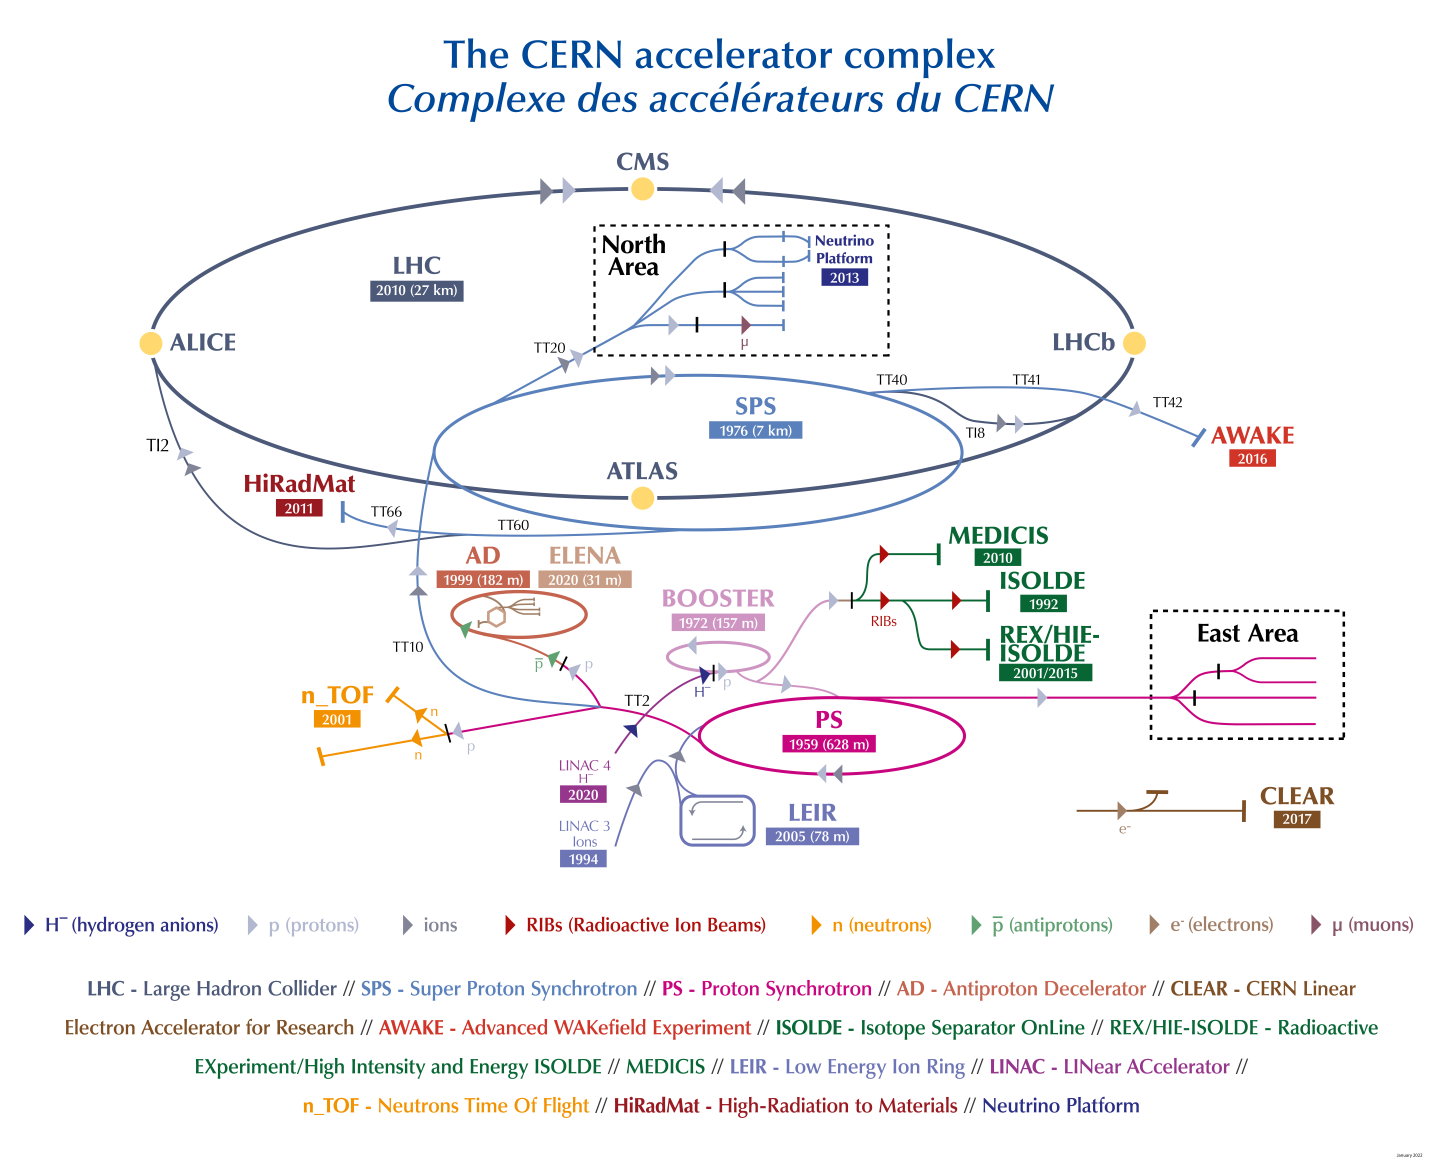
\includegraphics[width=1\textwidth]{images/cern_complex.png}
    \caption{Schematic illustration of the accelerator complex at CERN. Most accelerators are both
    used as injectors for the LHC or to provide beams to fixed target
    experiments~\cite{noauthor_cern_2022}.}
    \label{fig:introduction:cern_complex}
\end{figure}


% --------------------------------
%              LHC
% --------------------------------
\subsection{\review{The Large Hadron Collider}}

The Large Hadron Collider (LHC), is a circular particle accelerator primarily designed to collide
protons for fundamental particle physics research. It can, occasionally over the year, also collide
ions such as oxygen or lead for specifics studies. At the time of writing, in 2024, it holds several
records, such as being the largest and most powerful accelerator in the world, being near 27km long.
The LHC is composed of two beams pipes, being able to accelerate two particle beams from an
injection energy of $450$GeV to an energy of $6,800$GeV, before colliding them in four detectors:
ATLAS, CMS, Alice and LCHb.

Well publicized, the LHC is often depicted via its superconducting dipole magnets, housed in a blue
cryostat, aimed at cooling the coils. \cref{fig:3d_cut_dipole} shows a 3D cut of such magnets. The
LHC is in majority composed of those \textit{main} dipoles, as it holds $1,232$ of them, being each
about 14 meters long. Superconducting materials like Niobium-Titanium (NbTi) are utilized, as
conventional materials such as copper would melt under the current strain. There are indeed around
$12,000$ amperes supplied to generate the magnetic fields necessary for bending the trajectory of
the particles.
Those particles travel at nearly the speed of light (more precisely, $99.99999905\%$ of it),
effectively going around the tunnel about $11,200$ times per second.

\begin{figure}[!htb]
    \centering
    \includegraphics[width=0.8\textwidth]{chapters/01_Introduction/images/lhc_3D_cut.png}
    \caption{3D cut of a main LHC dipole~\cite{noauthor_cern_nodate}. Both beam pipes can be seen
    surrounded by the coils, strongly clamped by the yokes.}
    \label{fig:3d_cut_dipole}
\end{figure}


% -------------------------------
%   Straight Sections and Arcs
\subsubsection{Straight Sections and Arcs}

The LHC is not a perfect circle. It is indeed composed of four \textit{straight} sections, called
the \textit{Interaction Regions} (IPs) where detectors or specific instrumentation are placed. Connecting
those sections, the \textit{arcs} are where the majority of the magnets and their correctors are
located along with some instrument like beam position monitors.
\cref{fig:introduction:lhc_irs} shows the arcs as well as the purpose of each straight section,
housing either specific instrumentation or detectors.

\begin{figure}[!htb]
    \centering
    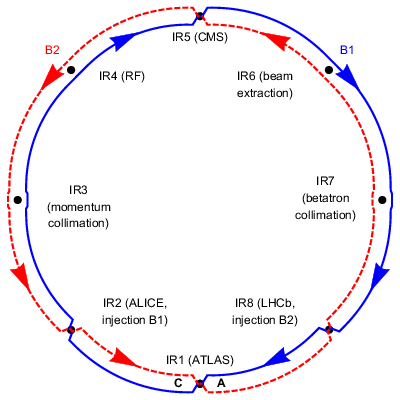
\includegraphics[width=0.5\textwidth]{./images/irs.png}
    \caption{Schematic of the LHC layout.}
    \label{fig:introduction:lhc_irs}
\end{figure}


% -------------------------------
%          Arc Cells
\subsubsection{Arc Cells}

Each arc is made up of 23 cells. Magnets are organized in a standard FoDo structure
(see \ref{section:courant_snyder}), as shows \cref{fig:introduction:lhc_arc_cell}.
\textit{Dipoles} are responsible for bending the trajectory of the particles. Their associated
correctors, the orbit correctors, mitigate any possible drift in path.
\textit{Quadrupoles} are used to control the beam size along the ring. Their effect is focusing in
one plane and defocusing in the other. Their associated correctors control the oscillations of the
beam (see tune, \ref{section:courant_snyder}) and possible field imperfections.
\textit{Sextupoles} correct chromaticity, being a misfocus from quadrupoles due to particles having
a different momentum than the reference particle.
\textit{Octupoles} are used to stabilize the beam by introducing Landau
Damping~\cite{gareyte_landau_1997}. The associated correctors correct higher order chromaticity
effects as well as amplitude dependant tune shifts.
\textit{Decapoles} correctors aim at correcting a even higher chromaticity order.

\begin{figure}[H]
    \centering
    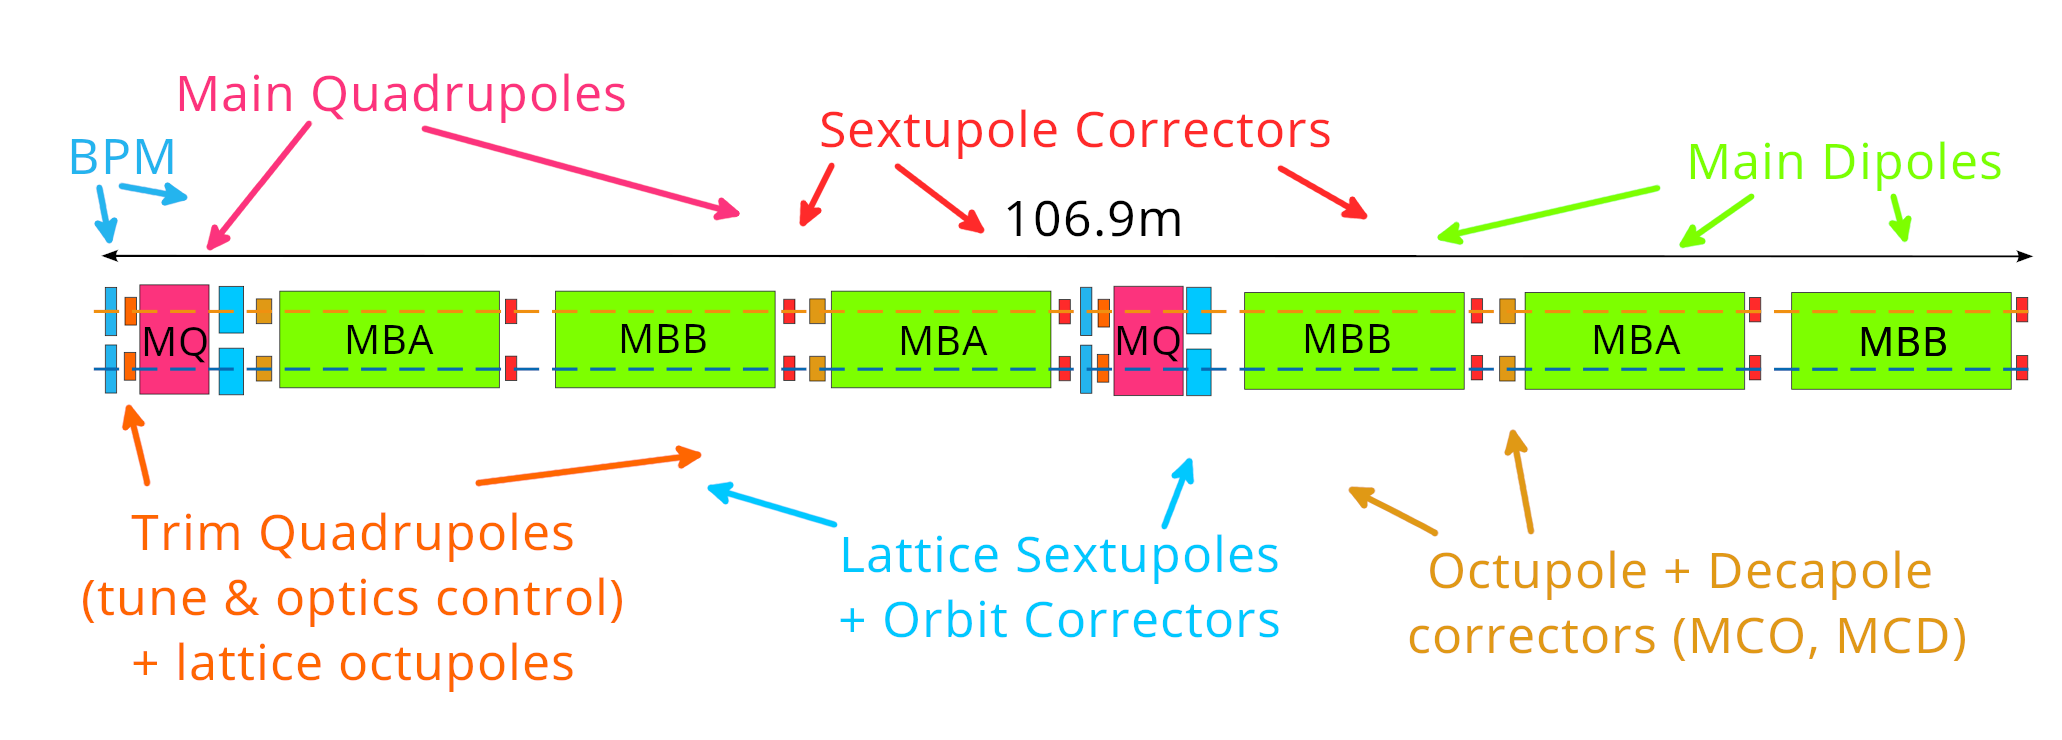
\includegraphics[width=1\textwidth]{./images/lhc_cell.png}
    \caption{Schematic of an LHC Arc cell~\cite{bruning_lhc_2004}.}
    \label{fig:introduction:lhc_arc_cell}
\end{figure}



% -------------------------------
%            Cycles
\subsubsection{\review{Cycles}}

During the operation of the LHC, the machine goes through several states. Those states of the
machine~\cite{wenniger_lhc_2019} have been defined for specific scenarios.

A common example is the operational cycle of the LHC, shown in \cref{fig:cern_complex:cycle}. The
magnets are first pre-cycled~\cite{bottura_pre-cycles_2010} without any beam circulating, to get
them back to a reproducible state. Their current is then increased to accept particles at the 
injection energy of 450GeV. In order to assess the good working condition of the machine, a probe
bunch of reduced intensity is first injected. The number of bunches and their intensity is then
ramped up to attain the desired scheme needed for collisions. This scheme varies throughout the year
depending on the demands of the experiments. The number of bunches and intensity can also be lowered
to keep the machine safe. A common scheme in 2024 is to inject about 2350 bunches with around
$10^{11}$ particles each for collisions.
Optics measurements, due to their destructive nature, typically use between one and three
\textit{pilot} bunches at a lower intensity of $10^{10}$.

The magnets current is them ramped along with the voltage injected in the RF system, to accelerate
particles to an energy of 6.8TeV. While doing so, the beam is squeezed in a first pass at the
Interaction Points. A second pass is done after the ramp is over, to reach a $\beta* = 30cm$ at the
ATLAS and CMS experiments to achieve a small beam size. Crossing-angles are then introduced to make
the beams colliding.

\begin{figure}[!htb]
    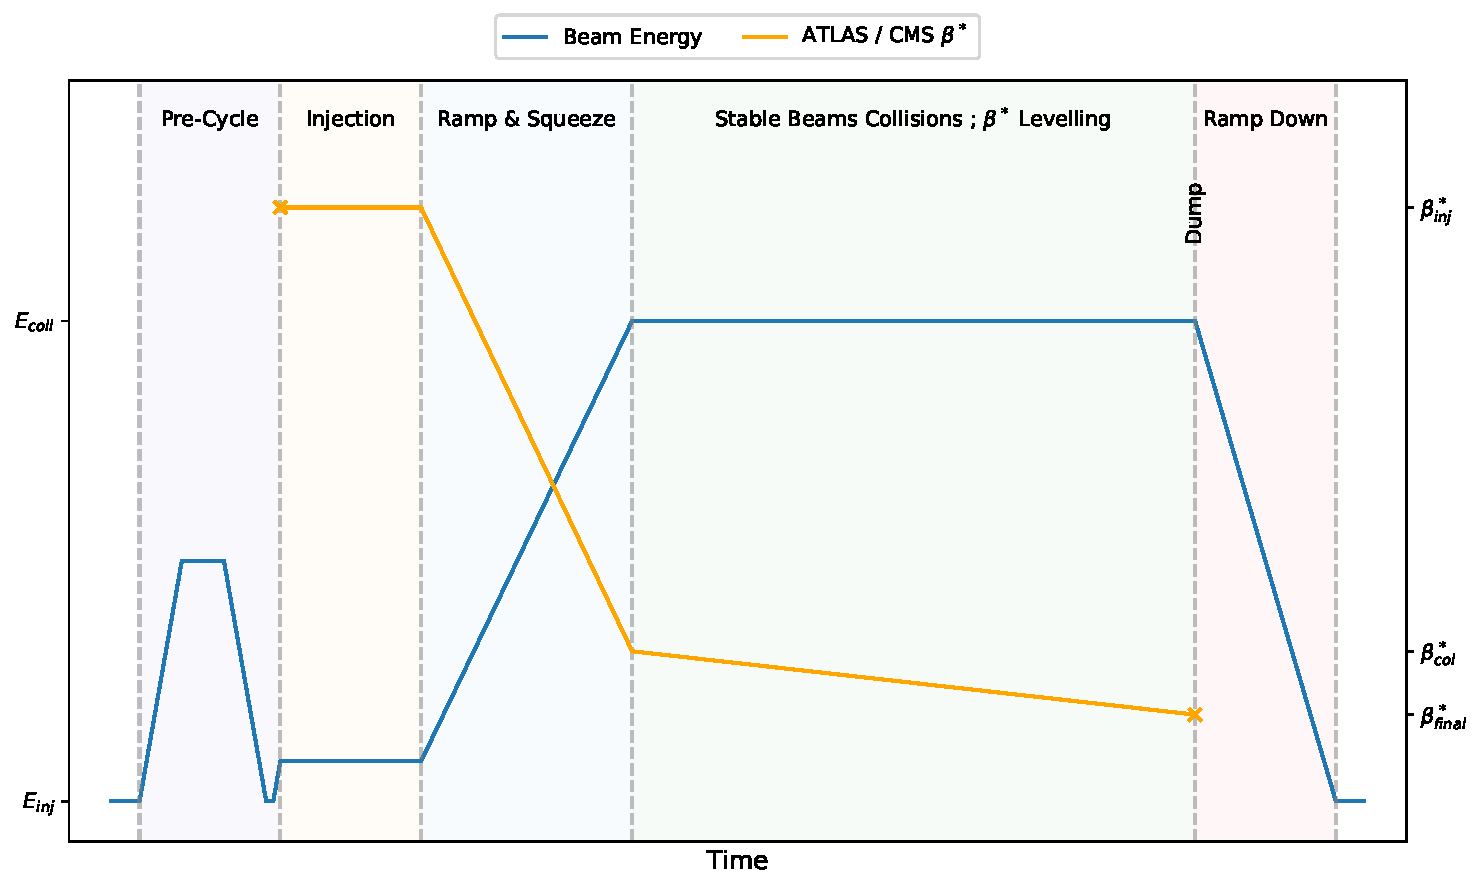
\includegraphics[width=\textwidth]{./images/lhc_cycle.pdf}
    \caption{Simplified illustration of a standard LHC cycle. Courtesy of Félix
    Soubelet~\cite{felix_soubelet_local_2023}.}
    \label{fig:cern_complex:cycle}
\end{figure}


% -------------------------------
%   Harmonics and Field Errors
\subsubsection{\review{Magnetic Fields}}

The magnetic fields of the LHC are created via the coils of the magnets. Real-life magnets never
have a single field as one would like. Instead, so called \textit{allowed harmonics} exist due to
the geometry of the coil. As such, the main dipoles of the LHC can exhibit fields similar to
sextupoles, decapoles, decatetrapoles and so on~\cite{deniau_magnetic_2009}. Manufacturing
imperfections also add fields errors outside of the scope of the allowed ones. Dipoles are indeed
found to generate octupolar field errors.

During the design of the LHC, the main dipoles have been identified to generate significant field
errors. Magnetic measurements of those various fields were thus taken and magnetic tables built
based on real-life magnets nowadays installed in the machine. Those magnetic tables, computed for
each LHC configuration by \textit{WISE}~\cite{p_hagen_wise_2006} are used by simulation softwares.
Predictions of field errors and compensating strength for the correctors is computed by the Field
Description for the LHC (\textit{FiDeL}, \cite{noauthor_fidel_2021}). FiDeL is used in the LHC
control system in operation to steer the beams.

%\begin{figure}[H]
    %\centering
    %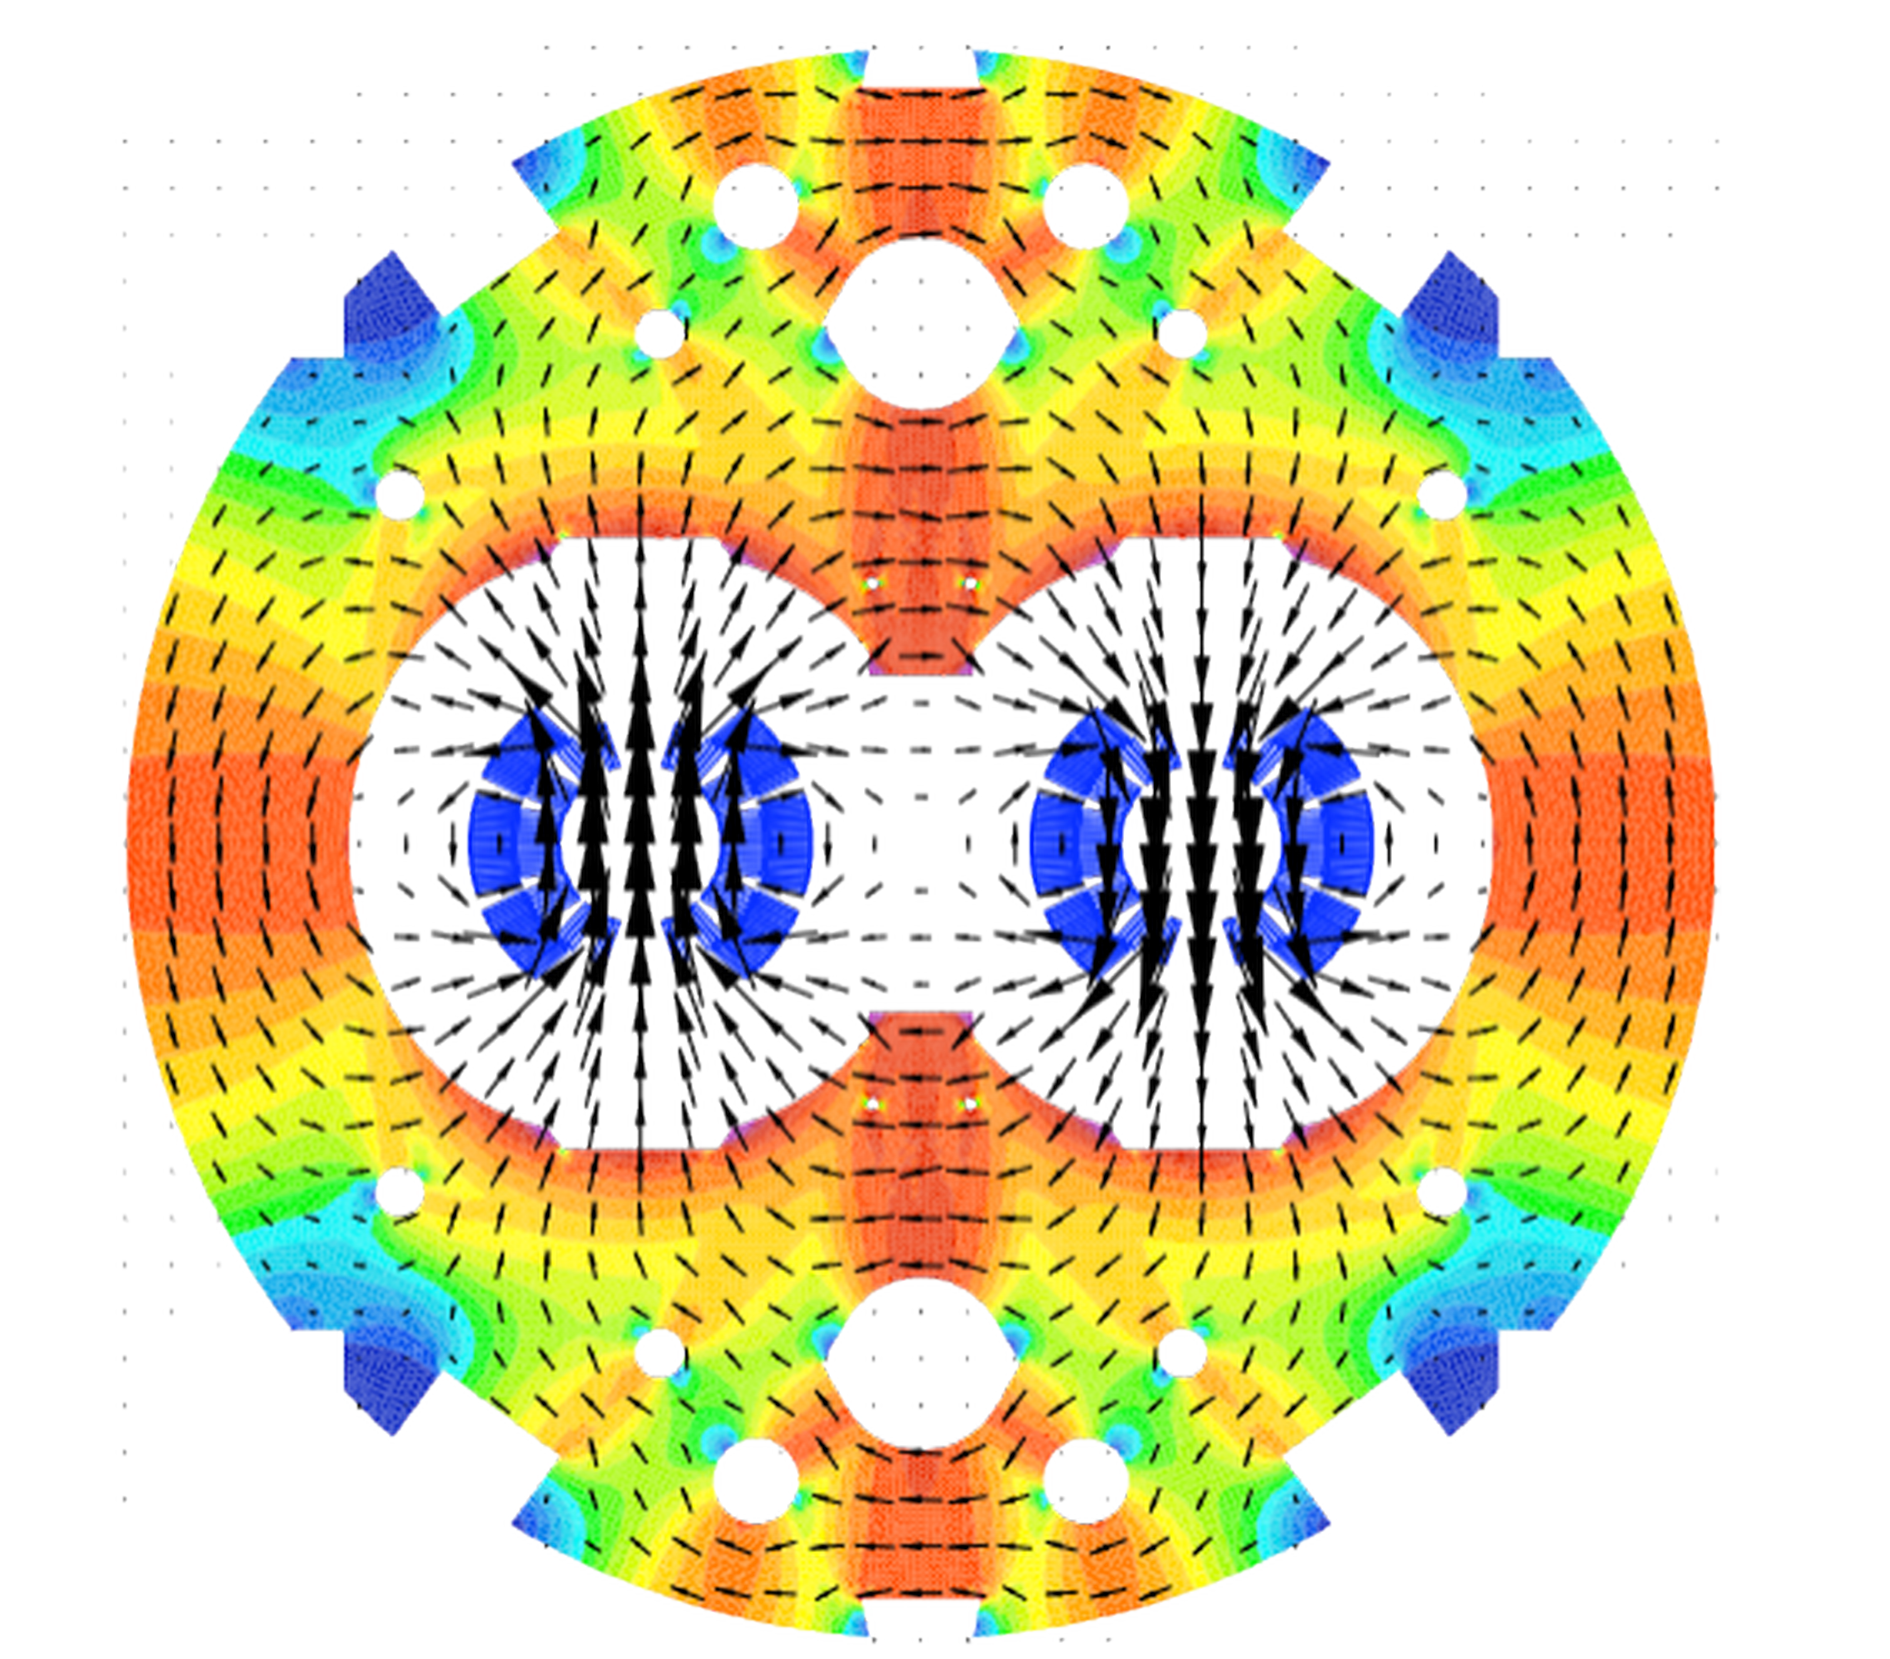
\includegraphics[width=0.5\textwidth]{./images/main_dipole_fields.png}
    %\caption{Magnetic field in a dipole magnet~\cite{deniau_magnetic_2009}.}
    %\label{fig:decapoles:magnetic_field_dipole}
%\end{figure}


% == Software
\section{\review{Tools and Softwares}}

In order to perform the measurements, analysis and simulations presented in this thesis, various
tools and softwares have been developed, used and contributed to.

Optics simulations have been done mainly in MAD-X~\cite{deniau_mad-x_nodate} and PTC.
MAD-NG~\cite{deniau_mad-ng_2020} and
Xsuite~\cite{g_iadarola_xsuite_nodate} have also been explored for specific tasks such as free RDT
simulations and GPU tracking.

Analysis of chromaticity measurements are done via a newly developed graphical
interface~\cite{m_le_garrec_non-linear_2022} written in Python. This tool makes cleaning of the raw
signal data, its analysis and results export more reliable and easier.

Overall, analysis of turn-by-turn measurements is supported by a large panel of libraries written by
the OMC team in Python and Java. Contributions have mainly been made to extended the following
packages:


\begin{itemize}
    \item \textbf{Beta-Beat GUI}~\cite{omc-team_beta-beat_2008}, Graphical interface for turn-by-turn measurements visualization and
    analysis.
    \item \textbf{OMC3}~\cite{omc-team_omc3_2021}, Main optics analysis and corrections software.
    \item \textbf{Beta-Beat.src}~\cite{omc-team_beta-beatsrc_2018}, Old analysis software, now
    replaced by OMC3.
    \item \textbf{pylhc.github.io}~\cite{omc-team_omc_2020}, Website of the OMC team with package
    documentation, examples and useful resources.
\end{itemize}

% === Concepts of Accelerator Physics
\chapter{Concepts of Accelerator Physics}
\thumbforchapter{}
\chaptertoc{}


\begin{enumerate}
    \color{red}
    \item Fields
    \begin{enumerate}
        \item Multipole Expansion
        \item Field normalization
        \item European convention
    \end{enumerate}
    \item Hamiltonian
    \item Coordinates
    \begin{enumerate}
        \item Courant Snyder, twiss parameters an phase space
        \item Linear Maps
        \item Non-Linear maps
        \item Normal Form \& RDT \& resonance diagram
    \end{enumerate}
    \item Linear optics: dispersion, coupling, momentum compaction
    \item Chromaticity

    \begin{enumerate}
        \item Combined effect of multipoles
        \item Amplitude Detuning
        \item Chromtic Amplitude Detuning
        \item Dynamic Aperture
    \end{enumerate}
    \item Luminosity
\end{enumerate}
\chapter{Optics Measurements and Corrections}
\thumbforchapter{}
\chaptertoc{}


\section{\review{Beam Instrumentation}}


% ============================================
%          Beam Position Monitors
% ============================================
\subsection{\review{Beam Position Monitors}}

Beam Position Monitors (BPMs) are one of the most utilized and essential elements of beam 
diagnostics in particle accelerators. In the LHC, most of the BPMs are dual plane, and thus composed
of four electrodes, distributed as two per plane. The BPM system consists of over than 550 BPMs pear
beam, positioned along the ring, in the arcs and the IPs. The most common type, the
\textit{curved-button}, shown in \cref{fig:beam_instrumentation_bpm_button}, is typically placed
near quadrupoles~\cite{wendt_bpm_2020}.

\begin{figure}[!htb]
    \centering
    \begin{subfigure}[b]{0.45\textwidth}
        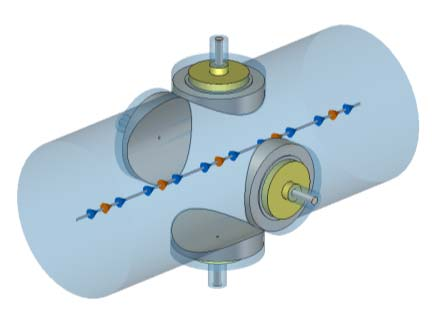
\includegraphics[width=\textwidth]{images/lhc_bpm_button.jpg}
        \caption{Button \textit{"BPM"} type BPM of the LHC~\cite{wendt_bpm_2020}.}
        \label{fig:beam_instrumentation_bpm_button}
    \end{subfigure}
    \hfill
    \begin{subfigure}[b]{0.45\textwidth}
        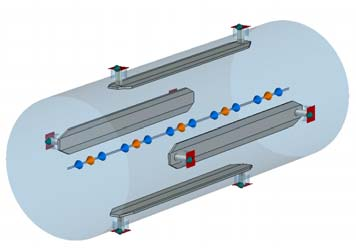
\includegraphics[width=\textwidth]{images/lhc_bpm_stripline.jpg}
        \caption{Stripline \textit{"BPMSW"} type BPM of the LHC~\cite{wendt_bpm_2020}.}
        \label{fig:beam_instrumentation_bpm_stripline}
    \end{subfigure}
\end{figure}

Other pickups such as the \textit{stripline}, shown in
\cref{fig:beam_instrumentation_bpm_stripline}, albeit more complex and expensive, offer a better
signal to noise ratio and are capable of identifying the direction of the
beam~\cite{wendt_bpm_2020}. Such features are essential for the LHC, were both beams travel through
the same aperture at the IPs.\\ 
%The BPM response is not linear with the beam position, which requires a post-processing not
%systematically implemented in accelerators beam diagnostics systems. LHC's BPMs have been simulated
%and polynomials fitted to minimize this response error~\cite{a_nosych_geometrical_2014}.


 
% ============================================
%                Collimators
% ============================================
\FloatBarrier
\subsection{\review{Collimators}}

Collimators are a crucial part of the LHC. Their purpose is to protect the machine against beam
losses and clean the outer parts of the beam~\cite{redaelli_lhc_2011}. The energy of the beams in
the LHC is high enough to not only quench the magnets, but to also damage the elements. At
injection energy, with a low intensity pilot bunch, the consequences of a loss are less severe.

%During Run 3, in 2022, a new collimator sequence was introduced, making a safe exploitation
%of the machine possible with more retracted collimators. This made measurements with higher kick
%amplitudes and larger orbit offsets, and thus momentum offsets, possible.


% ============================================
%             Beam Loss Monitors
% ============================================
\subsection{\review{Beam Loss Monitors}}

Beam Loss Monitors are detectors mounted on various elements of the accelerator, such as magnets or
collimators, to detect abnormal losses of particles. They play a crucial role in the protection of
the machine, triggering a dump when losses exceed the threshold set for their respective element. 
BLMs use ionization chambers, working on the same principle as simple Geiger counters: a tube filled
with gas, in presence of a high voltage~\cite{schmidt_machine_2014}. A picture of BLMs mounted on
the LHC is given in \cref{fig:beam_instrumentation:blm1}.

Dashboards in the control room are regularly used to monitor the losses along the ring when
performing optics measurements, as those prove to often be destructive. An example of such a
dashboard is given in \cref{fig:beam_instrumentation:blm2}.

\begin{figure}[H]
    \centering
    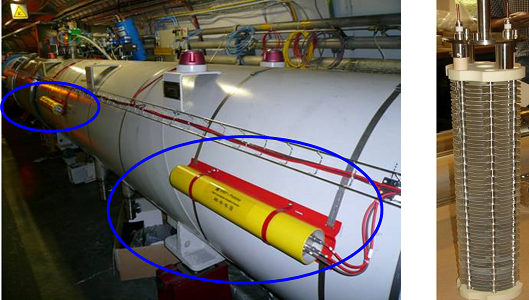
\includegraphics[width=0.6\textwidth]{images/blm.png}
    \caption{Beam Loss Monitors (BLM), in yellow, on the LHC~\cite{schmidt_machine_2014}.}
    \label{fig:beam_instrumentation:blm1}
\end{figure}

\begin{figure}[H]
    \centering
    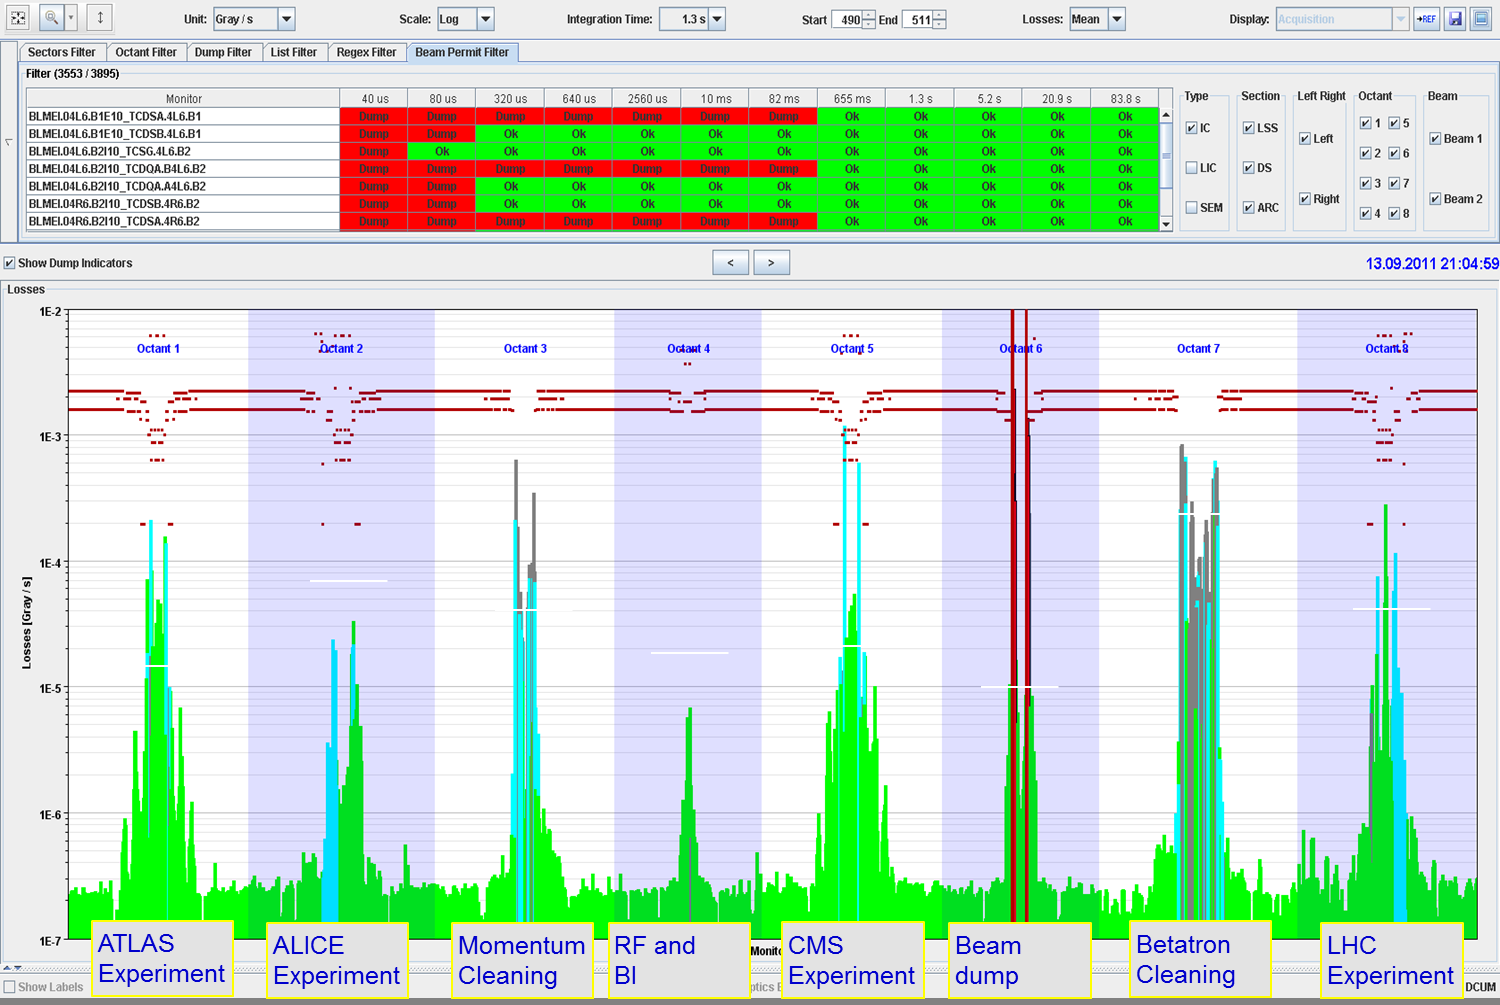
\includegraphics[width=0.6\textwidth]{images/blm2.png}
    \caption{Graphical interface used in the CERN Control Cernter (CCC) for instantaneous losses in
    the LHC~\cite{schmidt_machine_2014}. Different parts of the accelerator have varying dump
    thresholds.}
    \label{fig:beam_instrumentation:blm2}
\end{figure}


% ============================================
%                   BCT
% ============================================
\subsection{\review{Beam Current Transformer}}

The Beam Current Transformer (BCT) is a device used to measure the intensity of a particle beam by
detecting the current induced by the moving charge of the beam as it passes through the coil of the
BCT. The beam effectively acts as a primary coil and induces a current in the secondary coil of the
transformer.
The BCTs are designed to be able to measure intensities from pilots bunches of 8µA to total beams of
more than 860mA~\cite{odier_dcct_2009}. During optics measurements, beam intensity is often closely
monitored to ensure data quality, as certain observables may not be detectable at low intensities.

% ============================================
%                   BBQ
% ============================================
\subsection{\review{BBQ System}}

The Base-Band Tune (BBQ) system in the LHC is designed to measure the beam's tune via its
turn-by-turn signal. It operates by detecting and analyzing the signals of diode
peak-detectors~\cite{boccardi_first_2009,gasior_high_2005}. The system further implements processing
hardware and software, transmitting the acquired data to the control and logging systems.  The
system can operate with no explicit excitation, relying on the residual beam oscillations, or by
using tune kickers or frequency sweeps~\cite{boccardi_first_2009}.


% ============================================
%                 AC-Dipole
% ============================================
\subsection{\review{AC-Dipole}}

The AC dipole of the LHC is a crucial component for optics studies. Its primary function is to
excite the beam into large coherent oscillation, achieved by applying a sinusoidally oscillating
dipole field~\cite{miyamoto_parametrization_2008}. By ramping up and down adiabatically the
amplitude, large coherent oscillations can be produced without any decoherence or emittance growth.
\Cref{fig:ac_dipole} shows an example of a simulation made with an AC-Dipole. Exciting the beam to
large amplitudes make the study of linear optics, such as beta-beating easier, and that of non
linear optics such as resonances possible.

\begin{figure}
    \center
    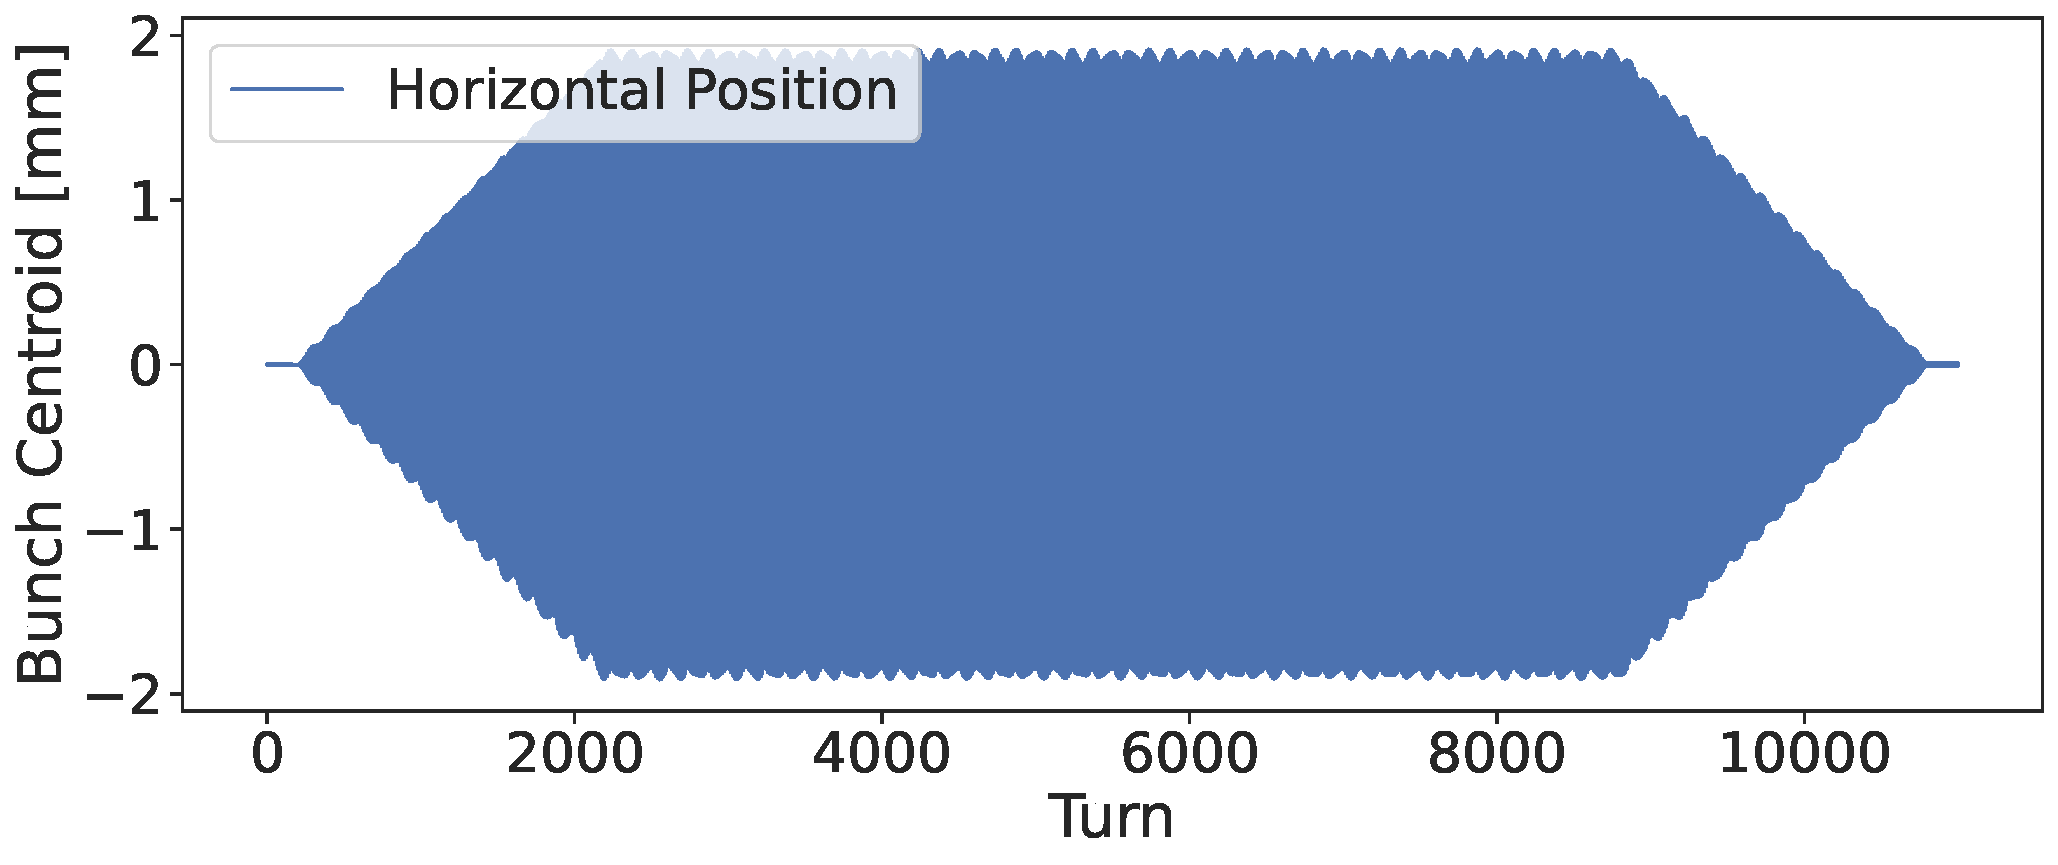
\includegraphics[width=0.85\textwidth]{./images/ac_dipole_tbt.pdf}
    \caption{Simulated turn by turn data with an AC-Dipole first ramping up then down.} 
    \label{fig:ac_dipole}
\end{figure}

The AC-Dipole is set to oscillate at a frequency $Q_d$, different from the natural tune of the
machine $Q$ and thus introduces systematic effects that needs to be compensated during the optics
analysis. The transverse position of a particle under the influence of the AC-Dipole, at turn number
$n$ and observation point $s$, is given
by~\cite{serrano_lhc_2010,tomas_normal_2002,white_direct_2013}:

\begin{equation}
z(s, n) = \frac{BL}{4\pi\rho\delta_z} \cdot \sqrt{\beta_z(s) \beta_{z,0}} \cdot \cos \left( 2 \pi Q_{d,z}n + \phi_z(s) + \phi_{z,0}\right),
\label{eq:ac_dipole}
\end{equation}

where $B$ is the amplitude of the oscillating magnetic field, $L$ the length of the AC-Dipole,
$B\rho$ the magnetic rigidity, $\delta$ the difference between $Q_d$ and $Q$, $\beta$ and $\beta_0$
the beta function at the observed point and the AC-Dipole, $\phi$ and $\phi_0$ the phase advance at
the observed point and of the AC-Dipole.
% ===============================
%        Optics Measurements
% ===============================

\subsection{Turn by Turn}





% ================================================= 
%                   Chromaticity
\subsection{Chromaticity}

% --- Procedure ---
\subsubsection{Procedure}

Chromaticity measurements are typically performed by varying the RF frequency to induce a change of momentum offset $\delta$, while measuring the tune.
The momentum offset $\delta$ being related to the RF frequency and the momentum compaction factor $\alpha_c$:

\begin{equation}
    \delta = - \frac{1}{\alpha_c} \cdot \frac{\Delta f_{RF}}{f_{RF,nominal}}
    \label{eq:dpp_rf}
\end{equation}

Frequency steps of 20Hz every 30 secondes are typically taken to compromise between number of data points, precision of the tune estimate, and duration of the measurement.
Once beam losses, registered by the Beam Loss Monitors (BLM), are deemed too high, the frequency is reverted back to its nominal value in larger steps. The same procedure is then re-applied in the negative. Figure \ref{fig:measurements:rf_scan} shows a typical RF scan performed to measure chromaticity in the LHC.

\begin{figure}[H]
    \centering
    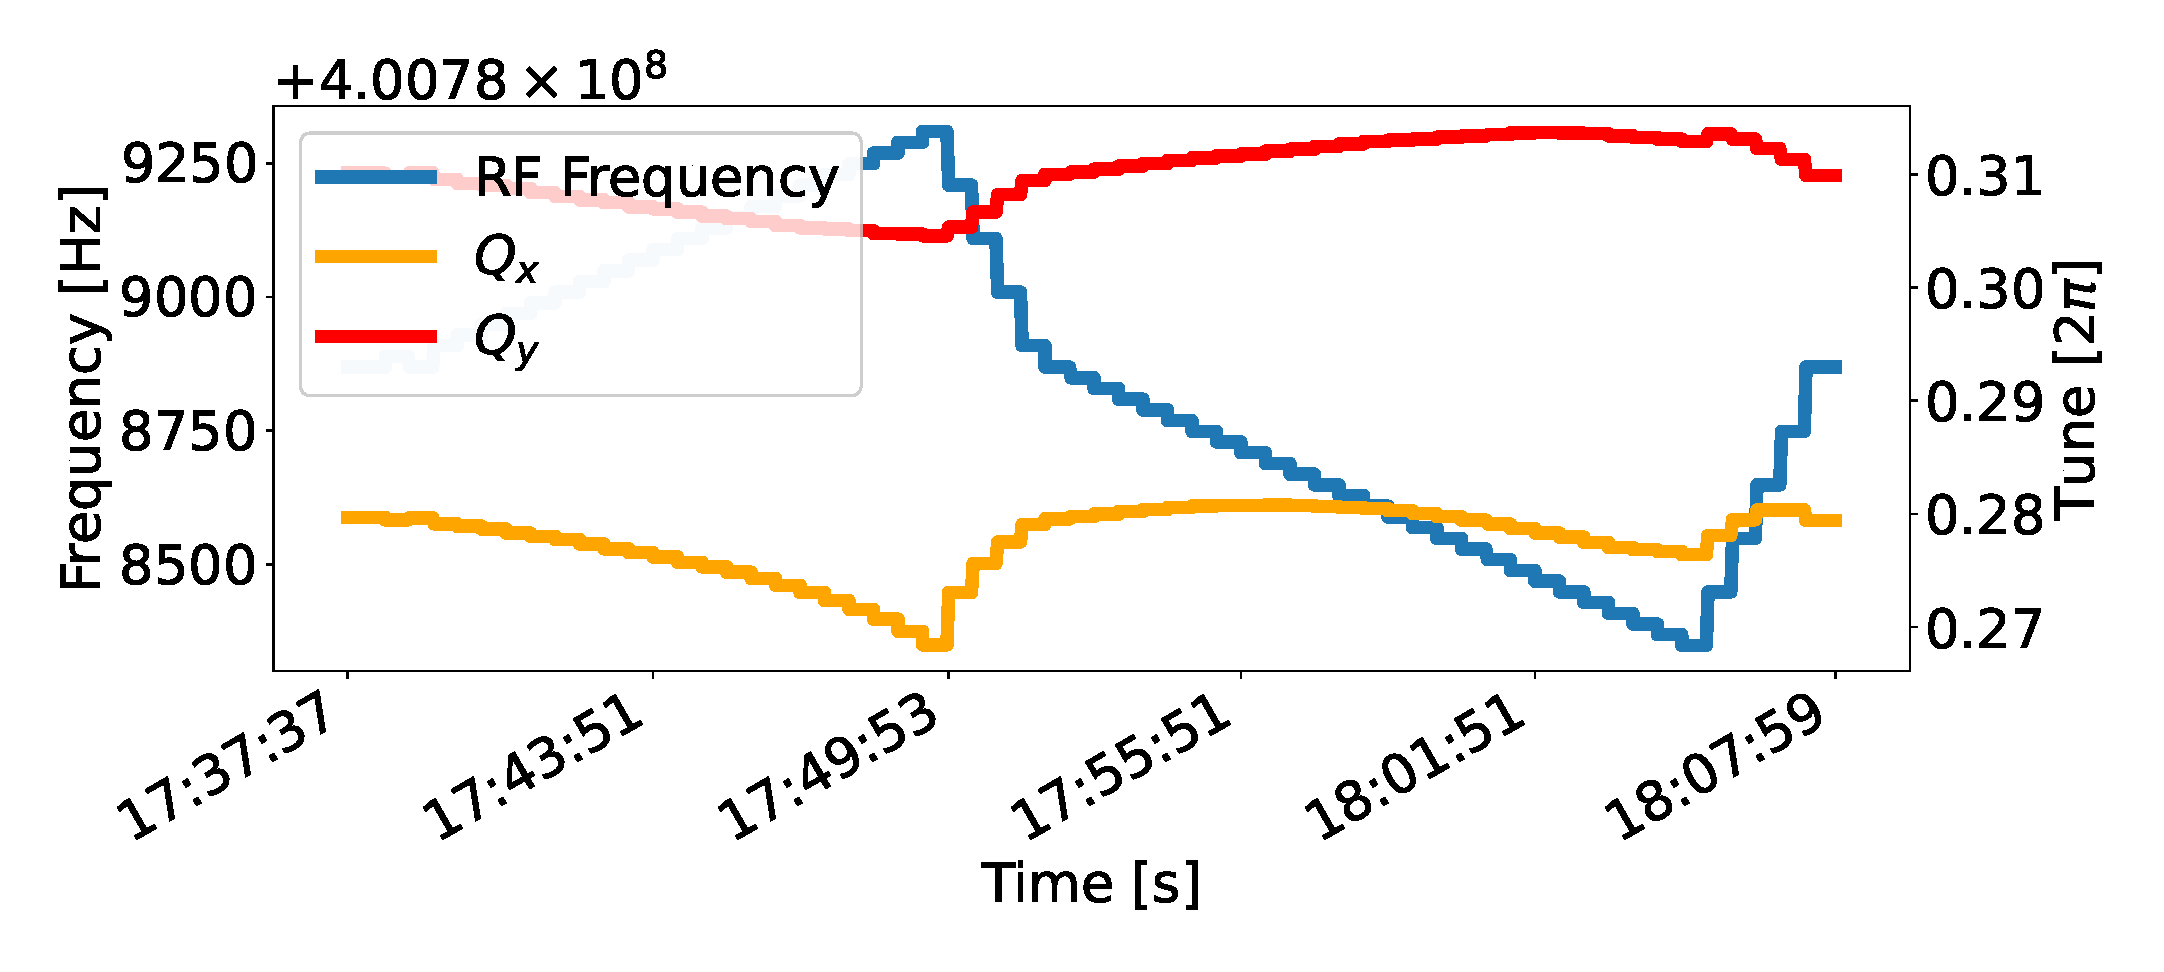
\includegraphics[width=1\textwidth]{images/rf_scan.pdf}
    \caption{Observation of the tune dependence on momentum offset, created by a shift of RF frequency}
    \label{fig:measurements:rf_scan}
\end{figure}




% --- Analysis and Fit ---
\subsubsection{Analysis}

\section{Correction Principles}


% ===============================
%        Response Matrix
% ===============================
\subsection{\review{Response Matrix}}

A response matrix is a linear equation system that describes the change of an observable for a set of individual multipole strengths. By taking the pseudo-inverse of this matrix and multiplying it to the measured observables, a set of corrector strengths if obtained that can replicate the measured value. Taking the opposite sign then gives a correction.
This technique is routinely used to correct, amongst others, \beta-beating as well as Resonance Driving Terms. In situations where measurements are taken at each BPM for a particular observable, the corresponding response matrix ends up containing over 500 values per corrector, for a single beam.

Individual MAD-X simulations are run with a single multipole powered at a time. The resulting parameter values (e.g. \beta-beating) are then compared to those obtained from a simulation without any powering, allowing to determine the specific impact of each multipole.

A response matrix is thus created following eq.\ref{eq:resp_matrix}, for a matrix of observables $O$, a reference matrix of observables without any corrector $O_R$ and a fixed multipole strength $k$. Given measured data $M$, the set of correctors needed to compensate the values can be obtained by taking the pseudo-inverse of the matrix in eq.\ref{eq:resp_matrix_inverted}.

\begin{equation}
  R = \left(O - O_R \right) \cdot \frac{1}{k}
  \label{eq:resp_matrix}
\end{equation}

\begin{equation}
  \begin{bmatrix}
    k_1 \\
    \vdots \\
    k_n \\
  \end{bmatrix}
  = -(R^{+} \cdot M)
  \label{eq:resp_matrix_inverted}
\end{equation}
 
Response matrices are very versatile and can combine several observables to be corrected by the same multipoles. One example, detailed later in this thesis, is the third order chromaticity and the resonance driving term $f_{1004}$, both contributed to by decapoles.

\subsubsection{Example}

In this example, simulations are run with MAD-X PTC to correct the third chromaticity in the LHC.
$Q'''$ is taken from \verb|ptc_normal| for each beam and axis, with \verb|MCDs|, decapole correctors, powered with a fixed strength one at a time. A scaling factor is applied to get the change of chromaticity for one unit of $K_5$.
8 correctors are used, which strengths are denoted $k_1$ through $k_8$.
Transposes are only used to make the equations easier to display.\\
The values in Tab.\ref{table:resp_matrix_example} are corrected via 
Eq.~\eqref{eq:resp_matrix_inverse_example} after having built the response matrix in Eq.~\eqref{eq:resp_matrix_example}.

\begin{table}[H]
  \center
  \begin{tabular}{c c c}
      Observable & Value \\
      \hline
      $Q'''_x$ & -666111 \\
      $Q'''_y$ &  121557 \\
  \end{tabular}
  \caption{Example chromaticity values to correct via a response matrix}
  \label{table:resp_matrix_example}
\end{table}

% ====
\vspace{0.4cm}
\begin{equation}
  R
  %
  =
  %
  \left(
    %{\text{Individual} \atop \text{simulations}}
    {\genfrac{}{}{0pt}{0}{\text{Individual}}{\text{simulations}}}
    \left\{
      \begin{bNiceMatrix}
       -155899  &  122004 \\  
       -254584  &  138368 \\
       -122715  &  106709 \\
       -218597  &  110686 \\
       -134140  &  106463 \\
       -245791  &  118951 \\
       -147035  &  116544 \\
       -219537  &  112317 \\
        \CodeAfter
        \OverBrace{1-1}{1-1}{Q'''_x}[yshift=2mm]
        \OverBrace{1-2}{1-2}{Q'''_y}[yshift=2mm]
      \end{bNiceMatrix}^T
    \right.
    -
    \left.
    \begin{bNiceMatrix}
       5135 \\
       8470 \\
      \CodeAfter
      \OverBrace{1-1}{1-1}{\scriptstyle \text{Reference}}[yshift=2mm]
    \end{bNiceMatrix}
    \right\}
    {\genfrac{}{}{0pt}{0}{Q'''_x}{Q'''_y}}
  \right)
  %
  \cdot
  %
  \underbrace{\frac{1}{-1000}}_{\text{Corrector strength}}
  \label{eq:resp_matrix_example}
\end{equation}
\vspace{0.5cm}


% Inverting the response matrix
\begin{equation}
    \begin{matrix}
      k_1 \\
      k_2 \\
      k_3 \\
      k_4 \\
      k_5 \\
      k_6 \\
      k_7 \\
      k_8 \\
    \end{matrix}
  \left\{
  \begin{pmatrix}
     -1235 \\
      1032   \\  
     -1394  \\ 
      1449   \\ 
     -1043  \\ 
      1864   \\ 
     -1187  \\ 
      1369   \\ 
  \end{pmatrix}
  \right.
  %
  =
  %
  -R^{+} 
  %
  \cdot
  %
  \left.
  \begin{pNiceMatrix}
      -666111 \\
      121557 \\
  \end{pNiceMatrix}
  \right\}
  %{\text{Measured} \atop \text{values}}
  {\genfrac{}{}{0pt}{0}{\text{Measured}}{\text{values}}}
  \label{eq:resp_matrix_inverse_example}
\end{equation}





% ===============================
%    Chromaticity Global Trim
% ===============================
\subsection{\review{Global Trims for Chromaticity}}

% ~~~~~~~~~~~~~~~~~~~~~~~~~~~~~
% The script for the linearity can be found in
% /afs/cern.ch/work/m/mlegarr2/public/jupyter/chromaticity/simulations/linearity_dq3_mcd

As per the placement of the MCO and MCD spool piece correctors in the LHC 
layout~\cite{maclean_commissioning_2016-1}, $\beta$-functions at their location are slightly
different from arc to arc. This slight imbalance leads theoretically to the possibility of
correcting the horizontal and vertical axes of the second and third order chromaticity
independently, via a response matrix approach. In practice, the required strength to do so would
exceed those of the design of the correctors.

Another way to correct the chromaticity is via a global uniform trim, where every available
corrector is powered to the same strength.  Simulations are run with \verb|ptc_normal| via MADX-PTC
to obtain the response in chromaticity for a given strength. Chromaticity being linear with
multipole strength, an affine function can be determined for each axis. Figure
\ref{fig:corrections-dq3_versus_k5} shows a simulation with several MCD strengths, highlighting this
linear relation between $Q'''$ and $K_5$, while
Equation~\eqref{eq:corrections:chromaticity_affine_function_ptc} shows an example of such functions computed
at injection energy for the 2022 optics.

\begin{figure}[H]
  \centering
  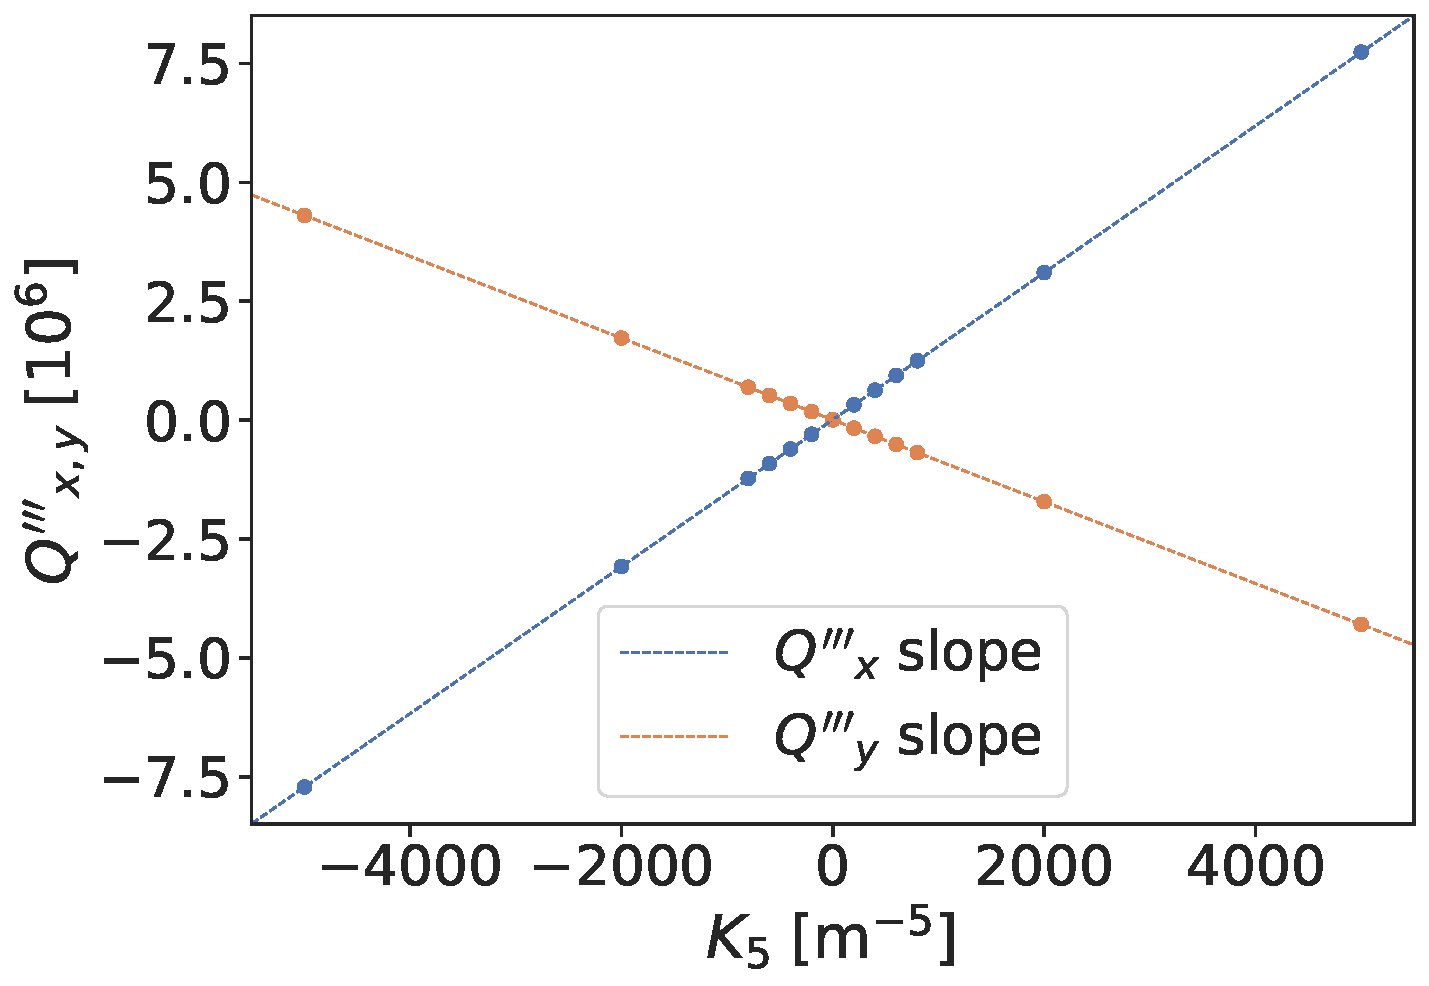
\includegraphics[width=0.6\textwidth]{images/dq3_k5.pdf}
  \caption{Linear relation between the third order chromaticity and decapole corrector strengths,
           simulated with MADX-PTC.}
  \label{fig:corrections-dq3_versus_k5}
\end{figure}

\begin{equation}
  \begin{aligned}
    &Q'''_x = 1533 \cdot \Delta K_5 + 6680 \\
    &Q'''_y = -860 \cdot \Delta K_5 + 5647
  \end{aligned}
  \label{eq:corrections:chromaticity_affine_function_ptc}
\end{equation}

Only the linear part is relevant, as the offset is generated by other multipoles and field errors.
It is thus constant for a configuration where only the relevant spool pieces are used.

Corrections involve minimizing both axes, typically where $Q'''_x$ meets $Q'''_y$:

\begin{equation}
  \Delta K_5 = -\frac{(Q'''_x - Q'''_y)}{\text{slope}_{Q'''_x} - \text{slope}_{Q'''_y}}
  \label{eq:corrections:chromaticity_global_correction}
\end{equation}
\chapter{Decapole Measurements, Corrections and Modelling in the LHC}
\thumbforchapter{}
\chaptertoc{}
\newpage

% === Motivation
\section{Motivation}

The decapole fields in the LHC have been studied since Run 1 via chromaticity 
measurements~\cite{maclean_non-linear_2011,maclean_commissioning_2016,maclean_measurement_2014}. 
The third order of the non-linear chromaticity, $Q'''$, generated for the most part by decapoles,
has shown a consistent discrepancy at injection energy between its expected value in simulation and
that observed in beam-based mesurements.
Figure \ref{fig:decapoles:bare_chroma_vs_simulations} highlights this discrepancy.

\begin{figure}[H]
    \centering
    \captionsetup{justification=centering,margin=2cm}
    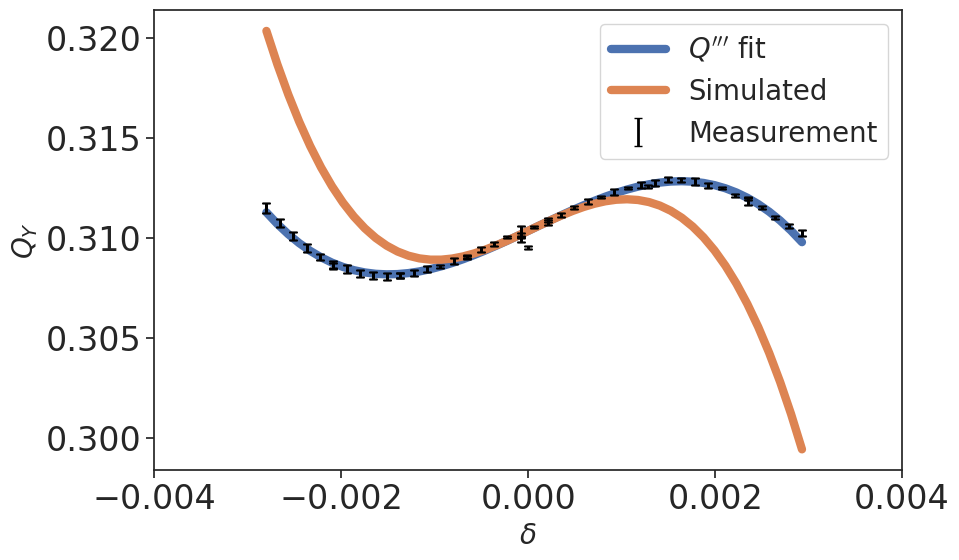
\includegraphics[width=0.7\textwidth]{images/bare_chroma_simulated.png}
    \caption{Measured and simulated chromaticity at injection energy without octupolar and
             decapolar corrections.}
    \label{fig:decapoles:bare_chroma_vs_simulations}
\end{figure}

This discrepancy poses a significant problem, as the operational corrections are derived from
simulations. It is thus observed that $Q'''$ is over-corrected by an almost factor 2, resulting in
an effectively un-corrected third order chromaticity.
Chromaticity measurements have thus been repeated during LHC's Run 3 and complemented by beam-based
corrections.

While non-linear chromaticity provides an easy measurement of decapolar fields, it does not permit
alone to understand where the discrepancy originates from. 
New measurements were therefore undertaken to better understand the decapolar fields via observables
never studied before:
\begin{itemize}
    \tightlist
    \item Bare Chromaticity, chromaticity with octupolar and decapolar correctors turned off.
    \item Chromatic Amplitude Detuning, tune shift dependant on both the action and the momentum 
    offset.
    \item Resonance Driving Term $f_{1004}$, contributing to a resonance close the working point.
\end{itemize}



% ===================
%    Chromaticity
% ===================


% Correction
%\paragraph{Correction}
%
%$Q'''$ is linear with the decapole strength. As such, it can be easily corrected via global trims
%presented in~\cref{subsection:correction_chromaticity}.
%A change of decapole strength $K_5 = 1000$ would for example have the following impact with the
%injection optics used in 2022:
%
%\begin{equation}
%    \begin{aligned}
%        \Delta Q'''_x =  1.5 \times 10^6 \quad;\quad
%        \Delta Q'''_y = -0.9 \times 10^6.
%    \end{aligned}
%\end{equation}






%\subsection{\todo{blabla}}
%
%Measurements were taken during 2022 Commissioning for 
%\begin{itemize}
%    \item Beam Test
%    \item Commissioning
%    \begin{itemize}
%        \item FiDeL
%        \item Q''' corr
%        \item Q'' corr
%    \end{itemize}
%    \item 60° optics
%\end{itemize}
%
%Also during MD6864, 2022-10-19, for the bare machine \\
%Also 2022-11-06, measurement at 30cm, flat top.
%

% ===============================
%        Corrector Response
% ===============================
\section{\review{Response of correctors}}

% ===============================
%         Introduction
\paragraph{Expression}

The full third term of the chromaticity function is highlighted in
\cref{eq:decapoles:chromaticity_highlight}. Details on chromaticity are given
in \cref{subsection:concepts:chromaticity}.

\begin{equation} 
    Q (\delta) = Q_0 + Q' \delta + \frac{1}{2!} Q'' \delta^2 
                     + \colorbox{yellow!50}{$\displaystyle  \frac{1}{3!}  Q''' \delta^3$}
                     + \mathcal{O}(\delta^4).
    \label{eq:decapoles:chromaticity_highlight}
\end{equation}

This third order, mainly contributed to by decapoles, is related to the $\beta$-function, the
dispersion and the strength of the multipole:

\begin{equation}
    \begin{aligned}
        \Delta Q_x''' &=  &\frac{1}{4\pi} K_{5} L \beta_x D_x^{3}\\
        \Delta Q_y''' &= -&\frac{1}{4\pi} K_{5} L \beta_x D_x^{3}.
    \end{aligned}
\end{equation}


% 2022-04-24
\paragraph{Measurements and Corrections}

In order to assess the accuracy of corrections, measurements have to be done to gauge the response
of the decapolar correctors, \textit{MCDs}.
During Run~3's commissioning, measurements and corrections of $Q''$ and $Q'''$ have been made
routine. Those corrections give the opportunity to study the response of the correctors.
\cref{figure:decapoles:chromaticity:dq3_comparison} shows the chromaticity function measured during
Run~3's commissioning in 2022 with the nominal corrections via FiDeL and beam-based corrections
computed analytically based on top of FiDeL.

\begin{figure}[H]
    \centering
    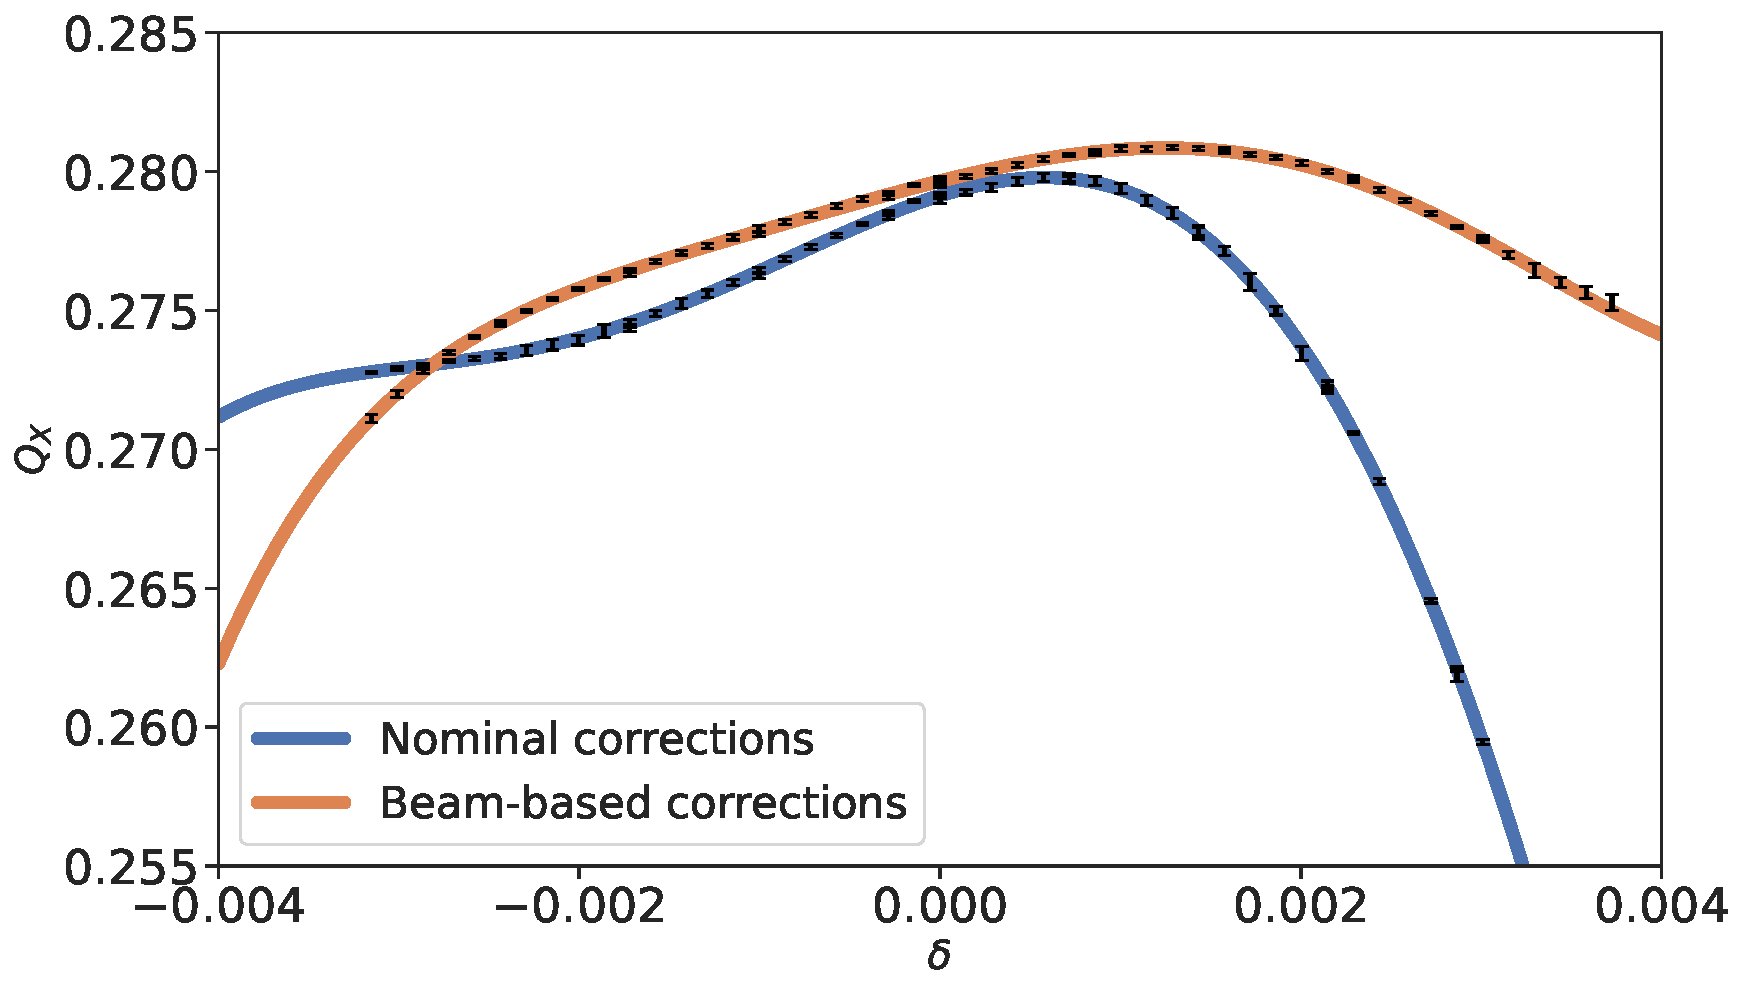
\includegraphics[width=0.8\columnwidth]{images/nominal_vs_beam_based_corrections.pdf}
    \caption{Chromaticity of the horizontal plane of Beam 1 during Run 3's commissioning, with
    nominal corrections based on the magnetic model and beam-based corrections aimed at correcting
     $Q''$ and $Q'''$.}
    \label{figure:decapoles:chromaticity:dq3_comparison}
\end{figure}

The nominal and corrected $Q'''$ values are shown in
\cref{table:decapoles:chromaticity:dq3_before_after_beam_based}. The shift in $Q'''$ is shown for
each beam and axis, showing a good agreement between the measurement and the simulation.
The slight imbalance can be attributed to higher order effects of the octupole correctors, whose
correction was implemented after that of $Q'''$.

\begin{table}[H]
    \centering
    \begin{tabular}{|l||r|r|r|c|}
    \hline
              &  \multicolumn{2}{c|}{$Q''' [10^6]$}  &  \multicolumn{2}{c|}{$\Delta Q''' [10^6]$}\\ \hline\hline
        B1    &   \multicolumn{1}{c|}{Nominal}     &   \multicolumn{1}{c|}{Beam-based}   & Measured & Simulated \\
        X     &  -3.36 ± 0.04 &  -1.02 ± 0.03  &  2.3 ± 0.1 &   2.5 \\
        Y     &   1.62 ± 0.05 &   0.12 ± 0.02  & -1.5 ± 0.1 &  -1.4 \\ \hline
        %B2    &   \multicolumn{1}{c|}{Nominal}     &   \multicolumn{1}{c|}{Beam-based}   &&\\
        B2    &               &&& \\
        X     &  -2.72 ± 0.08 &  -0.64 ± 0.03  &  2.1 ± 0.1 &  2.5\\
        Y     &   1.54 ± 0.06 &   0.14 ± 0.03  & -1.4 ± 0.1 & -1.4\\ \hline
    \end{tabular}
    \caption{Third order chromaticity obtained during Run~3 commissioning, with nominal and
    beam-based corrections aimed at correcting $Q''$ and $Q'''$.
    The change in $Q'''$, measured and expected via simulations, is also shown.} 
    \label{table:decapoles:chromaticity:dq3_before_after_beam_based}
\end{table}


This agreement between the simulations and the measurements indicates that our decapole correctors
function as intended. No noticeable cross-talk between magnets or hysteresis have been identified.



% ===============================
%        Bare Chromaticity
% ===============================
\section{\review{Bare Chromaticity}}


% 2022-10-19

Previous studies~\cite{maclean_measurement_2014} have demonstrated that octupole and decapole
correctors were contributing to an observed octupolar discrepancy in the machine via hysteresis and
feed-down. To evaluate the possible effect of decapole correctors on the third order chromaticity
$Q'''$, a measurement was taken with these elements turned off.

\begin{figure}[H]
    \begin{subfigure}{0.49\textwidth}
        \centering
        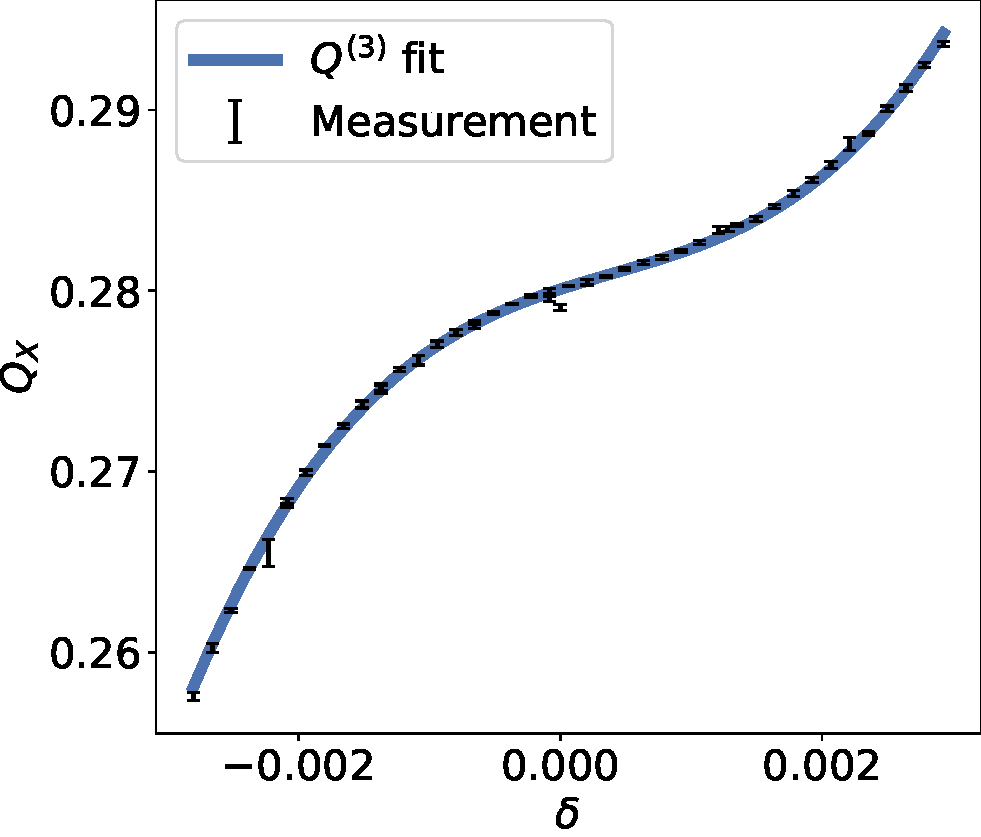
\includegraphics[width=\textwidth]{./images/bare_chromaticity/Beam1_Qx.pdf}
        \caption{$Q_x$ Beam 1}
        \label{}
    \end{subfigure}
    \hfill
    \begin{subfigure}{0.49\textwidth}
        \centering
        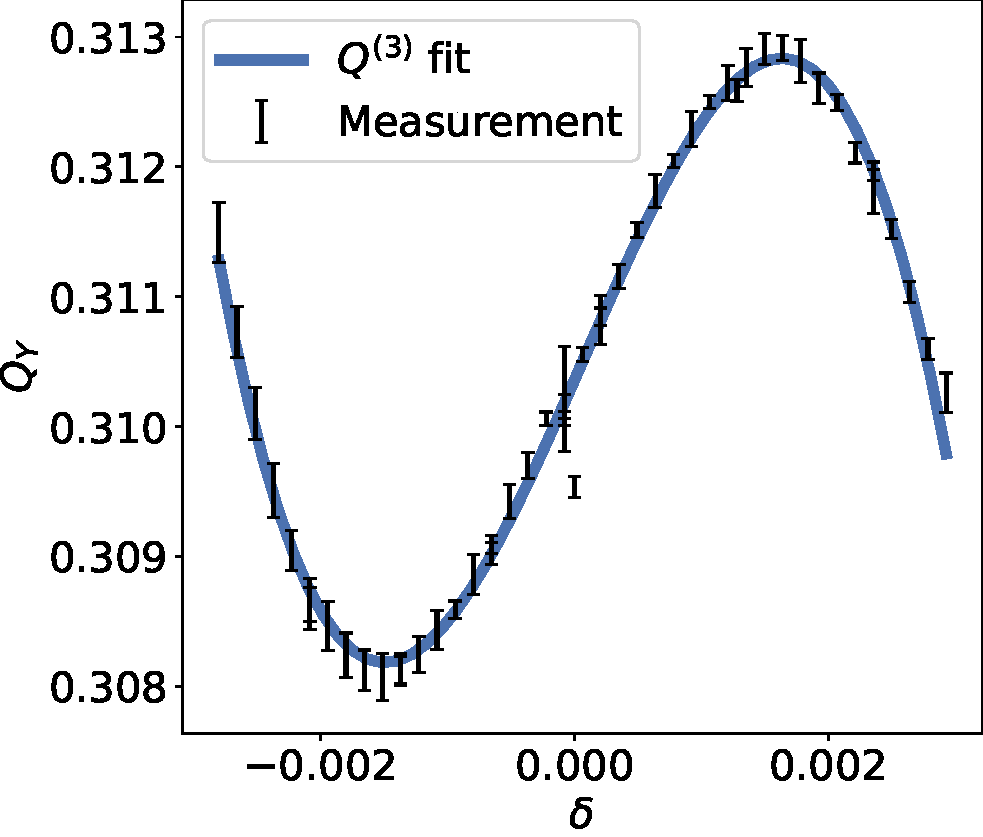
\includegraphics[width=\textwidth]{./images/bare_chromaticity/Beam1_Qy.pdf}
        \caption{$Q_y$ Beam 1}
        \label{}
    \end{subfigure}
    %
    \\
    %
    \begin{subfigure}{0.49\textwidth}
        \centering
        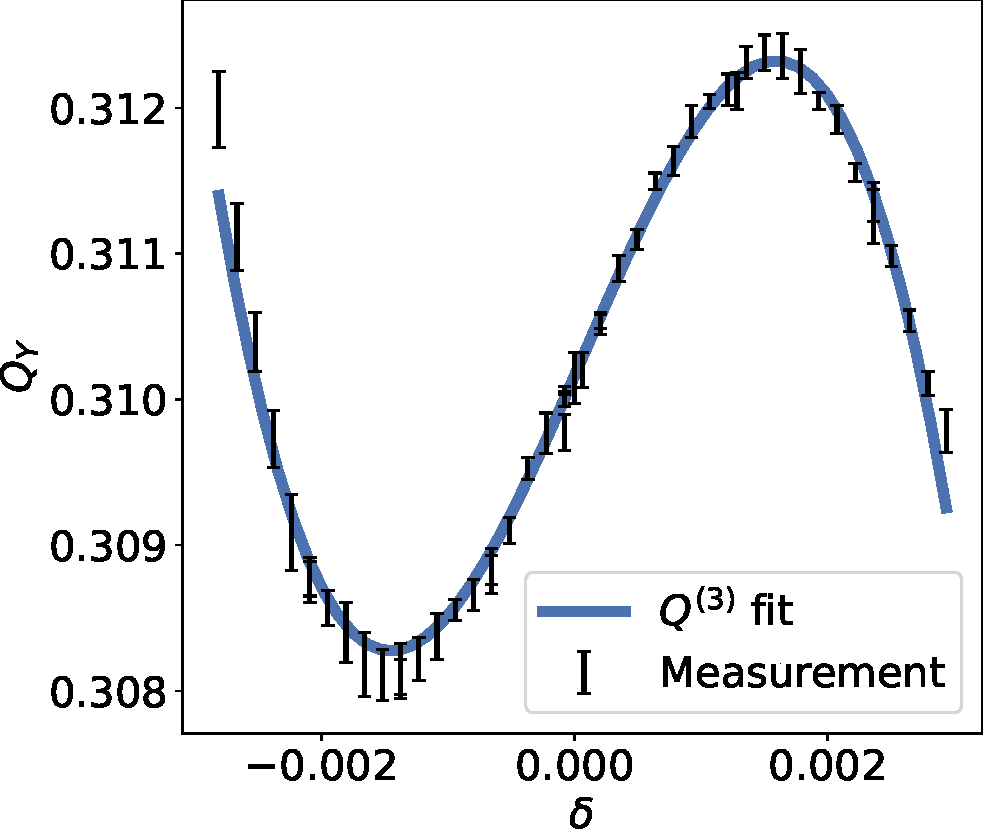
\includegraphics[width=\textwidth]{./images/bare_chromaticity/Beam2_Qy.pdf}
        \caption{$Q_x$ Beam 2}
        \label{}
    \end{subfigure}
    \hfill
    \begin{subfigure}{0.49\textwidth}
        \centering
        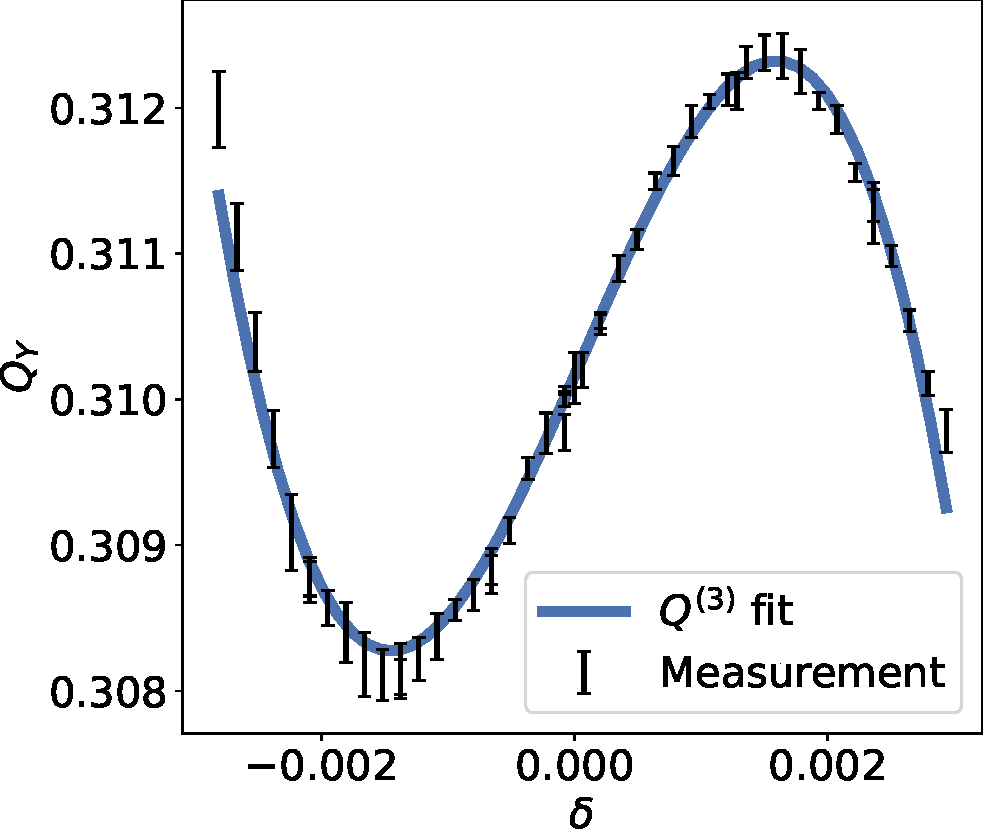
\includegraphics[width=\textwidth]{./images/bare_chromaticity/Beam2_Qy.pdf}
        \caption{$Q_y$ Beam 2}
        \label{}
    \end{subfigure}
    \caption{Fit of the chromaticity function for the chromaticity measurement performed with 
    octupole and decapole correctors powered off. The fit includes all orders up to third.}
    \label{fig:decapoles:bare_chromaticity}
\end{figure}

Simulations have been run with MAD-X and PTC including fields errors from $b_3$ to $b_8$. The
expected $Q'''$ values are presented in~\cref{table:decapoles:bare_chromaticity:virgin_dq3} and
compared to the measured ones along with the ratio between the two.

\begin{table}[tbh]
    \centering
    \begin{tabular}{|l||r|r|r|}
    \hline
        Plane     &  Meas. $Q''' [10^6]$        &  Sim. $Q''' [10^{6}]$          &   Ratio     \\\hline\hline
        Beam 1    &                             &                                &             \\
                X &            2.95 ± 0.04      &         6.94 ± 0.02            &  0.43 ± 0.01  \\
                Y &           -1.82 ± 0.04      &        -4.29 ± 0.01            &  0.42 ± 0.01  \\ \hline
        Beam 2    &                             &                                &             \\
                X &            3.06 ± 0.07      &        7.03 ± 0.02             &  0.44 ± 0.01 \\
                Y &           -1.72 ± 0.02      &       -4.27 ± 0.01             &  0.42 ± 0.01  \\ \hline
    \end{tabular}
    \caption{Measured and simulated third order chromaticity with octupole and decapole correctors
    turned off. The simulations include field errors from sextupoles to decahexapole ($b_3$ to
    $b_8$).}
    \label{table:decapoles:bare_chromaticity:virgin_dq3}
\end{table}

A consistent ratio is observed for every plane and axis between the measurement and the model. This
result, supplemented by the correct response of the correctors, indicates that the decapolar
correctors do no generate unwanted fields. Those correctors can thus be discarded as the potential
source of discrepancy.


% === Chromatic Amplitude Det
\section{Chromatic Amplitude Detuning}

% === RDTs
\section{Resonance Driving Terms}

Measurements 

\begin{itemize}
    \item 2022 Q'' and Q''' corrs 2022-04-24
    \item 2022-10-19 Virgin machine
    \item 2023-easter (FiDeL)
    \item 2023-06-14 MD9549 (FiDeL and Q'''/ RDT corr)
\end{itemize}

Bring up effect of KCO on RDT f1004

\subsection{Decapolar Contribution}

\subsection{Lower Order Contributions}

\section{Impact of Decapolar Fields}

\section{Integrating Decay}
\chapter{\todo{Higher Order Fields}}
\thumbforchapter{}
%\chaptertoc{}
\newpage


%====================
% 	Introduction
%====================
\section{\review{Introduction}}

Beam-based high order field measurements have been carried out in the LHC since its first
Run~\cite{maclean_non-linear_2011, maclean_commissioning_2016-1}, via
chromaticity studies. Those measurements, made by varying the RF frequency while observing the
resulting tune change, have been performed with a momentum offset of up to $\delta = \pm 2.2 \times
10^{-3}$, which led to the observation of the third order term of the non-linear chromaticity.

During the commissioning of Run~3 in 2022, a new collimator sequence has been introduced, allowing wider
momentum offset measurements, within $\delta \in [-3.2\times 10^{-3},3.7 \times 10^{-3}]$. This
improved setup led to the observation of the fourth and fifth order terms at injection energy.
Those terms, denoted $Q^{(4)}$ and $Q^{(5)}$ respectively in
\cref{eq:very_high_orders:chromaticity_high_orders}, are produced to first order by dodecapoles and
decatetrapoles. Dodecapoles being powered off at injection and decatetrapoles being absent from the
lattice, those fields originate from the field errors of the various magnets installed in the LHC.

\begin{equation}
  \begin{aligned}
    Q(\delta) = Q_0 + Q'\delta &+ \frac{1}{2!}Q''\delta^2 + \frac{1}{3!}Q'''\delta^3
                                + \frac{1}{4!}Q^{(4)}\delta^4  + \frac{1}{5!}Q^{(5)}\delta^5
                                + \mathcal{O}(\delta^6).
  \end{aligned}
  \label{eq:very_high_orders:chromaticity_high_orders}
\end{equation}


In addition to completing the measurements of high-order fields through chromaticity scans,
turn-by-turn measurements were also conducted. High amplitude kicks indeed made it possible to
observe dodecapolar RDTs in the LHC for the first time. Such fields were never before observed
directly, but rather only via feed-down to amplitude detuning~\cite{dilly_corrections_2022}.



%=============================
%        Chromaticity
%=============================
\section{\review{Chromaticity}}
\label{section:very_hgih_orders:chromaticity}

As described in \cref{subsection:optics_corrections_chromaticity}, the momentum offset $\delta$ is
related to the RF frequency and the momentum compaction factor. This relation is given as a
simplified form in \cref{eq:very_high_orders:simplified_eq_momentum_compaction}, neglecting the
Lorentz factor $\gamma$. 
The model $\alpha_c$ for the LHC injection optics is $3.48 \times 10^{-4}$ for beam 1 and $3.47
\times 10^{-4}$ for beam 2. Via this relation, a change of 140Hz of the RF frequency corresponds to
a momentum offset of about $-0.001$.

\begin{equation}
    \delta = -\frac{1}{\alpha_c} \cdot \frac{\Delta f_{RF}}{f_{RF,nominal}}.
    \label{eq:very_high_orders:simplified_eq_momentum_compaction}
\end{equation}

The RF frequency is thus varied to induce a change in momentum-offset. The tune will then vary with
this momentum-offset, as shows the chromaticity function expanded up to the fifth order,

\begin{equation}
  \begin{aligned}
    Q(\delta) = Q_0 + Q'\delta &+ \frac{1}{2!}Q''\delta^2 + \frac{1}{3!}Q'''\delta^3
                                + \frac{1}{4!}Q^{(4)}\delta^4  + \frac{1}{5!}Q^{(5)}\delta^5
                                + \mathcal{O}(\delta^6).
  \end{aligned}
  \label{eq:very_high_orders:chromaticity_high_orders}
\end{equation}

%\begin{figure}[tbh]
%    \centering
%    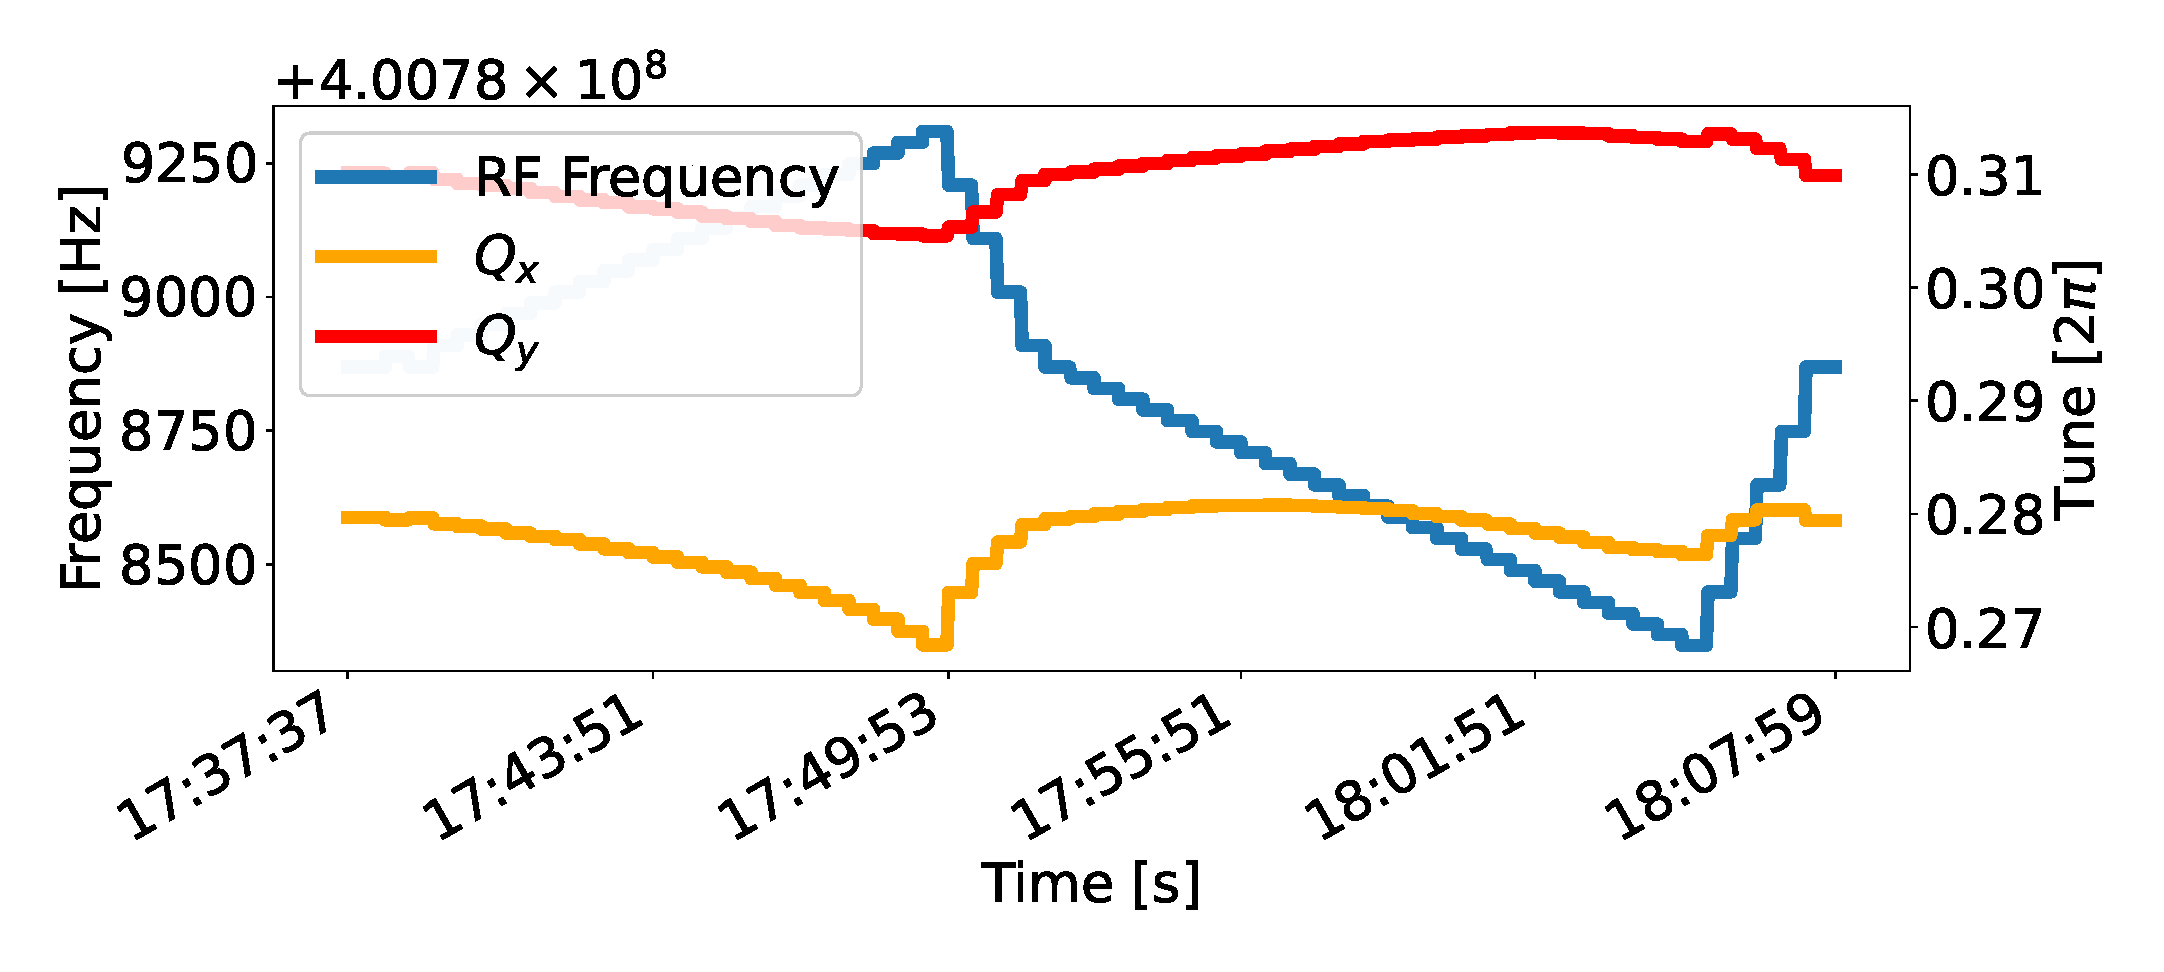
\includegraphics[width=\columnwidth]{images/MOPL027_f1-1.pdf}
%    \caption{Observation of the tune dependence on momentum offset, created by a shift of RF frequency.}
%    \label{fig:very_high_orders:rf_scan}
%\end{figure}

%To properly characterize higher orders of the chromaticity function and ensure quality measurements,
%several steps are required. The tune measured during chromaticity scans can exhibit jitter and
%resonance lines may appear, requiring thorough data cleaning to either reject problematic data
%points or reduce error bars. The simplified
%\cref{eq:very_high_orders:simplified_eq_momentum_compaction}, describing $\delta$, has been
%sufficient for reliably measuring up to the third order chromaticity. However, this relation also
%needs verification.




%------------------------------------------
%            First Measurement
%------------------------------------------
\FloatBarrier
\subsection{\review{First Observation}}

Before focusing on the measurement of higher-order chromaticity such as $Q^{(5)}$, it is essential
to consider the procedural improvements that enable such measurements. Improvements in dynamic
aperture, collimation and signal processing with noise reduction now allow for larger oscillation
amplitudes and enhancements in the precision of measurements across broader amplitude ranges. This
increased resolution facilitates the study of non-linear chromaticity, which has been extended to
include higher-order terms, making it possible to detect contributions from dodecapolar and
decatetrapolar fields.
These developments are particularly interesting because they suggest the possibility of directly
measuring $Q^{(5)}$, an observable previously inaccessible due to narrower momentum offset ranges.


A measurement was performed with the octupolar and decapolar correctors \textit{MCO} and
\textit{MCD} set to their nominal settings. These are aimed at correcting $Q''$ and $Q'''$, as
previously described in \cref{chapter:decapoles}. Results of this initial measurement are shown in
\cref{tab:high_orders:chroma_fidel}. Lower order chromaticities such as $Q'$ and $Q''$ are
consistent with measurements done during the previous Run~\cite{maclean_commissioning_2016}.
The fourth and fifth order chromaticities, $Q^{(4)}$ and $Q^{(5)}$, are primarily expected
to originate from dodecapolar errors in the quadrupoles and decatetrapolar errors in the main
dipoles, respectively, as given by the following expressions:

\begin{equation}
    \begin{aligned}
        &\Delta Q_x^{(4)} =  \frac{1}{4\pi} K_{6} L \beta_x D_x^{4}, 
        &&\Delta Q_x^{(5)} =  \frac{1}{4\pi} K_{7} L \beta_x D_x^{5},&&\\
        %
        &\Delta Q_y^{(4)} = -\frac{1}{4\pi} K_{6} L \beta_x D_x^{4},
        &&\Delta Q_x^{(5)} = -\frac{1}{4\pi} K_{7} L \beta_x D_x^{5}.
    \end{aligned}
    %\label{eq:detuning_effects:chromaticity_strength}
\end{equation}


\begin{table}[!htb]
    \centering
    \begin{tabular}{lrrrr}
    \toprule
         Plane & $Q^{(2)} [10^3]$ & $Q^{(3)} [10^6]$ & $Q^{(4)} [10^9]$ & $Q^{(5)} [10^{12}]$ \\
    \midrule
        Beam 1 &              &               &              & \\
        \hspace{2mm}X         & $-2.44 \pm 0.02$ & $-3.36 \pm 0.04$ & $-0.56 \pm 0.02 $ & $ 1.20 \pm 0.07$ \\
        \hspace{2mm}Y         & $ 0.97 \pm 0.02$ & $ 1.62 \pm 0.05$ &$  0.15 \pm 0.03$ & $-0.88 \pm 0.09$ \\
        Beam 2 &              &                &                & \\
        \hspace{2mm}X         & $-2.45 \pm 0.03$ & $-2.72 \pm 0.08$ & $-1.00 \pm 0.05 $ & $ 0.15 \pm 0.14$ \\
        \hspace{2mm}Y         & $ 0.79 \pm 0.03$ & $1.54 \pm 0.06 $ & $ 0.24 \pm 0.04 $ & $-0.74 \pm 0.13$ \\
    \bottomrule
    \end{tabular}
    \caption{Terms of the high order chromaticity obtained during Run~3's commissioning in 2022,
    with nominal corrections.}
    \label{tab:high_orders:chroma_fidel}
  \end{table}

Due to the RF-scan method, the momentum offset crosses zero multiple times during the measurement.
The absence of tune change at these points allows to conclude that the tune drift throughout
the measurement is negligible. This measurement was conducted after an extended period at
injection energy, where the decay of the sextupolar fields is minimal, causing no significant change
in first-order chromaticity. The fitted curve for the chromaticity function is shown in
\cref{fig:high_orders:chroma_before_correction}, where it is evident that a higher-order polynomial
provides a better fit.

\begin{figure}[!htb]
    \begin{subfigure}{0.49\textwidth}
        \centering
        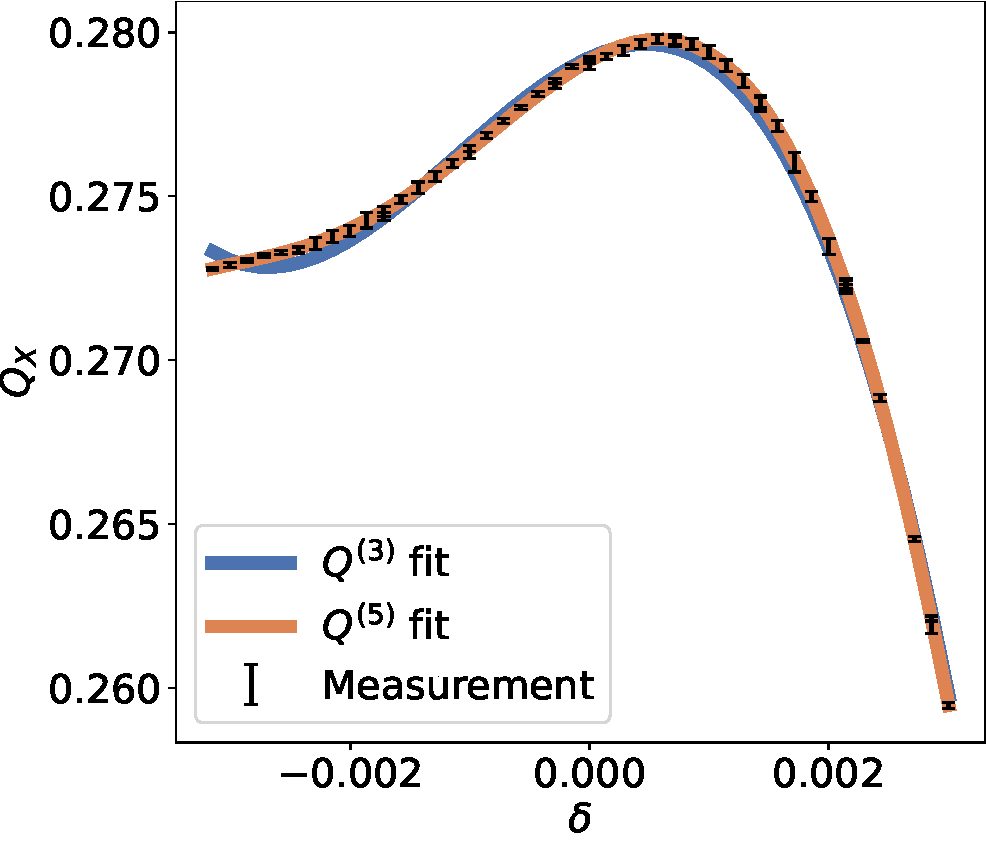
\includegraphics[width=\textwidth]{./images/higher_orders/fidel_chroma/Beam1_Qx.pdf}
        \caption{$Q_x$ Beam 1}
    \end{subfigure}
    \hfill
    \begin{subfigure}{0.49\textwidth}
        \centering
        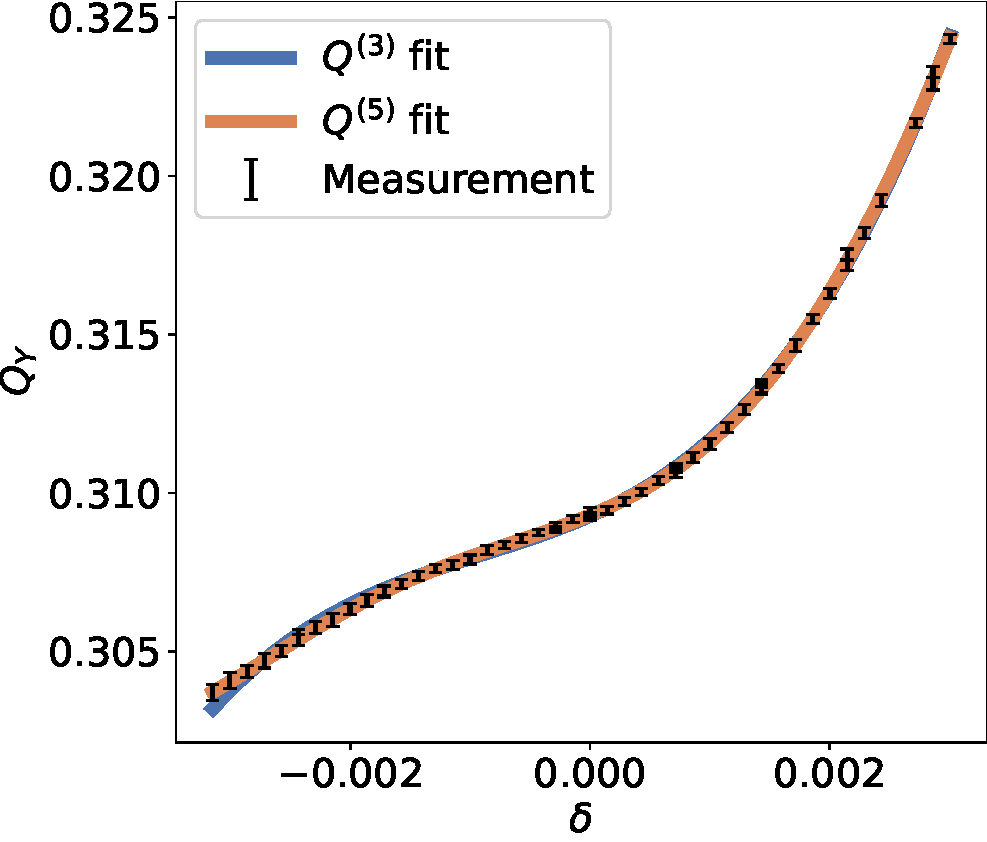
\includegraphics[width=\textwidth]{./images/higher_orders/fidel_chroma/Beam1_Qy.pdf}
        \caption{$Q_y$ Beam 1}
    \end{subfigure}
    %
    \\
    %
    \begin{subfigure}{0.49\textwidth}
        \centering
        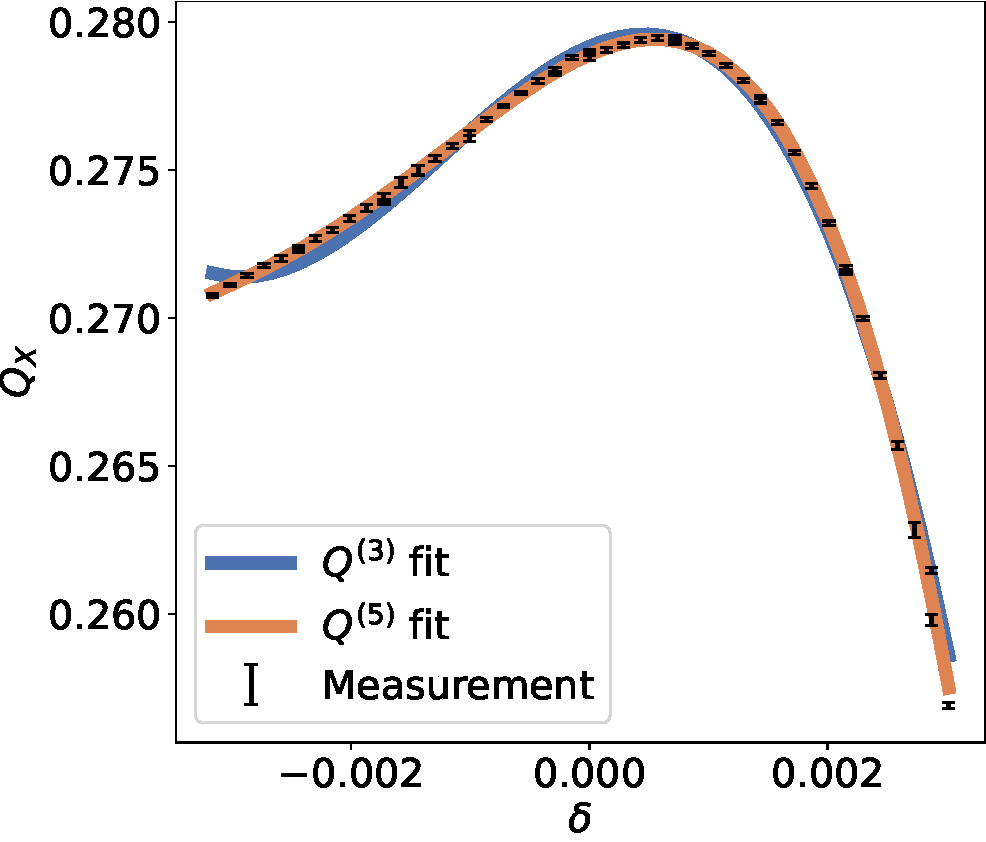
\includegraphics[width=\textwidth]{./images/higher_orders/fidel_chroma/Beam2_Qx.pdf}
        \caption{$Q_x$ Beam 2}
    \end{subfigure}
    \hfill
    \begin{subfigure}{0.49\textwidth}
        \centering
        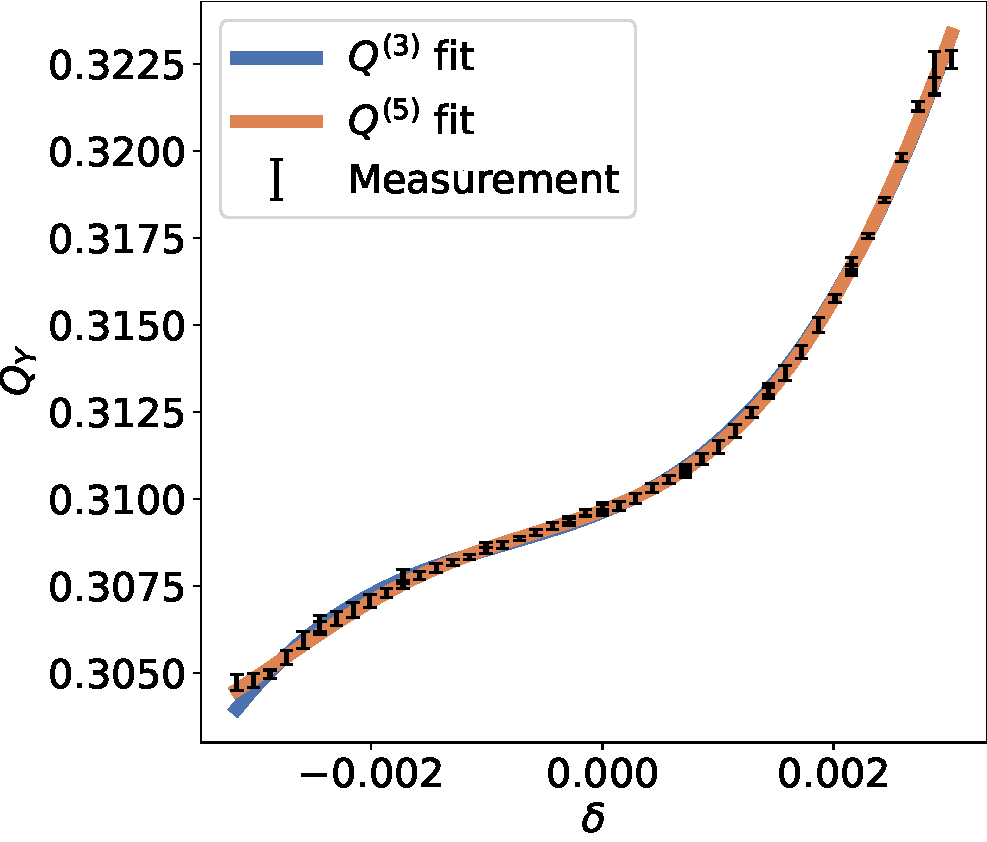
\includegraphics[width=\textwidth]{./images/higher_orders/fidel_chroma/Beam2_Qy.pdf}
        \caption{$Q_y$ Beam 2}
    \end{subfigure}
    \caption{Measurement of higher order chromaticity terms with nominal corrections used
    during operation. Fits are up to the third and fifth order.}
    \label{fig:high_orders:chroma_before_correction}
\end{figure}





%----------------------------------------
%             Fit Quality
%----------------------------------------
%\subsubsection{\review{Fit Quality}}
%\label{subsection:q4q5_quality}

%The values measured for $Q^{(4)}$ and $Q^{(5)}$ are similar across the measurements, with
%nominal and beam-based corrections performed with very different lower order chromaticity, and well 
%separated in time.
%This reproducibility with varying configurations gives confidence that the measured values are
%robust. It is to be noted that one exception exists for the first measurement, the horizontal plane
%of beam 2 showed a high correlation between the fourth and fifth order terms, making the fit less
%reliable.

The reduced chi-square for this measurement of 2022 for each fit order is detailed in
\cref{tab:high_orders:chisquare_quality}. A value of $1$ indicates a good fit. Values above indicate
a poor fit while values below show an over-fit of the data.
While adding terms to the chromaticity function is beneficial to the fit, it can be seen that the
reduced chi-square does not substantially improve above the fifth order, indicating that such
further orders are not warranted.
%\Cref{chroma_comparison} shows a comparison of the measured chromaticity before and after
%beam-based corrections for the horizontal axis of beam 1.

\begin{table}[!htb]
    \centering
    \begin{tabular}{lrrrr}
     \toprule
                  & \multicolumn{4}{c}{$\chi^2_\nu$} \\
      %\cmidrule{2-5}
        Plane     &   $Q^{(3)}$ &  $Q^{(4)}$ &   $Q^{(5)}$ &   $Q^{(6)}$  \\
      \midrule
        Beam 1    &   &   &   & \\
        % The commented out lines are from measurement with the regular BBQ data
        % The un-commented lines are from using the raw BBQ data
        %X         & 7.62  & 4.07 & 0.62 &\\             % regular
        %Y         & 0.72  & 0.57 & 0.15 &\\             % regular
        \hspace{2mm}X         & $17.9$  & $12.1$ & $1.8$ & $1.5$ \\         % raw bbq
        \hspace{2mm}Y         & $ 3.0$  & $2.2 $ & $0.7$ & $0.7 $\\          % raw bbq
        Beam 2    &    &    &   &\\
        %X         & 7.60  & 3.10 & 0.73 &\\             % regular
        %Y         & 0.48  & 0.46 & 0.16 &\\ \hline      % regular
        \hspace{2mm}X         & $17.3$ & $7.1$ & $1.8$ & $1.8$ \\           % raw bbq
        \hspace{2mm}Y         & $2.9 $ & $2.8$ & $1.0$ & $1.0$ \\            % raw bbq
      \bottomrule
    \end{tabular}
    \caption{Reduced $\chi^2$ values for each order of fit of the measured non-linear chromaticity, with $Q''$ and $Q'''$ beam-based corrections.}
    \label{tab:high_orders:chisquare_quality}
  \end{table}

%\begin{figure}[!ht]
%    \centering
%    \includegraphics[width=1\columnwidth]{images/comparison_b1x.png}
%    \caption{Comparison of the chromaticity function with nominal and beam-based corrections.}
%    \label[type]{chroma_comparison}
%\end{figure}


Given the novelty of measuring such high-order chromaticities, additional configurations were tested
to ensure the consistency of the results.
Potential sources contributing to high-order chromaticity,
such as the non-linearities of the momentum compaction factor, dispersion, coupling, or noise, are
discussed in the following sections.
Comparing the fitted chromaticity across different LHC
configurations allows to rule out potential issues stemming from the machine's specific state on the day of
measurement.



%----------------------------------------
%       Momentum Compaction Factor
\FloatBarrier
\subsubsection{\review{Momentum Compaction Factor}}
\label{subsubsection:momentum_compaction_factor_studies}

Rather than a constant, the momentum compaction factor can be expressed as an
expansion, as detailed in~\cref{subsection:coordinates_systems:momentum_compaction_factor}.
The first terms are given by the following,

\begin{equation}
    \alpha_c = 
    \underbrace{\alpha_{c,0}}_{1^\text{st} \text{ order}}
    + \underbrace{\alpha_{c,1} \delta}_{2^\text{nd} \text{ order}}
    + \underbrace{\alpha_{c,2} \delta^2}_{3^\text{rd} \text{ order}}.
\end{equation}

The expression for $\delta$, with $\alpha_c$ at the first and second order in the RF formula
(\cref{eq:very_high_orders:simplified_eq_momentum_compaction}) then reads,

\begin{equation}
    \begin{aligned}
        \delta &= -\frac{\Delta f_{RF}}{\alpha_{0} f_{RF}} && \Rightarrow \alpha_c \text{ at order 1} \\
        \delta &= \frac{- \alpha_{0} f_{RF} + \sqrt{f_{RF} 
            \left(- 4 \Delta f_{RF} \alpha_{1} + \alpha_{0}^{2} f_{RF}\right)}}{2 \alpha_{1} f_{RF}}
            && \Rightarrow \alpha_c \text{ at order 2} 
    \end{aligned}
\end{equation}

%It is assumed that only the first term is relevant as the induced difference in chromaticity is
%negligible as will be demonstrated later on.
The momentum compaction factor is computed using MADX at discrete $\delta$ values and then fitted,
as shown in \cref{fig:decapoles:chromaticity:momentum_compaction_factor}. Its non-linearity is
clearly evident. The effect of this non-linearity on the calculated $\delta$ via the RF frequency is
also presented. Field errors have not been found to have any significant impact on the $\alpha_c$
values. Previous studies indicated that the model $\alpha_c$ is consistent with the one observed in
the machine~\cite{keintzel_momentum_2021}.

\begin{figure}[!htb]
    \centering
    \begin{subfigure}[t]{0.48\textwidth}
        \centering
        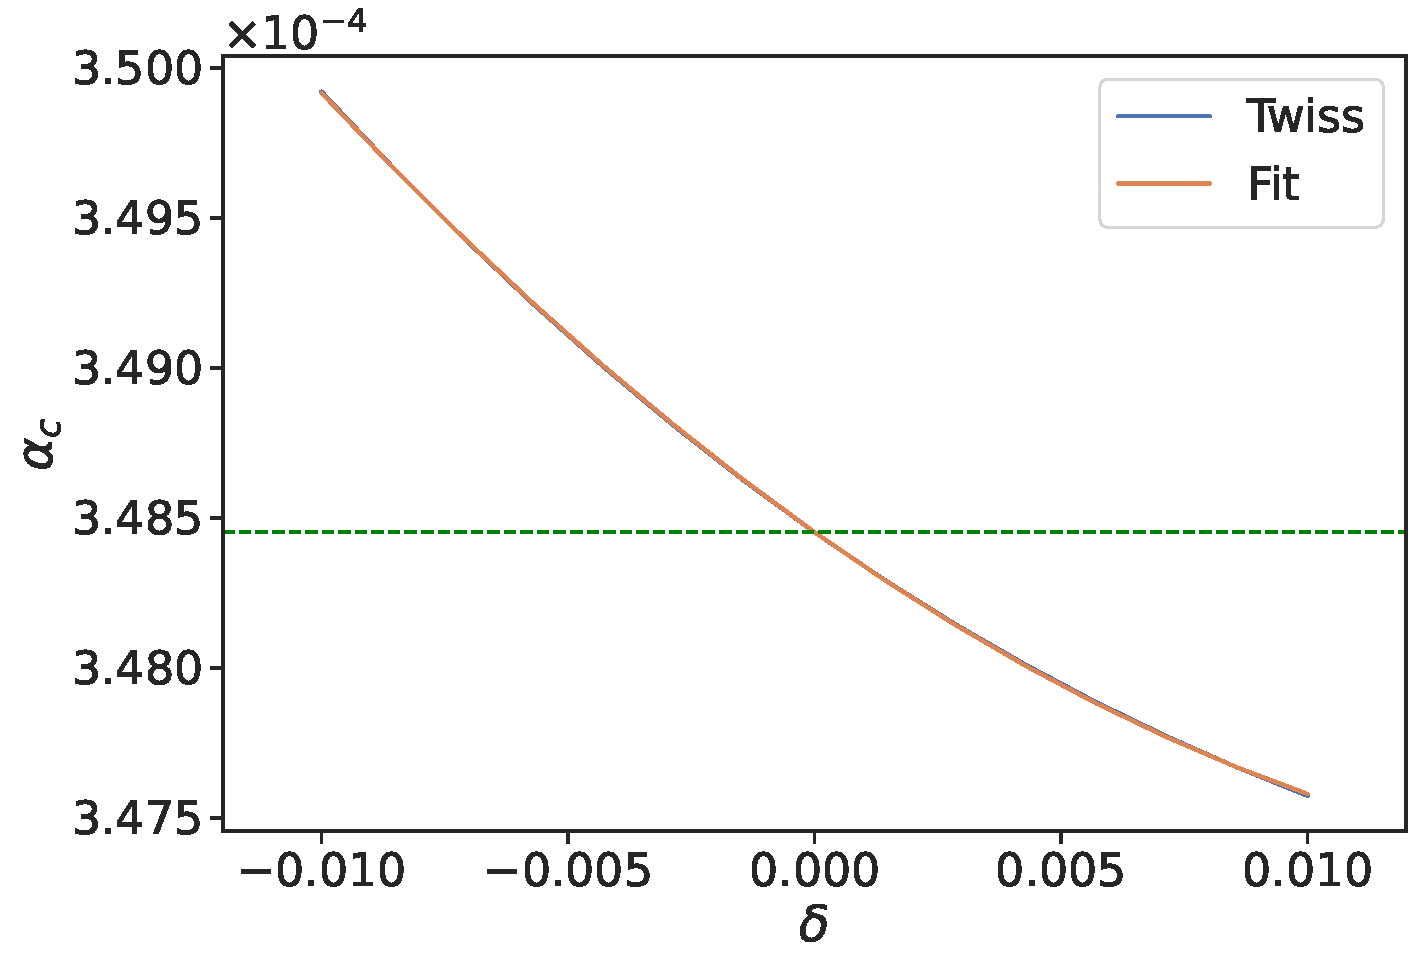
\includegraphics[width=\textwidth]{images/higher_order_momentum_compaction_factor.pdf}
        \caption{Non-linear fit of $\alpha_c$ obtained via an evaluation at discrete $\delta$ in
        MAD-X. The green line represents a constant $\alpha_c = \alpha_{c,0}$.}
    \end{subfigure}
    \hfill
    \begin{subfigure}[t]{0.48\textwidth}
        \centering
        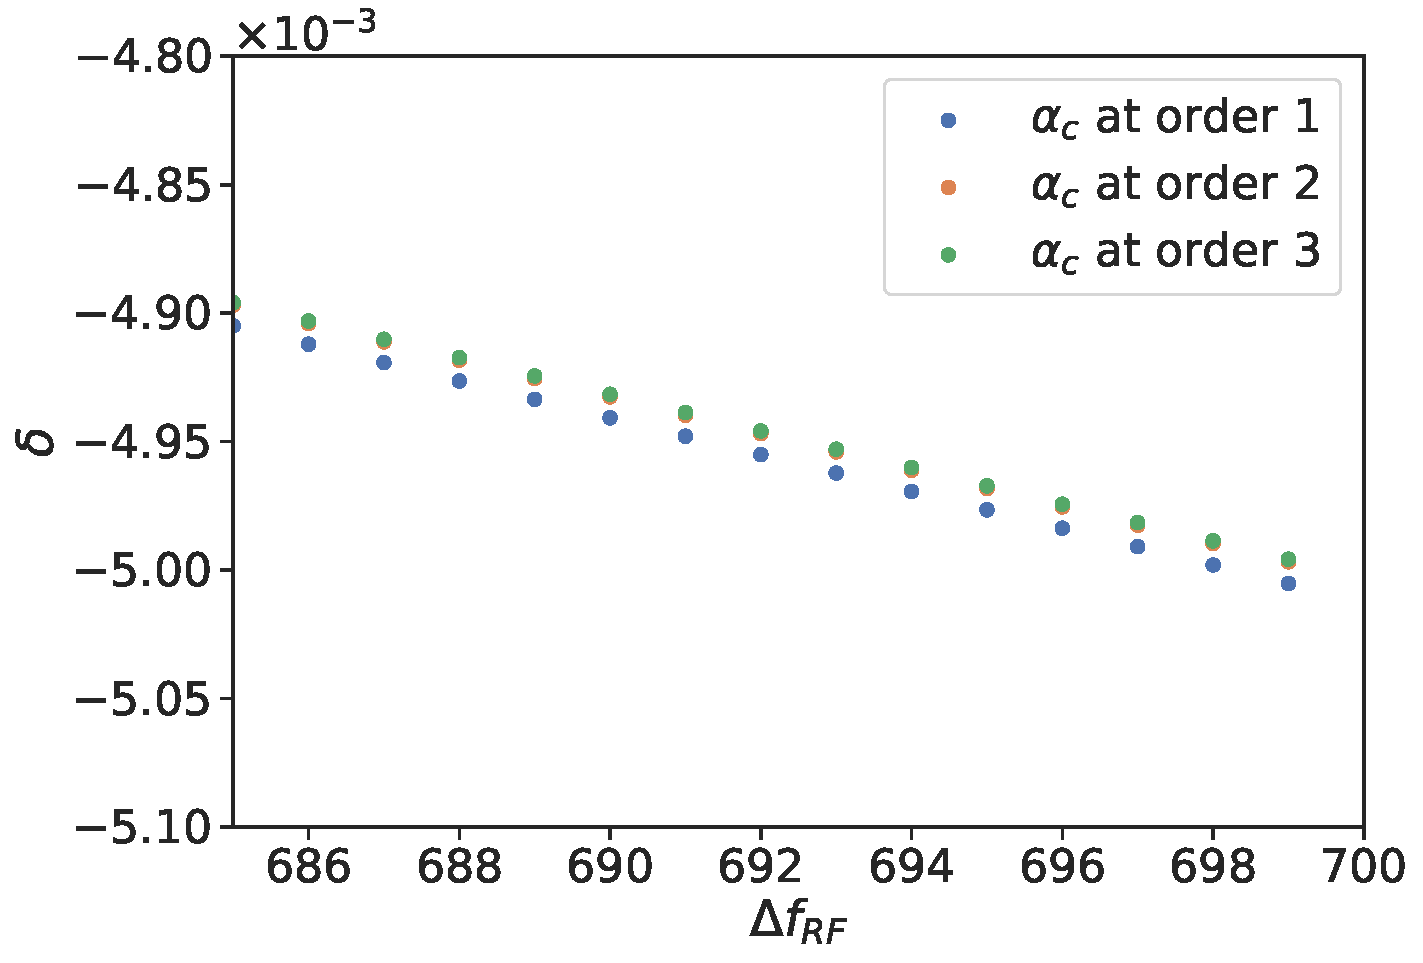
\includegraphics[width=\textwidth]{images/delta_vs_frf_alpha_c.pdf}
        \caption{Divergence of the momentum offset when considering higher $\alpha_c$ orders with
        large RF trims.}
    \end{subfigure}
    \caption{Non linearity of $\alpha_c$ and its effect on the computed $\delta$ via RF trims. The
    simulations are done at injection energy of 450 GeV.}
    \label{fig:decapoles:chromaticity:momentum_compaction_factor}
\end{figure}

It is observed that while clearly depending on higher orders, the momentum compaction factor only
has a small impact on the calculated $\delta$.
\Cref{fig:decapoles:chromaticity:momentum_compaction_factor_chroma_meas} shows a real-life 
measurement, comparing the fit of the chromaticity function with various $\delta$, computed up to
the third order of $\alpha_c$.

\begin{figure}[!htb]
    \centering
    \begin{subfigure}[t]{0.48\textwidth}
        \centering
        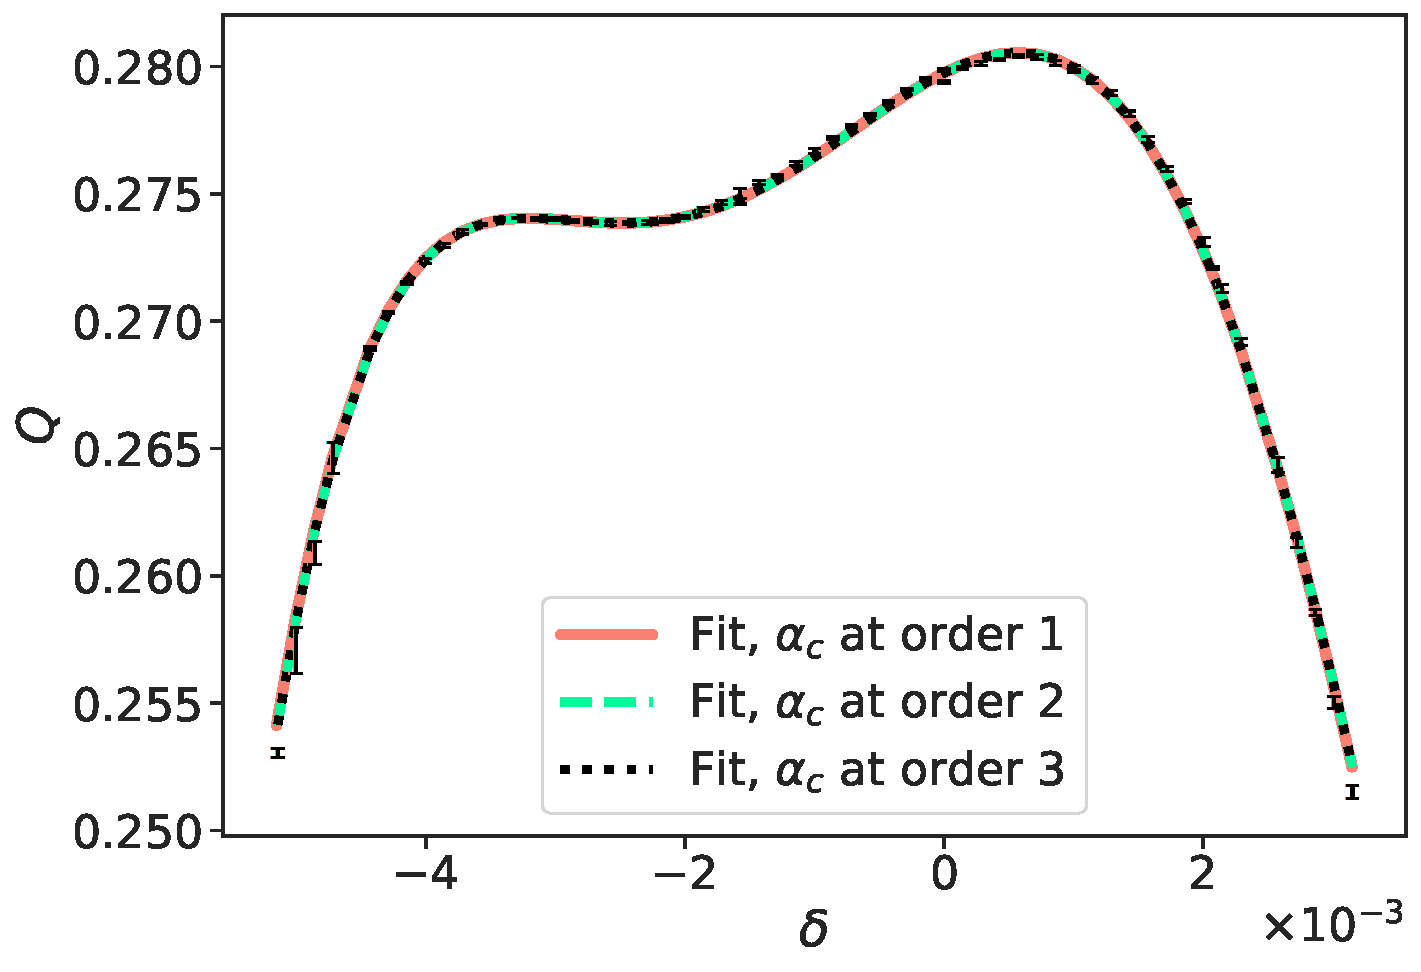
\includegraphics[width=\textwidth]{images/chroma_function_alpha_c.pdf}
        \caption{Fit of the chromaticity function at the $5^{\text{th}}$ order, considering the
        $\alpha_c$ expansion up to the third order.}
    \end{subfigure}
    \hfill
    \begin{subfigure}[t]{0.48\textwidth}
        \centering
        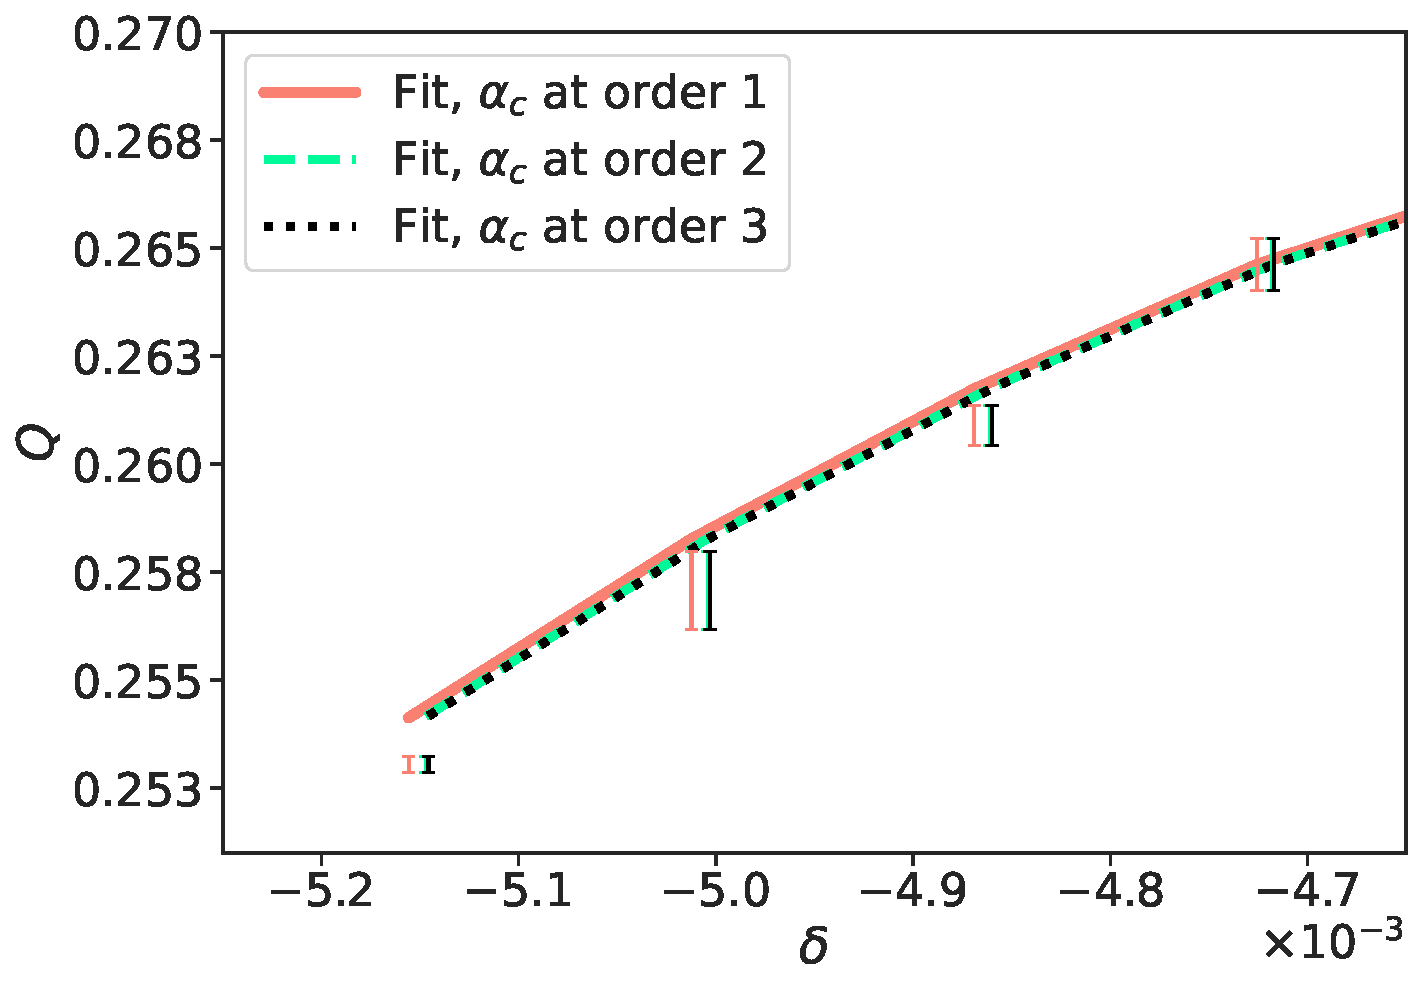
\includegraphics[width=\textwidth]{images/chroma_function_alpha_c_zoom.pdf}
        \caption{Zoom on one side of the fit. The difference between the second and third order
        is barely noticeable.}
    \end{subfigure}
    \caption{Fit of the chromaticity function considering several $\alpha_c$ orders.}
    \label{fig:decapoles:chromaticity:momentum_compaction_factor_chroma_meas}
\end{figure}

The fit of the chromaticity function is barely impacted when considering the higher orders of the 
momentum compaction factor. The different orders of the chromaticity are collected
in~\cref{table:decapoles:chromaticity:alpha_c_chroma}.
The higher order terms of $\alpha_c$ can thus be neglected and are not a source of higher
chromaticity orders.

\begin{table}[!htb]
    \centering
    \begin{tabular}{lrrr}
      \toprule
                  & \multicolumn{3}{c}{$\alpha_c$ order} \\
  %                \cmidrule{2-4}
      Chromaticity &  \multicolumn{1}{c}{1}  &  \multicolumn{1}{c}{2} &  \multicolumn{1}{c}{3} \\
      \midrule
      $Q^{(1)}$ & $ 2.52 \pm 0.03$ & $ 2.53 \pm 0.03$ & $ 2.53 \pm 0.03$ \\
      $Q^{(2)}$ & $-3.04 \pm 0.05$ & $-3.05 \pm 0.05$ & $-3.05 \pm 0.05$ \\
      $Q^{(3)}$ & $-4.75 \pm 0.03$ & $-4.75 \pm 0.03$ & $-4.75 \pm 0.03$ \\
      $Q^{(4)}$ & $-0.33 \pm 0.07$ & $-0.32 \pm 0.07$ & $-0.32 \pm 0.07$ \\
      $Q^{(5)}$ & $ 2.33 \pm 0.06$ & $ 2.36 \pm 0.06$ & $ 2.36 \pm 0.06$ \\
      \bottomrule
    \end{tabular}
    \caption{Chromaticity values obtained for the same measurement, depending on the order of the
    momentum compaction factor taken into account.}
    \label{table:decapoles:chromaticity:alpha_c_chroma}
\end{table}     



%----------------------------------------
%             Noisy Tune
\FloatBarrier
\subsubsection{\review{Noise and Spectral Lines}}

Noise lines from the electronics can be observed in the raw data obtained from the BBQ tune system.
Occasionally, when these are strong, their frequency peaks can be mistaken for the actual
tune and subsequently logged by the system. This leads to significant uncertainties in the
measurement, especially when these data points cannot be reliably classified as outliers. An example
of a tune measurement affected by this issue is shown in
\cref{fig:decapoles:chromaticity:noisy_tune}. However, this incorrect tune identification was not
problematic for measurements with narrower momentum offset ranges, as the induced tune shift was
smaller and therefore the tune less likely to overlap with strong noise lines.

\begin{figure}[!htb]
    \centering
    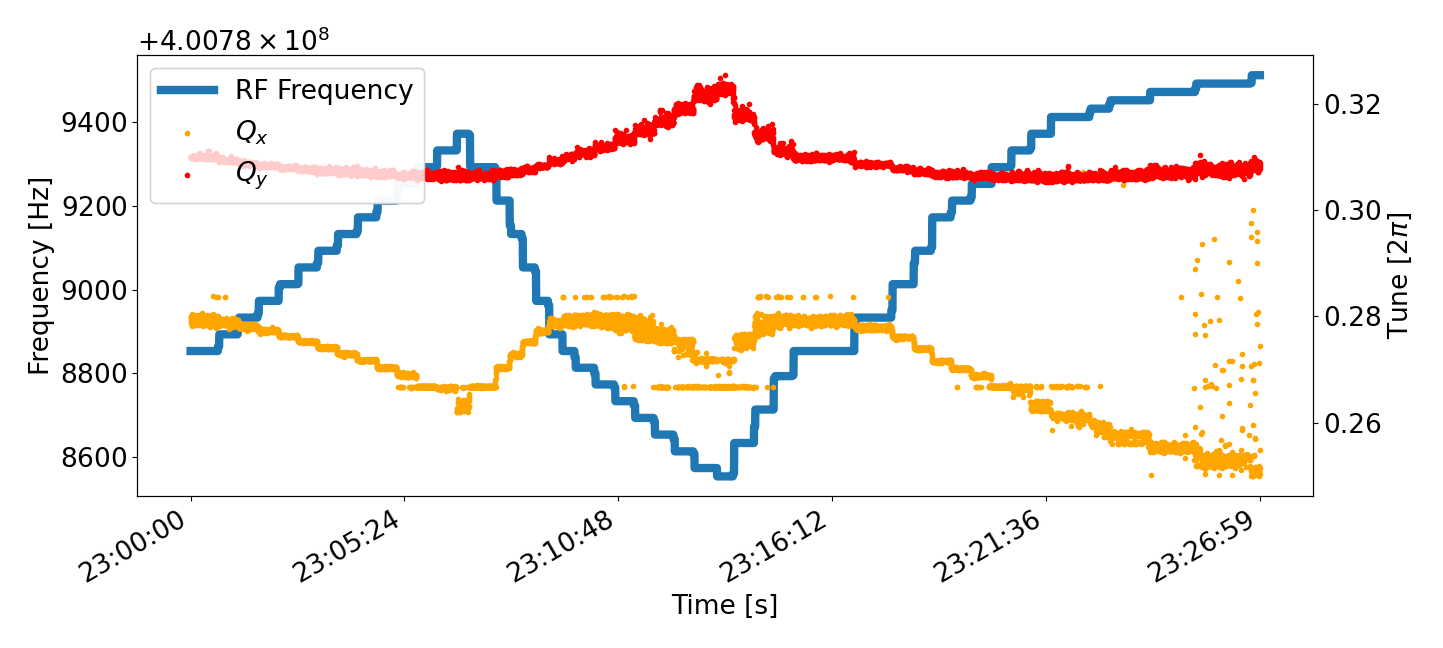
\includegraphics[width=\textwidth]{./images/noisy_tune.png}
    \caption{Shift of the tune by variation of the RF. Noise lines can appear in some cases,
    making the tune error-bar large or downright unusable.}
    \label{fig:decapoles:chromaticity:noisy_tune}
\end{figure}

A solution to this issue is to use the raw data extracted from the BBQ system. From there, a
spectrogram clearly shows the noise lines, as seen in \cref{fig:decapoles:chromaticity:spectrogram}.
Those lines have been repeatedly identified over several measurements and confirmed to be static.
The highest peak in the spectrogram can be reliably identified by removing unwanted lines,
resulting in a cleaner measurement. It is also important to note that the BBQ system requires the
tune window to be set, which, if overlooked, can lead to erroneous data. By analyzing the raw data,
it is ensured that correct data is used, preventing the measurement from inadvertently capturing
noise.

\begin{figure}[!htb]
    \centering
    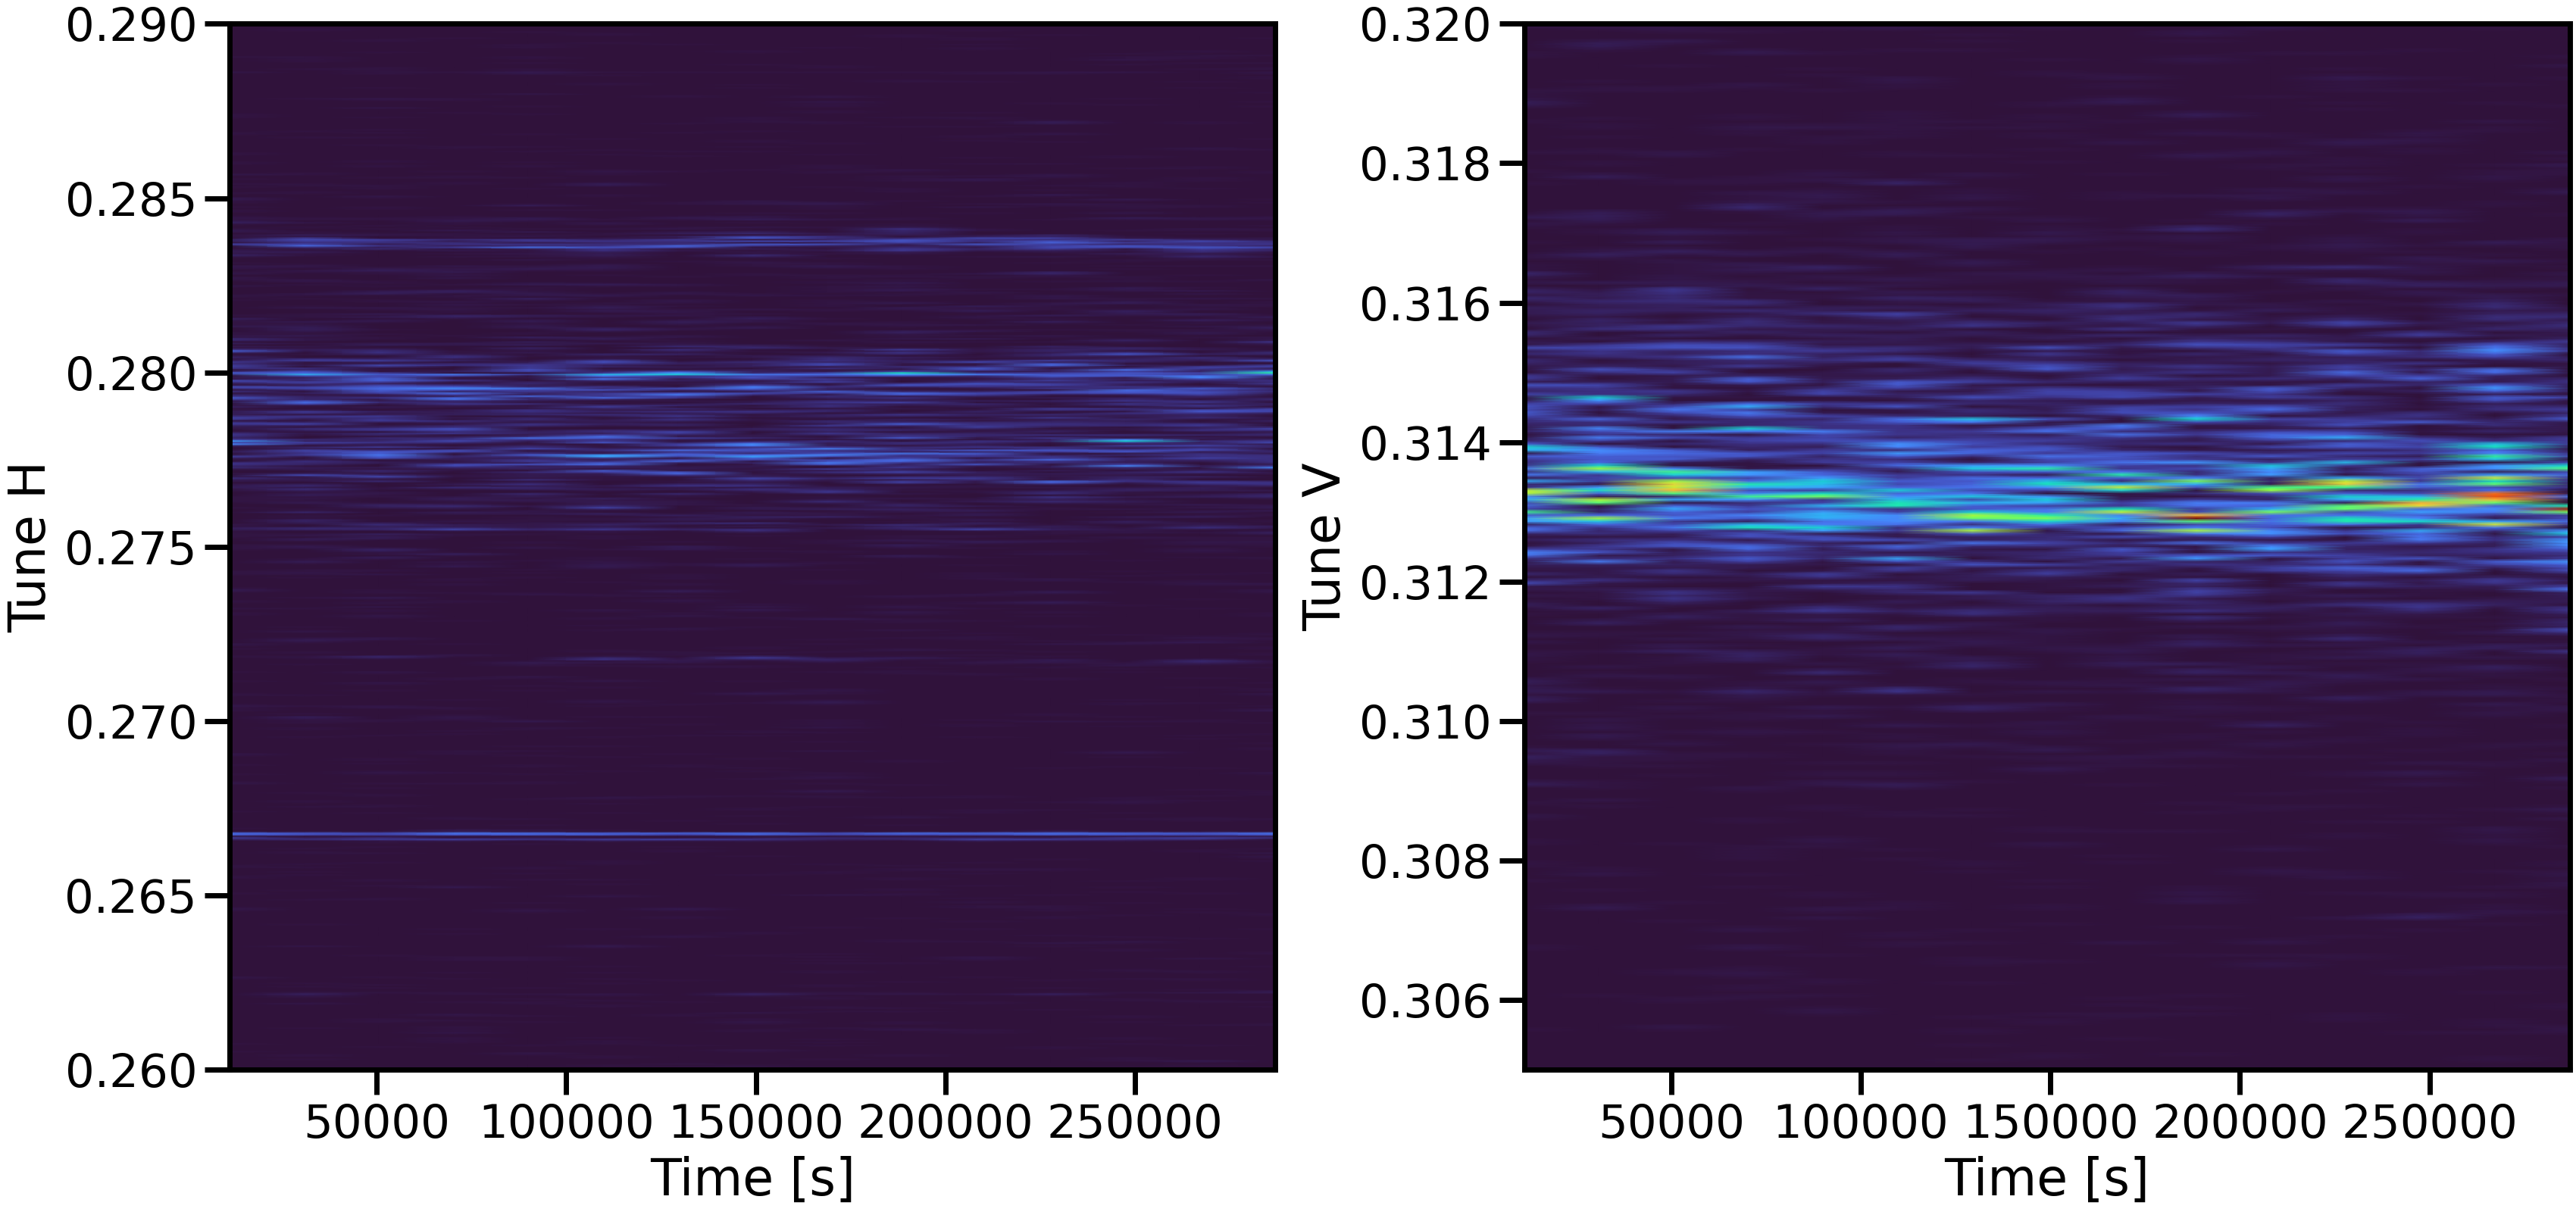
\includegraphics[width=.8\textwidth]{./images/spectrogram.png}
    \caption{Tune spectrogram obtained via the BBQ system. Strong noise lines can be seen above and
    below where the tune really is, causing the wrong frequency peak to be identified as the tune.
    These lines are always observed around $Q = 0.266$ and $Q = 0.284$}
    \label{fig:decapoles:chromaticity:spectrogram}
\end{figure}




%----------------------------------------
%         Other dpp Measurements
\FloatBarrier
\subsubsection{\review{Momentum Offset from Orbit}}

The momentum offset $\delta$ can be reconstructed through several methods. One such method,
based on beams's orbit, was previously stored by the LHC's logging services but is not
anymore. Reconstructing the momentum offset can introduce uncertainties due to the
non-linearities of both the momentum compaction factor, as discussed earlier, and the dispersion.

To evaluate this, a re-analysis of previous Run~2 measurements was conducted using the RF formula,
with the goal of comparing the resulting non-linear chromaticity values.
\Cref{fig:very_high_orders:bare_chroma_2016} shows the chromaticity measurements for Beam 1 and Beam
2 in both planes, with chromaticity computed via both the orbit-based and RF-based methods. A
numerical comparison is provided in \cref{table:very_high_orders:bare_chroma_2016}.

The lack of discrepancy between the two techniques suggests that the measurements were operating
within the linear regime of the dispersion and momentum compaction factor, and no detuning effects
were present that could have been misinterpreted as a higher-order chromaticity.

\begin{table}[!htb]
    \centering
    \begin{tabular}{lrrrr}
        \toprule
              & \multicolumn{2}{c}{$\delta$ via RF}  &  \multicolumn{2}{c}{$\delta$ via orbit} \\
        Plane & \multicolumn{1}{c}{$Q'' [10^3]$}     & \multicolumn{1}{c}{$Q''' [10^6]$} & \multicolumn{1}{c}{$Q'' [10^3]$} & \multicolumn{1}{c}{$Q''' [10^6]$}\\
        \midrule
        Beam 1 &&&& \\
        \hspace{2mm}X & $-0.64 \pm 0.01$ & $ 3.00 \pm 0.04$   & $-0.62 \pm 0.01$ & $ 2.91 \pm 0.04$ \\
        \hspace{2mm}Y & $-0.17 \pm 0.01$ & $-2.12 \pm 0.04$   & $-0.14 \pm 0.01$ & $-2.09 \pm 0.04$ \\
        Beam 2 &&&& \\
        \hspace{2mm}X & $-1.18 \pm 0.02$ & $ 2.89 \pm 0.06$   & $-1.23 \pm 0.03$ & $ 3.13 \pm 0.11$ \\
        \hspace{2mm}Y & $ 0.18 \pm 0.02$ & $-1.95 \pm 0.05$   & $ 0.20 \pm 0.02$ & $-2.02 \pm 0.06$ \\
        \bottomrule
    \end{tabular}
    \caption{Comparison of the chromaticity values obtained for the same measurement via two
    different methods to acquire $\delta$.}
    \label{table:very_high_orders:bare_chroma_2016}
  \end{table}


\begin{figure}[!htb]
    \begin{subfigure}{0.49\textwidth}
        \centering
        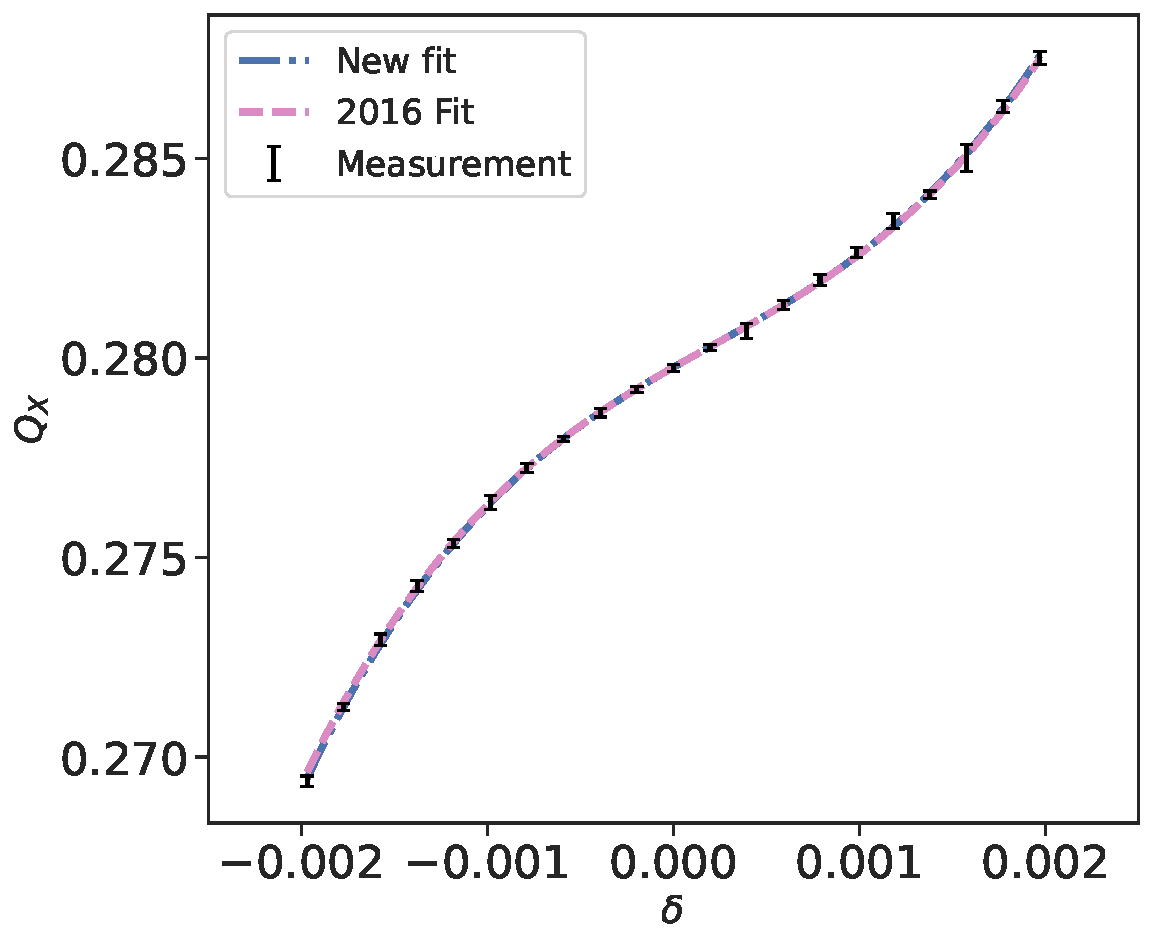
\includegraphics[width=\textwidth]{./images/chromaticity_2016/B1_qx.pdf}
        \caption{$Q_x$ Beam 1}
    \end{subfigure}
    \hfill
    \begin{subfigure}{0.49\textwidth}
        \centering
        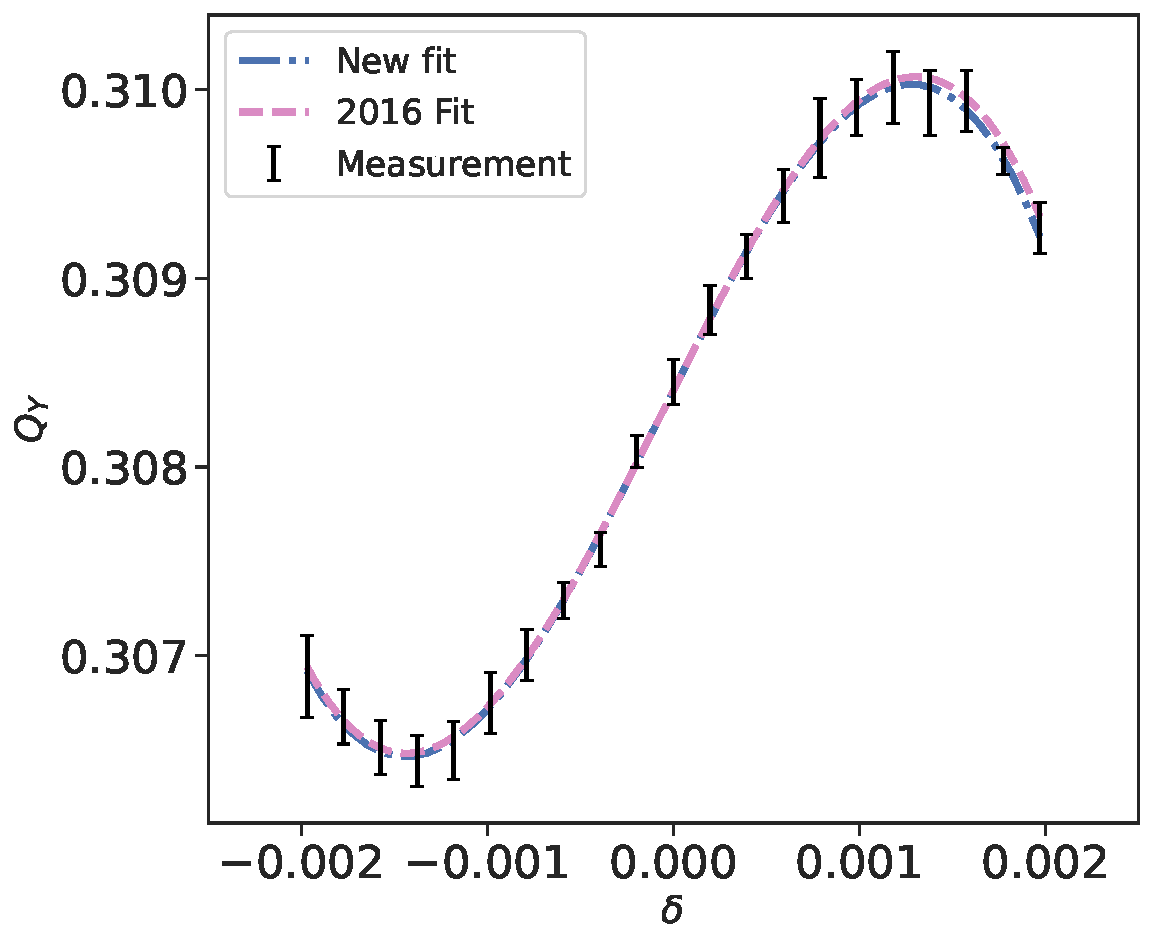
\includegraphics[width=\textwidth]{./images/chromaticity_2016/B1_qy.pdf}
        \caption{$Q_y$ Beam 1}
    \end{subfigure}
    %
    \\
    %
    \begin{subfigure}{0.49\textwidth}
        \centering
        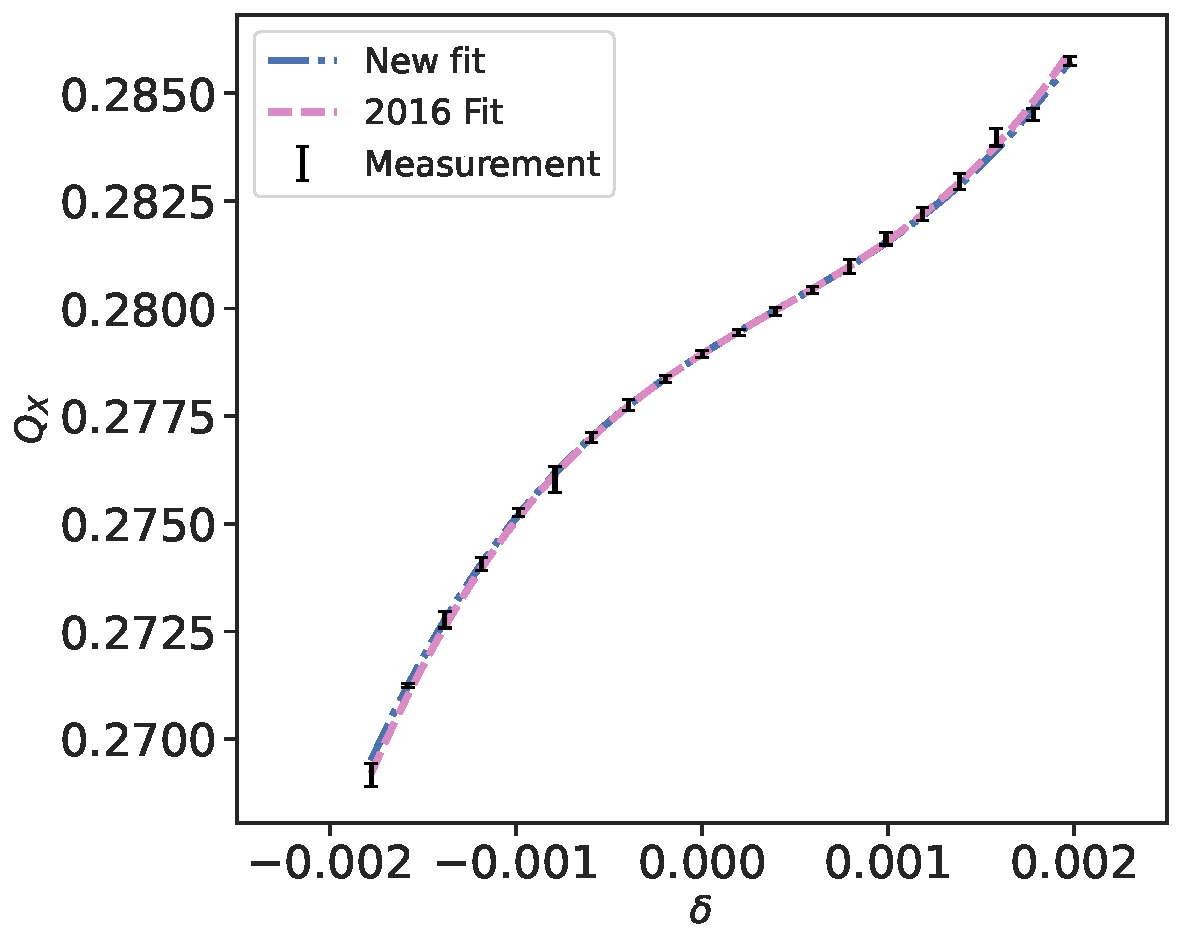
\includegraphics[width=\textwidth]{./images/chromaticity_2016/B2_qx.pdf}
        \caption{$Q_x$ Beam 2}
    \end{subfigure}
    \hfill
    \begin{subfigure}{0.49\textwidth}
        \centering
        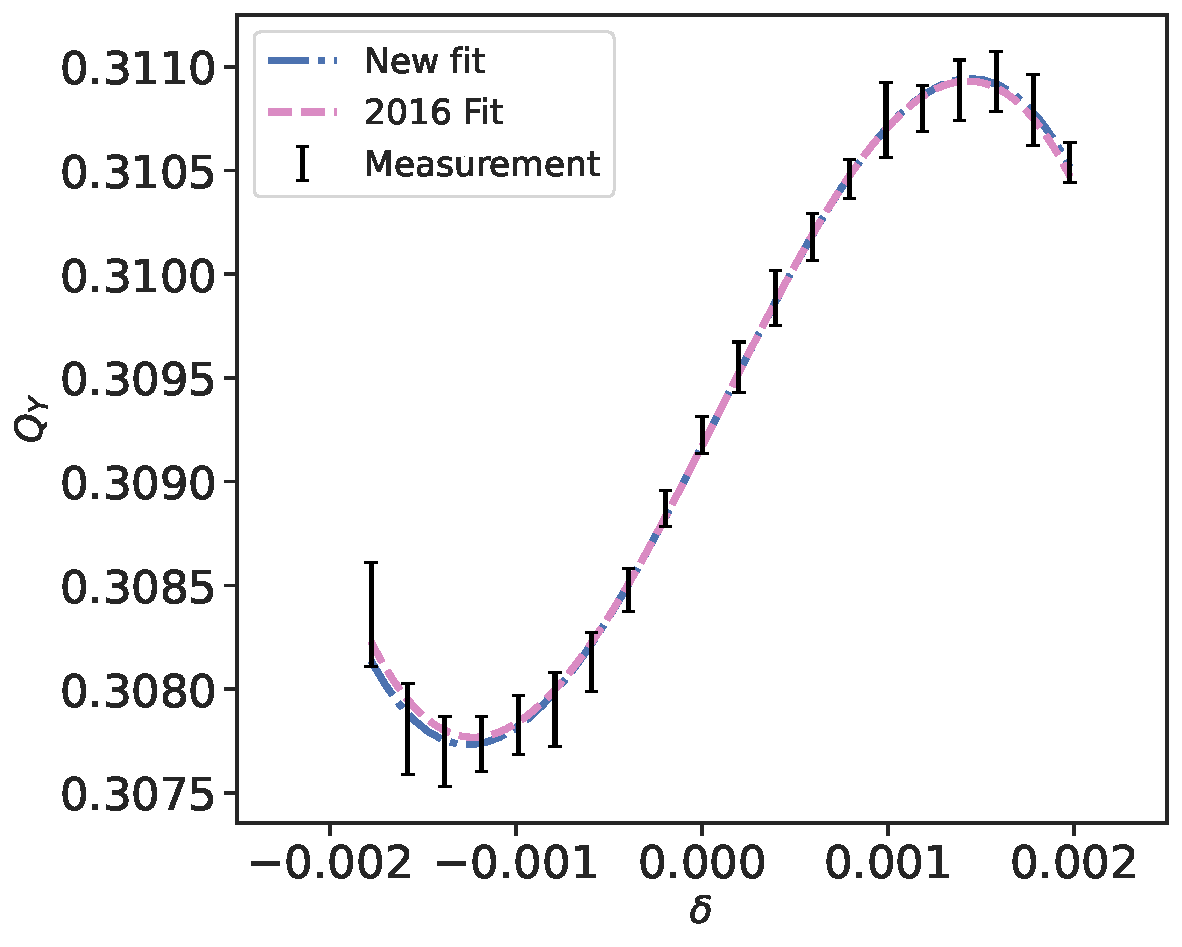
\includegraphics[width=\textwidth]{./images/chromaticity_2016/B2_qy.pdf}
        \caption{$Q_y$ Beam 2}
    \end{subfigure}
    \caption{Comparison of the non-linear chromaticity fit obtained from the computed momentum
    offset via the RF in 2022 and from the logged values in 2016.}
    \label{fig:very_high_orders:bare_chroma_2016}
\end{figure}



\FloatBarrier
%----------------------------------------
%      Other Performed Measurements
%----------------------------------------
\subsection{\review{Further Measurements}}

In order to assess the correctness of the observation of higher chromaticity orders, measurement
repeatability is needed. Two measurements were thus taken in 2022, with different configurations
pertaining to the correction of the second and third order chromaticities $Q''$ and $Q'''$. 
The first one used the nominal correction strengths for octupole and decapole corrector magnets,
derived from magnetic measurements, where the second one used beam-based corrections for the same
elements, computed from the previous measurement.
More measurements were taken during 2024's commissioning with new optics for the same reasons, to
minimize the second and third order chromaticities. Three measurements were taken: with nominal
corrections, after having corrected $Q'''$  and then $Q''$. The introduced new optics mainly changed
the powering of the triplets at the IPs and are not expected to have a considerable impact on the
chromaticity. 

\Cref{table:high_orders:dpp_ranges} shows a summary of those measurements with their respective 
achieved momentum offset ranges. While the 2024 measurements achieved greater ranges than the
previous ones, those were restricted during analysis to allow suitable comparisons.

\begin{table}[!htb]
  \centering
  \begin{tabular}{lllcc}
    \toprule
    Number & Year & Corrections      & $\delta$ min. $[\times 10^{-3}]$ & $\delta$ max. $[\times 10^{-3}]$  \\
    \midrule
    1 & 2022 & Nominal          & $-3.15$ & $3.01$  \\
    2 & 2022 & $Q''$ \& $Q'''$  & $-3.15$ & $3.72$  \\
    3 & 2024 & Nominal          & $-5.15$ & $3.15$  \\
    4 & 2024 & $Q'''$           & $-3.44$ & $4.87$  \\
    5 & 2024 & $Q''$ \& $Q'''$  & $-3.86$ & $4.44$  \\
    \bottomrule
  \end{tabular}
  \caption{Performed chromaticity measurements with their respective momentum offset ranges.}
  \label{table:high_orders:dpp_ranges}
\end{table}

In order to stay consistent, the horizontal and vertical tunes were respectively set to $Q_x = 0.28$
and $Q_y = 0.31$ for all measurements. The linear chromaticity $Q'$ is set to a small value, around
$2$, to avoid large tune shifts throughout the scan.
All measurements were performed during LHC's beam commissioning.
%, as part of the measurements and corrections performed after technical or long shutdowns.



%--------------------------------------
%       Varying Configurations
\subsubsection{\review{Varying Configurations}}

The five previously introduced measurements were performed with very different configurations for
the octupolar and decapolar correctors. \Cref{tab:high_orders:mcdo_values_corr} shows the strengths
applied on every circuit for each correction scheme, in 2022. The correction is called 
\textit{global} as all correctors are trimmed uniformly. The 2024 corrections are similar in order
of magnitude.
\Cref{fig:high_orders:comparison_2022_2024} shows the measurements and fit of some of these
measurements, to highlight their differences.

\begin{table}[H]
  \centering
  \begin{tabular}{lll}
  \toprule
    Beam  &    $K_4 [\mathrm{m}^{-4}]$      &  $K_5 [\mathrm{m}^{-5}]$  \\
  \midrule
      1   &   +3.2973    &  +1610   \\
      2   &   +2.1716    &  +1618   \\
  \bottomrule
  \end{tabular}
  \caption{Corrections applied on top of the nominal octupolar and decapolar correctors strengths in
  2022 for the $Q''$ and $Q'''$ corrections.}
  \label{tab:high_orders:mcdo_values_corr}
\end{table}

\begin{figure}[H]
  \centering
  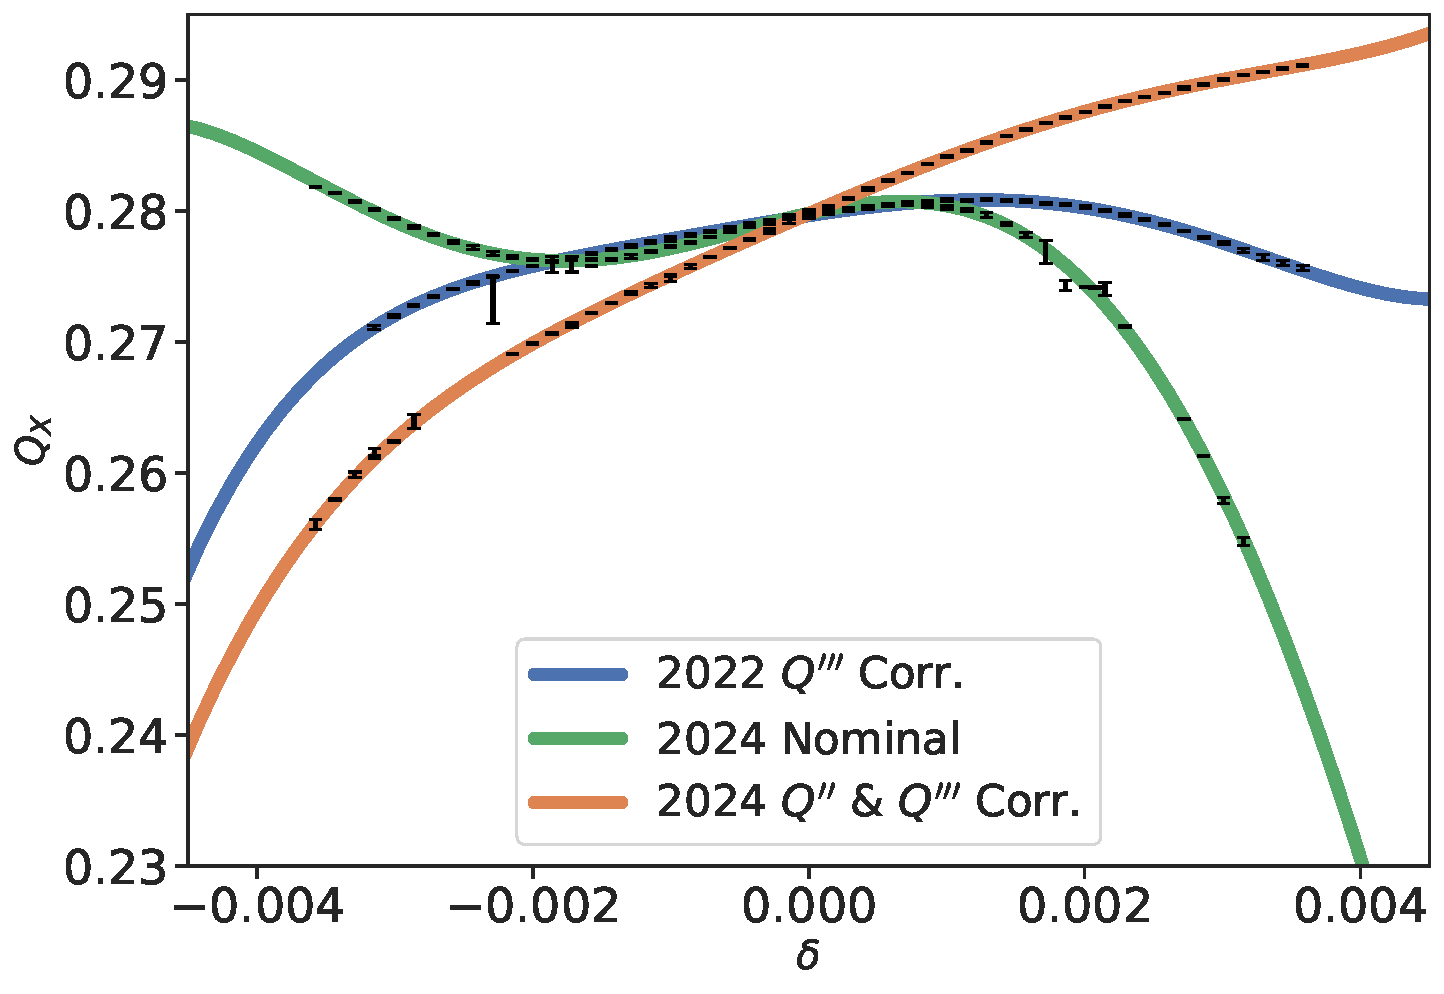
\includegraphics[width=0.7\textwidth]{./images/chromaticity_2024_vs_2022/chroma_comparison_B1_X.pdf}
  \caption{Selection of horizontal chromaticity measurements performed with varying configurations
  of the octupolar and decapolar correctors for Beam 1 during the commissionings of 2022 and 2024.}
  \label{fig:high_orders:comparison_2022_2024}
\end{figure}

A summary of the measured chromaticity orders is given in \cref{fig:high_oders:all_values}.  
The first measurement in the horizontal plane of Beam 2 suffered from low beam intensity and worse
noise, resulting in a high correlation between $Q^{(4)}$ and $Q^{(5)}$, and is therefore not included. The
last measurement for the vertical plane experienced some tune drift, making the fit impossible and
is therefore not included for both beams.

% The average is weighted by the errors
\begin{table}
  \centering
  \small
  \begin{tabular}{lrrrrr}
    \toprule
    Axis & Meas. & $Q''$ & $Q'''$ & $Q^{(4)}$ & $Q^{(5)}$ \\
    \midrule
    Horizontal &&&&&\\
    \hspace{2mm}Beam 1 & 1 & $-2.44\pm0.02$ & $-3.37\pm0.04$ & $-0.56\pm0.02$ & $ 1.21\pm0.07$ \\
                       & 2 & $-0.61\pm0.01$ & $-1.00\pm0.03$ & $-0.62\pm0.02$ & $ 1.19\pm0.05$ \\
                       & 3 & $-2.01\pm0.05$ & $-4.49\pm0.10$ & $-0.58\pm0.07$ & $ 1.34\pm0.18$ \\
                       & 4 & $-1.46\pm0.03$ & $-0.29\pm0.06$ & $-0.43\pm0.04$ & $ 1.09\pm0.10$ \\
                       & 5 & $-0.33\pm0.01$ & $-0.31\pm0.03$ & $-0.59\pm0.01$ & $ 0.75\pm0.04$ \\
                       & \textbf{Avg.}&     &                & $-0.56\pm0.07$ & $ 1.12\pm0.20$ \\%[0.5em]
                       \hdashline\noalign{\vskip 1ex}
    \hspace{2mm}Beam 2% & 1 & $-2.45\pm0.03$ & $-2.72\pm0.08$ & $-1.00\pm0.05$ & $ 0.15\pm0.14$ \\  % bad correlation for n°1
                       & 2 & $-0.85\pm0.01$ & $-0.66\pm0.03$ & $-0.57\pm0.02$ & $ 1.09\pm0.06$ \\
                       & 3 & $-2.93\pm0.05$ & $-4.40\pm0.08$ & $-0.53\pm0.08$ & $ 1.66\pm0.16$ \\
                       & 4 & $-2.21\pm0.02$ & $-0.00\pm0.03$ & $-0.46\pm0.02$ & $ 1.18\pm0.05$ \\
                       & 5 & $-0.53\pm0.02$ & $-0.09\pm0.03$ & $-0.57\pm0.02$ & $ 0.98\pm0.05$ \\
                       & \textbf{Avg.}&     &                & $-0.53\pm0.04$ & $ 1.23\pm0.26$ \\%[0.5em]
                       \midrule
    Vertical &&&&&\\
    \hspace{2mm}Beam 1 & 1 & $ 0.97\pm0.02$ & $ 1.62\pm0.05$ & $ 0.15\pm0.03$ & $-0.88\pm0.09$ \\
                       & 2 & $-0.23\pm0.01$ & $ 0.13\pm0.02$ & $ 0.09\pm0.02$ & $-0.60\pm0.03$ \\
                       & 3 & $ 0.83\pm0.02$ & $ 1.97\pm0.03$ & $ 0.29\pm0.02$ & $-0.68\pm0.05$ \\
                       & 4 & $ 0.62\pm0.01$ & $-0.18\pm0.03$ & $ 0.00\pm0.02$ & $-0.56\pm0.05$ \\
                       %& 5 & $-0.28\pm0.02$ & $-0.25\pm0.04$ & $ 0.28\pm0.02$ & $-0.12\pm0.05$ \\
                       & \textbf{Avg.}&     &                & $ 0.13\pm0.11$ & $-0.68\pm0.12$ \\%[0.5em]
                       \hdashline\noalign{\vskip 1ex}
    \hspace{2mm}Beam 2 & 1 & $ 0.79\pm0.03$ & $ 1.54\pm0.06$ & $ 0.24\pm0.04$ & $-0.74\pm0.13$ \\
                       & 2 & $-0.29\pm0.01$ & $ 0.10\pm0.02$ & $ 0.13\pm0.02$ & $-0.58\pm0.04$ \\
                       & 3 & $ 0.89\pm0.02$ & $ 2.05\pm0.03$ & $ 0.32\pm0.03$ & $-0.73\pm0.06$ \\
                       & 4 & $ 0.60\pm0.02$ & $-0.14\pm0.03$ & $ 0.04\pm0.02$ & $-0.66\pm0.05$ \\
                       %& 5 & $-0.62\pm0.02$ & $-0.29\pm0.04$ & $ 0.29\pm0.02$ & $-0.19\pm0.06$ \\
                       & \textbf{Avg.}&     &                & $ 0.18\pm0.11$ & $-0.68\pm0.06$ \\%[0.5em]
    \bottomrule
  \end{tabular}
  \caption{Summary of the chromaticity values obtained from the measurements presented in
  \cref{table:high_orders:dpp_ranges}.}
  \label{fig:high_oders:all_values}
\end{table}

The consistent identification of fourth and fifth order chromaticity across various configurations
of the LHC, with differing lower order chromaticity and coupling, enhances confidence in their
identification. Previous studies have typically focused on fits limited to the third order. However,
expanding the analysis to include fifth order not only increases the estimate of $Q'''$ but also
enhances the overall fit quality. Accurately measuring third order chromaticity is crucial for its
correction, underscoring the importance of considering higher order terms.


\FloatBarrier
%----------------------------------------
%            Model Estimates
%----------------------------------------
\subsection{\review{Model Estimates}}
\label{sec:nl_chroma_model}

Benchmarking the magnetic model of the LHC is important, in order to gauge its correctness and that
of the error tables in use, and address any potential discrepancies. The model of the LHC is based on
MADX and magnetic field error tables~\cite{p_hagen_wise_2006}, containing seeds for the random
errors. To compute the chromaticity, simulations are run via PTC, with a selection of these field 
errors.

Simulations incorporating various field errors have been conducted to evaluate the contributions of
individual magnet orders to fourth and fifth order chromaticity. Field errors
are applied to all magnets, with $b_2$ errors in the main dipoles resulting in a $\beta$-beating of
approximately $10\%$. Coupling is introduced using global knobs to create a $C^-$ value of $0.001$,
which is commonly observed during operation. Normal and skew field errors, ranging from sextupolar
($b_3$) to decahexapolar ($b_8$), are added either individually or in combination to determine which
has the strongest effect.


% ----------------------------------
\paragraph{\review{Fourth Order Chromaticity}}

The results from simulations strongly imply that the dodecapolar errors are the main contributors
to $Q^{(4)}$, as can be seen in \cref{fig:high_orders:beam1_q4_ptc}.
The most notable effect on this chromaticity order is the beta-beating, introducing a very large
spread via the various error seeds.
Comparing the simulation at the top with most errors added, the $b_6$ component alone accounts for
$\approx 70\%$ of it for both axes on each beam.

\begin{figure}[!htb]
    \centering
    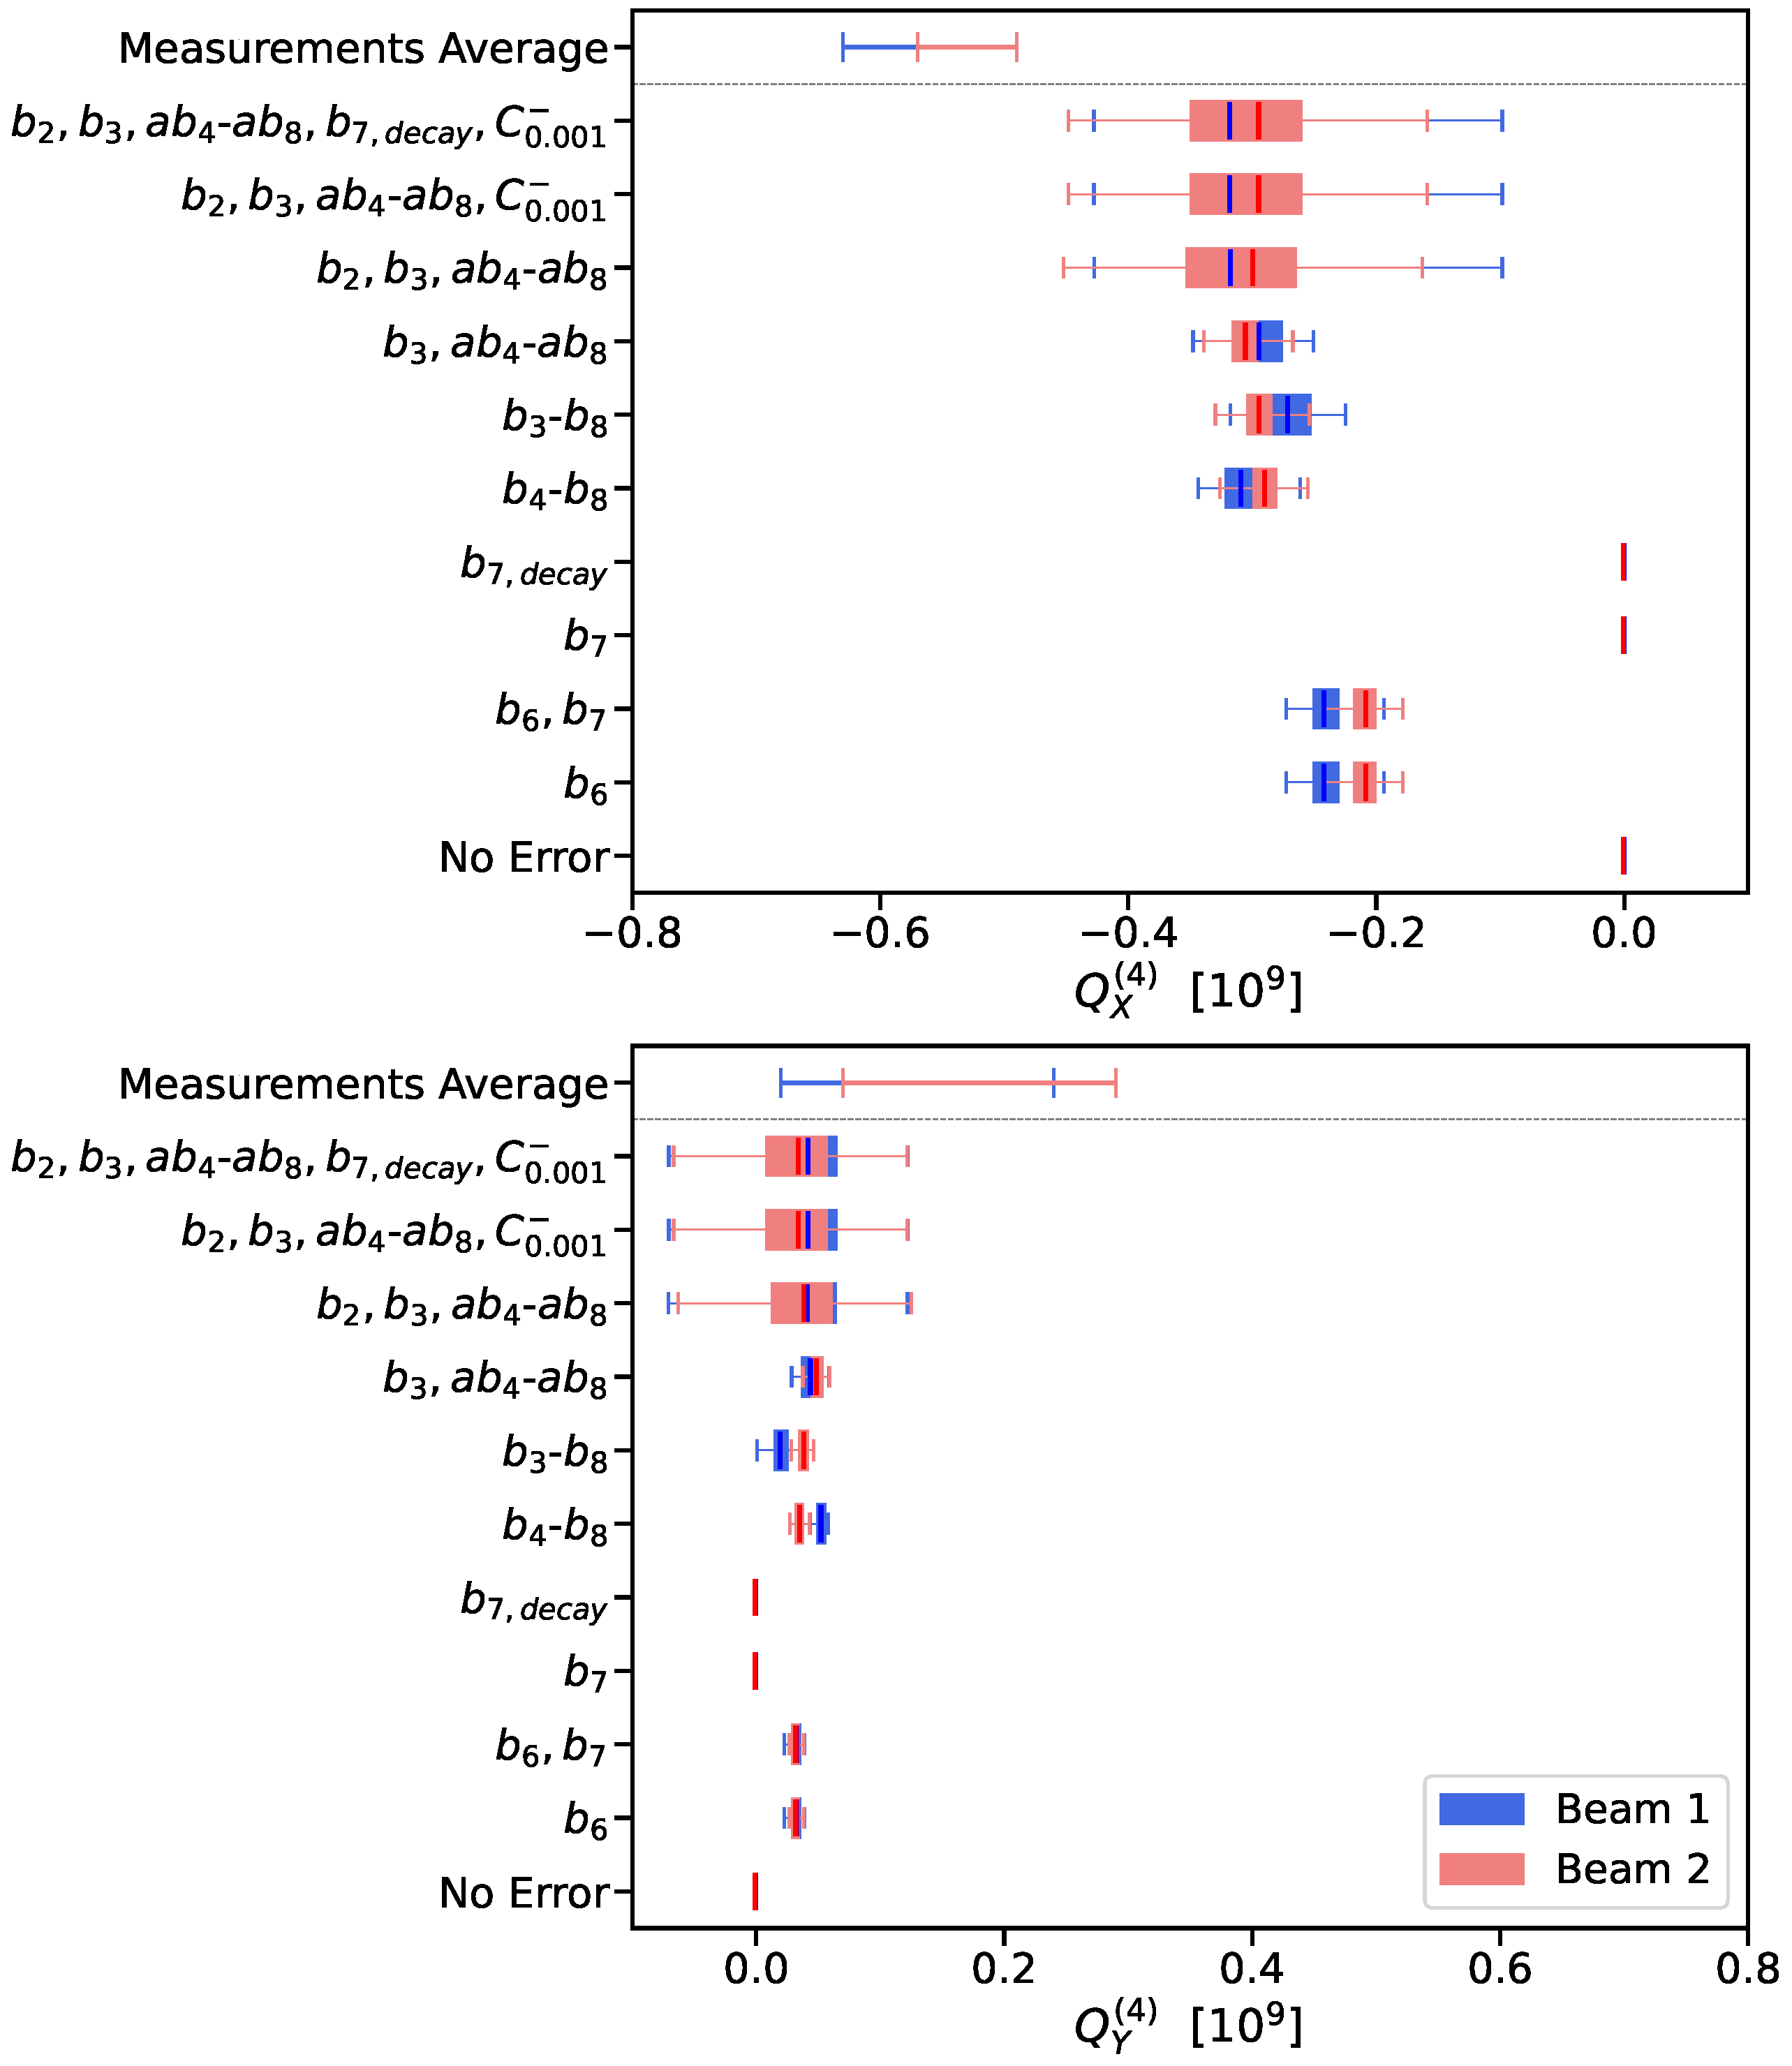
\includegraphics[width=0.9\columnwidth]{images/q4_ptc.pdf}
    \caption{Measured and simulated fourth order chromaticity with different multipole errors. The
    $b_2$ errors, applied on dipoles and quadrupoles, generate beta-beating. Coupling is set to a
    value commonly seen in operation.}
    \label{fig:high_orders:beam1_q4_ptc}
\end{figure}



% ----------------------------------
%\FloatBarrier
\paragraph{\review{Fifth Order Chromaticity}}

It is seen that the the decatetrapolar errors are the main contributors to $Q^{(5)}$, as can be seen
in \cref{fig:high_orders:beam1_q5_ptc}. Fringe fields and skew multipoles have been found to have a
negligible impact. 
Beta-beating and coupling are seen to increase by a small amount the chromaticity, while sextupolar
errors induce a spread with the different seeds. 
Comparing the simulation at the top with most errors added, the $b_7$ component alone accounts for
$\approx 70\%$ of it for both axes on each beam.

\begin{figure}[!htb]
    \centering
    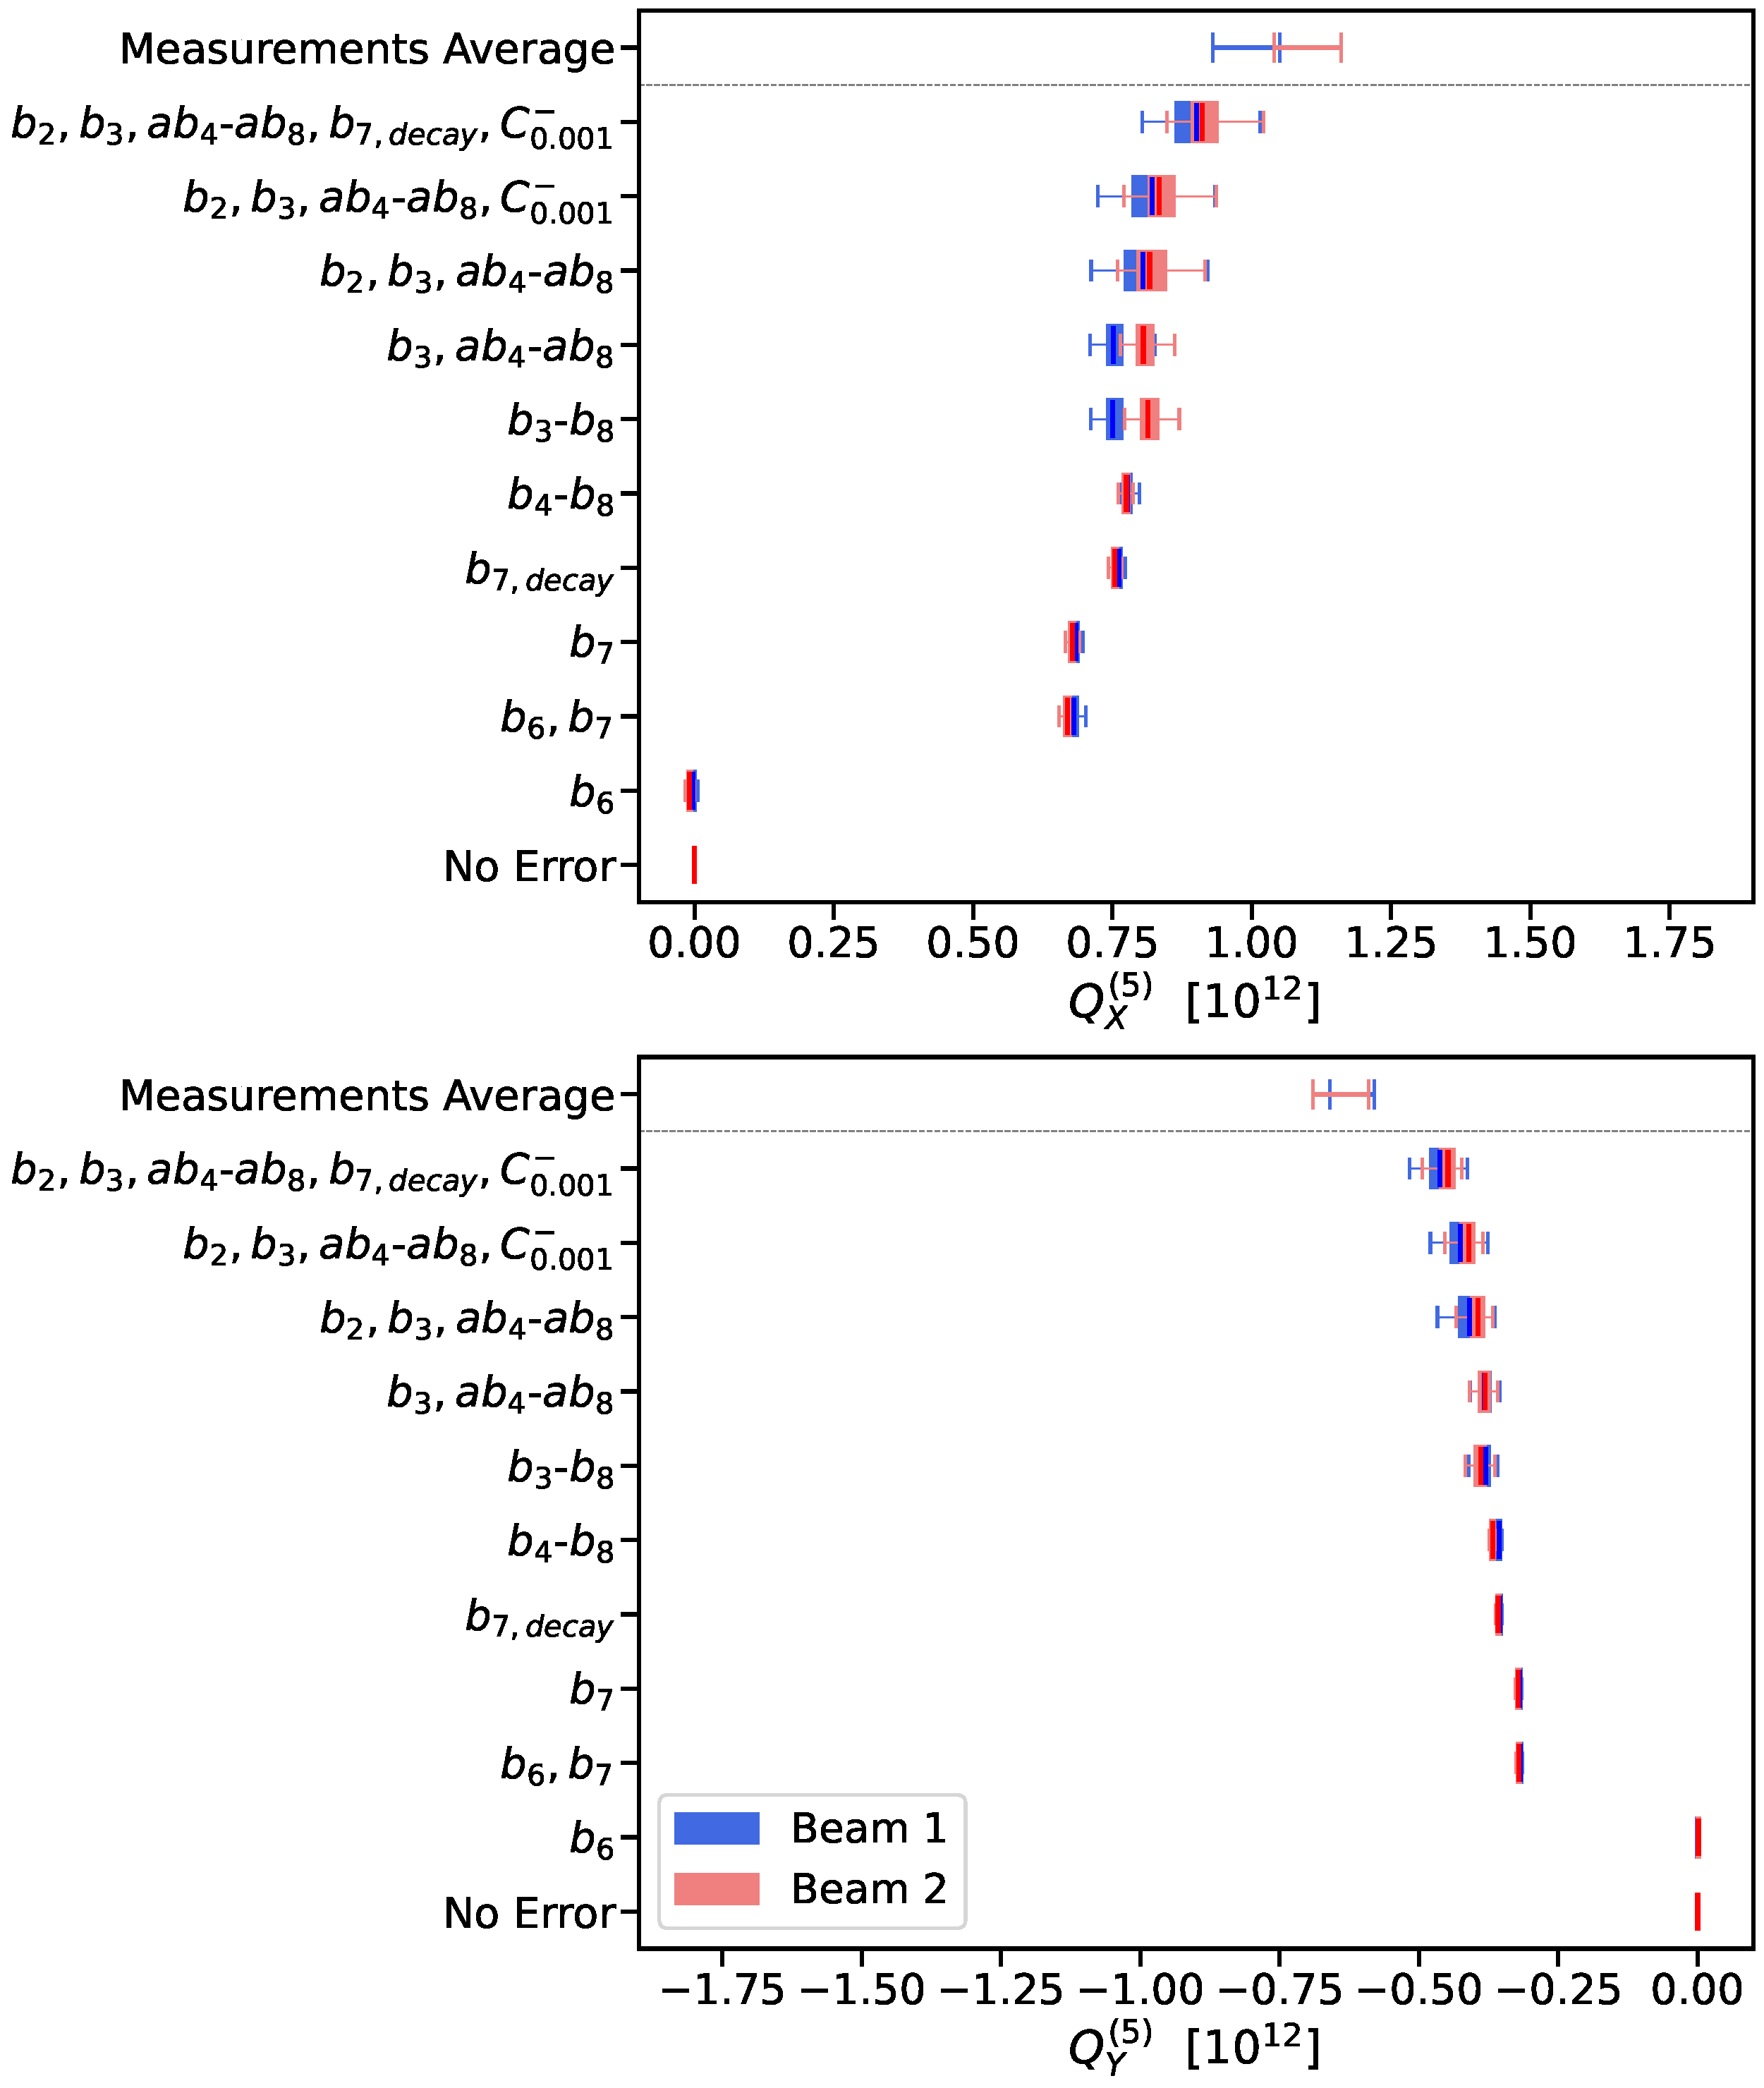
\includegraphics[width=0.9\columnwidth]{images/q5_ptc.pdf}
    \caption{Measured and simulated fifth order chromaticity with different multipole errors. The
    $b_2$ errors, applied on dipoles and quadrupoles, generate beta-beating. Coupling is set to a
    value commonly seen in operation.}
    \label{fig:high_orders:beam1_q5_ptc}
\end{figure}


% Decay
It has been noted in the previous chapter about decapoles (see \cref{section:decapoles:decay}) that
the $b_5$ component in the main dipoles was large at injection energy, and could explain most of the
discrepancy between the measurements and simulations.
Such a decay in the main dipoles also exists for the $b_7$ component~\cite{deniau2024private}, and
is shown in \cref{fig:high_orders:b7_decay}. 

\begin{figure}[!htb]
    \centering
    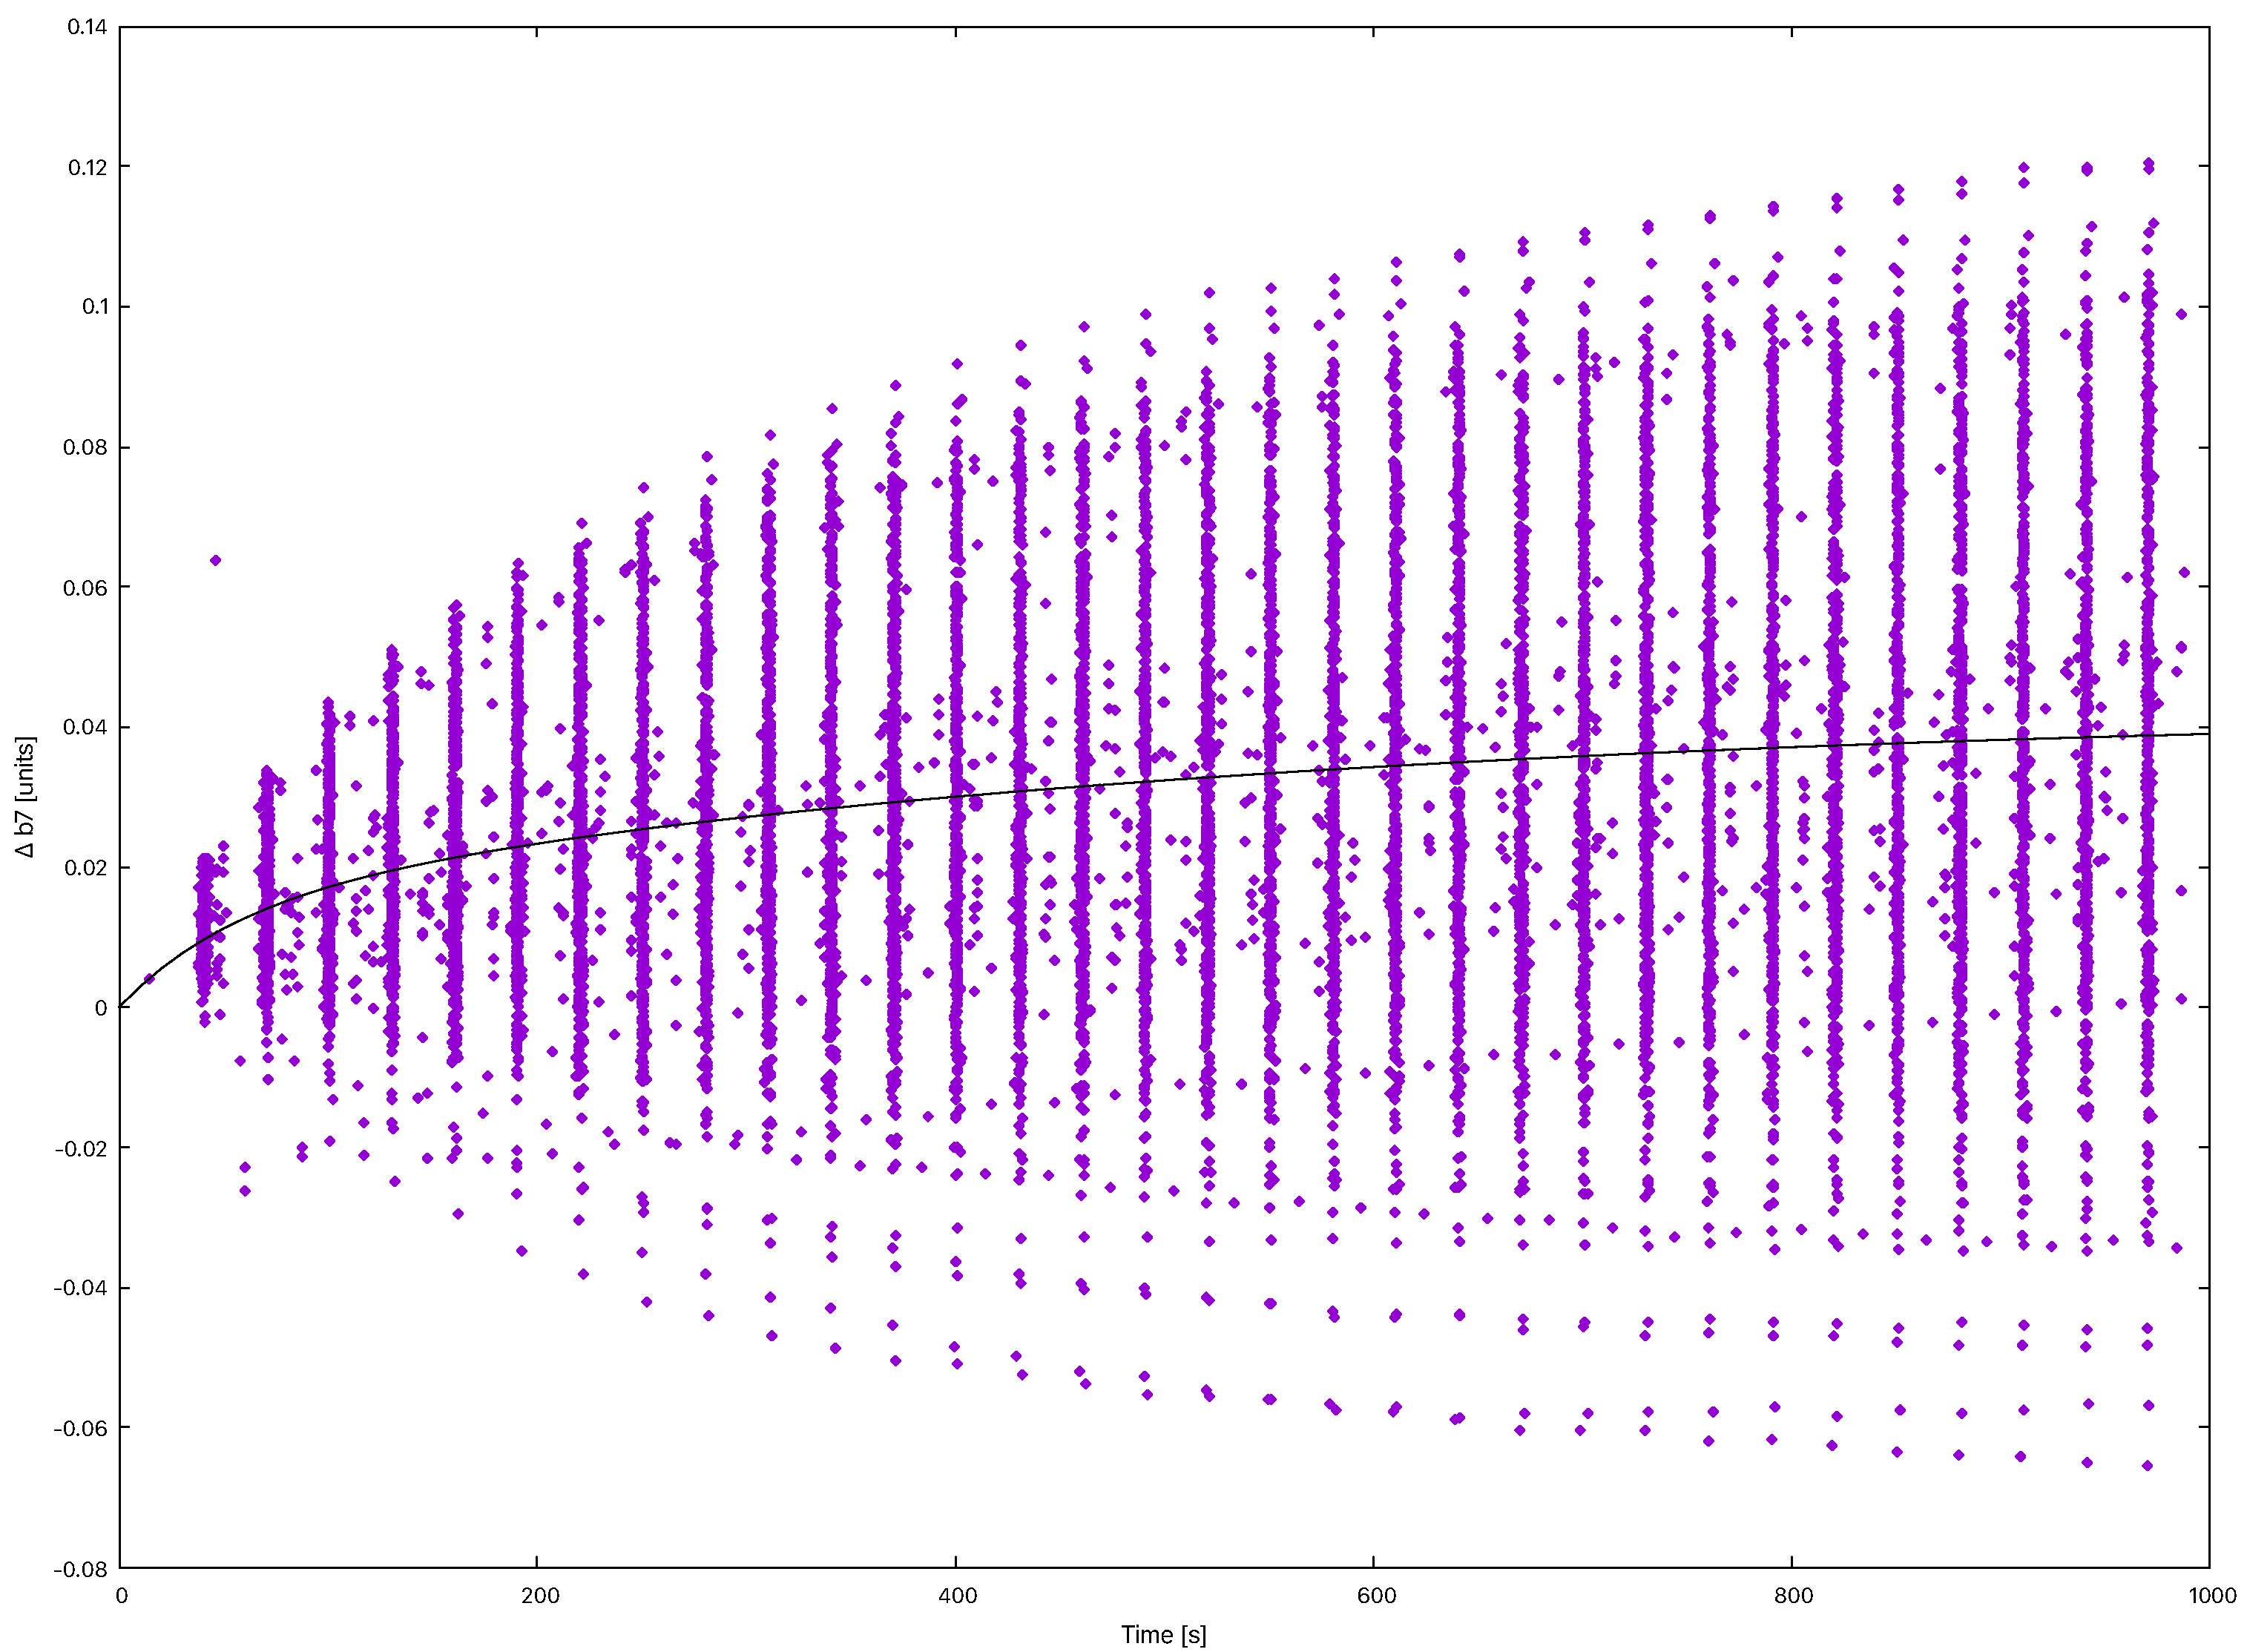
\includegraphics[width=0.9\columnwidth]{images/decay_b7.pdf}
    \caption{Measured decay of the integrated decatetrapolar field in LHC's main dipoles at
    injection energy. The fit is shown in black~\cite{deniau2024private} and settles around
    $+0.035$.}
    \label{fig:high_orders:b7_decay}
\end{figure}

Its value is though small and settles around $+0.0351 \pm 0.0007$. The average $b_7$ of the main
dipoles is of $0.32 \pm 0.16$. The decay thus increase that value of only about $11\%$.
Simulations done with that decay taken into account are also present in the previous
\cref{fig:high_orders:beam1_q5_ptc}.


%----------------------------------------
%       Agreement with Measurements
\FloatBarrier
\subsubsection{\review{Agreement with Measurements}}

Previous simulation results are shown in \cref{tab:high_orders:ptc_values}, taking the values from 
the simulation including the most effects at the top of the plots. For the fourth order, the beating
is not included as the large induced $Q^{(4)}$ is not yet explained.
\Cref{tab:high_orders:ptc_values_ratios} shows the ratio between the measured average and simulated
chromaticities.

\begin{table}[!htb]
  \centering
  \begin{tabular}{lrr}
  \toprule
      Plane     &  $Q^{(4)} [10^9]$  &  $Q^{(5)} [10^{12}]$ \\
  \midrule
      Beam 1    &              &               \\
      \hspace{2mm}X         & $-0.29 \pm 0.02$ & $ 0.90 \pm 0.05$  \\
      \hspace{2mm}Y         & $ 0.04 \pm 0.01$ & $-0.46 \pm 0.03$  \\
      Beam 2    &  &   \\
      \hspace{2mm}X         & $-0.31 \pm 0.02$ & $ 0.92 \pm 0.03$ \\
      \hspace{2mm}Y         & $ 0.05 \pm 0.00$ & $-0.45 \pm 0.01$ \\
  \bottomrule
  \end{tabular}
  \caption{Simulated high order chromaticity terms via PTC at injection energy, including normal and
  skew sextupolar to decahexapolar field errors. Are also included beta-beating, coupling and
  decatetrapolar decay. For the fourth order, the values do not include beta-beating as the observed
  spread is not yet fully understood.}
  \label{tab:high_orders:ptc_values}
\end{table}

%\begin{table}[!htb]
%  \centering
%  \footnotesize
%  \begin{tabular}{lcccc}
%    \toprule
%                    &  \multicolumn{2}{c}{$Q^{(4)}$ Ratio}   &  \multicolumn{2}{c}{$Q^{(5)}$ Ratio} \\
%    \cmidrule(lr){2-3}\cmidrule(lr){4-5}
%      Plane         & First Meas.  & Second Meas.& First Meas.& Second Meas. \\ 
%    \midrule
%      Beam 1        &           &             &            & \\
%      \hspace{2mm}X &  $1.91\pm0.15$ & $2.15\pm0.17$    & $1.33\pm0.10$  & $1.35\pm0.09$   \\
%      \hspace{2mm}Y &  $3.50\pm0.90$ & $0.90\pm0.50$    & $1.91\pm0.22$  & $1.21\pm0.11$   \\
%      Beam 2        &                   &               &     & \\
%      \hspace{2mm}X &                & $4.90\pm1.00$    &                & $1.17\pm0.08$   \\
%      \hspace{2mm}Y &  $1.90\pm0.12$ & $3.30\pm0.50$    & $1.65\pm0.29$  & $1.47\pm0.12$   \\
%      \bottomrule
%  \end{tabular}
%  \caption{Ratios of the simulated and measured high order chromaticity terms for both the first and
%  second performed measurements. The values are taken from tables
%  \cref{tab:high_orders:chroma_fidel}, \cref{tab:high_orders:chroma_table_after} and
%  \cref{tab:high_orders:ptc_values}. The fit with high correlation between both terms is not
%  included.}
%  \label{tab:high_orders:ptc_values_ratios}
%\end{table}

\begin{table}[!htb]
    \centering
    \begin{tabular}{lcc}
      \toprule
        Plane         & $Q^{(4)}$ Ratio&  $Q^{(5)}$ Ratio \\
      \midrule
        Beam 1        &                &                  \\
        % Via weighted mean, which is probably not right.
        %\hspace{2mm}X &  $1.98\pm0.16$ & $1.10\pm0.09$    \\
        %\hspace{2mm}Y &  $3.00\pm0.70$ & $1.34\pm0.11$    \\
        \hspace{2mm}X &  $1.91\pm0.28$ & $1.24\pm0.23$    \\
        \hspace{2mm}Y &  $3.00\pm2.60$ & $1.47\pm0.27$    \\
        Beam 2        &                &                  \\
        %\hspace{2mm}X &  $1.74\pm0.11$ & $1.20\pm0.08$    \\
        %\hspace{2mm}Y &  $2.90\pm0.50$ & $1.42\pm0.12$    \\
        \hspace{2mm}X &  $1.74\pm0.16$ & $1.34\pm0.29$    \\
        \hspace{2mm}Y &  $3.70\pm2.30$ & $1.51\pm0.14$    \\
        \bottomrule
    \end{tabular}
    \caption{Ratios of the simulated and average measured high-order chromaticity terms.  The values
    are taken from \cref{fig:high_oders:all_values} and \cref{tab:high_orders:ptc_values}.}
    \label{tab:high_orders:ptc_values_ratios}
\end{table}

The similar ratios between planes and beams for the fifth order could indicate a systematic error
not modeled.
The large differences observed for the fourth order are not yet explained but the difference between
planes could be linked to a shift induced by the decapolar corrections in the vertical plane. It
indeed seems that the fourth order follows a trend with the third order.
%\todo{check correlation between Q3 Q4}



%=============================
%       Model Estimates
%=============================
\section{\review{Model Estimates}}
\label{sec:nl_chroma_model}


The model of the LHC is based on MAD-X and WISE field errors~\cite{p_hagen_wise_2006}, containing
a hundred seeds for the random errors. To compute the chromaticity, simulations are run via PTC,
with various field errors.


%====================
\subsection{\review{Decatetrapolar Decay}}

It has been noted in the previous chapter about decapoles (see \cref{section:decapoles:decay}) that
the $b_5$ component in the main dipoles was large at injection energy, and could explain most of the
discrepancy between the measurements and simulations.
Such a decay in the main dipoles also exists for the $b_7$ component~\cite{deniau2024private}, and
is shown in \cref{fig:high_orders:b7_decay}. 

\begin{figure}[!htb]
    \centering
    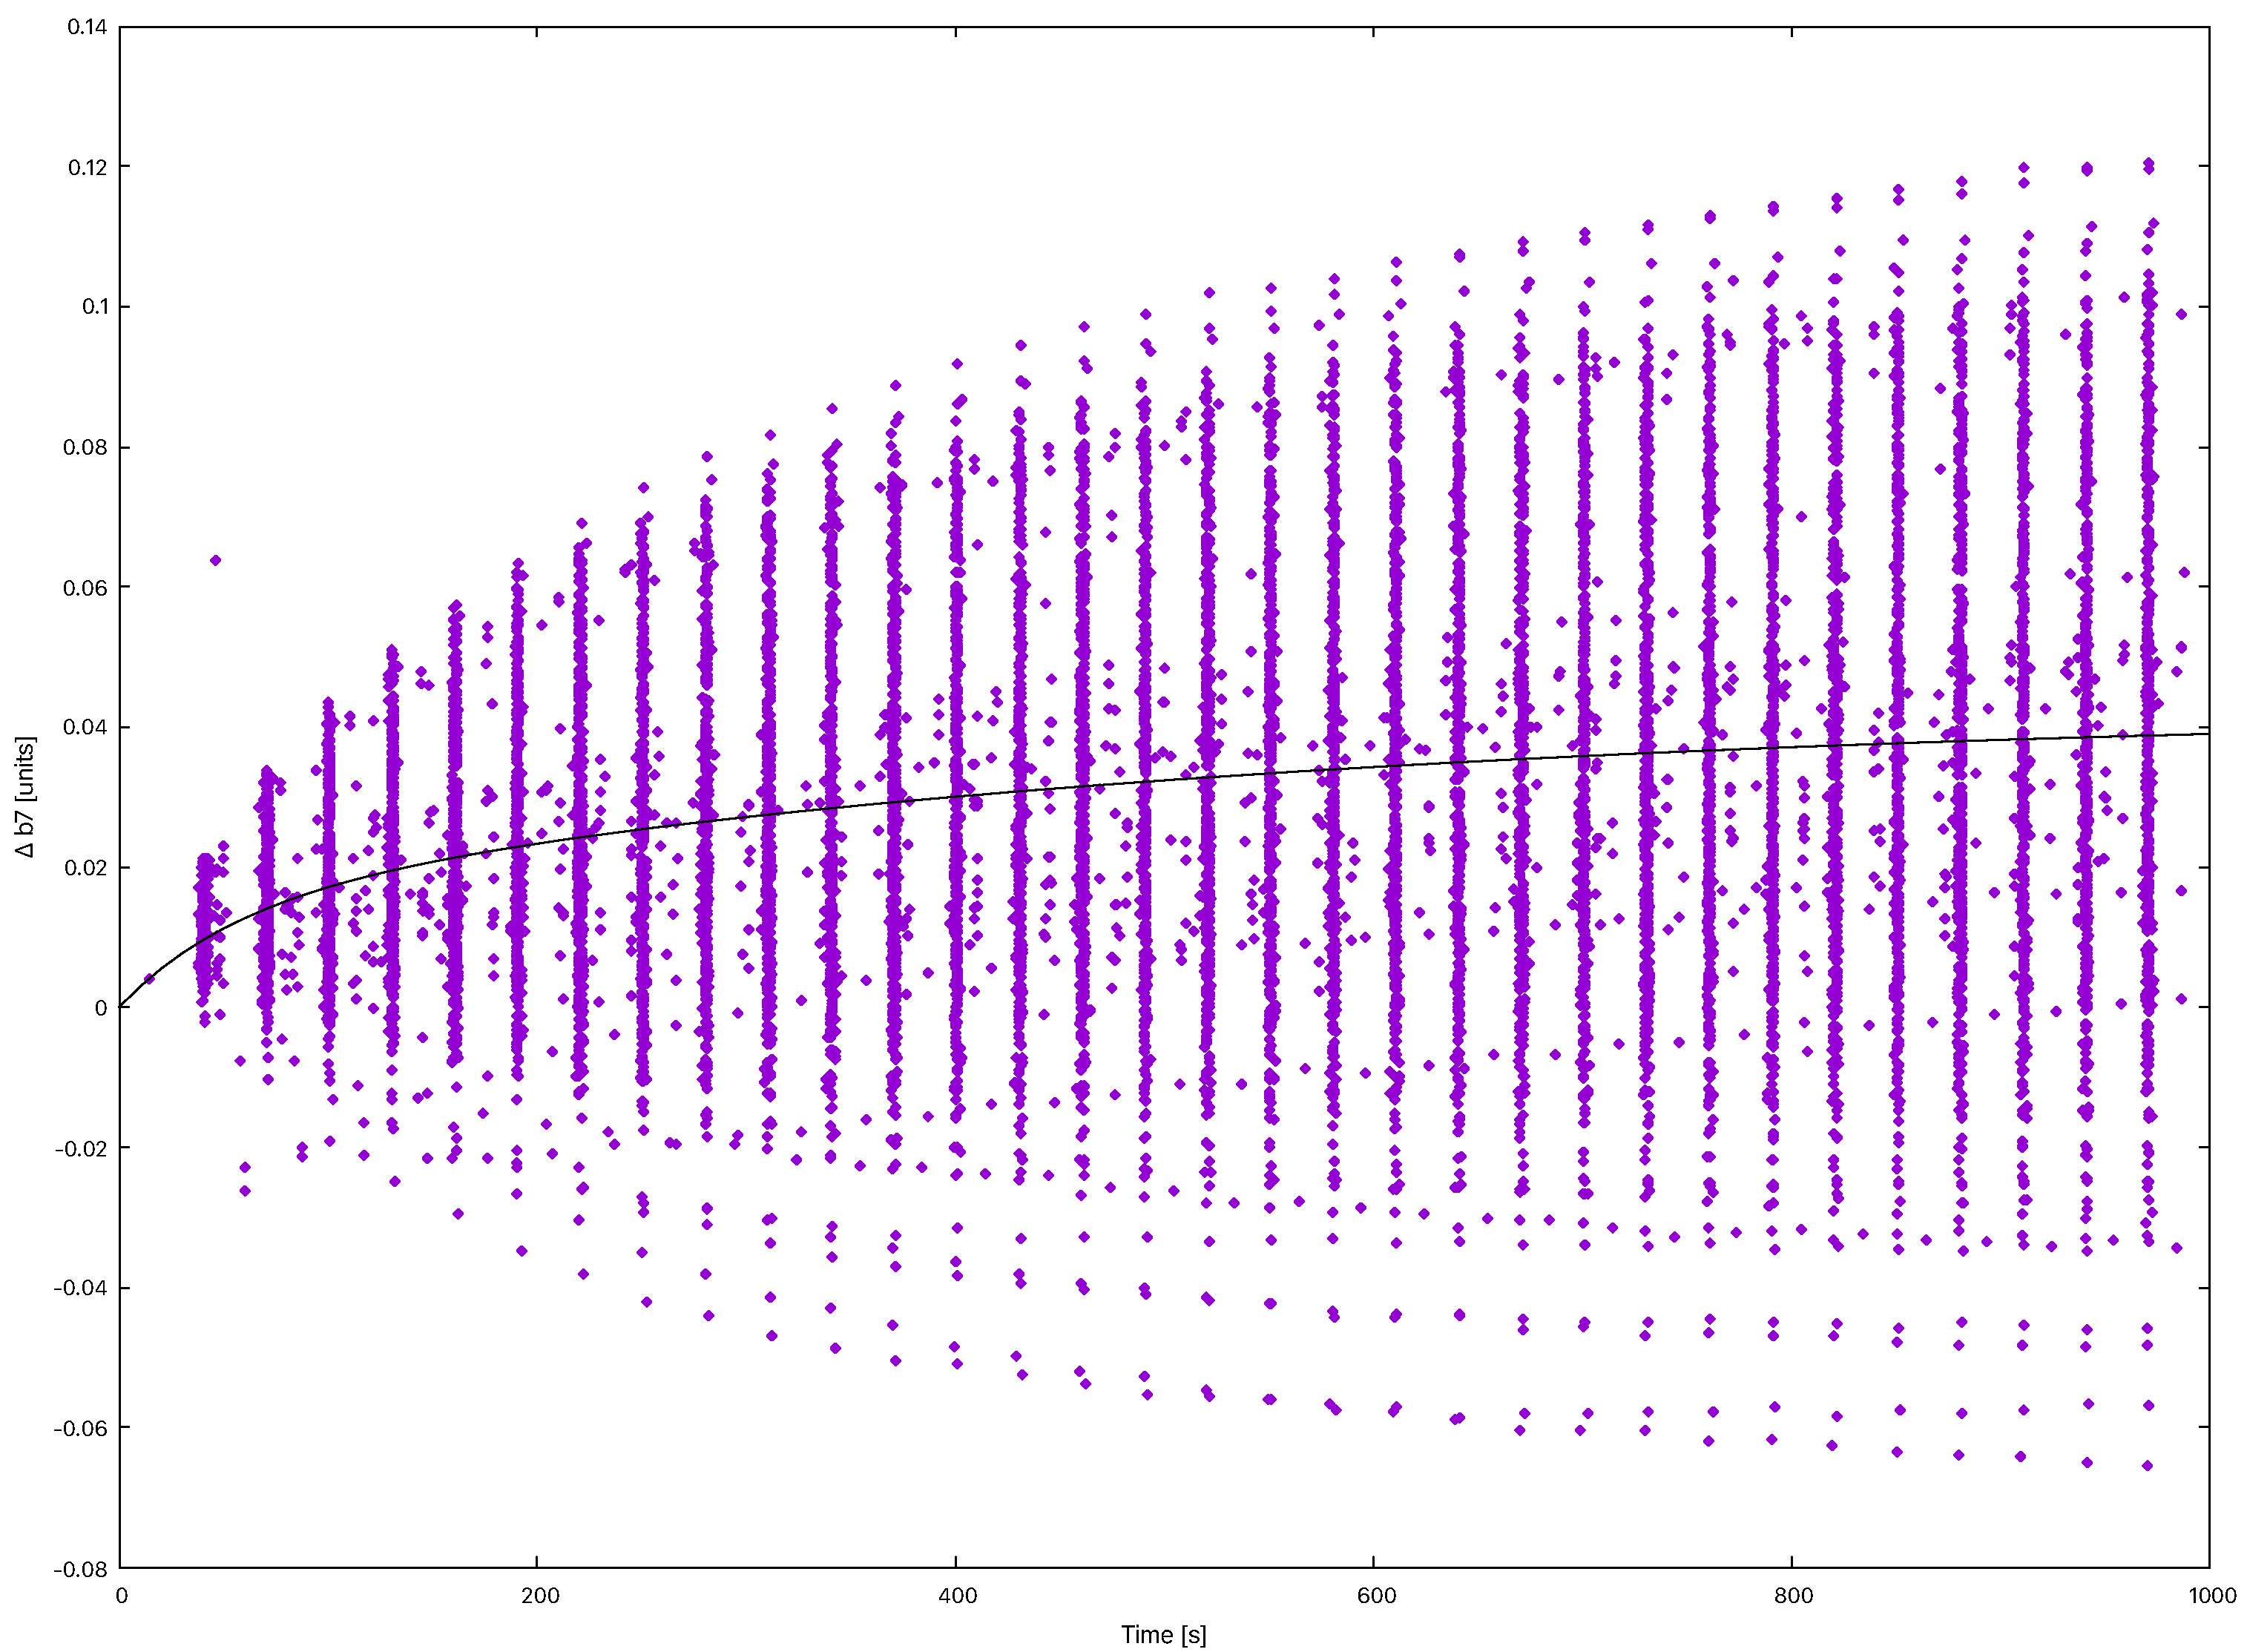
\includegraphics[width=0.9\columnwidth]{images/decay_b7.pdf}
    \caption{Measured decay of the integrated decatetrapolar field in LHC's main dipoles at
    injection energy. The fit is shown in black~\cite{deniau2024private} and settles around
    $+0.035$.}
    \label{fig:high_orders:b7_decay}
\end{figure}

Its value is though small and settles around $+0.0351 \pm 0.0007$. The average $b_7$ of the main
dipoles is of $0.32 \pm 0.16$. The decay thus increase that value of only about $11\%$.
Simulations done with that decay taken into account are detailed next.


% =================================
\subsection{\review{Major contributions}}

Simulations with various field errors have been run to assess the contribution of individual magnet
order and combinations for the fourth and firth order chromaticity. Normal and skew fields errors
ranging from sextupolar ($b_3$) to decahexapolar ($b_8$) are added alone or in combination to
observe which is the strongest. Quadrupolar field errors ($b_2$) introduce beta-beating. Coupling is
introduced via skew quadrupolar correctors.


% ----------------------------------
\subsubsection{\review{Fourth Order Chromaticity}}

The results from simulations strongly imply that the dodecapolar errors are the main contributors
to $Q^{(4)}$, as can be seen in \cref{fig:high_orders:beam1_q4_ptc}.
Fringe fields have a negligible impact, as do skew multipoles.
The most notable effect on this chromaticity order is the beta-beating, introducing a very large
spread via the various error seeds.
Comparing the simulation at the top with most errors added, the $b_6$ component alone accounts for
$\approx 70\%$ of it for both axes on each beam.

\begin{figure}[!htb]
    \centering
    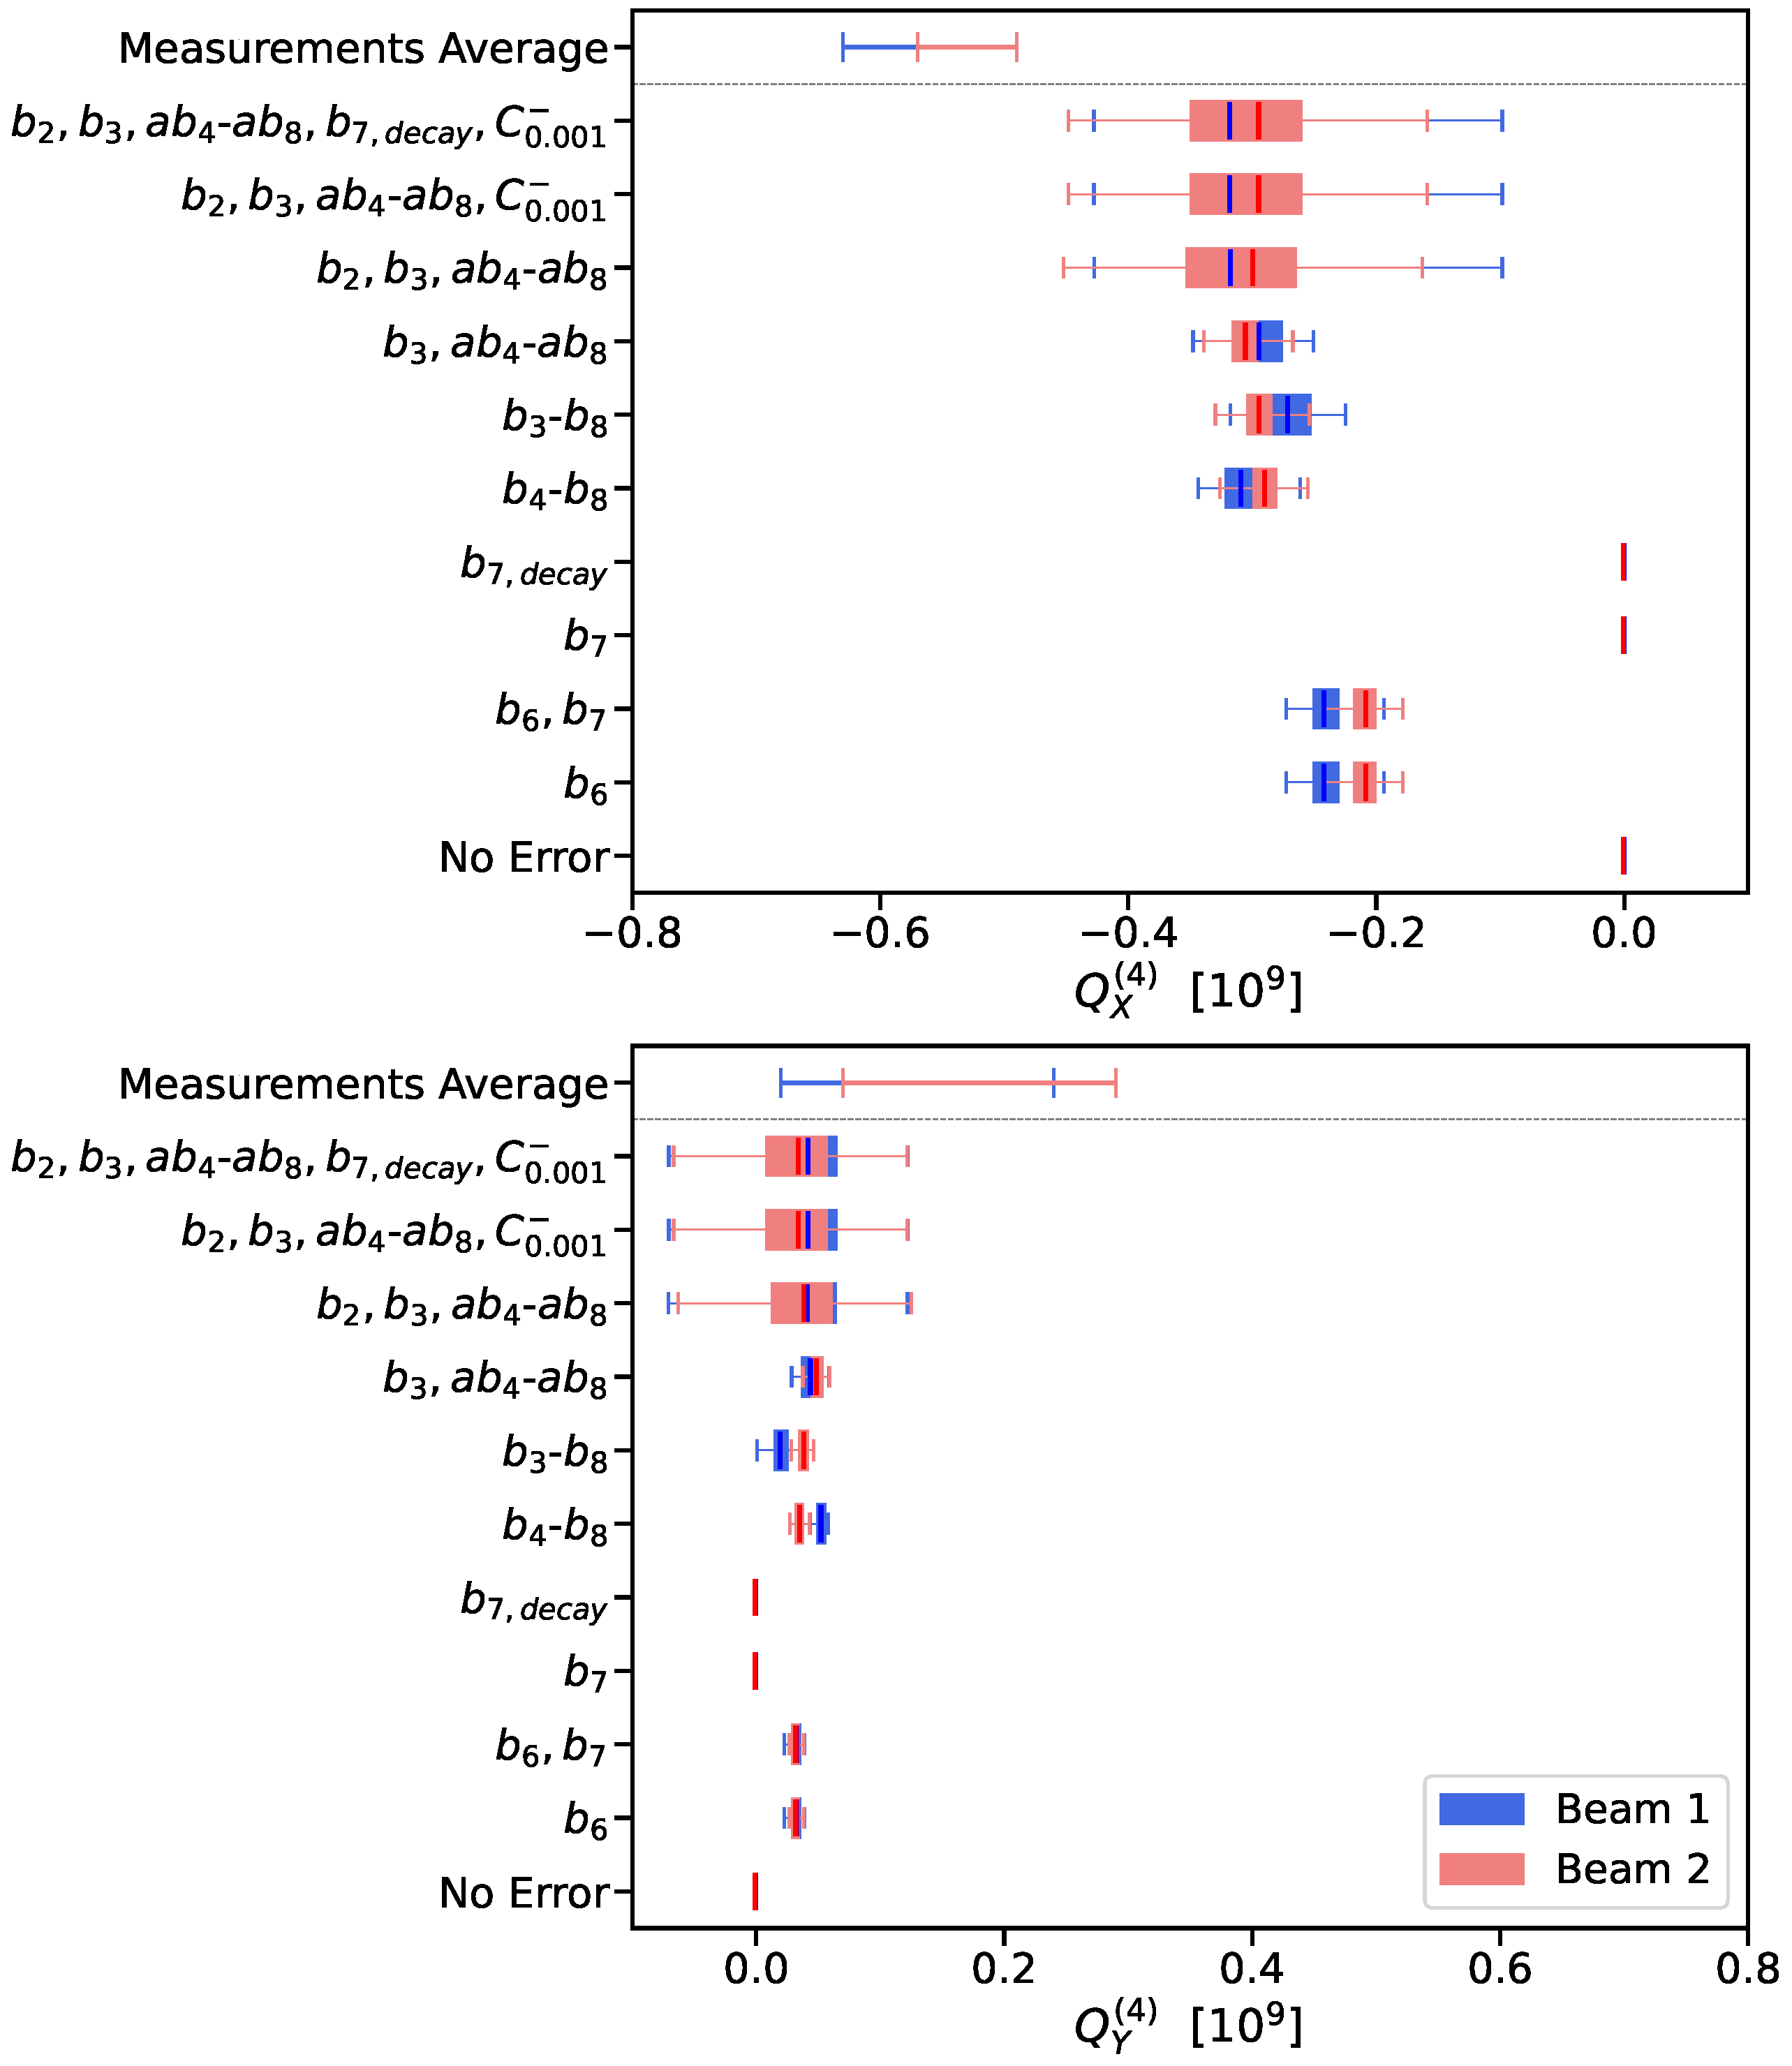
\includegraphics[width=0.9\columnwidth]{images/q4_ptc.pdf}
    \caption{Measured and simulated fourth order chromaticity with different multipole errors. The
    $b_2$ errors, applied on dipoles and quadrupoles, generate beta-beating. Coupling is set to a
    value commonly seen in operation.}
    \label{fig:high_orders:beam1_q4_ptc}
\end{figure}



% ----------------------------------
\subsubsection{\review{Fifth Order Chromaticity}}

It is seen that the the decatetrapolar errors are the main contributors to $Q^{(5)}$, as can be seen
in \cref{fig:high_orders:beam1_q5_ptc}. Fringe fields and skew multipoles have been found to have a
negligible impact. 
Beta-beating and coupling are seen to increase by a small amount the chromaticity, while sextupolar
errors induce a spread with the different seeds. 
As for the fourth order, comparing the simulation at the top with most errors added, the $b_7$
component alone accounts for $\approx 70\%$ of it for both axes on each beam of the fifth order
chromaticity.

\begin{figure}[!htb]
    \centering
    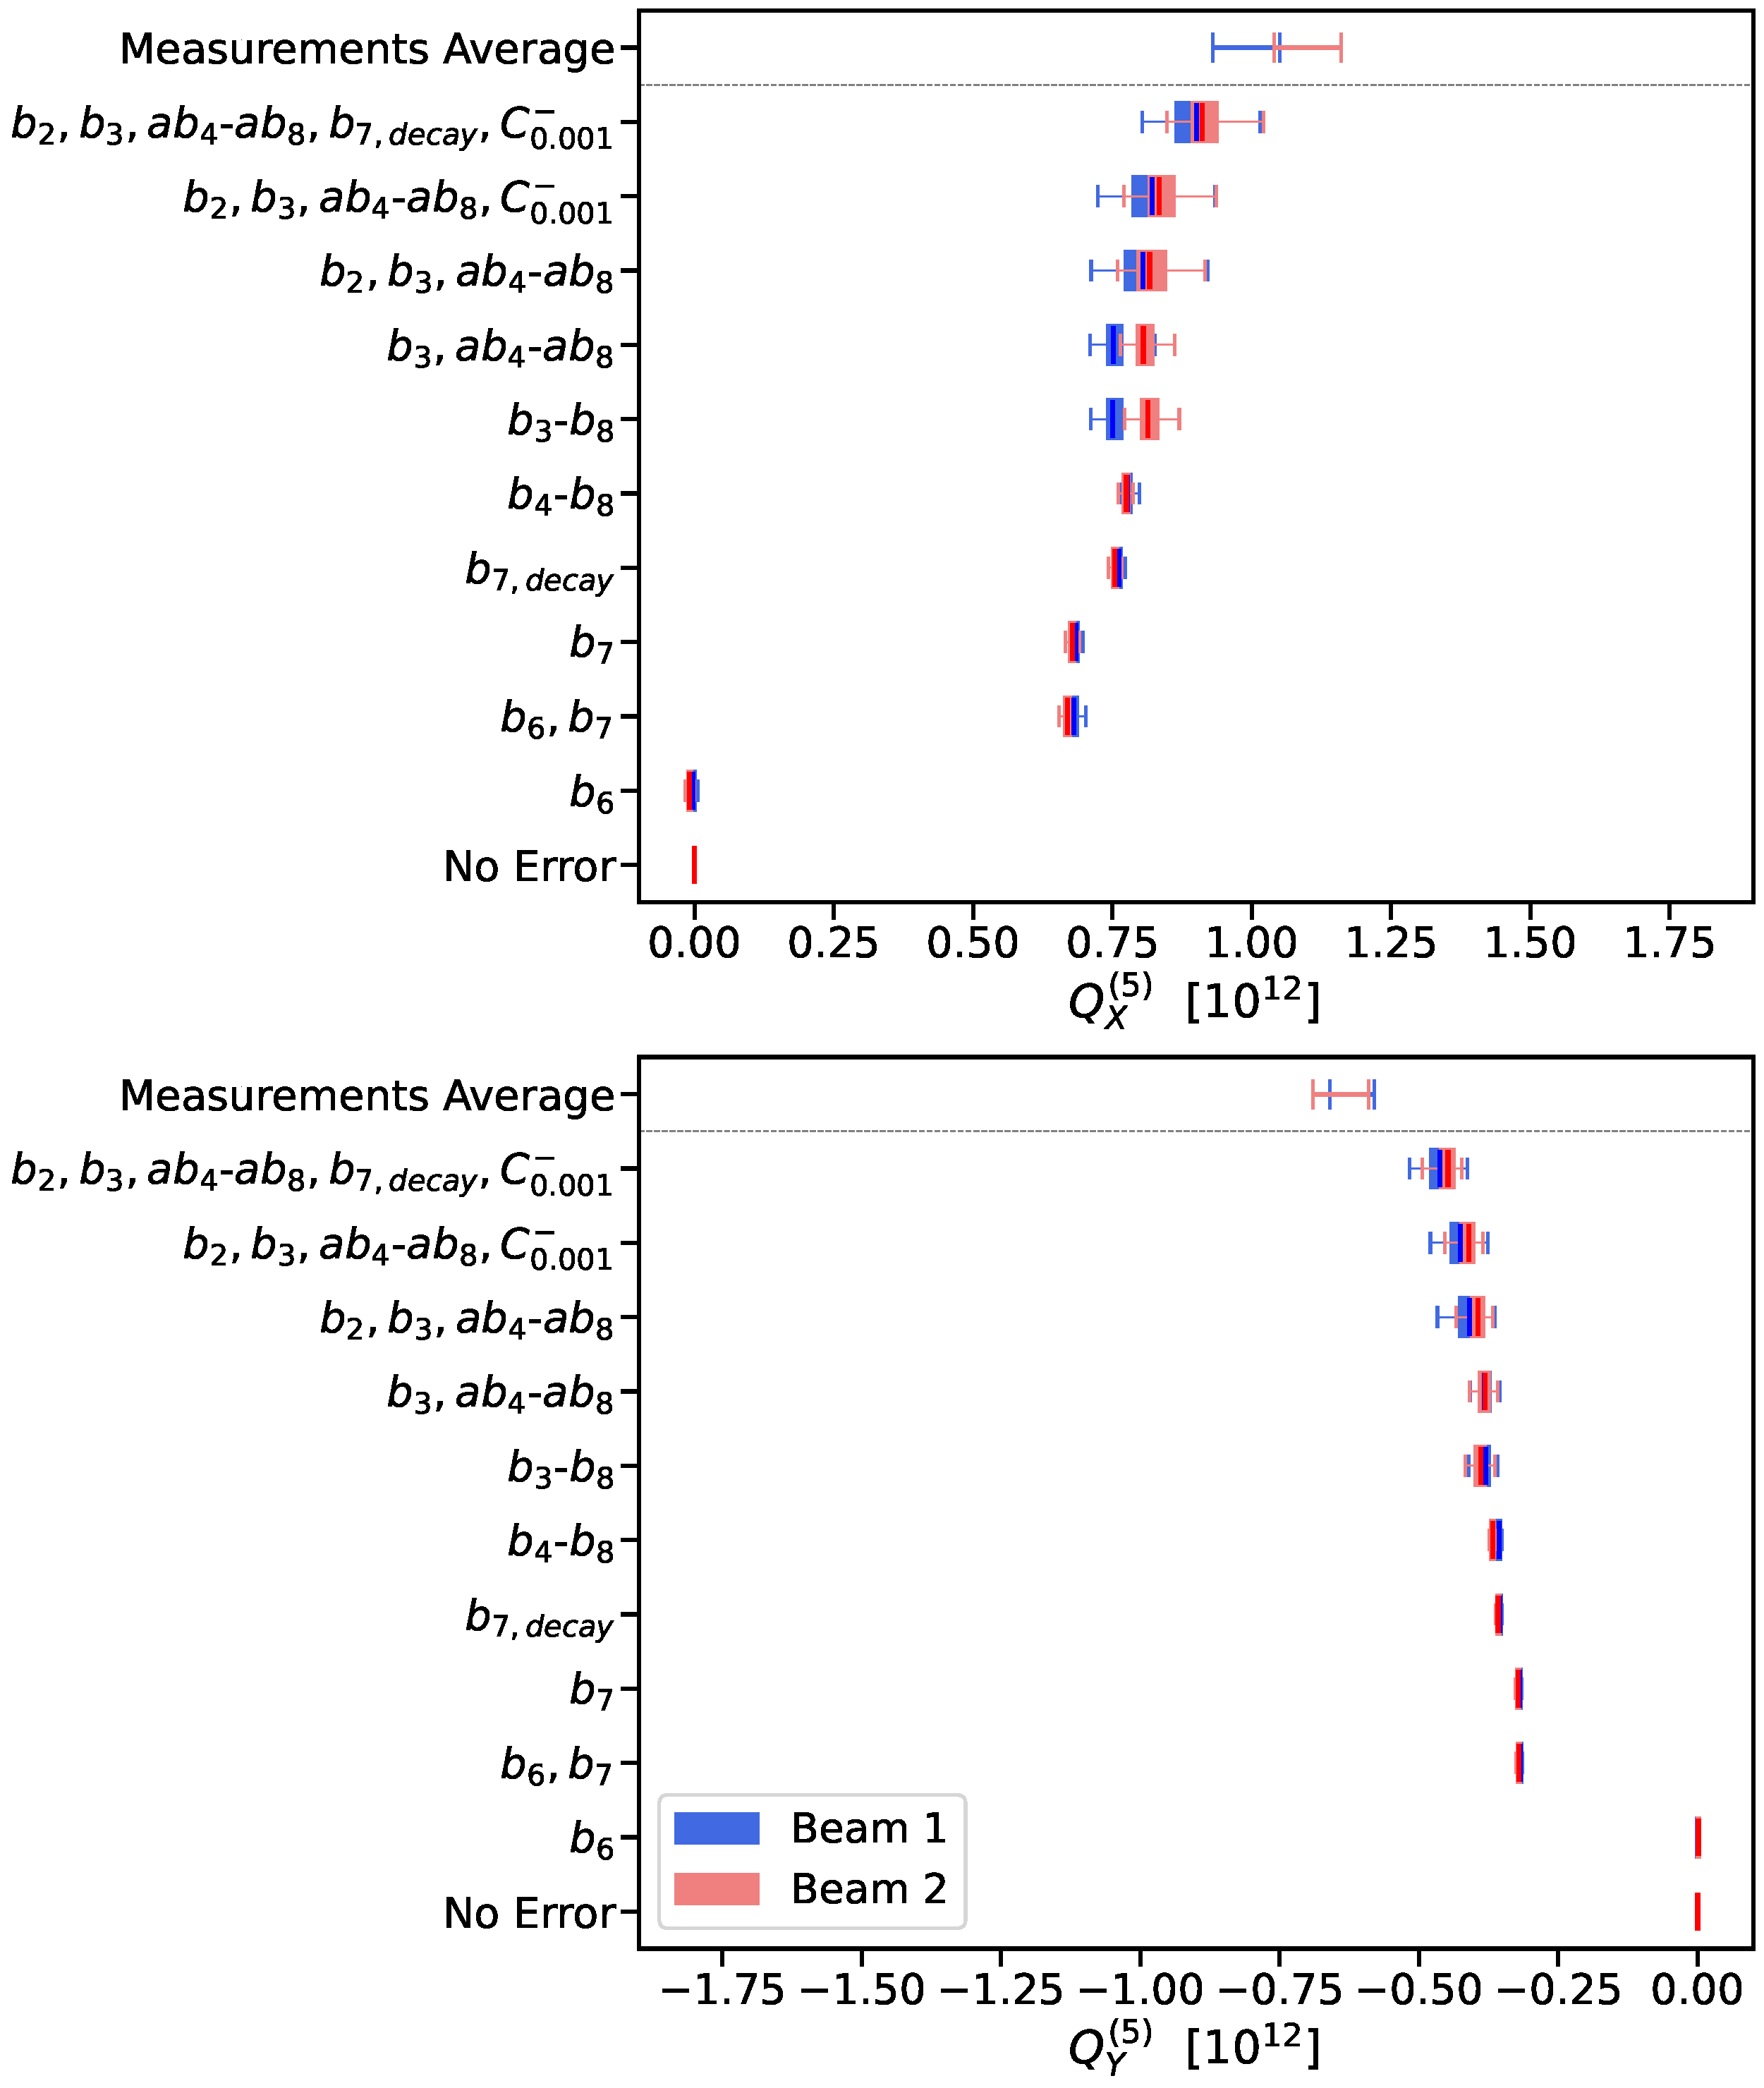
\includegraphics[width=0.9\columnwidth]{images/q5_ptc.pdf}
    \caption{Measured and simulated fifth order chromaticity with different multipole errors. The
    $b_2$ errors, applied on dipoles and quadrupoles, generate beta-beating. Coupling is set to a
    value commonly seen in operation.}
    \label{fig:high_orders:beam1_q5_ptc}
\end{figure}



% =================================
\subsection{\review{Ratios}}

Previous simulation results are shown in \cref{tab:high_orders:ptc_values}, taking the values from 
the simulation including the most effects at the top of the plots. For the fourth order, the beating
is not included as the large beating is not yet explained.
\Cref{tab:high_orders:ptc_values_ratios} shows the ratio between the measured average and simulated
chromaticities.

\begin{table}[!htb]
  \centering
  \begin{tabular}{lrr}
  \toprule
      Plane     &  $Q^{(4)} [10^9]$  &  $Q^{(5)} [10^{12}]$ \\
  \midrule
      Beam 1    &              &               \\
      \hspace{2mm}X         & $-0.29 \pm 0.02$ & $ 0.90 \pm 0.05$  \\
      \hspace{2mm}Y         & $ 0.04 \pm 0.01$ & $-0.46 \pm 0.03$  \\
      Beam 2    &  &   \\
      \hspace{2mm}X         & $-0.31 \pm 0.02$ & $ 0.92 \pm 0.03$ \\
      \hspace{2mm}Y         & $ 0.05 \pm 0.00$ & $-0.45 \pm 0.01$ \\
  \bottomrule
  \end{tabular}
  \caption{Simulated high order chromaticity terms via PTC at injection energy, including normal and
  skew sextupolar to decahexapolar field errors. Are also included beta-beating, coupling and
  decatetrapolar decay. For the fourth order, the values do not include beta-beating as the observed
  spread is not yet fully understood.}
  \label{tab:high_orders:ptc_values}
\end{table}

%\begin{table}[!htb]
%  \centering
%  \footnotesize
%  \begin{tabular}{lcccc}
%    \toprule
%                    &  \multicolumn{2}{c}{$Q^{(4)}$ Ratio}   &  \multicolumn{2}{c}{$Q^{(5)}$ Ratio} \\
%    \cmidrule(lr){2-3}\cmidrule(lr){4-5}
%      Plane         & First Meas.  & Second Meas.& First Meas.& Second Meas. \\ 
%    \midrule
%      Beam 1        &           &             &            & \\
%      \hspace{2mm}X &  $1.91\pm0.15$ & $2.15\pm0.17$    & $1.33\pm0.10$  & $1.35\pm0.09$   \\
%      \hspace{2mm}Y &  $3.50\pm0.90$ & $0.90\pm0.50$    & $1.91\pm0.22$  & $1.21\pm0.11$   \\
%      Beam 2        &                   &               &     & \\
%      \hspace{2mm}X &                & $4.90\pm1.00$    &                & $1.17\pm0.08$   \\
%      \hspace{2mm}Y &  $1.90\pm0.12$ & $3.30\pm0.50$    & $1.65\pm0.29$  & $1.47\pm0.12$   \\
%      \bottomrule
%  \end{tabular}
%  \caption{Ratios of the simulated and measured high order chromaticity terms for both the first and
%  second performed measurements. The values are taken from tables
%  \cref{tab:high_orders:chroma_fidel}, \cref{tab:high_orders:chroma_table_after} and
%  \cref{tab:high_orders:ptc_values}. The fit with high correlation between both terms is not
%  included.}
%  \label{tab:high_orders:ptc_values_ratios}
%\end{table}

\begin{table}[!htb]
    \centering
    \begin{tabular}{lcc}
      \toprule
        Plane         & $Q^{(4)}$ Ratio&  $Q^{(5)}$ Ratio \\
      \midrule
        Beam 1        &                &                  \\
        % Via weighted mean, which is probably not right.
        %\hspace{2mm}X &  $1.98\pm0.16$ & $1.10\pm0.09$    \\
        %\hspace{2mm}Y &  $3.00\pm0.70$ & $1.34\pm0.11$    \\
        \hspace{2mm}X &  $1.91\pm0.28$ & $1.24\pm0.23$    \\
        \hspace{2mm}Y &  $3.00\pm2.60$ & $1.47\pm0.27$    \\
        Beam 2        &                &                  \\
        %\hspace{2mm}X &  $1.74\pm0.11$ & $1.20\pm0.08$    \\
        %\hspace{2mm}Y &  $2.90\pm0.50$ & $1.42\pm0.12$    \\
        \hspace{2mm}X &  $1.74\pm0.16$ & $1.34\pm0.29$    \\
        \hspace{2mm}Y &  $3.70\pm2.30$ & $1.51\pm0.14$    \\
        \bottomrule
    \end{tabular}
    \caption{Ratios of the simulated and average measured high-order chromaticity terms.  The values
    are taken from \cref{fig:high_oders:all_values} and \cref{tab:high_orders:ptc_values}.}
    \label{tab:high_orders:ptc_values_ratios}
\end{table}

The similar ratios between planes and beams for the fifth order could indicate a systematic error
not modeled.
The large differences observed for the fourth order are not yet explained but the difference between
planes could be linked to a shift induced by the decapolar corrections in the vertical plane. It
indeed seems that the fourth order follows a trend with the third order.
\todo{check correlation between Q3 Q4}


%=============================
%            RDTs
%=============================
\section{\todo{Dodecapolar RDTs}}

\begin{figure}[!htb]
    \centering
    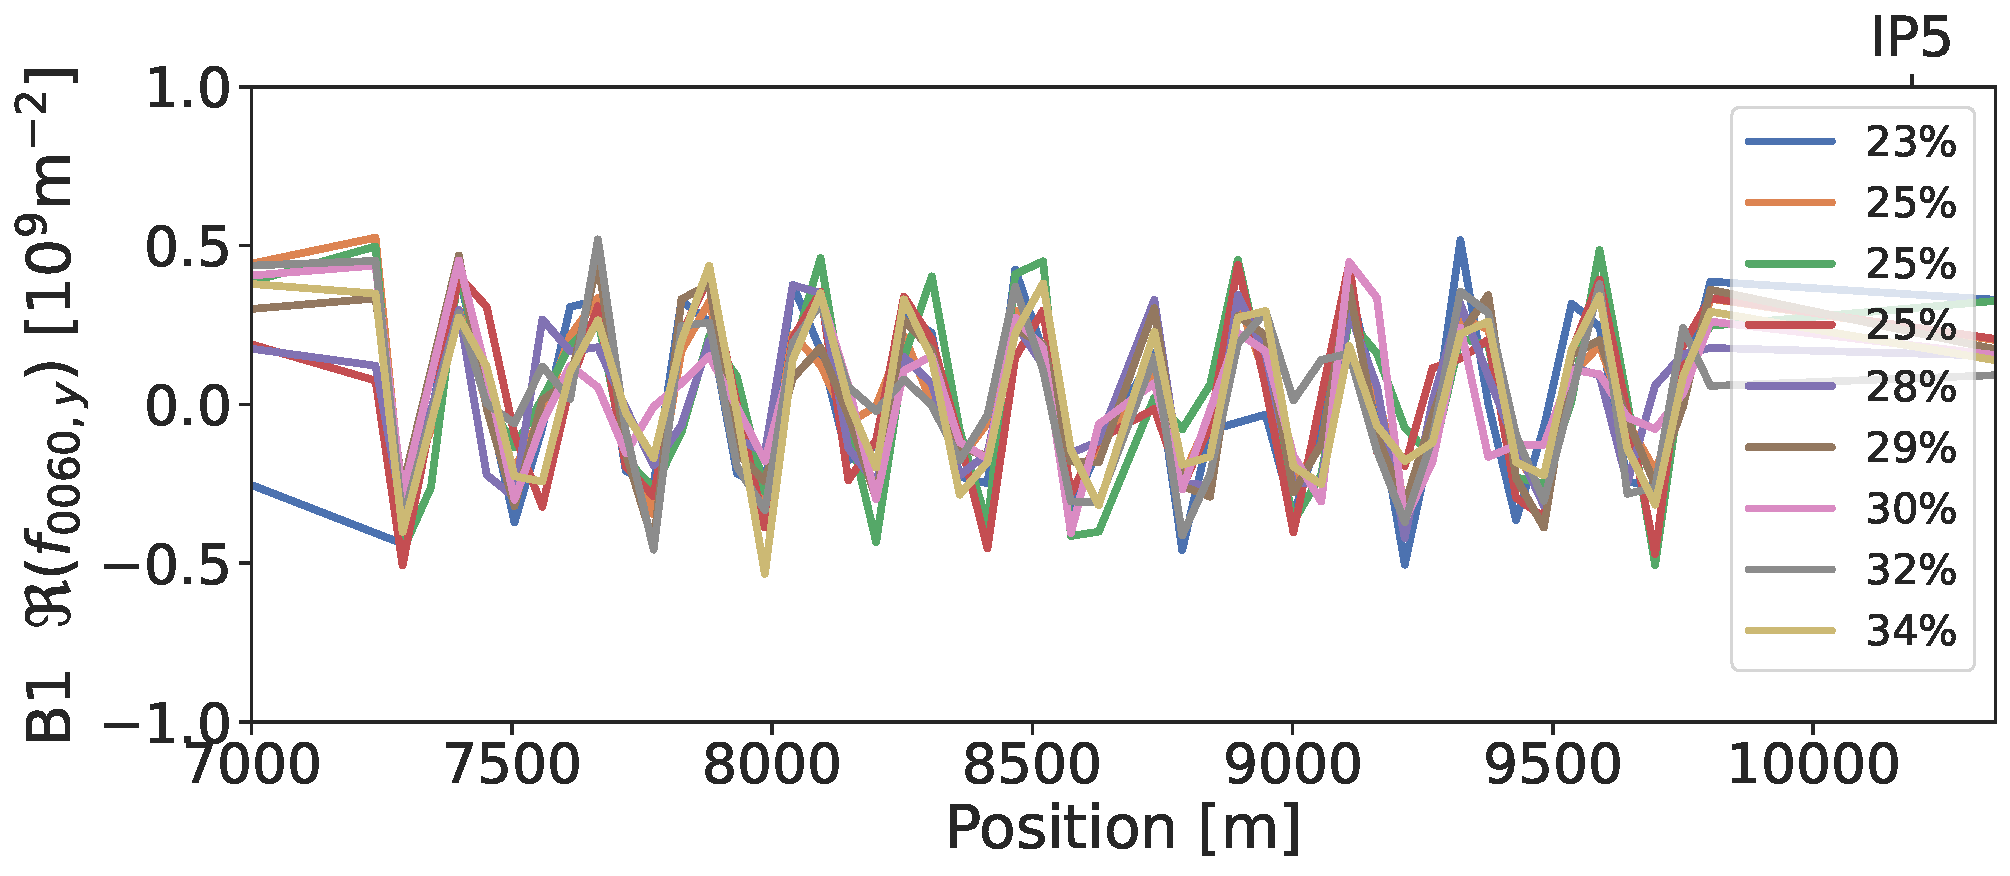
\includegraphics[width=\textwidth]{./images/f0060y_all_meas_real.pdf}
    \caption{Real part of the dodecapolar RDT $f_{0060}$ measured with several kick strengths. The
    RMS amplitude is of $0.35\cdot10^{9}$.}
    \label{fig:high_orders:chroma_nominal_correction_full_range}
\end{figure}





%=============================
%          Further
%=============================
\section{\todo{Going Further}}

% --------------------------------
%          Chromaticity
% --------------------------------
\subsection{\review{Chromaticity}}

% --------------------------------
%          High Ranges
\subsubsection{\review{Limitations}}

So far, the momentum offset ranges of the 2024 measurements have been restricted in order to allow a 
comparison with the shorter ranges measurements made in 2022. The non-linearity of the chromaticity 
and its higher orders become very noticeable once these large ranges are reached.
\Cref{fig:high_orders:chroma_nominal_correction_full_range} shows an example of such measurement for 
Beam 2, made with the nominal corrections, highlighting the difference between two momentum offset
ranges.

\begin{figure}[!htb]
    \begin{subfigure}{0.49\textwidth}
        \centering
        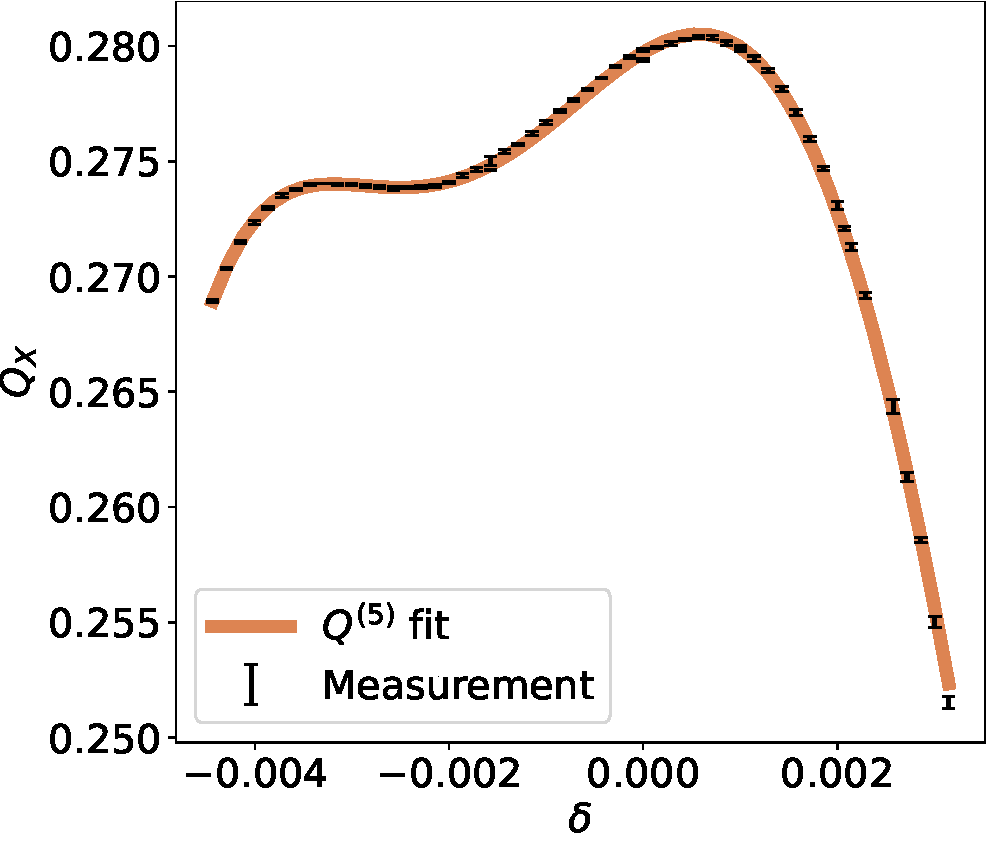
\includegraphics[width=\textwidth]{./images/chromaticity_further/q5_range/Beam2_Qx_full_but_not_quite.pdf}
        \caption{$Q_x$ Beam 2 High Range}
    \end{subfigure}
    \hfill
    \begin{subfigure}{0.49\textwidth}
        \centering
        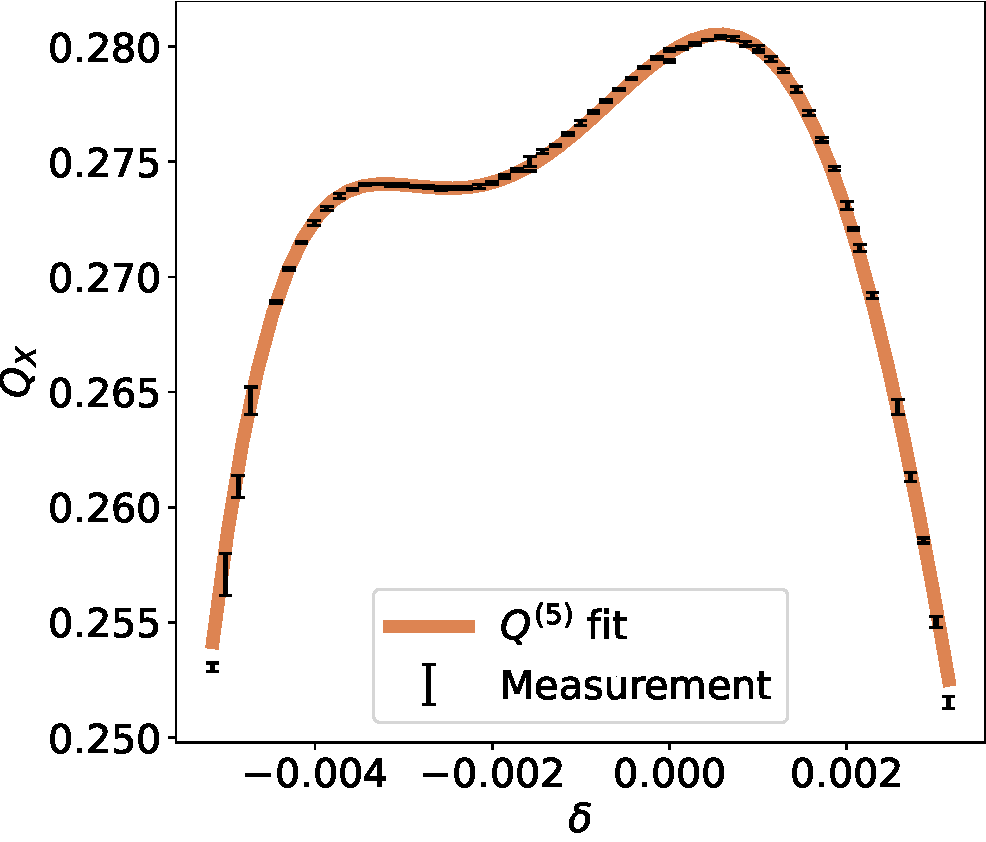
\includegraphics[width=\textwidth]{./images/chromaticity_further/q5_range/Beam2_Qx_full.pdf}
        \caption{$Q_y$ Beam 2 Full Range}
    \end{subfigure}
    %
    \caption{Third Beam 2 measurement of \cref{table:high_orders:dpp_ranges} with nominal
    corrections. A very large momentum offset range clearly highlights the non-linearity of the
    chromaticity function.}
    \label{fig:high_orders:chroma_nominal_correction_full_range}
\end{figure}

\begin{table}[!htb]
    \centering
    \begin{tabular}{lcccc}
      \toprule
      Plane & $Q^{(2)} [\times 10^{3}]$ & $Q^{(3)} [\times 10^{6}]$ & $Q^{(4)} [\times 10^{9}]$ & $Q^{(5)} [\times 10^{12}]$ \\
      \midrule
      X &&&& \\  
      \hspace{2mm}Rest. Range &$-2.93 \pm 0.05$ & $-4.40 \pm 0.08$ & $-0.53 \pm 0.08$ & $ 1.66 \pm 0.16$ \\
      \hspace{2mm}High Range  &$-2.99 \pm 0.05$ & $-4.71 \pm 0.03$ & $-0.42 \pm 0.07$ & $ 2.23 \pm 0.07$ \\
      \hspace{2mm}Full Range  &$-3.05 \pm 0.05$ & $-4.75 \pm 0.03$ & $-0.33 \pm 0.07$ & $ 2.34 \pm 0.06$ \\
      Y &&&& \\  
      \hspace{2mm}Rest. Range &$ 0.89 \pm 0.02$ & $ 2.05 \pm 0.03$ & $ 0.32 \pm 0.03$ & $-0.73 \pm 0.06$ \\
      \hspace{2mm}High Range  &$ 0.87 \pm 0.02$ & $ 2.07 \pm 0.02$ & $ 0.36 \pm 0.03$ & $-0.77 \pm 0.03$ \\
      \hspace{2mm}Full Range  &$ 0.70 \pm 0.04$ & $ 1.83 \pm 0.03$ & $ 0.64 \pm 0.06$ & $-0.32 \pm 0.05$ \\
      \bottomrule
    \end{tabular}
    \caption{Variance of the chromaticity values depending on the considered momentum offset range.
    All ranges have an upper bound of $3.2\times10^{-3}$. The lower bounds are, in order of
    appearance: $-3.5$, $-4.5$, $-5.2$.}
    \label{tab:high_orders:further:chroma_different_ranges}
  \end{table}

\Cref{tab:high_orders:further:chroma_different_ranges} shows the obtained chromaticity values for
varying ranges. From this table, it can be noted that increasing the range mainly
changes the estimate for $Q^{(5)}_x$.
Measurements over such a wide range are not yet fully understood, as other non-linear effects can
induce a detuning. For example, transverse impedances leads to a defocusing effect whose magnitude
increases with the orbit offset~\cite{antipov_single-collimator_2018,kurtulus_lhc_2022}.
Some other performed measurements with wide ranges in 2024 could not be fitted with a chromaticity
function, despite including higher orders. It is deemed that restricting the ranges is beneficial to
the fit estimates, until further investigation of these effects.



% --------------------------------
%       Even Higher Orders?
\subsubsection{\review{Higher Orders}}

The fifth measurement in \cref{table:high_orders:dpp_ranges} covered a range of $[-4.0 \cdot
10^{-3}, 4.5 \cdot 10^{-3}]$, which is among the widest ever measured. It is clear from
\cref{fig:high_orders:chroma_after_correction_full_range} that a chromaticity function including the
sixth order provides a better fit to the data. However, no additional observations were made for
this order, and considering the previously mentioned limitations, this measurement may not be
entirely robust. Further studies could address these limitations to more accurately characterize the
decahexapolar fields of the LHC at injection energy.

\begin{figure}[!htb]
    \begin{subfigure}{0.49\textwidth}
        \centering
        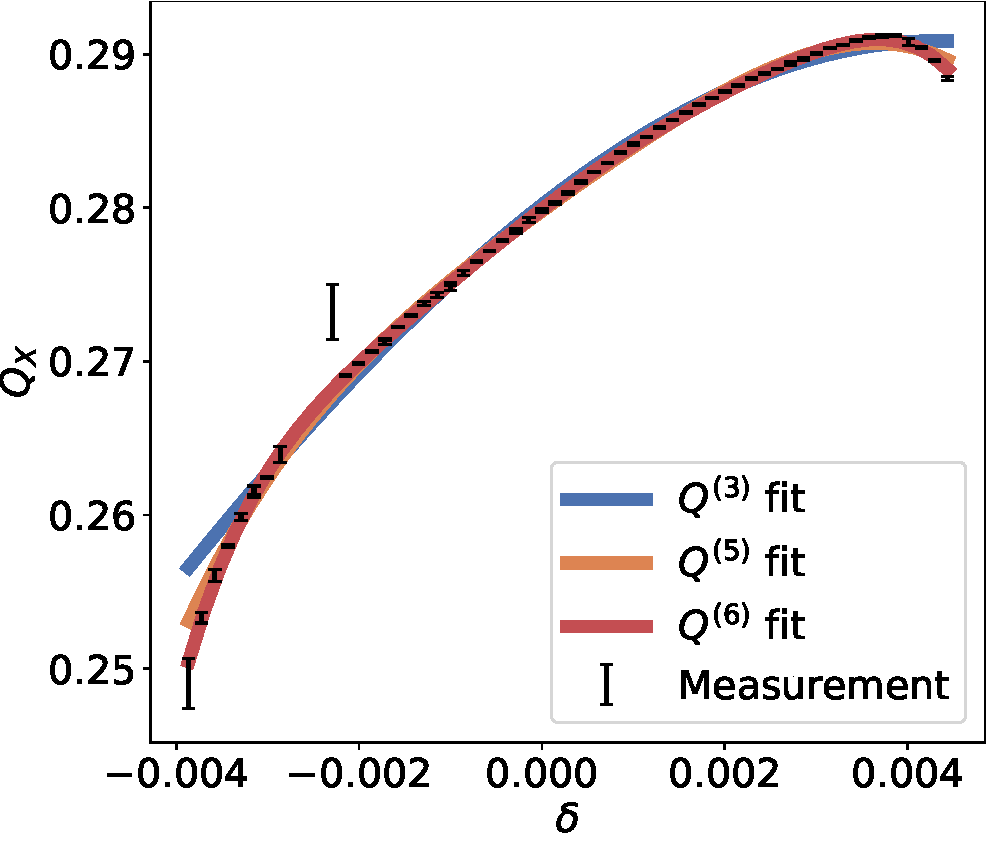
\includegraphics[width=\textwidth]{./images/chromaticity_further/q6/Beam1_Qx.pdf}
        \caption{$Q_x$ Beam 1}
    \end{subfigure}
    \hfill
    \begin{subfigure}{0.49\textwidth}
        \centering
        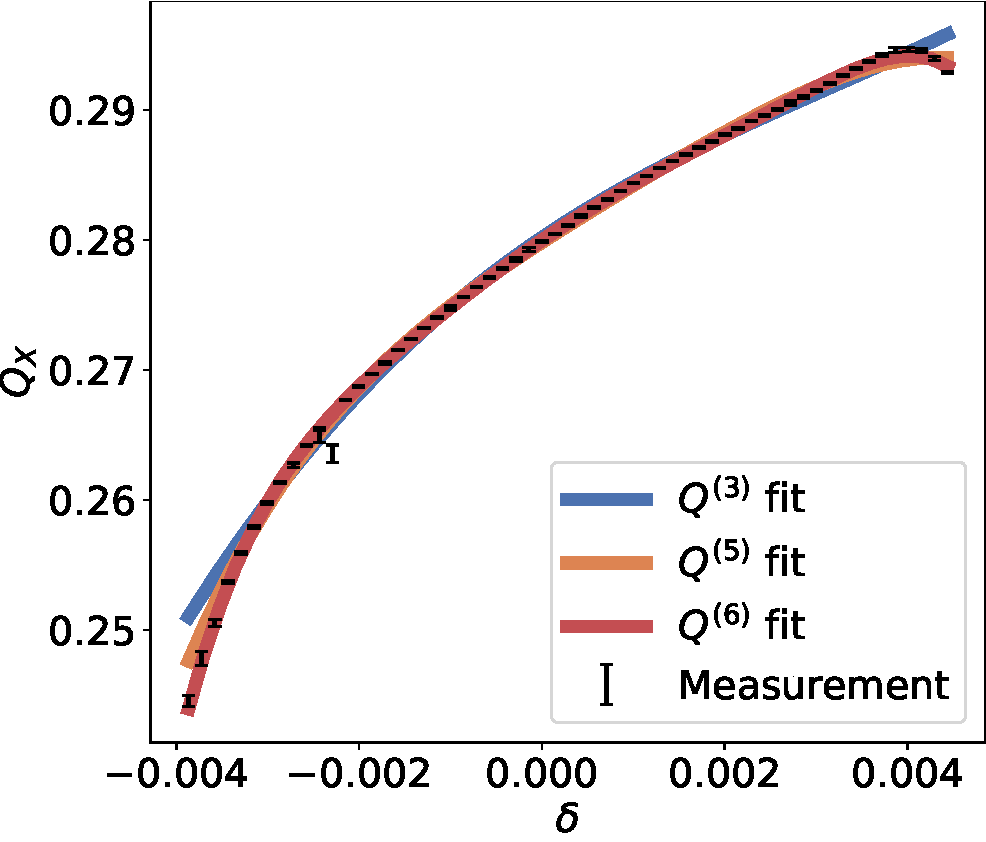
\includegraphics[width=\textwidth]{./images/chromaticity_further/q6/Beam2_Qx.pdf}
        \caption{$Q_x$ Beam 2}
    \end{subfigure}
    %
    \caption{Fifth measurement of \cref{table:high_orders:dpp_ranges} with $Q''$ and $Q'''$
    corrections. A possible sixth chromaticity order can be seen.}
    \label{fig:high_orders:chroma_after_correction_full_range}
\end{figure}




% --------------------------------
%          RDT
% --------------------------------
\subsection{\todo{Resonance Driving Terms}}

corrections? relevance? DA? 


%=============================
%        Conclusion
%=============================
\section{\todo{Summary}}

A wider momentum offset range, combined with new analysis techniques permitted the observation of
the fourth and fifth order of the chromaticity function for the first time in the LHC. Reproducible
values were measured with different machine configurations.

Simulations show that the observed values do not match well with the LHC non-linear model. A factor
$\approx 1.5$ is observed between measurements and simulations for $Q^{(5)}$, which may point to a
systematic error in the b7 error model.

Correction of the measured higher order chromaticity terms is not possible, due to the lack of
adequate correctors in the LHC. It is nevertheless interesting to characterize the higher order
errors for an effective model and understand the effect a higher order fit has on lower order terms.
Precise measurement of those lower chromaticity terms is required in order to effectively correct
them. Higher order terms have thus to be taken into account.

The current range of momentum offset is deemed sufficient to measure higher order chromaticity.
Attempts will, however, be taken to increase that range and assess if such a wider range can refine
the estimate of $Q^{(4)}$ and $Q^{(5)}$.
%=============================
%        Introduction
%=============================
\section{\review{Introduction}}

The skew octupolar fields in the LHC have previously been identified as significant contributors to 
limits in forced dynamic aperture, being the dynamic aperture when kicking the beam with the
AC-Dipole~\cite{carlier_nonlinear_2020}. Skew octupolar correctors are positioned around the
ATLAS and CMS detectors, in Interaction Regions 1 and 5. Those correctors are \textit{common
aperture} magnets ; both beams are affected by the created magnetic fields. Unfortunately, one of
these four correctors, located to the left of ATLAS, is not functioning. As a result, although
corrections can be calculated, they will not effectively minimize the skew octupolar RDTs of
interest, $f_{1012,y}$ and $f_{1210,x}$. 
The associated resonances and frequency lines of these RDTs are shown in
\cref{tab:skew_octupolar:resonances_rdts}.

\begin{table}[!htb]
    \centering
    \begin{tabular}{lccc}
      \toprule
      RDT         & Resonance                &  H-line                    & V-line         \\
      \midrule
      $f_{1012}$  & $\phantom{-}1Q_x - 1Q_y$ &  $\phantom{2Q_x-\ \,}1Q_y$ & $-1Q_x + 2Q_y$ \\
      $f_{1210}$  & $-1Q_x + 1Q_y$           &  $2Q_x - 1Q_y$             & $\phantom{-}1Q_x\phantom{+2Q_y\ \,}$    \\
      \bottomrule
    \end{tabular}
    \caption{Skew octupolar RDTs of interest, their associated resonances and the frequency spectrum
    lines they contribute to.}
    \label{tab:skew_octupolar:resonances_rdts}
\end{table}

First corrections of skew octupolar RDTs were performed in 2018 at top
energy~\cite{carlier_nonlinear_2020}. A different approach for the same corrections is presented in
this chapter.
Measurements were also performed at injection energy with the prospect of corrections. However, it
was observed that Landau octupoles were strongly contributing to the RDTs of interest.


%=============================
%         Top Energy
%=============================
\section{\review{Corrections at Top Energy}}

The very first skew octupolar RDT corrections in the LHC were made in 2018 during
Run~2~\cite{carlier_nonlinear_2020}. These corrections were computed by matching the RDT level of
the measurements in simulation and then inverting the strengths. This is possible and remains viable
as only three correctors are used and values can be manually adjusted.
In this section, a different approach is taken, based on response matrices. This type of correction
is explained in details in \cref{correction_principle:response_matrix}. The real and imaginary 
responses of the RDTs for each corrector at an arbitrary strength are simulated through tracking.
These responses are collected into a matrix, allowing the determination of the required strengths to
match the RDT level observed in the measurements. Inverting these values result in a correction.


%-----------------------------
%     Correctors Response
%-----------------------------
\subsection{\review{Correctors}}

To create a response matrix, simulations were conducted with the tunes and AC-Dipole deltas set to
those used for measurements. The natural tunes are $Q_x = 0.285$ and $Q_y = 0.292$ while the driven
tunes are $\Delta Q_x = -0.008$ and $\Delta Q_y = 0.01$. Each corrector is then powered
individually for each tracking simulation. For this type of simulation, field errors are not
necessary, as only the RDT shift caused by the corrector relative to the baseline is needed.
\Cref{fig:skew_octupolar:response_correctors} shows the real part of the resulting RDTs from these
simulations for Beam 1. Beam 2 shows a similar level of response for these correctors.

\begin{figure}[!htb]
    \centering
    \begin{subfigure}{0.8\textwidth}
        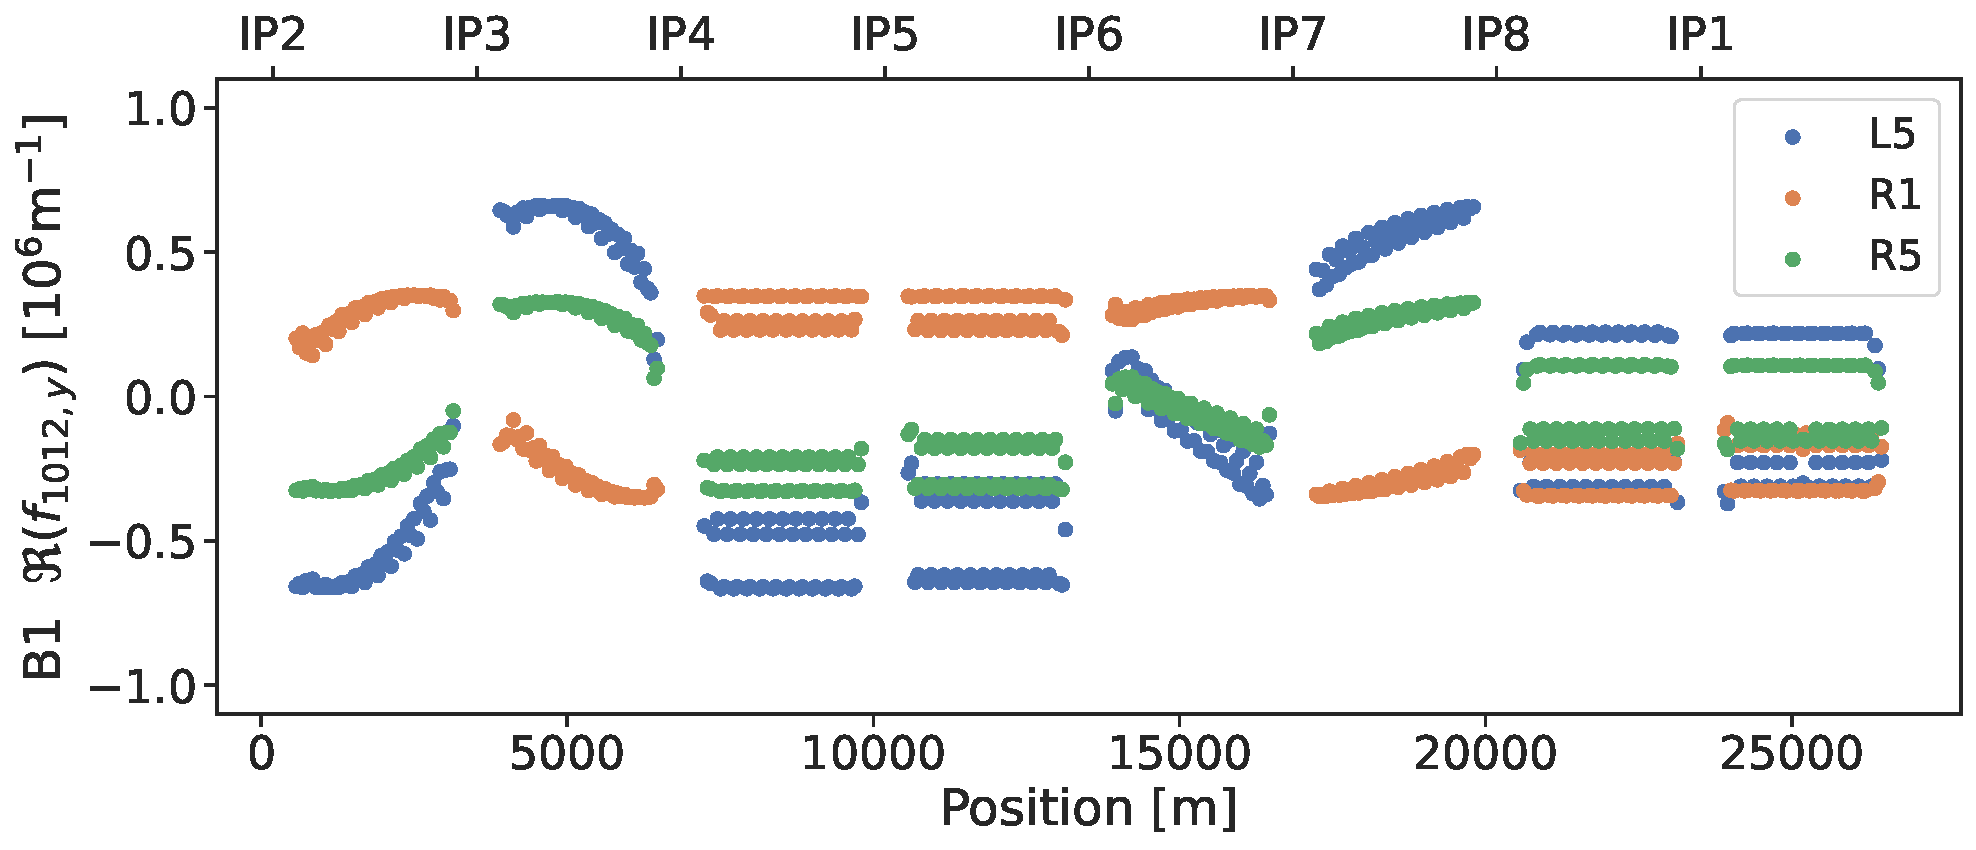
\includegraphics[width=\textwidth]{./images/f1012_b1_correctors.pdf}
        \caption{$f_{1012,y}$}
    \end{subfigure}
    \par\bigskip 
    \begin{subfigure}{0.8\textwidth}
        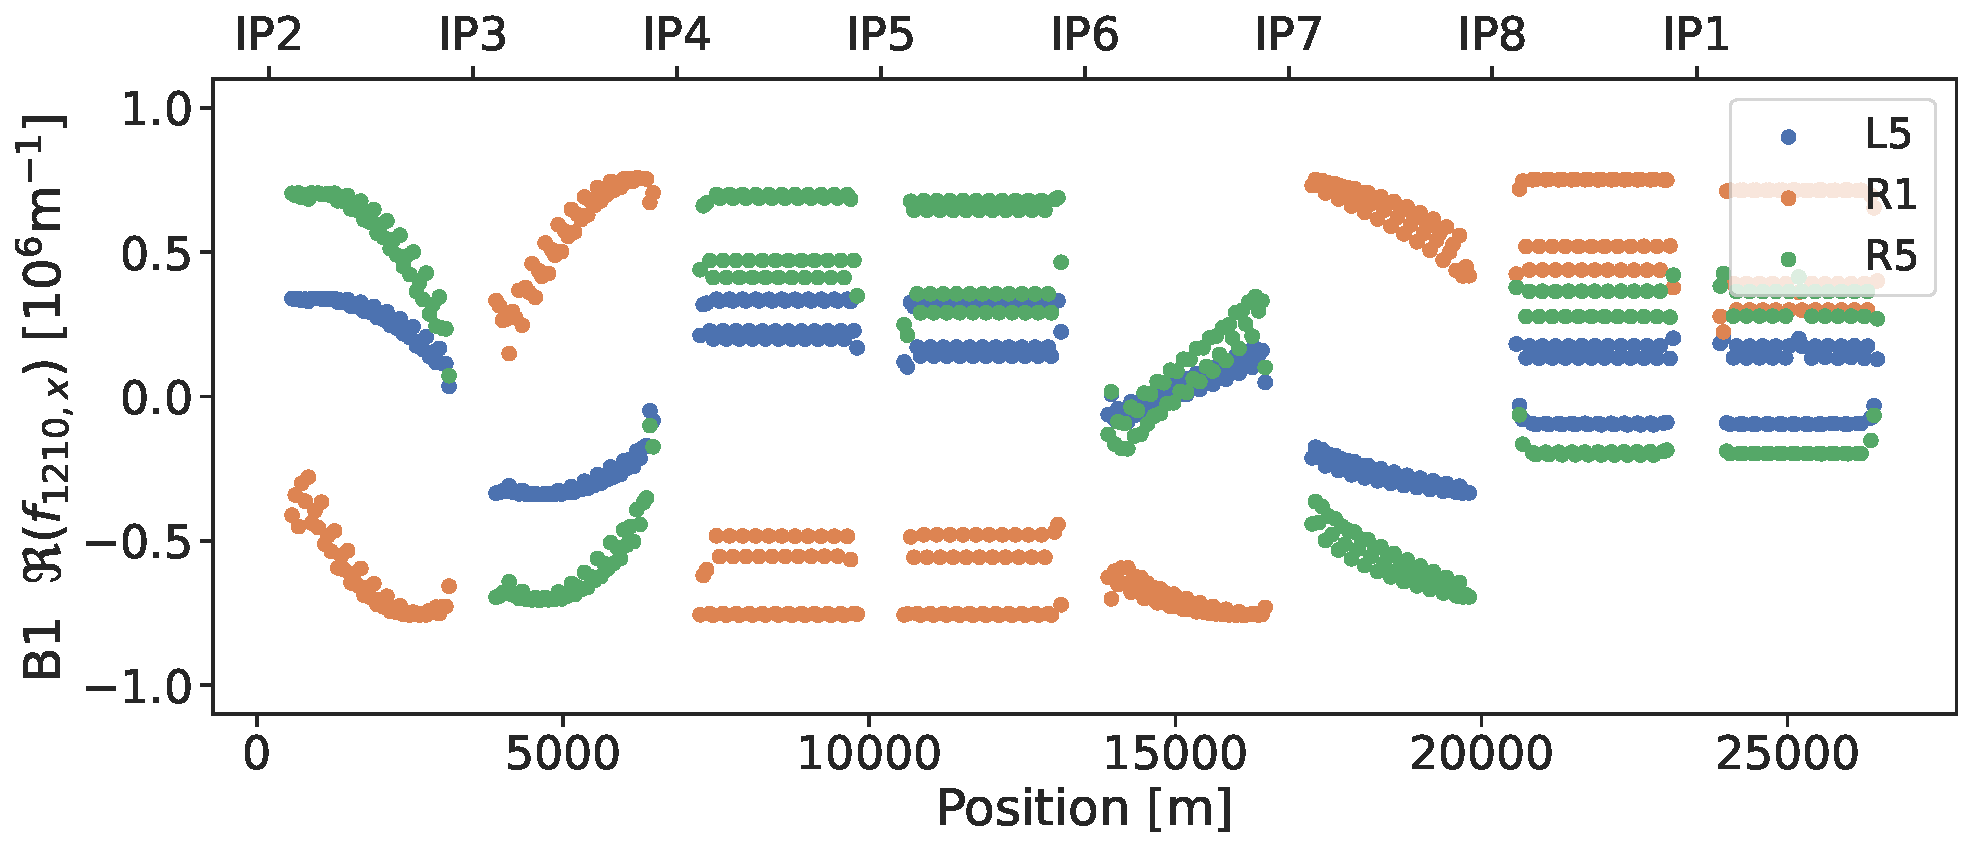
\includegraphics[width=\textwidth]{./images/f1210_b1_correctors.pdf}
        \caption{$f_{1210,x}$}
    \end{subfigure}
    \caption{Simulation of the RDT response of the skew octupolar correctors at top energy for Beam
    1. Each corrector is powered at $J_4 = 1 [\text{m}^{-4}]$.}
    \label{fig:skew_octupolar:response_correctors}
\end{figure}

It can already be seen that the L5 and R5 correctors show a similar trend along the ring, with L5
showing a stronger response for the same strength, while the R1 corrector follows the opposite
trend. A polar plot at a given BPM can illustrate that trend, and be used to get an intuition of the
effect of the correctors to manually compute corrections.
\Cref{fig:skew_octupolar:response_correctors_polar} shows the orthogonality of the correctors for
both beams and RDTs. L5 being stronger than R5 while having the same angle indicates that only one
of them is needed for corrections. 

\begin{figure}[!htb]
    \centering
    \begin{subfigure}{0.8\textwidth}
        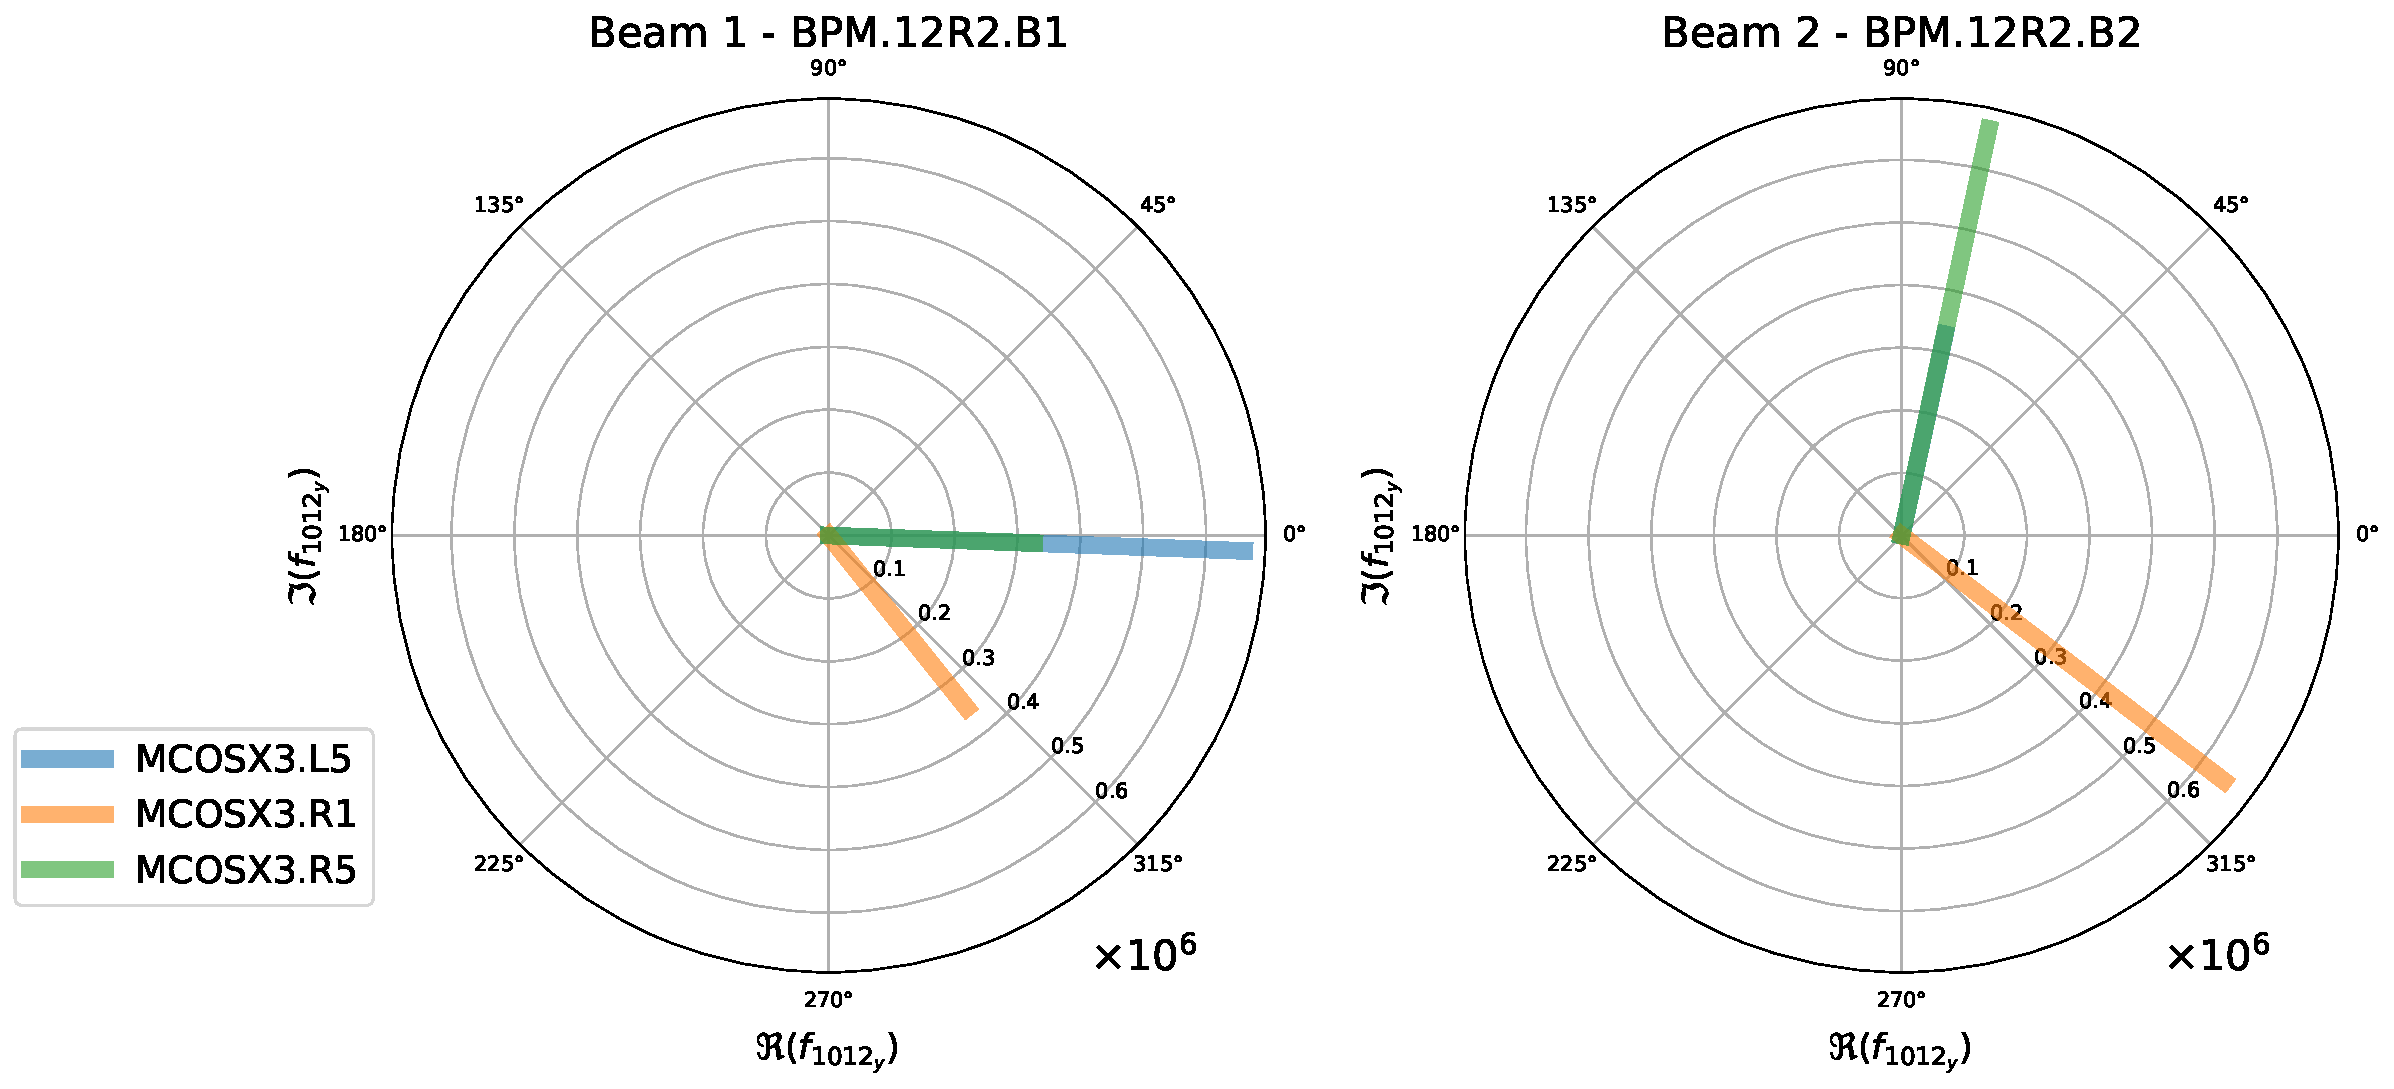
\includegraphics[width=\textwidth]{./images/orthogonal_a4_inj_f1012_y.pdf}
        \caption{$f_{1012,y}$}
    \end{subfigure}
    \par\bigskip 
    \begin{subfigure}{0.8\textwidth}
        \includegraphics[width=\textwidth]{./images/orthogonal_a4_inj_f1210_x.pdf}
        \caption{$f_{1210,x}$}
    \end{subfigure}
    \caption{Simulated RDTs response of the available skew octupolar correctors at top energy.  Each
    corrector is powered at $J_4 = 1 [\text{m}^{-4}]$. The orthogonality of R1 and L5/R5 allows to
    independently control the real and imaginary parts.}
    \label{fig:skew_octupolar:response_correctors_polar}
\end{figure}



%-----------------------------
%         Correction
%-----------------------------
\subsection{\review{Measurements and Corrections}}

Initial measurements of the machine at top energy ($\beta^*=30$cm) without any skew octupolar
correctors were done during an MD slot in 2022 to determine the level of the RDTs before being able
to correct them. Those measurements were made at natural tunes of $Q_x = 0.285$ and $Q_y = 0.292$.
The driven tunes were set to $\Delta Q_x = -0.008$ and $\Delta Q_y = 0.01$. This selection of tunes
has proven to be appropriate for measuring skew octupolar RDTs. The Landau octupoles were powered
off during the measurements. 

The corrections were computed via the previously detailed response matrix and are shown in
\cref{tab:skew_octupolar:correction_strengths}. These have then been applied during 2023's
commissioning and later on kept for operation. The RDT levels of the bare machine and with these
corrections are shown in \cref{fig:skew_octupolar:corrections_vs_bare}. It can be observed that both
RDT amplitudes are reduced, with the exception of $f_{1210,x}$ for Beam 2, which stays constant.
The reduction of RDT amplitude is comparable to those obtained in 2018, where the same RDT for Beam
2 did neither improve or worsen.


\begin{table}[!htb]
    \centering
    \begin{tabular}{lr}
      \toprule
      Corrector    &    Strength $[\text{m}^{-4}]$ \\
      \midrule
      MCOSX3.L1    &                —  \\
      MCOSX3.R1    &           $-0.50$ \\
      MCOSX3.L5    &           $ 0.42$ \\
      MCOSX3.R5    &           $-0.01$ \\
      \bottomrule
    \end{tabular}
    \caption{Computed corrections for skew octupolar RDTs at top energy. The corrector L1 has been 
    broken for several years and can not be used.}
    \label{tab:skew_octupolar:correction_strengths}
\end{table}
 
\begin{figure}[!htb]
    \centering
    \begin{subfigure}{0.49\textwidth}
        \includegraphics[width=\textwidth]{./images/f1012_b1.pdf}
        \caption{$f_{1012,y}$ Beam 1}
    \end{subfigure}
    \hfill
    \begin{subfigure}{0.49\textwidth}
        \includegraphics[width=\textwidth]{./images/f1012_b2.pdf}
        \caption{$f_{1012,y}$ Beam 2}
    \end{subfigure}
    %
    \par\bigskip 
    % 
    \begin{subfigure}{0.49\textwidth}
        \includegraphics[width=\textwidth]{./images/f1210_b1.pdf}
        \caption{$f_{1210,x}$ Beam 1}
    \end{subfigure}
    \hfill
    \begin{subfigure}{0.49\textwidth}
        \includegraphics[width=\textwidth]{./images/f1210_b2.pdf}
        \caption{$f_{1210,x}$ Beam 2}
    \end{subfigure}
    \caption{Measured skew octupolar RDTs at top energy and $\beta^*=30\text{cm}$ before and after
    correction. A reduction if observed for all but one RDT in Beam 2.} 
    \label{fig:skew_octupolar:corrections_vs_bare}
\end{figure}






%=============================
%    Landau Contribution
%=============================
% https://indico.cern.ch/event/1351567/contributions/5708754/attachments/2773145/4832599/2023-12-15_MO_Roll_Coupling_complete.pdf
\FloatBarrier
\section{\review{Landau Octupoles Contribution}}


%-----------------------------
%        Introduction
%-----------------------------
\subsection{\review{Introduction}}

During the 2023 commissioning, measurements were taken at injection energy with different strengths
of Landau octupoles, where an unexpected shift in the skew octupolar RDTs was observed. Subsequent
measurements were conducted to better understand and characterize this contribution of normal
octupoles to skew octupolar fields. These new measurements were taken during an MD slot in September
2023 and focused on varying the strengths of the Landau octupoles to $-1K_4$, $\pm2 K_4$, $5K_4$.
All measurements were taken at injection energy at tunes of $Q_x = 0.275$, $Q_y = 0.293$ and
AC-Dipole deltas of $\Delta Q_x = -0.01$ and $\Delta Q_y = -0.011$. Although both beams were
measured, this section focuses on Beam 1 to preliminarily investigate the matter.  The following
\cref{fig:skew_octupolar:mo_different_levels_meas} illustrates the difference in amplitude of the
RDT $f_{1012}$ with these varying strengths.
\Cref{fig:skew_octupolar:mo_meas_vs_sim_+2} on the other hand shows the measured and simulated shift
of the same RDT from $0K_4$ to $+2K_4$. It is evident that simulations including normal and skew 
octupolar field errors are not enough to explain the behaviour observed in the measurements.

\begin{figure}[!htb]
    \centering
    \begin{subfigure}{0.8\textwidth}
        \includegraphics[width=\textwidth]{./images/skew_octupoles/f1210_AMP_all_measurements.pdf}
    \end{subfigure}
    \caption{Unexpected difference of skew octupolar RDT amplitudes with varying Landau octupoles
    strengths.}
    \label{fig:skew_octupolar:mo_different_levels_meas}
\end{figure}

\begin{figure}[!htb]
    \centering
    \begin{subfigure}{0.8\textwidth}
        \includegraphics[width=\textwidth]{./images/skew_octupoles/f1012_meas_vs_sim_0shift.pdf}
        %\caption{$f_{1012,y}$}
    \end{subfigure}
    \caption{Measured and simulated shift of skew octupolar RDT after increase of Landau octupoles
    strength from zero. It is apparent that the shift in measurement is not replicated by the
    simulation.}
    \label{fig:skew_octupolar:mo_meas_vs_sim_+2}
\end{figure}



%-----------------------------
%        Misalignments
%-----------------------------
\subsection{\review{Misalignments}}

Magnet misalignments, more specifically roll errors, can generate skew magnetic fields instead of
the expected normal ones. To determine if this could explain the behaviour observed in measurements,
a tracking simulation was conducted with and without roll errors applied to the Landau octupoles.
The resulting RDTs reveal an imperceptible difference, unable to account for  the previously seen
shifts. The real part of the RDT $f_{1012}$ is shown in \cref{fig:skew_octupolar:sim_misalign},
with similar results seen in the other component and in $f_{1210}$.

\begin{figure}[!htb]
    \centering
    \begin{subfigure}{0.8\textwidth}
        \includegraphics[width=\textwidth]{./images/skew_octupoles/f1012_misalign_REAL.pdf}
        %\caption{$f_{1012,y}$}
    \end{subfigure}
    \caption{Simulated skew octupolar RDT with normal and skew octupolar errors and Landau octupoles
    powered. One simulation includes further alignment errors on the Landau octupoles. No 
    significant difference is observed between the two.}
    \label{fig:skew_octupolar:sim_misalign}
\end{figure}



%-----------------------------
%        Coupling
%-----------------------------
\subsection{\review{Coupling}}

As misalignments could not explain the discrepancy, simulations were first run with varying values
of coupling at a fixed octupolar strength, allowing to gage the impact of coupling only.
\Cref{appendix:transfer_map:skew_quadrupole_and_octupole} details how coupling, in the form of a
skew quadrupole, combined with a normal octupole can generate skew quadrupolar-like fields.
The resulting RDT $f_{1012}$ is shown in \cref{fig:skew_octupolar:sim_coupling}, a similar trend is
observed for $f_{1210}$.
The presented $C^{-}$ values are commonly seen in operation and well below that of the
tolerances of the design of the LHC~\cite{bruning_lhc_2004}. As coupling increases, the skew
octupolar RDTs are expected to be significantly altered.

\begin{figure}[!htb]
    \centering
    \begin{subfigure}{0.8\textwidth}
        \includegraphics[width=\textwidth]{./images/skew_octupoles/f1012_coupling_sim_AMP.pdf}
    \end{subfigure}
    \caption{Simulated skew octupolar RDT with fixed Landau octupole strength but varying coupling.
    Selected coupling values are often seen in operation.}
    \label{fig:skew_octupolar:sim_coupling}
\end{figure}



%-----------------------------
%          Responses
\FloatBarrier
\subsubsection{\review{Responses with Coupling}}

\begin{table}[!htb]
    \centering
    \begin{tabular}{cccc}
    \toprule
    &&\multicolumn{2}{c}{Rel. Diff. [\%]} \\
    \cmidrule{3-4}
    $K_4$ $[\text{m}^{-4}]$ & RDT & Real & Imag. \\
    \midrule
    \multirow{2}{*}{+5}
     & $f_{1210}$ & 6 & 6  \\
     & $f_{1012}$ & 12  & 11 \\[0.5em]
    \multirow{2}{*}{+2}
     & $f_{1210}$ & 32  & 34  \\
     & $f_{1012}$ & 36  & 36  \\[0.5em]
    \multirow{2}{*}{-1}
     & $f_{1210}$ & 26 & 25 \\
     & $f_{1012}$ & 21 & 20 \\[0.5em]
    \multirow{2}{*}{-2}
     & $f_{1210}$ & 19  & 17  \\
     & $f_{1012}$ & 21 & 20 \\
    \bottomrule
    \end{tabular}
    \caption{Relative difference between measured and simulated RDT shift induced by the
    Landau octupoles in presence of coupling. Real parts are illustrated in
    \cref{fig:skew_octupolar:response_meas_sim_coupling}.}
    \label{tab:skew_octupolar:rms_ratios}
\end{table}

After having demonstrated that coupling could significantly contribute to the creation of skew
octupolar fields with normal octupoles, additional simulations were performed matching the measured
coupling for each set of measurements. The shift in real part of the RDTs $f_{1012}$ and $f_{1210}$
is shown in \cref{fig:skew_octupolar:response_meas_sim_coupling}, with a similar pattern observed
for the imaginary part. The relative RMS deviation between simulations and measurements is given
for each set of strengths and RDTs in \cref{tab:skew_octupolar:rms_ratios}.

It can be observed that simulations and measurements for positive strengths ($K_4=2$ and $K_4=5$) 
are now in good agreement. This suggests that the primary contribution to the skew octupolar RDTs
can be attributed to the Landau octupoles and coupling. The relative deviation between measurement
and simulation can be explained by the sensitivity to the coupling. A difference of $10^{-4}$ units 
is enough to be noticeable, making accurate reproduction of skew octupolar RDTs not trivial.
It is important to note that measurements of $f_{1012}$ with \textit{negative} strength show a
response opposite to what is predicted by simulations while $f_{1210}$ agrees well. This behaviour
is not yet understood and requires further investigation.

\begin{figure}[!htb]
    \centering
    \begin{subfigure}{0.47\textwidth}
        \includegraphics[width=\textwidth]{./images/skew_octupoles/responses_coupling/f1012_response_meas_sim_+5_REAL_smoll.pdf}
        %\caption{$f_{1012,y}$ for $K_4 = +5$}
    \end{subfigure}
    \hfill
    \begin{subfigure}{0.47\textwidth}
        \includegraphics[width=\textwidth]{./images/skew_octupoles/responses_coupling/f1210_response_meas_sim_+5_REAL_smoll.pdf}
        %\caption{$f_{1210,x}$ for $K_4 = +5$}
    \end{subfigure}
    %
    \par\medskip 
    %
    \begin{subfigure}{0.47\textwidth}
        \includegraphics[width=\textwidth]{./images/skew_octupoles/responses_coupling/f1012_response_meas_sim_+2_REAL_smoll.pdf}
        %\caption{$f_{1012,y}$ for $K_4 = +2$}
    \end{subfigure}
    \hfill
    \begin{subfigure}{0.47\textwidth}
        \includegraphics[width=\textwidth]{./images/skew_octupoles/responses_coupling/f1210_response_meas_sim_+2_REAL_smoll.pdf}
        %\caption{$f_{1210,x}$ for $K_4 = +2$}
    \end{subfigure}
    %
    \par\medskip 
    %
    \begin{subfigure}{0.47\textwidth}
        \includegraphics[width=\textwidth]{./images/skew_octupoles/responses_coupling/f1012_response_meas_sim_-1_REAL_smoll.pdf}
        %\caption{$f_{1012,y}$ for $K_4 = -1$}
    \end{subfigure}
    \hfill
    \begin{subfigure}{0.47\textwidth}
        \includegraphics[width=\textwidth]{./images/skew_octupoles/responses_coupling/f1210_response_meas_sim_-1_REAL_smoll.pdf}
        %\caption{$f_{1210,x}$ for $K_4 = -1$}
    \end{subfigure}
    %
    \par\medskip
    %
    \begin{subfigure}{0.47\textwidth}
        \includegraphics[width=\textwidth]{./images/skew_octupoles/responses_coupling/f1012_response_meas_sim_-2_REAL_smoll.pdf}
        %\caption{$f_{1012,y}$ for $K_4 = -2$}
    \end{subfigure}
    \hfill
    \begin{subfigure}{0.47\textwidth}
        \includegraphics[width=\textwidth]{./images/skew_octupoles/responses_coupling/f1210_response_meas_sim_-2_REAL_smoll.pdf}
        %\caption{$f_{1210,x}$ for $K_4 = -2$}
    \end{subfigure}
    \caption{Measured and simulated real part shift of skew octupolar RDTs induced by Landau
    octupoles in presence of coupling at injection energy. Left column shows $f_{1012}$ while right
    shows $f_{1210}$. The vertical scale is adjusted for each plot to highlight the agreement of the 
    simulations.}
    \label{fig:skew_octupolar:response_meas_sim_coupling}
\end{figure}


% Imaginary Parts
%\begin{figure}[!htb]
%    \centering
%    \begin{subfigure}{0.47\textwidth}
%        \includegraphics[width=\textwidth]{./images/skew_octupoles/responses_coupling/f1012_response_meas_sim_+5_IMAG_smoll.pdf}
%        %\caption{$f_{1012,y}$ for $K_4 = +5$}
%    \end{subfigure}
%    \hfill
%    \begin{subfigure}{0.47\textwidth}
%        \includegraphics[width=\textwidth]{./images/skew_octupoles/responses_coupling/f1210_response_meas_sim_+5_IMAG_smoll.pdf}
%        %\caption{$f_{1210,x}$ for $K_4 = +5$}
%    \end{subfigure}
%    %
%    \par\medskip 
%    %
%    \begin{subfigure}{0.47\textwidth}
%        \includegraphics[width=\textwidth]{./images/skew_octupoles/responses_coupling/f1012_response_meas_sim_+2_IMAG_smoll.pdf}
%        %\caption{$f_{1012,y}$ for $K_4 = +2$}
%    \end{subfigure}
%    \hfill
%    \begin{subfigure}{0.47\textwidth}
%        \includegraphics[width=\textwidth]{./images/skew_octupoles/responses_coupling/f1210_response_meas_sim_+2_IMAG_smoll.pdf}
%        %\caption{$f_{1210,x}$ for $K_4 = +2$}
%    \end{subfigure}
%    %
%    \par\medskip 
%    %
%    \begin{subfigure}{0.47\textwidth}
%        \includegraphics[width=\textwidth]{./images/skew_octupoles/responses_coupling/f1012_response_meas_sim_-1_IMAG_smoll.pdf}
%        %\caption{$f_{1012,y}$ for $K_4 = -1$}
%    \end{subfigure}
%    \hfill
%    \begin{subfigure}{0.47\textwidth}
%        \includegraphics[width=\textwidth]{./images/skew_octupoles/responses_coupling/f1210_response_meas_sim_-1_IMAG_smoll.pdf}
%        %\caption{$f_{1210,x}$ for $K_4 = -1$}
%    \end{subfigure}
%    %
%    \par\medskip
%    %
%    \begin{subfigure}{0.47\textwidth}
%        \includegraphics[width=\textwidth]{./images/skew_octupoles/responses_coupling/f1012_response_meas_sim_-2_IMAG_smoll.pdf}
%        %\caption{$f_{1012,y}$ for $K_4 = -2$}
%    \end{subfigure}
%    \hfill
%    \begin{subfigure}{0.47\textwidth}
%        \includegraphics[width=\textwidth]{./images/skew_octupoles/responses_coupling/f1210_response_meas_sim_-2_IMAG_smoll.pdf}
%        %\caption{$f_{1210,x}$ for $K_4 = -2$}
%    \end{subfigure}
%    \caption{Measured and simulated imaginary part shift of skew octupolar RDTs induced by Landau
%    octupoles in presence of coupling at injection energy. Left column shows $f_{1012}$ while right
%    shows $f_{1210}$.}
%    \label{fig:skew_octupolar:response_meas_sim_coupling_imag}
%\end{figure}


% Constant coupling
%\begin{figure}[!htb]
%    \centering
%    \begin{subfigure}{0.47\textwidth}
%        \includegraphics[width=\textwidth]{./images/skew_octupoles/responses_coupling/f1012_response_meas_sim_+5_REAL_smoll_const_coupling.pdf}
%        %\caption{$f_{1012,y}$ for $K_4 = +5$}
%    \end{subfigure}
%    \hfill
%    \begin{subfigure}{0.47\textwidth}
%        \includegraphics[width=\textwidth]{./images/skew_octupoles/responses_coupling/f1210_response_meas_sim_+5_REAL_smoll_const_coupling.pdf}
%        %\caption{$f_{1210,x}$ for $K_4 = +5$}
%    \end{subfigure}
%    %
%    \par\medskip 
%    %
%    \begin{subfigure}{0.47\textwidth}
%        \includegraphics[width=\textwidth]{./images/skew_octupoles/responses_coupling/f1012_response_meas_sim_+2_REAL_smoll_const_coupling.pdf}
%        %\caption{$f_{1012,y}$ for $K_4 = +2$}
%    \end{subfigure}
%    \hfill
%    \begin{subfigure}{0.47\textwidth}
%        \includegraphics[width=\textwidth]{./images/skew_octupoles/responses_coupling/f1210_response_meas_sim_+2_REAL_smoll_const_coupling.pdf}
%        %\caption{$f_{1210,x}$ for $K_4 = +2$}
%    \end{subfigure}
%    %
%    \par\medskip 
%    %
%    \begin{subfigure}{0.47\textwidth}
%        \includegraphics[width=\textwidth]{./images/skew_octupoles/responses_coupling/f1012_response_meas_sim_-1_REAL_smoll_const_coupling.pdf}
%        %\caption{$f_{1012,y}$ for $K_4 = -1$}
%    \end{subfigure}
%    \hfill
%    \begin{subfigure}{0.47\textwidth}
%        \includegraphics[width=\textwidth]{./images/skew_octupoles/responses_coupling/f1210_response_meas_sim_-1_REAL_smoll_const_coupling.pdf}
%        %\caption{$f_{1210,x}$ for $K_4 = -1$}
%    \end{subfigure}
%    %
%    \par\medskip
%    %
%    \begin{subfigure}{0.47\textwidth}
%        \includegraphics[width=\textwidth]{./images/skew_octupoles/responses_coupling/f1012_response_meas_sim_-2_REAL_smoll_const_coupling.pdf}
%        %\caption{$f_{1012,y}$ for $K_4 = -2$}
%    \end{subfigure}
%    \hfill
%    \begin{subfigure}{0.47\textwidth}
%        \includegraphics[width=\textwidth]{./images/skew_octupoles/responses_coupling/f1210_response_meas_sim_-2_REAL_smoll_const_coupling.pdf}
%        %\caption{$f_{1210,x}$ for $K_4 = -2$}
%    \end{subfigure}
%    \caption{Measured and simulated real part shift of skew octupolar RDTs induced by Landau
%    octupoles in presence of coupling at injection energy. Left column shows $f_{1012}$ while right
%    shows $f_{1210}$.}
%    \label{fig:skew_octupolar:response_meas_sim_coupling}
%\end{figure}
%
%
%% Imaginary Parts
%\begin{figure}[!htb]
%    \centering
%    \begin{subfigure}{0.47\textwidth}
%        \includegraphics[width=\textwidth]{./images/skew_octupoles/responses_coupling/f1012_response_meas_sim_+5_IMAG_smoll_const_coupling.pdf}
%        %\caption{$f_{1012,y}$ for $K_4 = +5$}
%    \end{subfigure}
%    \hfill
%    \begin{subfigure}{0.47\textwidth}
%        \includegraphics[width=\textwidth]{./images/skew_octupoles/responses_coupling/f1210_response_meas_sim_+5_IMAG_smoll_const_coupling.pdf}
%        %\caption{$f_{1210,x}$ for $K_4 = +5$}
%    \end{subfigure}
%    %
%    \par\medskip 
%    %
%    \begin{subfigure}{0.47\textwidth}
%        \includegraphics[width=\textwidth]{./images/skew_octupoles/responses_coupling/f1012_response_meas_sim_+2_IMAG_smoll_const_coupling.pdf}
%        %\caption{$f_{1012,y}$ for $K_4 = +2$}
%    \end{subfigure}
%    \hfill
%    \begin{subfigure}{0.47\textwidth}
%        \includegraphics[width=\textwidth]{./images/skew_octupoles/responses_coupling/f1210_response_meas_sim_+2_IMAG_smoll_const_coupling.pdf}
%        %\caption{$f_{1210,x}$ for $K_4 = +2$}
%    \end{subfigure}
%    %
%    \par\medskip 
%    %
%    \begin{subfigure}{0.47\textwidth}
%        \includegraphics[width=\textwidth]{./images/skew_octupoles/responses_coupling/f1012_response_meas_sim_-1_IMAG_smoll_const_coupling.pdf}
%        %\caption{$f_{1012,y}$ for $K_4 = -1$}
%    \end{subfigure}
%    \hfill
%    \begin{subfigure}{0.47\textwidth}
%        \includegraphics[width=\textwidth]{./images/skew_octupoles/responses_coupling/f1210_response_meas_sim_-1_IMAG_smoll_const_coupling.pdf}
%        %\caption{$f_{1210,x}$ for $K_4 = -1$}
%    \end{subfigure}
%    %
%    \par\medskip
%    %
%    \begin{subfigure}{0.47\textwidth}
%        \includegraphics[width=\textwidth]{./images/skew_octupoles/responses_coupling/f1012_response_meas_sim_-2_IMAG_smoll_const_coupling.pdf}
%        %\caption{$f_{1012,y}$ for $K_4 = -2$}
%    \end{subfigure}
%    \hfill
%    \begin{subfigure}{0.47\textwidth}
%        \includegraphics[width=\textwidth]{./images/skew_octupoles/responses_coupling/f1210_response_meas_sim_-2_IMAG_smoll_const_coupling.pdf}
%        %\caption{$f_{1210,x}$ for $K_4 = -2$}
%    \end{subfigure}
%    \caption{Measured and simulated imaginary part shift of skew octupolar RDTs induced by Landau
%    octupoles in presence of coupling at injection energy. Left column shows $f_{1012}$ while right
%    shows $f_{1210}$.}
%    \label{fig:skew_octupolar:response_meas_sim_coupling_imag}
%\end{figure}


%=============================
%        Conclusion
%=============================
\FloatBarrier
\section{\review{Summary}}


This chapter investigates the origins of skew octupolar fields in the LHC and explores methods to
mitigate their effects. Previous studies have shown that these fields significantly contribute to
limitations in dynamic aperture, particularly when the beam is kicked with the AC-Dipole. The skew
octupolar correctors, located around the ATLAS and CMS detectors, are crucial for managing these
fields.

A response matrix method was developed to correct skew octupolar RDTs at top energy using the
available corrector magnets. While effective, the absence of one corrector limits the achievable
correction strength. As a result, the RDTs $f_{1012}$ and $f_{1210}$ are either successfully
corrected or maintained at a constant level.

Additionally, this chapter addresses the unexpected influence of Landau octupoles on skew octupolar
RDTs at injection energy. Simulations reveal that misalignments of the Landau octupoles,
specifically roll errors, do not a have a significant impact. Instead, coupling was found to be a
crucial factor.  While further investigation is required to fully understand the underlying
mechanisms, initial findings suggest that accurate modeling of coupling is essential for predicting
the behavior of skew octupolar RDTs in the presence of Landau octupoles. During regular operation,
where the Landau octupoles are powered at $K_4=18$, very large skew octupolar RDTs are expected to
be generated.

The results presented provide valuable insights into the complex interplay of
magnetic fields in the LHC and highlight the importance of accurate modeling for corrections.


% =================================================
%                    Appendices
% =================================================

\appendix  % Declare we started the appendix, that switches the numbering to letters


% ==============================================================
%                      Units and Conversions
% ==============================================================
\chapter{Units and Conversions}
\thumbforappendix


% ---------------------------------------
%          Units and Conversions
% ---------------------------------------
\section{Physical Constants}

\begin{table}[H]
    \centering
    \begin{tabular}{lcrl}
    Name                        &    Symbol     &    Value                        &     Unit      \\
    Speed of light in vacuum    &     $c$       &   $2.99792458 \times 10^8$      &      m/s      \\
    Elementary charge           &     $e$       &   $1.60217663 \times 10^9$      &       C       \\
        
    \end{tabular}
    \caption{Physical Constants}
    \label{table:appendix:physical_constants}
\end{table}


\section{Units}


\section{Conversions}


% ==============================================================
%                 Hamiltonians and Transfer Maps
% ==============================================================
\chapter{Hamiltonians and Transfer Maps}
\label{appendix:transfer_maps}
\thumbforappendix

This appendix is intended to gather and explicit the Hamiltonians of the elements used in this 
thesis. Non-linear transfer maps are also described for some of those elements from the first to
the second order.

% ---------------------------------------
%              Hamiltonians
% ---------------------------------------
\section{Hamiltonians of Elements}

The Hamiltonian of a \textit{multipole} is the
following~\cite{keintzel_jacqueline_beam_nodate,tomas_direct_2003,franchi_studies_2006}:

\begin{equation}
    H = \Re \left[ \sum_{n>1} (K_n + iJ_n) \frac{(x+iy)^n}{n!} \right].
\end{equation}

From this, normal and skew fields can be separated:

\begin{equation}
    \begin{aligned}
        N_n &= \frac{1}{n!} K_n \Re \left[ (x+iy)^n \right] \\
        S_n &= -\frac{1}{n!} J_n \Im \left[ (x+iy)^n \right],
    \end{aligned}
\end{equation}

where $K$ and $J$ are the normalized strength of the multipole and $x,y$ the transverse coordinates.

\cref{table:appendix:hamiltonians} explicits the normal and skew Hamiltonians of multipoles up to
order 8.

\begin{table}[H]
    \centering
    \begin{tabular}{l  c  p{7.8cm}}
      \hline
       Name & Order & Normal and Skew Hamiltonians\\
      \hline
      \midrule
        Drift          & - & $H = \frac{1}{2} (p_x^2 + p_y^2)$ \\
      \midrule
        Dipole         & 1 & $N_1 = K_{1} x$                                                                                            \newline $S_1 = - J_{1} y$ \\
      \midrule
        Quadrupole     & 2 & $N_2 = \frac{1}{2!} K_{2} \left(x^{2} - y^{2}\right)$                                                       \newline $S_2 = - J_{2} x y$ \\
      \midrule
        Sextupole      & 3 & $N_3 = \frac{1}{3!}K_{3} \left(x^{3} - 3 x y^{2}\right)$                                                    \newline $S_3 = - \frac{1}{3!}J_{3} \cdot \left(3 x^{2} y - y^{3}\right)$ \\
      \midrule
        Octupole       & 4 & $N_4 = \frac{1}{4!}K_{4} \left(x^{4} - 6 x^{2} y^{2} + y^{4}\right)$                                       \newline $S_4 = - \frac{1}{4!}J_{4} \cdot \left(4 x^{3} y - 4 x y^{3}\right)$ \\
      \midrule
        Decapole       & 5 & $N_5 = \frac{1}{5!}K_{5} \left(x^{5} - 10 x^{3} y^{2} + 5 x y^{4}\right)$                                 \newline $S_5 = - \frac{1}{5!}J_{5} \cdot \left(5 x^{4} y - 10 x^{2} y^{3} + y^{5}\right)$ \\
      \midrule
        Dodecapole     & 6 & $N_6 = \frac{1}{6!}K_{6} \left(x^{6} - 15 x^{4} y^{2} + 15 x^{2} y^{4} - y^{6}\right)$                    \newline $S_6 = - \frac{1}{6!}J_{6} \cdot \left(6 x^{5} y - 20 x^{3} y^{3} + 6 x y^{5}\right)$ \\
      \midrule
        Decatetrapole  & 7 & $N_7 = \frac{1}{7!}K_{7} \left(x^{7} - 21 x^{5} y^{2} + 35 x^{3} y^{4} - 7 x y^{6}\right)$               \newline $S_7 = - \frac{1}{7!}J_{7} \cdot \left(7 x^{6} y - 35 x^{4} y^{3} + 21 x^{2} y^{5} - y^{7}\right)$ \\
      \midrule
        Decahexapole   & 8 & $N_8 = \frac{1}{8!}K_{8} \left(x^{8} - 28 x^{6} y^{2} + 70 x^{4} y^{4} - 28 x^{2} y^{6} + y^{8}\right)$ \newline $S_8 = - \frac{1}{8!}J_{8} \cdot \left(8 x^{7} y - 56 x^{5} y^{3} + 56 x^{3} y^{5} - 8 x y^{7}\right)$ \\
      \midrule
      \end{tabular}
  \caption{Normal and skew Hamiltonians of multipoles up to order 8.}
  \label{table:appendix:hamiltonians}
\end{table}



% ---------------------------------------
%             Transfer Maps
% ---------------------------------------
\section{Transfer Maps}

Two sextupoles to the second order:
\footnotesize
\begin{equation}
    \begin{aligned}
      Z = &\left.
      K_{3,h1} K_{3,h2} L_{1} L_{2} L_{D} \left(
      %
      \begin{aligned}
        &\frac{L_{D}^{2} p_{x}^{2} x^{2}}{8} - \frac{L_{D}^{2} p_{x}^{2} y^{2}}{8} + \frac{L_{D}^{2} p_{x} p_{y} x y}{2} - \frac{L_{D}^{2} p_{y}^{2} x^{2}}{8} \\
        &+ \frac{L_{D}^{2} p_{y}^{2} y^{2}}{8} + \frac{L_{D} p_{x} x^{3}}{4} + \frac{L_{D} p_{x} x y^{2}}{4} + \frac{L_{D} p_{y} x^{2} y}{4} \\
        &+ \frac{L_{D} p_{y} y^{3}}{4} + \frac{x^{4}}{8} + \frac{x^{2} y^{2}}{4} + \frac{y^{4}}{8}
      \end{aligned} \right) \;\,\right\} \; \text{octupolar-like terms}\\
      %
      & \left.
      \begin{aligned}
        &+ K_{3,h1} L_{1} L_{D} \left(
        %
        \begin{aligned}
          &\frac{L_{D}^{2} p_{x}^{3}}{6} - \frac{L_{D}^{2} p_{x} p_{y}^{2}}{2} + \frac{L_{D} p_{x}^{2} x}{2} \\
          &- L_{D} p_{x} p_{y} y - \frac{L_{D} p_{y}^{2} x}{2} + \frac{p_{x} x^{2}}{2} - \frac{p_{x} y^{2}}{2} - p_{y} x y
        \end{aligned}\right)\\
        %
        &+ K_{3,h1} L_{1} \left(\frac{x^{3}}{6} - \frac{x y^{2}}{2}\right) + K_{3,H2} L_{2} \left(\frac{x^{3}}{6} - \frac{x y^{2}}{2}\right)
      \end{aligned}
      \qquad\quad\right\} \; \text{sextupolar terms}
    \end{aligned}
\end{equation}
\normalsize



Two sextupoles to the third order:
\footnotesize
\begin{equation}
  \begin{aligned}
    \\[7em]
    Z =
      %
      %
      % Decapole terms
      \\[-9.7em]
      &\left.
      \begin{aligned}
      &K_{3,h1}^{2} K_{3,h2} L_{1}^{2} L_{2} L_{D} \left(
     \begin{aligned}
       &\frac{L_{D}^{5} p_{x}^{4} x}{48} + \frac{L_{D}^{5} p_{x}^{3} p_{y} y}{12} - \frac{L_{D}^{5} p_{x}^{2} p_{y}^{2} x}{8} - \frac{L_{D}^{5} p_{x} p_{y}^{3} y}{12} \\
       &+ \frac{L_{D}^{5} p_{y}^{4} x}{48} + \frac{L_{D}^{4} p_{x}^{3} x^{2}}{12} + \frac{L_{D}^{4} p_{x}^{3} y^{2}}{12}- \frac{L_{D}^{4} p_{x} p_{y}^{2} x^{2}}{4} \\
       &- \frac{L_{D}^{4} p_{x} p_{y}^{2} y^{2}}{4} + \frac{L_{D}^{3} p_{x}^{2} x^{3}}{8} + \frac{L_{D}^{3} p_{x}^{2} x y^{2}}{8} - \frac{L_{D}^{3} p_{x} p_{y} x^{2} y}{4} \\
       &- \frac{L_{D}^{3} p_{x} p_{y} y^{3}}{4} - \frac{L_{D}^{3} p_{y}^{2} x^{3}}{8} - \frac{L_{D}^{3} p_{y}^{2} x y^{2}}{8} + \frac{L_{D}^{2} p_{x} x^{4}}{12} \\
       &- \frac{L_{D}^{2} p_{x} y^{4}}{12} - \frac{L_{D}^{2} p_{y} x^{3} y}{6} - \frac{L_{D}^{2} p_{y} x y^{3}}{6} + \frac{L_{D} x^{5}}{48} \\
       &- \frac{L_{D} x^{3} y^{2}}{24} - \frac{L_{D} x y^{4}}{16}
     \end{aligned} \right) \\
       %
       %
       % Decapole again
      &+ K_{3,h1} K_{3,h2}^{2} L_{1} L_{2}^{2} L_{D} \left(
      \begin{aligned}
        &\frac{L_{D}^{2} p_{x} x^{4}}{48} - \frac{L_{D}^{2} p_{x} x^{2} y^{2}}{8} + \frac{L_{D}^{2} p_{x} y^{4}}{48} + \frac{L_{D}^{2} p_{y} x^{3} y}{12} \\
        &- \frac{L_{D}^{2} p_{y} x y^{3}}{12} + \frac{L_{D} x^{5}}{48} - \frac{L_{D} x^{3} y^{2}}{24} - \frac{L_{D} x y^{4}}{16}
      \end{aligned}\right)
      \end{aligned}
      \; \right\} \; \text{decapolar-like} \\
      %
      %
      % Octupole terms
      \\[-1.5em]
    &+ K_{3,h1} K_{3,h2} L_{1} L_{2} L_{D} \left. \left(
    \begin{aligned}
      &\frac{L_{D}^{2} p_{x}^{2} x^{2}}{8} - \frac{L_{D}^{2} p_{x}^{2} y^{2}}{8} + \frac{L_{D}^{2} p_{x} p_{y} x y}{2} - \frac{L_{D}^{2} p_{y}^{2} x^{2}}{8} \\
      &+ \frac{L_{D}^{2} p_{y}^{2} y^{2}}{8} + \frac{L_{D} p_{x} x^{3}}{4} + \frac{L_{D} p_{x} x y^{2}}{4} + \frac{L_{D} p_{y} x^{2} y}{4}\\
      &+ \frac{L_{D} p_{y} y^{3}}{4} + \frac{x^{4}}{8} + \frac{x^{2} y^{2}}{4} + \frac{y^{4}}{8}
    \end{aligned} \right)
    \;\; \right\} \; \text{octupolar-like} \\
    %
    %
    % Sextupole
    \\[-1.5em]
    &\left.
    \begin{aligned}
      &+ K_{3,h1} L_{1} L_{D} \left(
      \begin{aligned}
        &\frac{L_{D}^{2} p_{x}^{3}}{6} - \frac{L_{D}^{2} p_{x} p_{y}^{2}}{2} + \frac{L_{D} p_{x}^{2} x}{2} - L_{D} p_{x} p_{y} y \\
        &- \frac{L_{D} p_{y}^{2} x}{2} + \frac{p_{x} x^{2}}{2} - \frac{p_{x} y^{2}}{2} - p_{y} x y
      \end{aligned}\right) \\
      &+ K_{3,h1} L_{1} \left(\frac{x^{3}}{6} - \frac{x y^{2}}{2}\right)
      + K_{3,h2} L_{2} \left(\frac{x^{3}}{6} - \frac{x y^{2}}{2}\right)
  \end{aligned}
  \;\; \right\} \; \text{sextupolar}
  \end{aligned}
  \\
\end{equation}
\normalsize

% ==============================================================
%                    Chromatic Amplitude Detuning
% ==============================================================
\chapter{Chromatic Amplitude Detuning}
\label{chromatic-amplitude-detuning}

This appendix details the derivations of chromatic amplitude detuning from sextupoles up to
dodecapoles. As chromaticity and amplitude detuning are part of it, they will therefore be detailed
here as well.

\newpage
Up to the third order, the expression of the Taylor expansion of the Chromatic Amplitude Detuning
around $\epsilon_x$, $\epsilon_y$ and $\delta$, for a tune $Q_z$, $z \in \{x, y\}$ reads:

\begin{equation}
\begin{aligned}
Q_z(\epsilon_x, \epsilon_y, \delta) = Q_{z0} &+ \left[\frac{\partial Q_z}{\partial \epsilon_x} \epsilon_x
                                                 + \frac{\partial Q_z}{\partial \epsilon_y} \epsilon_y
                                                 + \colorbox{yellow!0}{$\displaystyle \frac{\partial Q_z}{\partial \delta}$} \delta
                                                \right] \\
                                             &+ \frac{1}{2!} \biggl[\frac{\partial^2Q_z}{\partial \epsilon_x^2}\epsilon_x^2 
                                                 + \frac{\partial^2Q_z}{\partial \epsilon_y^2}\epsilon_y^2
                                                 + \colorbox{yellow!0}{$\displaystyle \frac{\partial^2 Q_z}{\partial \delta^2}$} \delta^2  \\
                                             &\;\begin{aligned}
                                             \phantom{+ \frac{1}{2!} \biggl[}
                                               &+ 2 \frac{\partial^2Q_z}{\partial \epsilon_x \partial \epsilon_y}\epsilon_x \epsilon_y
                                                  + 2 \frac{\partial^2Q_z}{\partial \epsilon_x \partial \delta}\epsilon_x \delta
                                                  + 2 \frac{\partial^2Q_z}{\partial \delta \partial \epsilon_y} \delta \epsilon_y
                                             \biggr] \\
                                             \end{aligned} \\
                                             &+ \frac{1}{3!}
                                             \biggl[
                                                  \colorbox{yellow!0}{$\displaystyle \frac{\partial^3 Q_z}{\partial \delta^3}$}\delta^{3}
                                                  + \frac{\partial^{3} Q_z}{\partial \epsilon_{x}^{3}}  \epsilon_{x}^{3} 
                                                  + \frac{\partial^{3} Q_z}{\partial \epsilon_{y}^{3}}  \epsilon_{y}^{3} \\
                                             &\;\begin{aligned}
                                             \phantom{+ \frac{1}{3!} \biggl[} 
                                               &+ 3 \frac{\partial^{3} Q_z}{\partial \epsilon_{x}\partial \delta^{2}} \delta^{2} \epsilon_{x} 
                                                + 3  \frac{\partial^{3} Q_z}{\partial \epsilon_{y}\partial \delta^{2}}  \delta^{2} \epsilon_{y}
                                                + 3 \frac{\partial^{3} Q_z}{\partial \epsilon_{x}^{2}\partial \delta}  \delta \epsilon_{x}^{2} \\
                                               &+ 3 \frac{\partial^{3} Q_z}{\partial \epsilon_{y}^{2}\partial \delta} \delta \epsilon_{y}^{2}  
                                                + 3  \frac{\partial^{3} Q_z}{\partial \epsilon_{y}\partial \epsilon_{x}^{2}} \epsilon_{x}^{2} \epsilon_{y} 
                                                + 3 \frac{\partial^{3} Q_z}{\partial \epsilon_{y}^{2}\partial \epsilon_{x}} \epsilon_{x} \epsilon_{y}^{2} \\
                                               &+ 6 \frac{\partial^{3} Q_z}{\partial \epsilon_{y}\partial  \epsilon_{x}\partial \delta} \delta \epsilon_{x} \epsilon_{y} 
                                             \biggr] + \cdots \\
                                             \end{aligned}
\end{aligned}
\end{equation}


\section{Principle}

From~\cite{dilly_derivation_2023}, the detuning caused by a magnet of length L can be described by
its hamiltonian with 

\begin{equation}
  \Delta Q_z = \frac{1}{2 \pi} \int_L \frac{\partial \langle H \rangle}{\partial J_z} \diff s.
\end{equation}

The usual variables $x$ and $y$ of \cref{eq:normal_skew_hamiltonian_magnet} can be replaced by
\textit{action-angle} variables to introduce the action:

\begin{equation}
  \begin{aligned}
    x \rightarrow \sqrt{2J_x \beta_x} \cos{\phi_x} \\
    y \rightarrow \sqrt{2J_y \beta_y} \cos{\phi_x}
  \end{aligned}
  \label{appendix:chromatic_ampdet:action_angle}
\end{equation}

A momentum dependence can be introduced for a particle with a different orbit
($\Delta z$)~\cite{wiedemann_particle_1999} via dispersion. Combined with
\cref{appendix:chromatic_ampdet:action_angle}, a dependence on all required components is achieved:

\begin{equation}
  \begin{aligned}
    x + \Delta x \rightarrow \sqrt{2J_x \beta_x} \cos{\phi_x} + D_x \delta \\
    y + \Delta y \rightarrow \sqrt{2J_y \beta_y} \cos{\phi_y} + D_y \delta
  \end{aligned}
\end{equation}


After averaging over the phase variable, all that is left is to compute the partial derivatives.

\todo{The following derivations are just copy-paster from old text}

% ======================
\section{Sextupole}

The change of tune induced by a sextupole is:

\begin{equation}Q_x = \frac{1}{4\pi} K_3 \beta_x \eta \delta L\end{equation}
\begin{equation}Q_y = - \frac{1}{4\pi} K_3 \beta_y \eta \delta L\end{equation}

We can now get the terms we're interested in:

\begin{equation}\begin{aligned}
\frac{\partial Q_x}{\partial J_x} = 0 \quad;&& \frac{\partial Q_x}{\partial J_y} = 0 \quad;&& \frac{\partial Q_x}{\partial \delta} = \frac{1}{4\pi}K_3\beta_x\eta L = Q_x'\\
\frac{\partial Q_y}{\partial J_x} = 0 \quad;&& \frac{\partial Q_y}{\partial J_y} = 0 \quad;&& \frac{\partial Q_y}{\partial \delta} = -\frac{1}{4\pi}K_3\beta_y\eta L = Q_y'\\
\end{aligned}\end{equation}

Contribution to the Chromatic Amplitude Detuning:

\begin{equation}
\begin{aligned}
Q_z(\epsilon_x, \epsilon_y, \delta) = \color{gray}Q_{z0} &+ \color{gray}\left[\frac{\partial Q_z}{\partial \epsilon_x} \epsilon_x
                                                 + \frac{\partial Q_z}{\partial \epsilon_y} \epsilon_y
                                                 + \textcolor{orange}{\frac{\partial Q_z}{\partial \delta} \delta}
                                                \right] \\
\end{aligned}
\end{equation}

\newpage

\hypertarget{octupole-2}{%
\subsection{Octupole}\label{octupole-2}}

From the hamiltonian of a normal octupole, with a displacement in \(x\)
(\cref{eq:hamiltonian_displacement_octupole}), we can change the
variable (\(x = \sqrt{2 J_x \beta_x} \cos \phi_x\) and
\(y = \sqrt{2 J_y \beta_y} \cos \phi_y\)):

\begin{equation}
\begin{aligned}
\mathcal{N}_4 = \frac{1}{24} K_4 \biggl[& \left(\sqrt{2J_x\beta_x} cos\phi_x\right)^4 \\
                                        & +4 \left(\sqrt{2 J_x \beta_x} \cos \phi_x\right)^3 \eta \delta \\
                                        & +6 \left(\sqrt{2 J_x \beta_x} \cos \phi_x\right)^2 \eta^2 \delta^2 \\
                                        & +4 \left(\sqrt{2 J_x \beta_x} \cos \phi_x\right) \eta^2 \delta \\
                                        & +\eta^4 \delta^4 \\
                                        & -6 \left(\sqrt{2 J_x \beta_x} \cos \phi_x\right)^2 \left(\sqrt{2 J_y \beta_y}\cos \phi_y\right)^2\\
                                        & -6 \left(\sqrt{2 J_y \beta_y} \cos \phi_y\right)^2 \cdot 2 \left(\sqrt{2 J_x \beta_x}\cos \phi_x\right) \eta \delta \\
                                        & -6 \left(\sqrt{2 J_y \beta_y} \cos \phi_y\right)^2 \eta^2 \delta^2 \\
                                        & + \left(\sqrt{2 J_y \beta_y} \cos \phi_y\right)^4
                                  \biggr]\\
\end{aligned}
\end{equation}

We can now average over the phase variables: \begin{equation}
\begin{aligned}
\left< \mathcal{N}_4 \right> = \frac{1}{24} K_4 \biggl[& \frac{3}{2} J_x^2\beta_x^2 \\
                                                       & +6 J_x \beta_x \eta^2 \delta^2 \\
                                                       & +\eta^4 \delta^4 \\
                                                       & -6 J_x \beta_x J_y \beta_y\\
                                                       & -6 J_y \beta_y \eta^2 \delta^2 \\
                                                       & + \frac{3}{2} J_y^2 \beta_y^2
                                                 \biggr]\\
\end{aligned}
\end{equation}

The tunes then are:

\begin{equation}\begin{aligned}
Q_x = \frac{1}{2\pi} \frac{\partial \left< \mathcal{N_4} \right>}{\partial J_x} &= \frac{1}{48\pi} K_4 \biggl[3 J_x \beta_x^2
                                                                                                             +6 \beta_x \eta^2 \delta^2
                                                                                                             -6 \beta_x J_y  \beta_y 
                                                                                                      \biggr]\\
Q_y = \frac{1}{2\pi} \frac{\partial \left< \mathcal{N_4} \right>}{\partial J_y} &= \frac{1}{48\pi} K_4 \biggl[-6 J_x \beta_x \beta_y
                                                                                                             -6 \beta_y \eta^2 \delta^2
                                                                                                             +3 J_y \beta_y^2
                                                                                                      \biggr]
\end{aligned}\end{equation}

\begin{equation}\begin{aligned}
  \frac{\partial Q_x}{\partial J_x} =& \frac{1}{16\pi} K_4 \beta_x^2 &&;\quad 
  \frac{\partial Q_x}{\partial J_y} =& -\frac{1}{8\pi} K_4 \beta_x\beta_y &&;\quad
  \frac{\partial^2 Q_x}{\partial \delta^2} =& \frac{1}{4\pi} K_4 \beta_x \eta^2  = Q_x''
\\
  \frac{\partial Q_y}{\partial J_x} =& -\frac{1}{8\pi} K_4 \beta_x \beta_y &&;\quad
  \frac{\partial Q_y}{\partial J_y} =& \frac{1}{16\pi} K_4 \beta_y^2 &&;\quad
  \frac{\partial^2 Q_y}{\partial \delta^2} =& -\frac{1}{4\pi} K_4 \beta_y \eta^2  = Q_y''
\\
\end{aligned}\end{equation}

Contribution to the Chromatic Amplitude Detuning:

\begin{equation}
\begin{aligned}
Q_z(\epsilon_x, \epsilon_y, \delta) = \color{gray}Q_{z0} &\color{gray}+
                                                \textcolor{orange}{\biggl[}
                                                   \textcolor{orange}{\frac{\partial Q_z}{\partial \epsilon_x} \epsilon_x}
                                                 + \textcolor{orange}{\frac{\partial Q_z}{\partial \epsilon_y} \epsilon_y}
                                                 + \frac{\partial Q_z}{\partial \delta} \delta
                                                \textcolor{orange}{\biggr]} \\
                                             &\color{gray}
                                             + \textcolor{orange}{\frac{1}{2!} \biggl[}
                                                   \frac{\partial^2Q_z}{\partial \epsilon_x^2}\epsilon_x^2 
                                                 + \frac{\partial^2Q_z}{\partial \epsilon_y^2}\epsilon_y^2
                                                 + \textcolor{orange}{\frac{\partial^2 Q_z}{\partial \delta^2} \delta^2}  \\
                                             &\;\begin{aligned}
                                             \phantom{+ \frac{1}{2!} \biggl[}
                                               & \color{gray}
                                               + 2 \frac{\partial^2Q_z}{\partial \epsilon_x \partial \epsilon_y}\epsilon_x \epsilon_y
                                                  + 2 \frac{\partial^2Q_z}{\partial \epsilon_x \partial \delta}\epsilon_x \delta
                                                  + 2 \frac{\partial^2Q_z}{\partial \delta \partial \epsilon_y} \delta \epsilon_y
                                             \textcolor{orange}{\biggr]} \\
                                             \end{aligned} \\
                                             &\color{gray}+ \frac{1}{3!}
                                             \biggl[
                                                  \frac{\partial^3 Q_z}{\partial \delta^3} \delta^{3}
                                                  + \frac{\partial^{3} Q_z}{\partial \epsilon_{x}^{3}}  \epsilon_{x}^{3} 
                                                  + \frac{\partial^{3} Q_z}{\partial \epsilon_{y}^{3}}  \epsilon_{y}^{3} \\
                                             &\;\begin{aligned}
                                             \phantom{+ \frac{1}{3!} \biggl[} 
                                               &\color{gray}
                                               + 3 \frac{\partial^{3} Q_z}{\partial \epsilon_{x}\partial \delta^{2}} \delta^{2} \epsilon_{x} 
                                                + 3  \frac{\partial^{3} Q_z}{\partial \epsilon_{y}\partial \delta^{2}}  \delta^{2} \epsilon_{y}
                                                + 3 \frac{\partial^{3} Q_z}{\partial \epsilon_{x}^{2}\partial \delta}  \delta \epsilon_{x}^{2} \\
                                               &\color{gray}
                                               + 3 \frac{\partial^{3} Q_z}{\partial \epsilon_{y}^{2}\partial \delta} \delta \epsilon_{y}^{2}  
                                                + 3  \frac{\partial^{3} Q_z}{\partial \epsilon_{y}\partial \epsilon_{x}^{2}} \epsilon_{x}^{2} \epsilon_{y} 
                                                + 3 \frac{\partial^{3} Q_z}{\partial \epsilon_{y}^{2}\partial \epsilon_{x}} \epsilon_{x} \epsilon_{y}^{2} \\
                                               &\color{gray}
                                               + 6 \frac{\partial^{3} Q_z}{\partial \epsilon_{y}\partial  \epsilon_{x}\partial \delta} \delta \epsilon_{x} \epsilon_{y} 
                                             \biggr]\\
                                             \end{aligned}
\end{aligned}
\end{equation}

\newpage

\hypertarget{decapole-2}{%
\subsection{Decapole}\label{decapole-2}}

The normal field of a decapole has been calculated in
\cref{eq:decapole_expanded}:

\[\begin{aligned}
\mathcal{N_5}(x, y) = \frac{1}{120} K_{5} \biggl[&
  \eta^5\delta^5 + 5\eta^4\delta^4x + 10\eta^3\delta^3x^2 + 10\eta^2\delta^2 x^3 + 5\eta\delta x^4 + x^5 \\
  & -10y^2 (\eta^3\delta^3 + 3\eta^2\delta^2x + 3\eta\delta x^2 + x^3)\\
  & +5y^4 (x + \eta\delta) \biggr]
\end{aligned}\]

Changing variables (\(x \rightarrow \sqrt{2 J_x \beta_x} \cos\phi_x\);
\(y \rightarrow \sqrt{2 J_y \beta_y} \cos\phi_y\)):

\begin{equation}\begin{aligned}
\mathcal{N_5}(x, y) = \frac{1}{120} K_{5} 
  \biggl[&
        \eta^5\delta^5 + 5\eta^4\delta^4\left(\sqrt{2 J_x \beta_x} \cos \phi_x\right) \\
        &+ 10\eta^3\delta^3\left(\sqrt{2 J_x \beta_x} \cos \phi_x\right)^2 + 10\eta^2\delta^2 \left(\sqrt{2 J_x \beta_x} \cos \phi_x\right)^3 \\
        &+ 5\eta\delta \left(\sqrt{2 J_x \beta_x} \cos \phi_x\right)^4 + \left(\sqrt{2 J_x \beta_x} \cos \phi_x\right)^5 \\
        &- 10\left(\sqrt{2 J_y \beta_y} \cos \phi_y\right)^2 \biggl[(\eta^3\delta^3 + 3\eta^2\delta^2\left(\sqrt{2 J_x \beta_x} \cos \phi_x\right) \\
        &\phantom{- 10\left(\sqrt{2 J_y \beta_y} \cos \phi_y\right)^2 \biggl[}+ 3\eta\delta \left(\sqrt{2 J_x \beta_x} \cos \phi_x\right)^2 + \left(\sqrt{2 J_x \beta_x} \cos \phi_x\right)^3\biggr]\\
        & +5\left(\sqrt{2 J_y \beta_y} \cos \phi_y\right)^4 \left(\left(\sqrt{2 J_x \beta_x} \cos \phi_x\right) + \eta\delta\right) 
  \biggr]
\end{aligned}\end{equation}

Averaging over the phase variables: \begin{equation}\begin{aligned}
\mathcal{N_5}(x, y) = \frac{1}{120} K_{5} 
  \biggl[
         & \eta^5\delta^5 
          + 10 \eta^3 \delta^3 J_x \beta_x \\
         & + \frac{15}{2} \eta \delta J_x^2 \beta_x^2
          - 10 J_y \beta_y \eta^3 \delta^3 \\
         & - 30 J_y \beta_y \eta \delta J_x \beta_x 
          + \frac{15}{2} J_y^2 \beta_y^2 \eta \delta
  \biggr]
\end{aligned}\end{equation}

The tunes then are:

\begin{equation}\begin{aligned}
Q_x = \frac{1}{2\pi} \frac{\partial \left< \mathcal{N_5} \right>}{\partial J_x} &= \frac{1}{240\pi} K_5 \biggl[10 \eta^3 \delta^3 \beta_x
                                                                                                               + 15 \eta \delta J_x \beta_x^2
                                                                                                               - 30 J_y \beta_y \beta_x \eta \delta
                                                                                                      \biggr]\\
Q_y = \frac{1}{2\pi} \frac{\partial \left< \mathcal{N_5} \right>}{\partial J_y} &= \frac{1}{240\pi} K_5 \biggl[-10 \eta^3 \delta^3 \beta_y
                                                                                                               + 15 \eta \delta J_y \beta_y^2
                                                                                                               -30 J_x \beta_y \beta_x \eta \delta
                                                                                                      \biggr]
\end{aligned}\end{equation}

We can now calculate our chromatic amplitude detuning terms:

\begin{equation}\begin{aligned}
  \frac{\partial^2 Q_x}{\partial J_x \partial \delta} =& \frac{1}{16 \pi} K_5 \beta_x^2 \eta &&;\quad 
  \frac{\partial^2 Q_x}{\partial J_y \partial \delta} =& -\frac{1}{8\pi} K_5 \beta_x \beta_y \eta&&;\quad
  \frac{\partial^3 Q_x}{\partial \delta^3} =& \frac{1}{4\pi} K_5 \beta_x \eta^3 = Q_x''' 
\\
  \frac{\partial^2 Q_y}{\partial J_x \partial \delta} =& -\frac{1}{8\pi} K_5 \beta_x \beta_y \eta&&;\quad
  \frac{\partial^2 Q_y}{\partial J_y \partial \delta} =& \frac{1}{16 \pi} K_5 \beta_y^2 \eta &&;\quad 
  \frac{\partial^3 Q_y}{\partial \delta^3} =& -\frac{1}{4\pi} K_5 \beta_y \eta^3 = Q_y'''
\\
\end{aligned}\end{equation}

Contribution to the Chromatic Amplitude Detuning:

\begin{equation}
\begin{aligned}
Q_z(\epsilon_x, \epsilon_y, \delta) = \color{gray}Q_{z0} &\color{gray}+
                                                \left[
                                                   \frac{\partial Q_z}{\partial \epsilon_x} \epsilon_x
                                                 + \frac{\partial Q_z}{\partial \epsilon_y} \epsilon_y
                                                 + \frac{\partial Q_z}{\partial \delta} \delta
                                                \right] \\
                                             &\color{gray}
                                             + \textcolor{orange}{\frac{1}{2!} \biggl[}
                                                   \frac{\partial^2Q_z}{\partial \epsilon_x^2}\epsilon_x^2 
                                                 + \frac{\partial^2Q_z}{\partial \epsilon_y^2}\epsilon_y^2
                                                 + \frac{\partial^2 Q_z}{\partial \delta^2} \delta^2  \\
                                             &\;\begin{aligned}
                                             \phantom{+ \frac{1}{2!} \biggl[}
                                               & \color{gray}
                                               + 2 \frac{\partial^2Q_z}{\partial \epsilon_x \partial \epsilon_y}\epsilon_x \epsilon_y
                                               + \textcolor{orange}{2 \frac{\partial^2Q_z}{\partial \epsilon_x \partial \delta}\epsilon_x \delta}
                                               + \textcolor{orange}{2 \frac{\partial^2Q_z}{\partial \delta \partial \epsilon_y} \delta \epsilon_y}
                                             \textcolor{orange}{\biggr]} \\
                                             \end{aligned} \\
                                             &\color{gray}+ \textcolor{orange}{\frac{1}{3!}
                                             \biggl[}
                                                  \textcolor{orange}{\frac{\partial^3 Q_z}{\partial \delta^3} \delta^{3}}
                                                  + \frac{\partial^{3} Q_z}{\partial \epsilon_{x}^{3}}  \epsilon_{x}^{3} 
                                                  + \frac{\partial^{3} Q_z}{\partial \epsilon_{y}^{3}}  \epsilon_{y}^{3} \\
                                             &\;\begin{aligned}
                                             \phantom{+ \frac{1}{3!} \biggl[} 
                                               &\color{gray}
                                               + 3 \frac{\partial^{3} Q_z}{\partial \epsilon_{x}\partial \delta^{2}} \delta^{2} \epsilon_{x} 
                                                + 3  \frac{\partial^{3} Q_z}{\partial \epsilon_{y}\partial \delta^{2}}  \delta^{2} \epsilon_{y}
                                                + 3 \frac{\partial^{3} Q_z}{\partial \epsilon_{x}^{2}\partial \delta}  \delta \epsilon_{x}^{2} \\
                                               &\color{gray}
                                               + 3 \frac{\partial^{3} Q_z}{\partial \epsilon_{y}^{2}\partial \delta} \delta \epsilon_{y}^{2}  
                                                + 3  \frac{\partial^{3} Q_z}{\partial \epsilon_{y}\partial \epsilon_{x}^{2}} \epsilon_{x}^{2} \epsilon_{y} 
                                                + 3 \frac{\partial^{3} Q_z}{\partial \epsilon_{y}^{2}\partial \epsilon_{x}} \epsilon_{x} \epsilon_{y}^{2} \\
                                               &\color{gray}
                                               + 6 \frac{\partial^{3} Q_z}{\partial \epsilon_{y}\partial  \epsilon_{x}\partial \delta} \delta \epsilon_{x} \epsilon_{y} 
                                             \textcolor{orange}{\biggr]}\\
                                             \end{aligned}
\end{aligned}
\end{equation}

\newpage

\hypertarget{dodecapole-2}{%
\subsection{Dodecapole}\label{dodecapole-2}}

The main normal field of a dodecapole is:

\begin{equation}\mathcal{N_6}(x,y) = \frac{1}{720} K_6 (x^6 - 15x^4y^2 + 15x^2y^4 -y^6)\end{equation}

With a displacement in \(x \rightarrow x + \eta \delta\):
\begin{equation}\mathcal{N_6}(x,y) = \frac{1}{720} K_6 \biggl[(x + \eta \delta)^6 - 15(x + \eta \delta)^4y^2 + 15(x + \eta \delta)^2y^4 -y^6\biggr]\end{equation}

Expanded form, after having removed odd exponents. Those exponents
would yield an average of \(0\) for the cosines:

\begin{equation}\begin{aligned}
  \mathcal{N_6}(x,y) = \frac{1}{720} K_6 
                                \biggl[
                                  &x^6 + 15x^2 \eta^4 \delta^4 + 15 x^4 \eta^2 \delta^2 + \eta^6 \delta^6 \\
                                  &-15y^2 (\eta^4 \delta^4 + 4x \eta^3 \delta^3 + 6x^2 \eta^2 \delta^2 + 4x^3 \eta \delta+ x^4) \\
                                  &+15y^4 (x^2 + \eta^2 \delta^2) \\
                                  &-y^6
                                \biggr]
\end{aligned}\end{equation}

Changing variables (\(x \rightarrow \sqrt{2 J_x \beta_x} \cos\phi_x\);
\(y \rightarrow \sqrt{2 J_y \beta_y} \cos\phi_y\)):
\begin{equation}\begin{aligned}
  \mathcal{N_6}(x,y) = \frac{1}{720} K_6 
                                \biggl[
                                  &\left(\sqrt{2 J_x \beta_x} \cos \phi_x\right)^6 \\
                                  &+ 15\left(\sqrt{2 J_x \beta_x} \cos \phi_x\right)^2 \eta^4 \delta^4 \\
                                  &+ 15 \left(\sqrt{2 J_x \beta_x} \cos \phi_x\right)^4 \eta^2 \delta^2 \\
                                  &+ \eta^6 \delta^6 \\
                                  &-15\left(\sqrt{2 J_y \beta_y} \cos \phi_y\right)^2 \bigg(\eta^4 \delta^4 \\
                                      &\;\begin{aligned}
                                      \phantom{-15\left(\sqrt{2 J_y \beta_y} \cos \phi_y\right)^2 \bigg(}
                                        &+ 6\left(\sqrt{2 J_x \beta_x} \cos \phi_x\right)^2 \eta^2 \delta^2 \\
                                        &+  \left(\sqrt{2 J_x \beta_x} \cos \phi_x\right)^4
                                      \biggr) \\
                                      \end{aligned} \\
                                  &+15\left(\sqrt{2 J_y \beta_y} \cos \phi_y\right)^4 \biggl(\left(\sqrt{2 J_x \beta_x} \cos \phi_x\right)^2 + \eta^2 \delta^2 \biggr) \\
                                  &-  \left(\sqrt{2 J_y \beta_y} \cos \phi_y\right)^6
                                \biggr]
\end{aligned}\end{equation}

Averaging over the phase variables: \begin{equation}\begin{aligned}
\left< \mathcal{N_6}(x,y) \right> = \frac{1}{720} K_6 
                                \biggl[
                                  &\frac{5}{2} J_x^3 \beta_x^3 \\
                                  &+ 15 \cdot J_x \beta_x \eta^4 \delta^4 \\
                                  &+ 15 \cdot J_x^2 \beta_x^2 \frac{3}{2} \eta^2 \delta^2 \\
                                  &+ \eta^6 \delta^6 \\
                                  &-15\left(J_y \beta_y \right) \bigg(\eta^4 \delta^4 \\
                                      &\;\begin{aligned}
                                      \phantom{-15\left(J_y \beta_y \right) \bigg(}
                                        &+ 6\left(J_x \beta_x \right) \eta^2 \delta^2 \\
                                        &+  \left(J_x^2 \beta_x^2 \frac{3}{2}\right)
                                      \biggr) \\
                                      \end{aligned} \\
                                  &+ 15\left(J_y^2 \beta_y^2 \frac{3}{2} \right) \biggl(J_x \beta_x + \eta^2 \delta^2 \biggr) \\
                                  &- \frac{5}{2} J_y^3 \beta_y^3
                                \biggr]
\end{aligned}\end{equation}

The tunes then are:

\begin{equation}\begin{aligned}
Q_x = \frac{1}{2\pi} \frac{\partial \left< \mathcal{N_6} \right>}{\partial J_x} = \frac{1}{1440\pi} K_6 \biggl[
                                 & \frac{15}{2} J_x^2 \beta_x^3\\
                                 & +15 \beta_x \eta^4 \delta^4 \\
                                 & +45 J_x \beta_x^2 \eta^2 \delta^2 \\
                                 & -90 J_y \beta_y \beta_x \eta^2 \delta^2 \\
                                 & -45 J_y \beta_y J_x \beta_x^2\\
                                 & + 15 \cdot \frac{3}{2} J_y^2 \beta_y^2 \beta_x
                                                                                                      \biggr]\\
Q_y = \frac{1}{2\pi} \frac{\partial \left< \mathcal{N_6} \right>}{\partial J_y} = \frac{1}{1440\pi} K_6 \biggl[
                                 & -15 \beta_y \eta^4 \delta^4 \\
                                 & -90 \beta_y J_x \beta_x \eta^2 \delta^2 \\
                                 & -15 \cdot \frac{3}{2}  \beta_y J_x^2 \beta_x^2 \\
                                 & +45 J_y \beta_y^2 J_x \beta_x \\
                                 & +45 J_y \beta_y^2 \eta^2 \delta^2 \\
                                 & -\frac{15}{2} J_y^2 \beta_y ^3 
                                                                                                      \biggr]
\end{aligned}\end{equation}

We can now calculate our chromatic amplitude detuning terms. Since there
are many terms, I'm going to split them here. First, \(Q_x\):

\begin{equation}\begin{aligned}
  \frac{\partial^2 Q_x}{\partial J_x^2} =&\; \frac{1}{96\pi} K_6 \beta_x^3 \\
  \frac{\partial^3 Q_x}{\partial J_x \partial \delta^2} =&\; \frac{1}{16\pi} K_6 \beta_x^2 \eta^2\\
  \cline{1-2}\\[-5\jot]
  \frac{\partial^2 Q_x}{\partial J_y^2} =&\; \frac{1}{32\pi} K_6 \beta_y^2\beta_x \\
  \frac{\partial^3 Q_x}{\partial J_y \partial \delta^2} =&\; -\frac{1}{8\pi} K_6 \beta_y \beta_x \eta^2\\
  \cline{1-2}\\[-5\jot]
  \frac{\partial^2 Q_x}{\partial J_x \partial J_y} =&\; -\frac{1}{32\pi} K_6 \beta_y \beta_x^2\\[2\jot]
\end{aligned}\end{equation}

Then \(Q_y\): \begin{equation}\begin{aligned}
  \frac{\partial^2 Q_y}{\partial J_y^2} =&\; -\frac{1}{96\pi} K_6 \beta_y^3 \\
  \frac{\partial^3 Q_y}{\partial J_y \partial \delta^2} =&\; \frac{1}{16\pi} K_6 \beta_y^2 \eta^2\\
  \cline{1-2}\\[-5\jot]
  \frac{\partial^2 Q_y}{\partial J_x^2} =&\; -\frac{1}{32\pi} K_6 \beta_y\beta_x^2 \\
  \frac{\partial^3 Q_y}{\partial J_x \partial \delta^2} =&\; -\frac{1}{8\pi} K_6 \beta_y \beta_x \eta^2\\
  \cline{1-2}\\[-5\jot]
  \frac{\partial^2 Q_y}{\partial J_y \partial J_x} =&\; \frac{1}{32\pi} K_6 \beta_y^2 \beta_x\\[2\jot]
\end{aligned}\end{equation}

Then the chromaticity: \begin{equation}\begin{aligned}
  \frac{\partial^4 Q_x}{\partial \delta^4} =&\; \frac{1}{4\pi} K_6 \beta_x \eta^4 = Q_x''''\\
  \frac{\partial^4 Q_y}{\partial \delta^4} =&\; -\frac{1}{4\pi} K_6 \beta_y \eta^4 = Q_y''''\\
\end{aligned}\end{equation}

\vspace{2cm}

Contribution to the Chromatic Amplitude Detuning:

\begin{equation}
\begin{aligned}
Q_z(\epsilon_x, \epsilon_y, \delta) = \color{gray}Q_{z0} &\color{gray}+
                                                \left[
                                                   \frac{\partial Q_z}{\partial \epsilon_x} \epsilon_x
                                                 + \frac{\partial Q_z}{\partial \epsilon_y} \epsilon_y
                                                 + \frac{\partial Q_z}{\partial \delta} \delta
                                                \right] \\
                                             &\color{gray}
                                             + \textcolor{orange}{\frac{1}{2!} \biggl[}
                                                   \textcolor{orange}{\frac{\partial^2Q_z}{\partial \epsilon_x^2}\epsilon_x^2}
                                                 + \textcolor{orange}{\frac{\partial^2Q_z}{\partial \epsilon_y^2}\epsilon_y^2}
                                                 + \frac{\partial^2 Q_z}{\partial \delta^2} \delta^2  \\
                                             &\;\begin{aligned}
                                             \phantom{+ \frac{1}{2!} \biggl[}
                                               & \color{gray}
                                               + \textcolor{orange}{2 \frac{\partial^2Q_z}{\partial \epsilon_x \partial \epsilon_y}\epsilon_x \epsilon_y}
                                               + 2 \frac{\partial^2Q_z}{\partial \epsilon_x \partial \delta}\epsilon_x \delta
                                               + 2 \frac{\partial^2Q_z}{\partial \delta \partial \epsilon_y} \delta \epsilon_y
                                             \textcolor{orange}{\biggr]} \\
                                             \end{aligned} \\
                                             &\color{gray}+ \textcolor{orange}{\frac{1}{3!}
                                             \biggl[}
                                                  \frac{\partial^3 Q_z}{\partial \delta^3} \delta^{3}
                                                  + \frac{\partial^{3} Q_z}{\partial \epsilon_{x}^{3}}  \epsilon_{x}^{3} 
                                                  + \frac{\partial^{3} Q_z}{\partial \epsilon_{y}^{3}}  \epsilon_{y}^{3} \\
                                             &\;\begin{aligned}
                                             \phantom{+ \frac{1}{3!} \biggl[} 
                                               &\color{gray}
                                                + \textcolor{orange}{3 \frac{\partial^{3} Q_z}{\partial \epsilon_{x}\partial \delta^{2}} \delta^{2} \epsilon_{x}}
                                                + \textcolor{orange}{3  \frac{\partial^{3} Q_z}{\partial \epsilon_{y}\partial \delta^{2}}  \delta^{2} \epsilon_{y}}
                                                + 3 \frac{\partial^{3} Q_z}{\partial \epsilon_{x}^{2}\partial \delta}  \delta \epsilon_{x}^{2} \\
                                               &\color{gray}
                                               + 3 \frac{\partial^{3} Q_z}{\partial \epsilon_{y}^{2}\partial \delta} \delta \epsilon_{y}^{2}  
                                                + 3  \frac{\partial^{3} Q_z}{\partial \epsilon_{y}\partial \epsilon_{x}^{2}} \epsilon_{x}^{2} \epsilon_{y} 
                                                + 3 \frac{\partial^{3} Q_z}{\partial \epsilon_{y}^{2}\partial \epsilon_{x}} \epsilon_{x} \epsilon_{y}^{2} \\
                                               &\color{gray}
                                               + 6 \frac{\partial^{3} Q_z}{\partial \epsilon_{y}\partial  \epsilon_{x}\partial \delta} \delta \epsilon_{x} \epsilon_{y} 
                                              \textcolor{orange}{\biggr]}\\
                                             \end{aligned}\\
                                         &\color{gray}
                                         + \textcolor{orange}{\frac{1}{4!} \biggl[ \frac{\partial^4 Q_z}{\partial \delta^4} \delta^4 \biggr] }
\end{aligned}
\end{equation}

\newpage

\hypertarget{ptc-check}{%
\subsection{PTC check}\label{ptc-check}}

A simulation has been done with PTC to assess that those equations are
correct. A dodecapole has been added to the lattice with a strength
\(KL = 1e^6\). Here are the results, confirming PTC works as intended.

The ANH numbers refer to the partial derivative relative to \(J_x\),
\(J_y\) and \(\delta\). So ANHX 021 would for example be
\(\dfrac{\partial^3 Q_x}{\partial J_y^2 \partial \delta}\).

\begin{center}
\begin{tabular}{lrrr}
\toprule
       Term &         Analytical &      Simulation & Rel. Diff [\%] \\
\midrule
  ANH X 200 &      4782639.96971 &      4782639.97 &           0.0 \\
  ANH X 102 &       86945.930342 &        86945.93 &          -0.0 \\
  ANH X 020 &   593469879.552116 &    593469880.01 &           0.0 \\
  ANH X 012 &    -1118366.433407 &    -1118366.433 &          -0.0 \\
  ANH X 110 &   -92277073.535598 &     -92277073.6 &           0.0 \\
  ANH X 004 &        1053.754809 &       1053.7548 &     -0.000001 \\
            &                    &                 &               \\
  ANH Y 200 &   -92277073.535598 &     -92277073.6 &           0.0 \\
  ANH Y 102 &    -1118366.433407 &    -1118366.433 &          -0.0 \\
  ANH Y 020 & -1272278817.264865 & -1272278818.913 &           0.0 \\
  ANH Y 012 &     3596325.539479 &     3596325.543 &           0.0 \\
  ANH Y 110 &   593469879.552116 &    593469880.01 &           0.0 \\
  ANH Y 004 &       -6777.108503 &      -6777.1085 &          -0.0 \\
\bottomrule
\end{tabular}
\end{center}



% ==============================================================
%                    Resonance Driving Terms
% ==============================================================
\chapter{Resonance Driving Terms}
\label{appendix:rdts}
\thumbforappendix

\todo{derivations\\
plots of phase spaces}

This appendix intends to clarify where Resonance Driving Terms can be seen in the frequency
spectrum, what resonance they contribute to and what their action dependance is.  
The number of valid RDTs indeed grows rapidly with the magnet order $n$, as shows
\cref{table:appendix:number_rdts}, and is given by the following combinations:

\begin{equation}
    C(n+3, 3) - C(n+1,1) - \left[(n+1) \;\mathrm{mod}\; 2\right] \cdot C\left(\floor*{\frac{n}{2}}+1, 1\right).
    \label{eq:number_rdts}
\end{equation}

\begin{table}[H]
  \centering
  \begin{tabular}{lccc}
  Multipole     & Order & Number of poles & Number of RDTs             \\
  \hline
  Quadrupole    & 2     & 4    & $5  $                                 \\ 
  Sextupole     & 3     & 6    & $16  $                                \\ 
  Octupole      & 4     & 8    & $27  $                                \\ 
  Decapole      & 5     & 10   & $50  $                                \\ 
  Dodecapole    & 6     & 12   & $73  $                                \\ 
  Decatetrapole & 7     & 14   & $112  $                               \\ 
  Decahexapole  & 8     & 16   & $151  $                               \\ 
  Hectopole     & 50    & 100  & $23349  $                             \\
  Kilopole      & 500   & 1000 & $2.1 \times 10^7$ \\ \hline
  \end{tabular}
  \caption{Number of valid RDTs for a given multipole order}
  \label{table:appendix:number_rdts}
\end{table}


Several different RDTs can contribute to the same line, which can be observed in the horizontal or vertical spectrum. The tables below describe which RDTs contribute to a specific combination of line and plane.
All tables have been computed up to the order 6, for decapoles.
The line columns represents ($Q_x$, $Q_y$). For example (-1, 2) is \(-1Q_x + 2Qy\).

As a reminder, for a given RDT $f_{jklm}$, we will observe:

\begin{equation}\begin{aligned}
& (j-k)Q_x + (l-m)Q_y = p \in \mathbb{N} \quad\quad& \mbox{excited resonance}\\
& H(1 - j + k, m - l) \quad\quad& \mbox{horizontal line, if } j \ne 0 \\
& V(k - j, 1 - l + m) \quad\quad& \mbox{vertical line, if } l \ne 0. \\
\end{aligned}
\label{eq:reminder_rdt}
\end{equation}

The amplitude of each line is given by:
\begin{equation}
    \begin{aligned}
    &|H_{f_{jklm}}| = 2 j (2 I_x)^\frac{j+k-1}{2} (2 I_y)^\frac{l+m}{2} |f_{jklm}| \\
    &|V_{f_{jklm}}| = 2 l (2 I_x)^\frac{j+k}{2} (2 I_y)^\frac{l+m-1}{2} |f_{jklm}|.
    \label{eq:amplitude_fjklm}
    \end{aligned}
\end{equation}

According to equations \ref{eq:reminder_rdt} and \ref{eq:amplitude_fjklm}, it can be seen that many RDTs will no generate any line and thus can not be observed.

\section{Frequency Spectrum Lines}

\subsection{Horizontal Axis}

\begin{longtable}[]{@{}ll@{}}
\toprule()
H-line & RDTs \\
\midrule()
\endhead
(-5, 0) & f6000 \\
(-4, -1) & f5010 \\
(-4, 0) & f5000 \\
(-4, 1) & f5001 \\
(-3, -2) & f4020 \\
(-3, -1) & f4010 \\
(-3, 0) & f4000, f4011, f5100 \\
(-3, 1) & f4001 \\
(-3, 2) & f4002 \\
(-2, -3) & f3030 \\
(-2, -2) & f3020 \\
(-2, -1) & f3010, f3021, f4110 \\
(-2, 0) & f3000, f3011, f4100 \\
(-2, 1) & f3001, f3012, f4101 \\
(-2, 2) & f3002 \\
(-2, 3) & f3003 \\
(-1, -4) & f2040 \\
(-1, -3) & f2030 \\
(-1, -2) & f2020, f2031, f3120 \\
(-1, -1) & f2010, f2021, f3110 \\
(-1, 0) & f2000, f2011, f3100, f2022, f3111, f4200 \\
(-1, 1) & f2001, f2012, f3101 \\
(-1, 2) & f2002, f2013, f3102 \\
(-1, 3) & f2003 \\
(-1, 4) & f2004 \\
(0, -5) & f1050 \\
(0, -4) & f1040 \\
(0, -3) & f1030, f1041, f2130 \\
(0, -2) & f1020, f1031, f2120 \\
(0, -1) & f1010, f1021, f2110, f1032, f2121, f3210 \\
(0, 0) & f1011, f2100, f1022, f2111, f3200 \\
(0, 1) & f1001, f1012, f2101, f1023, f2112, f3201 \\
(0, 2) & f1002, f1013, f2102 \\
(0, 3) & f1003, f1014, f2103 \\
(0, 4) & f1004 \\
(0, 5) & f1005 \\
(1, -4) & f1140 \\
(1, -3) & f1130 \\
(1, -2) & f1120, f1131, f2220 \\
(1, -1) & f1110, f1121, f2210 \\
(1, 1) & f1101, f1112, f2201 \\
(1, 2) & f1102, f1113, f2202 \\
(1, 3) & f1103 \\
(1, 4) & f1104 \\
(2, -3) & f1230 \\
(2, -2) & f1220 \\
(2, -1) & f1210, f1221, f2310 \\
(2, 0) & f1200, f1211, f2300 \\
(2, 1) & f1201, f1212, f2301 \\
(2, 2) & f1202 \\
(2, 3) & f1203 \\
(3, -2) & f1320 \\
(3, -1) & f1310 \\
(3, 0) & f1300, f1311, f2400 \\
(3, 1) & f1301 \\
(3, 2) & f1302 \\
(4, -1) & f1410 \\
(4, 0) & f1400 \\
(4, 1) & f1401 \\
(5, 0) & f1500 \\
\bottomrule()
\end{longtable}

\subsection{Vertical Axis}

\begin{longtable}[]{@{}ll@{}}
\toprule()
V-line & RDTs \\
\midrule()
\endhead
(-5, 0) & f5010 \\
(-4, -1) & f4020 \\
(-4, 0) & f4010 \\
(-4, 1) & f4011 \\
(-3, -2) & f3030 \\
(-3, -1) & f3020 \\
(-3, 0) & f3010, f3021, f4110 \\
(-3, 1) & f3011 \\
(-3, 2) & f3012 \\
(-2, -3) & f2040 \\
(-2, -2) & f2030 \\
(-2, -1) & f2020, f2031, f3120 \\
(-2, 0) & f2010, f2021, f3110 \\
(-2, 1) & f2011, f2022, f3111 \\
(-2, 2) & f2012 \\
(-2, 3) & f2013 \\
(-1, -4) & f1050 \\
(-1, -3) & f1040 \\
(-1, -2) & f1030, f1041, f2130 \\
(-1, -1) & f1020, f1031, f2120 \\
(-1, 0) & f1010, f1021, f2110, f1032, f2121, f3210 \\
(-1, 1) & f1011, f1022, f2111 \\
(-1, 2) & f1012, f1023, f2112 \\
(-1, 3) & f1013 \\
(-1, 4) & f1014 \\
(0, -5) & f0060 \\
(0, -4) & f0050 \\
(0, -3) & f0040, f0051, f1140 \\
(0, -2) & f0030, f0041, f1130 \\
(0, -1) & f0020, f0031, f1120, f0042, f1131, f2220 \\
(0, 0) & f0021, f1110, f0032, f1121, f2210 \\
(0, 2) & f0012, f0023, f1112 \\
(0, 3) & f0013, f0024, f1113 \\
(0, 4) & f0014 \\
(0, 5) & f0015 \\
(1, -4) & f0150 \\
(1, -3) & f0140 \\
(1, -2) & f0130, f0141, f1230 \\
(1, -1) & f0120, f0131, f1220 \\
(1, 0) & f0110, f0121, f1210, f0132, f1221, f2310 \\
(1, 1) & f0111, f0122, f1211 \\
(1, 2) & f0112, f0123, f1212 \\
(1, 3) & f0113 \\
(1, 4) & f0114 \\
(2, -3) & f0240 \\
(2, -2) & f0230 \\
(2, -1) & f0220, f0231, f1320 \\
(2, 0) & f0210, f0221, f1310 \\
(2, 1) & f0211, f0222, f1311 \\
(2, 2) & f0212 \\
(2, 3) & f0213 \\
(3, -2) & f0330 \\
(3, -1) & f0320 \\
(3, 0) & f0310, f0321, f1410 \\
(3, 1) & f0311 \\
(3, 2) & f0312 \\
(4, -1) & f0420 \\
(4, 0) & f0410 \\
(4, 1) & f0411 \\
(5, 0) & f0510 \\
\bottomrule()
\end{longtable}

\newpage

\section{Amplitude, Resonances and Lines}

This part focuses on individual Resonance Drivings Terms, expliciting what magnet they originate from, what resonance they excite, how they can be observed and what kicks are needed in order to measure them.
The amplitude columns implicitly omits the term $|f_{jklm}|$, which depends on $K$ and $J$.

Amplitude legend:

\begin{itemize}
\tightlist
\item
  \colorbox{orange!20}{$I_x$}: depends only on horizontal amplitude
\item
  \colorbox{red!20}{$I_y$}: depends only on vertical amplitude
\item
  \colorbox{blue!20}{$I_x I_y$}: depends on both horizontal and vertical
  amplitude
\end{itemize}

%\small
{\scriptsize
\begin{longtable}{llllllll}
\toprule()
n & jklm &   type & resonance &   H-line &   V-line &                                       Amplitude H &                                       Amplitude V \\
\midrule()
\endhead
2 & 0020 & normal &    (0, 2) &          &  (0, -1) &                                                   &              \colorbox{red!10}{$4  (2I_y)^ {1/2}$} \\
2 & 2000 & normal &    (2, 0) &  (-1, 0) &          &           \colorbox{orange!10}{$4 (2I_x)^ {1/2} $} &                                                   \\
2 & 0110 &   skew &   (-1, 1) &          &   (1, 0) &                                                   &           \colorbox{orange!10}{$2 (2I_x)^ {1/2} $} \\
2 & 1001 &   skew &   (1, -1) &   (0, 1) &          &              \colorbox{red!10}{$2  (2I_y)^ {1/2}$} &                                                   \\
2 & 1010 &   skew &    (1, 1) &  (0, -1) &  (-1, 0) &              \colorbox{red!10}{$2  (2I_y)^ {1/2}$} &           \colorbox{orange!10}{$2 (2I_x)^ {1/2} $} \\
\midrule()
3 & 0111 & normal &   (-1, 0) &          &   (1, 1) &                                                   & \colorbox{blue!10}{$2 (2I_x)^ {1/2} (2I_y)^ {1/2}$} \\
3 & 0120 & normal &   (-1, 2) &          &  (1, -1) &                                                   & \colorbox{blue!10}{$4 (2I_x)^ {1/2} (2I_y)^ {1/2}$} \\
3 & 1002 & normal &   (1, -2) &   (0, 2) &          &                    \colorbox{red!10}{$2  (2I_y)$} &                                                   \\
3 & 1011 & normal &    (1, 0) &   (0, 0) &  (-1, 1) &                    \colorbox{red!10}{$2  (2I_y)$} & \colorbox{blue!10}{$2 (2I_x)^ {1/2} (2I_y)^ {1/2}$} \\
3 & 1020 & normal &    (1, 2) &  (0, -2) & (-1, -1) &                    \colorbox{red!10}{$2  (2I_y)$} & \colorbox{blue!10}{$4 (2I_x)^ {1/2} (2I_y)^ {1/2}$} \\
3 & 1200 & normal &   (-1, 0) &   (2, 0) &          &                 \colorbox{orange!10}{$2 (2I_x) $} &                                                   \\
3 & 2100 & normal &    (1, 0) &   (0, 0) &          &                 \colorbox{orange!10}{$4 (2I_x) $} &                                                   \\
3 & 3000 & normal &    (3, 0) &  (-2, 0) &          &                 \colorbox{orange!10}{$6 (2I_x) $} &                                                   \\
3 & 0012 &   skew &   (0, -1) &          &   (0, 2) &                                                   &                    \colorbox{red!10}{$2  (2I_y)$} \\
3 & 0021 &   skew &    (0, 1) &          &   (0, 0) &                                                   &                    \colorbox{red!10}{$4  (2I_y)$} \\
3 & 0030 &   skew &    (0, 3) &          &  (0, -2) &                                                   &                    \colorbox{red!10}{$6  (2I_y)$} \\
3 & 0210 &   skew &   (-2, 1) &          &   (2, 0) &                                                   &                 \colorbox{orange!10}{$2 (2I_x) $} \\
3 & 1101 &   skew &   (0, -1) &   (1, 1) &          & \colorbox{blue!10}{$2 (2I_x)^ {1/2} (2I_y)^ {1/2}$} &                                                   \\
3 & 1110 &   skew &    (0, 1) &  (1, -1) &   (0, 0) & \colorbox{blue!10}{$2 (2I_x)^ {1/2} (2I_y)^ {1/2}$} &                 \colorbox{orange!10}{$2 (2I_x) $} \\
3 & 2001 &   skew &   (2, -1) &  (-1, 1) &          & \colorbox{blue!10}{$4 (2I_x)^ {1/2} (2I_y)^ {1/2}$} &                                                   \\
3 & 2010 &   skew &    (2, 1) & (-1, -1) &  (-2, 0) & \colorbox{blue!10}{$4 (2I_x)^ {1/2} (2I_y)^ {1/2}$} &                 \colorbox{orange!10}{$2 (2I_x) $} \\
\midrule()
4 & 0013 & normal &   (0, -2) &          &   (0, 3) &                                                   &              \colorbox{red!10}{$2  (2I_y)^ {3/2}$} \\
4 & 0031 & normal &    (0, 2) &          &  (0, -1) &                                                   &              \colorbox{red!10}{$6  (2I_y)^ {3/2}$} \\
4 & 0040 & normal &    (0, 4) &          &  (0, -3) &                                                   &              \colorbox{red!10}{$8  (2I_y)^ {3/2}$} \\
4 & 0211 & normal &   (-2, 0) &          &   (2, 1) &                                                   &       \colorbox{blue!10}{$2 (2I_x) (2I_y)^ {1/2}$} \\
4 & 0220 & normal &   (-2, 2) &          &  (2, -1) &                                                   &       \colorbox{blue!10}{$4 (2I_x) (2I_y)^ {1/2}$} \\
4 & 1102 & normal &   (0, -2) &   (1, 2) &          &       \colorbox{blue!10}{$2 (2I_x)^ {1/2} (2I_y)$} &                                                   \\
4 & 1120 & normal &    (0, 2) &  (1, -2) &  (0, -1) &       \colorbox{blue!10}{$2 (2I_x)^ {1/2} (2I_y)$} &       \colorbox{blue!10}{$4 (2I_x) (2I_y)^ {1/2}$} \\
4 & 1300 & normal &   (-2, 0) &   (3, 0) &          &           \colorbox{orange!10}{$2 (2I_x)^ {3/2} $} &                                                   \\
4 & 2002 & normal &   (2, -2) &  (-1, 2) &          &       \colorbox{blue!10}{$4 (2I_x)^ {1/2} (2I_y)$} &                                                   \\
4 & 2011 & normal &    (2, 0) &  (-1, 0) &  (-2, 1) &       \colorbox{blue!10}{$4 (2I_x)^ {1/2} (2I_y)$} &       \colorbox{blue!10}{$2 (2I_x) (2I_y)^ {1/2}$} \\
4 & 2020 & normal &    (2, 2) & (-1, -2) & (-2, -1) &       \colorbox{blue!10}{$4 (2I_x)^ {1/2} (2I_y)$} &       \colorbox{blue!10}{$4 (2I_x) (2I_y)^ {1/2}$} \\
4 & 3100 & normal &    (2, 0) &  (-1, 0) &          &           \colorbox{orange!10}{$6 (2I_x)^ {3/2} $} &                                                   \\
4 & 4000 & normal &    (4, 0) &  (-3, 0) &          &           \colorbox{orange!10}{$8 (2I_x)^ {3/2} $} &                                                   \\
4 & 0112 &   skew &  (-1, -1) &          &   (1, 2) &                                                   &       \colorbox{blue!10}{$2 (2I_x)^ {1/2} (2I_y)$} \\
4 & 0121 &   skew &   (-1, 1) &          &   (1, 0) &                                                   &       \colorbox{blue!10}{$4 (2I_x)^ {1/2} (2I_y)$} \\
4 & 0130 &   skew &   (-1, 3) &          &  (1, -2) &                                                   &       \colorbox{blue!10}{$6 (2I_x)^ {1/2} (2I_y)$} \\
4 & 0310 &   skew &   (-3, 1) &          &   (3, 0) &                                                   &           \colorbox{orange!10}{$2 (2I_x)^ {3/2} $} \\
4 & 1003 &   skew &   (1, -3) &   (0, 3) &          &              \colorbox{red!10}{$2  (2I_y)^ {3/2}$} &                                                   \\
4 & 1012 &   skew &   (1, -1) &   (0, 1) &  (-1, 2) &              \colorbox{red!10}{$2  (2I_y)^ {3/2}$} &       \colorbox{blue!10}{$2 (2I_x)^ {1/2} (2I_y)$} \\
4 & 1021 &   skew &    (1, 1) &  (0, -1) &  (-1, 0) &              \colorbox{red!10}{$2  (2I_y)^ {3/2}$} &       \colorbox{blue!10}{$4 (2I_x)^ {1/2} (2I_y)$} \\
4 & 1030 &   skew &    (1, 3) &  (0, -3) & (-1, -2) &              \colorbox{red!10}{$2  (2I_y)^ {3/2}$} &       \colorbox{blue!10}{$6 (2I_x)^ {1/2} (2I_y)$} \\
4 & 1201 &   skew &  (-1, -1) &   (2, 1) &          &       \colorbox{blue!10}{$2 (2I_x) (2I_y)^ {1/2}$} &                                                   \\
4 & 1210 &   skew &   (-1, 1) &  (2, -1) &   (1, 0) &       \colorbox{blue!10}{$2 (2I_x) (2I_y)^ {1/2}$} &           \colorbox{orange!10}{$2 (2I_x)^ {3/2} $} \\
4 & 2101 &   skew &   (1, -1) &   (0, 1) &          &       \colorbox{blue!10}{$4 (2I_x) (2I_y)^ {1/2}$} &                                                   \\
4 & 2110 &   skew &    (1, 1) &  (0, -1) &  (-1, 0) &       \colorbox{blue!10}{$4 (2I_x) (2I_y)^ {1/2}$} &           \colorbox{orange!10}{$2 (2I_x)^ {3/2} $} \\
4 & 3001 &   skew &   (3, -1) &  (-2, 1) &          &       \colorbox{blue!10}{$6 (2I_x) (2I_y)^ {1/2}$} &                                                   \\
4 & 3010 &   skew &    (3, 1) & (-2, -1) &  (-3, 0) &       \colorbox{blue!10}{$6 (2I_x) (2I_y)^ {1/2}$} &           \colorbox{orange!10}{$2 (2I_x)^ {3/2} $} \\
\midrule()
5 & 0113 & normal &  (-1, -2) &          &   (1, 3) &                                                   & \colorbox{blue!10}{$2 (2I_x)^ {1/2} (2I_y)^ {3/2}$} \\
5 & 0122 & normal &   (-1, 0) &          &   (1, 1) &                                                   & \colorbox{blue!10}{$4 (2I_x)^ {1/2} (2I_y)^ {3/2}$} \\
5 & 0131 & normal &   (-1, 2) &          &  (1, -1) &                                                   & \colorbox{blue!10}{$6 (2I_x)^ {1/2} (2I_y)^ {3/2}$} \\
5 & 0140 & normal &   (-1, 4) &          &  (1, -3) &                                                   & \colorbox{blue!10}{$8 (2I_x)^ {1/2} (2I_y)^ {3/2}$} \\
5 & 0311 & normal &   (-3, 0) &          &   (3, 1) &                                                   & \colorbox{blue!10}{$2 (2I_x)^ {3/2} (2I_y)^ {1/2}$} \\
5 & 0320 & normal &   (-3, 2) &          &  (3, -1) &                                                   & \colorbox{blue!10}{$4 (2I_x)^ {3/2} (2I_y)^ {1/2}$} \\
5 & 1004 & normal &   (1, -4) &   (0, 4) &          &                \colorbox{red!10}{$2  (2I_y)^ {2}$} &                                                   \\
5 & 1013 & normal &   (1, -2) &   (0, 2) &  (-1, 3) &                \colorbox{red!10}{$2  (2I_y)^ {2}$} & \colorbox{blue!10}{$2 (2I_x)^ {1/2} (2I_y)^ {3/2}$} \\
5 & 1022 & normal &    (1, 0) &   (0, 0) &  (-1, 1) &                \colorbox{red!10}{$2  (2I_y)^ {2}$} & \colorbox{blue!10}{$4 (2I_x)^ {1/2} (2I_y)^ {3/2}$} \\
5 & 1031 & normal &    (1, 2) &  (0, -2) & (-1, -1) &                \colorbox{red!10}{$2  (2I_y)^ {2}$} & \colorbox{blue!10}{$6 (2I_x)^ {1/2} (2I_y)^ {3/2}$} \\
5 & 1040 & normal &    (1, 4) &  (0, -4) & (-1, -3) &                \colorbox{red!10}{$2  (2I_y)^ {2}$} & \colorbox{blue!10}{$8 (2I_x)^ {1/2} (2I_y)^ {3/2}$} \\
5 & 1202 & normal &  (-1, -2) &   (2, 2) &          &             \colorbox{blue!10}{$2 (2I_x) (2I_y)$} &                                                   \\
5 & 1211 & normal &   (-1, 0) &   (2, 0) &   (1, 1) &             \colorbox{blue!10}{$2 (2I_x) (2I_y)$} & \colorbox{blue!10}{$2 (2I_x)^ {3/2} (2I_y)^ {1/2}$} \\
5 & 1220 & normal &   (-1, 2) &  (2, -2) &  (1, -1) &             \colorbox{blue!10}{$2 (2I_x) (2I_y)$} & \colorbox{blue!10}{$4 (2I_x)^ {3/2} (2I_y)^ {1/2}$} \\
5 & 1400 & normal &   (-3, 0) &   (4, 0) &          &             \colorbox{orange!10}{$2 (2I_x)^ {2} $} &                                                   \\
5 & 2102 & normal &   (1, -2) &   (0, 2) &          &             \colorbox{blue!10}{$4 (2I_x) (2I_y)$} &                                                   \\
5 & 2111 & normal &    (1, 0) &   (0, 0) &  (-1, 1) &             \colorbox{blue!10}{$4 (2I_x) (2I_y)$} & \colorbox{blue!10}{$2 (2I_x)^ {3/2} (2I_y)^ {1/2}$} \\
5 & 2120 & normal &    (1, 2) &  (0, -2) & (-1, -1) &             \colorbox{blue!10}{$4 (2I_x) (2I_y)$} & \colorbox{blue!10}{$4 (2I_x)^ {3/2} (2I_y)^ {1/2}$} \\
5 & 2300 & normal &   (-1, 0) &   (2, 0) &          &             \colorbox{orange!10}{$4 (2I_x)^ {2} $} &                                                   \\
5 & 3002 & normal &   (3, -2) &  (-2, 2) &          &             \colorbox{blue!10}{$6 (2I_x) (2I_y)$} &                                                   \\
5 & 3011 & normal &    (3, 0) &  (-2, 0) &  (-3, 1) &             \colorbox{blue!10}{$6 (2I_x) (2I_y)$} & \colorbox{blue!10}{$2 (2I_x)^ {3/2} (2I_y)^ {1/2}$} \\
5 & 3020 & normal &    (3, 2) & (-2, -2) & (-3, -1) &             \colorbox{blue!10}{$6 (2I_x) (2I_y)$} & \colorbox{blue!10}{$4 (2I_x)^ {3/2} (2I_y)^ {1/2}$} \\
5 & 3200 & normal &    (1, 0) &   (0, 0) &          &             \colorbox{orange!10}{$6 (2I_x)^ {2} $} &                                                   \\
5 & 4100 & normal &    (3, 0) &  (-2, 0) &          &             \colorbox{orange!10}{$8 (2I_x)^ {2} $} &                                                   \\
5 & 5000 & normal &    (5, 0) &  (-4, 0) &          &            \colorbox{orange!10}{$10 (2I_x)^ {2} $} &                                                   \\
5 & 0014 &   skew &   (0, -3) &          &   (0, 4) &                                                   &                \colorbox{red!10}{$2  (2I_y)^ {2}$} \\
5 & 0023 &   skew &   (0, -1) &          &   (0, 2) &                                                   &                \colorbox{red!10}{$4  (2I_y)^ {2}$} \\
5 & 0032 &   skew &    (0, 1) &          &   (0, 0) &                                                   &                \colorbox{red!10}{$6  (2I_y)^ {2}$} \\
5 & 0041 &   skew &    (0, 3) &          &  (0, -2) &                                                   &                \colorbox{red!10}{$8  (2I_y)^ {2}$} \\
5 & 0050 &   skew &    (0, 5) &          &  (0, -4) &                                                   &               \colorbox{red!10}{$10  (2I_y)^ {2}$} \\
5 & 0212 &   skew &  (-2, -1) &          &   (2, 2) &                                                   &             \colorbox{blue!10}{$2 (2I_x) (2I_y)$} \\
5 & 0221 &   skew &   (-2, 1) &          &   (2, 0) &                                                   &             \colorbox{blue!10}{$4 (2I_x) (2I_y)$} \\
5 & 0230 &   skew &   (-2, 3) &          &  (2, -2) &                                                   &             \colorbox{blue!10}{$6 (2I_x) (2I_y)$} \\
5 & 0410 &   skew &   (-4, 1) &          &   (4, 0) &                                                   &             \colorbox{orange!10}{$2 (2I_x)^ {2} $} \\
5 & 1103 &   skew &   (0, -3) &   (1, 3) &          & \colorbox{blue!10}{$2 (2I_x)^ {1/2} (2I_y)^ {3/2}$} &                                                   \\
5 & 1112 &   skew &   (0, -1) &   (1, 1) &   (0, 2) & \colorbox{blue!10}{$2 (2I_x)^ {1/2} (2I_y)^ {3/2}$} &             \colorbox{blue!10}{$2 (2I_x) (2I_y)$} \\
5 & 1121 &   skew &    (0, 1) &  (1, -1) &   (0, 0) & \colorbox{blue!10}{$2 (2I_x)^ {1/2} (2I_y)^ {3/2}$} &             \colorbox{blue!10}{$4 (2I_x) (2I_y)$} \\
5 & 1130 &   skew &    (0, 3) &  (1, -3) &  (0, -2) & \colorbox{blue!10}{$2 (2I_x)^ {1/2} (2I_y)^ {3/2}$} &             \colorbox{blue!10}{$6 (2I_x) (2I_y)$} \\
5 & 1301 &   skew &  (-2, -1) &   (3, 1) &          & \colorbox{blue!10}{$2 (2I_x)^ {3/2} (2I_y)^ {1/2}$} &                                                   \\
5 & 1310 &   skew &   (-2, 1) &  (3, -1) &   (2, 0) & \colorbox{blue!10}{$2 (2I_x)^ {3/2} (2I_y)^ {1/2}$} &             \colorbox{orange!10}{$2 (2I_x)^ {2} $} \\
5 & 2003 &   skew &   (2, -3) &  (-1, 3) &          & \colorbox{blue!10}{$4 (2I_x)^ {1/2} (2I_y)^ {3/2}$} &                                                   \\
5 & 2012 &   skew &   (2, -1) &  (-1, 1) &  (-2, 2) & \colorbox{blue!10}{$4 (2I_x)^ {1/2} (2I_y)^ {3/2}$} &             \colorbox{blue!10}{$2 (2I_x) (2I_y)$} \\
5 & 2021 &   skew &    (2, 1) & (-1, -1) &  (-2, 0) & \colorbox{blue!10}{$4 (2I_x)^ {1/2} (2I_y)^ {3/2}$} &             \colorbox{blue!10}{$4 (2I_x) (2I_y)$} \\
5 & 2030 &   skew &    (2, 3) & (-1, -3) & (-2, -2) & \colorbox{blue!10}{$4 (2I_x)^ {1/2} (2I_y)^ {3/2}$} &             \colorbox{blue!10}{$6 (2I_x) (2I_y)$} \\
5 & 2201 &   skew &   (0, -1) &   (1, 1) &          & \colorbox{blue!10}{$4 (2I_x)^ {3/2} (2I_y)^ {1/2}$} &                                                   \\
5 & 2210 &   skew &    (0, 1) &  (1, -1) &   (0, 0) & \colorbox{blue!10}{$4 (2I_x)^ {3/2} (2I_y)^ {1/2}$} &             \colorbox{orange!10}{$2 (2I_x)^ {2} $} \\
5 & 3101 &   skew &   (2, -1) &  (-1, 1) &          & \colorbox{blue!10}{$6 (2I_x)^ {3/2} (2I_y)^ {1/2}$} &                                                   \\
5 & 3110 &   skew &    (2, 1) & (-1, -1) &  (-2, 0) & \colorbox{blue!10}{$6 (2I_x)^ {3/2} (2I_y)^ {1/2}$} &             \colorbox{orange!10}{$2 (2I_x)^ {2} $} \\
5 & 4001 &   skew &   (4, -1) &  (-3, 1) &          & \colorbox{blue!10}{$8 (2I_x)^ {3/2} (2I_y)^ {1/2}$} &                                                   \\
5 & 4010 &   skew &    (4, 1) & (-3, -1) &  (-4, 0) & \colorbox{blue!10}{$8 (2I_x)^ {3/2} (2I_y)^ {1/2}$} &             \colorbox{orange!10}{$2 (2I_x)^ {2} $} \\
\midrule()
6 & 0015 & normal &   (0, -4) &          &   (0, 5) &                                                   &              \colorbox{red!10}{$2  (2I_y)^ {5/2}$} \\
6 & 0024 & normal &   (0, -2) &          &   (0, 3) &                                                   &              \colorbox{red!10}{$4  (2I_y)^ {5/2}$} \\
6 & 0042 & normal &    (0, 2) &          &  (0, -1) &                                                   &              \colorbox{red!10}{$8  (2I_y)^ {5/2}$} \\
6 & 0051 & normal &    (0, 4) &          &  (0, -3) &                                                   &             \colorbox{red!10}{$10  (2I_y)^ {5/2}$} \\
6 & 0060 & normal &    (0, 6) &          &  (0, -5) &                                                   &             \colorbox{red!10}{$12  (2I_y)^ {5/2}$} \\
6 & 0213 & normal &  (-2, -2) &          &   (2, 3) &                                                   &       \colorbox{blue!10}{$2 (2I_x) (2I_y)^ {3/2}$} \\
6 & 0222 & normal &   (-2, 0) &          &   (2, 1) &                                                   &       \colorbox{blue!10}{$4 (2I_x) (2I_y)^ {3/2}$} \\
6 & 0231 & normal &   (-2, 2) &          &  (2, -1) &                                                   &       \colorbox{blue!10}{$6 (2I_x) (2I_y)^ {3/2}$} \\
6 & 0240 & normal &   (-2, 4) &          &  (2, -3) &                                                   &       \colorbox{blue!10}{$8 (2I_x) (2I_y)^ {3/2}$} \\
6 & 0411 & normal &   (-4, 0) &          &   (4, 1) &                                                   &   \colorbox{blue!10}{$2 (2I_x)^ {2} (2I_y)^ {1/2}$} \\
6 & 0420 & normal &   (-4, 2) &          &  (4, -1) &                                                   &   \colorbox{blue!10}{$4 (2I_x)^ {2} (2I_y)^ {1/2}$} \\
6 & 1104 & normal &   (0, -4) &   (1, 4) &          &   \colorbox{blue!10}{$2 (2I_x)^ {1/2} (2I_y)^ {2}$} &                                                   \\
6 & 1113 & normal &   (0, -2) &   (1, 2) &   (0, 3) &   \colorbox{blue!10}{$2 (2I_x)^ {1/2} (2I_y)^ {2}$} &       \colorbox{blue!10}{$2 (2I_x) (2I_y)^ {3/2}$} \\
6 & 1131 & normal &    (0, 2) &  (1, -2) &  (0, -1) &   \colorbox{blue!10}{$2 (2I_x)^ {1/2} (2I_y)^ {2}$} &       \colorbox{blue!10}{$6 (2I_x) (2I_y)^ {3/2}$} \\
6 & 1140 & normal &    (0, 4) &  (1, -4) &  (0, -3) &   \colorbox{blue!10}{$2 (2I_x)^ {1/2} (2I_y)^ {2}$} &       \colorbox{blue!10}{$8 (2I_x) (2I_y)^ {3/2}$} \\
6 & 1302 & normal &  (-2, -2) &   (3, 2) &          &       \colorbox{blue!10}{$2 (2I_x)^ {3/2} (2I_y)$} &                                                   \\
6 & 1311 & normal &   (-2, 0) &   (3, 0) &   (2, 1) &       \colorbox{blue!10}{$2 (2I_x)^ {3/2} (2I_y)$} &   \colorbox{blue!10}{$2 (2I_x)^ {2} (2I_y)^ {1/2}$} \\
6 & 1320 & normal &   (-2, 2) &  (3, -2) &  (2, -1) &       \colorbox{blue!10}{$2 (2I_x)^ {3/2} (2I_y)$} &   \colorbox{blue!10}{$4 (2I_x)^ {2} (2I_y)^ {1/2}$} \\
6 & 1500 & normal &   (-4, 0) &   (5, 0) &          &           \colorbox{orange!10}{$2 (2I_x)^ {5/2} $} &                                                   \\
6 & 2004 & normal &   (2, -4) &  (-1, 4) &          &   \colorbox{blue!10}{$4 (2I_x)^ {1/2} (2I_y)^ {2}$} &                                                   \\
6 & 2013 & normal &   (2, -2) &  (-1, 2) &  (-2, 3) &   \colorbox{blue!10}{$4 (2I_x)^ {1/2} (2I_y)^ {2}$} &       \colorbox{blue!10}{$2 (2I_x) (2I_y)^ {3/2}$} \\
6 & 2022 & normal &    (2, 0) &  (-1, 0) &  (-2, 1) &   \colorbox{blue!10}{$4 (2I_x)^ {1/2} (2I_y)^ {2}$} &       \colorbox{blue!10}{$4 (2I_x) (2I_y)^ {3/2}$} \\
6 & 2031 & normal &    (2, 2) & (-1, -2) & (-2, -1) &   \colorbox{blue!10}{$4 (2I_x)^ {1/2} (2I_y)^ {2}$} &       \colorbox{blue!10}{$6 (2I_x) (2I_y)^ {3/2}$} \\
6 & 2040 & normal &    (2, 4) & (-1, -4) & (-2, -3) &   \colorbox{blue!10}{$4 (2I_x)^ {1/2} (2I_y)^ {2}$} &       \colorbox{blue!10}{$8 (2I_x) (2I_y)^ {3/2}$} \\
6 & 2202 & normal &   (0, -2) &   (1, 2) &          &       \colorbox{blue!10}{$4 (2I_x)^ {3/2} (2I_y)$} &                                                   \\
6 & 2220 & normal &    (0, 2) &  (1, -2) &  (0, -1) &       \colorbox{blue!10}{$4 (2I_x)^ {3/2} (2I_y)$} &   \colorbox{blue!10}{$4 (2I_x)^ {2} (2I_y)^ {1/2}$} \\
6 & 2400 & normal &   (-2, 0) &   (3, 0) &          &           \colorbox{orange!10}{$4 (2I_x)^ {5/2} $} &                                                   \\
6 & 3102 & normal &   (2, -2) &  (-1, 2) &          &       \colorbox{blue!10}{$6 (2I_x)^ {3/2} (2I_y)$} &                                                   \\
6 & 3111 & normal &    (2, 0) &  (-1, 0) &  (-2, 1) &       \colorbox{blue!10}{$6 (2I_x)^ {3/2} (2I_y)$} &   \colorbox{blue!10}{$2 (2I_x)^ {2} (2I_y)^ {1/2}$} \\
6 & 3120 & normal &    (2, 2) & (-1, -2) & (-2, -1) &       \colorbox{blue!10}{$6 (2I_x)^ {3/2} (2I_y)$} &   \colorbox{blue!10}{$4 (2I_x)^ {2} (2I_y)^ {1/2}$} \\
6 & 4002 & normal &   (4, -2) &  (-3, 2) &          &       \colorbox{blue!10}{$8 (2I_x)^ {3/2} (2I_y)$} &                                                   \\
6 & 4011 & normal &    (4, 0) &  (-3, 0) &  (-4, 1) &       \colorbox{blue!10}{$8 (2I_x)^ {3/2} (2I_y)$} &   \colorbox{blue!10}{$2 (2I_x)^ {2} (2I_y)^ {1/2}$} \\
6 & 4020 & normal &    (4, 2) & (-3, -2) & (-4, -1) &       \colorbox{blue!10}{$8 (2I_x)^ {3/2} (2I_y)$} &   \colorbox{blue!10}{$4 (2I_x)^ {2} (2I_y)^ {1/2}$} \\
6 & 4200 & normal &    (2, 0) &  (-1, 0) &          &           \colorbox{orange!10}{$8 (2I_x)^ {5/2} $} &                                                   \\
6 & 5100 & normal &    (4, 0) &  (-3, 0) &          &          \colorbox{orange!10}{$10 (2I_x)^ {5/2} $} &                                                   \\
6 & 6000 & normal &    (6, 0) &  (-5, 0) &          &          \colorbox{orange!10}{$12 (2I_x)^ {5/2} $} &                                                   \\
6 & 0114 &   skew &  (-1, -3) &          &   (1, 4) &                                                   &   \colorbox{blue!10}{$2 (2I_x)^ {1/2} (2I_y)^ {2}$} \\
6 & 0123 &   skew &  (-1, -1) &          &   (1, 2) &                                                   &   \colorbox{blue!10}{$4 (2I_x)^ {1/2} (2I_y)^ {2}$} \\
6 & 0132 &   skew &   (-1, 1) &          &   (1, 0) &                                                   &   \colorbox{blue!10}{$6 (2I_x)^ {1/2} (2I_y)^ {2}$} \\
6 & 0141 &   skew &   (-1, 3) &          &  (1, -2) &                                                   &   \colorbox{blue!10}{$8 (2I_x)^ {1/2} (2I_y)^ {2}$} \\
6 & 0150 &   skew &   (-1, 5) &          &  (1, -4) &                                                   &  \colorbox{blue!10}{$10 (2I_x)^ {1/2} (2I_y)^ {2}$} \\
6 & 0312 &   skew &  (-3, -1) &          &   (3, 2) &                                                   &       \colorbox{blue!10}{$2 (2I_x)^ {3/2} (2I_y)$} \\
6 & 0321 &   skew &   (-3, 1) &          &   (3, 0) &                                                   &       \colorbox{blue!10}{$4 (2I_x)^ {3/2} (2I_y)$} \\
6 & 0330 &   skew &   (-3, 3) &          &  (3, -2) &                                                   &       \colorbox{blue!10}{$6 (2I_x)^ {3/2} (2I_y)$} \\
6 & 0510 &   skew &   (-5, 1) &          &   (5, 0) &                                                   &           \colorbox{orange!10}{$2 (2I_x)^ {5/2} $} \\
6 & 1005 &   skew &   (1, -5) &   (0, 5) &          &              \colorbox{red!10}{$2  (2I_y)^ {5/2}$} &                                                   \\
6 & 1014 &   skew &   (1, -3) &   (0, 3) &  (-1, 4) &              \colorbox{red!10}{$2  (2I_y)^ {5/2}$} &   \colorbox{blue!10}{$2 (2I_x)^ {1/2} (2I_y)^ {2}$} \\
6 & 1023 &   skew &   (1, -1) &   (0, 1) &  (-1, 2) &              \colorbox{red!10}{$2  (2I_y)^ {5/2}$} &   \colorbox{blue!10}{$4 (2I_x)^ {1/2} (2I_y)^ {2}$} \\
6 & 1032 &   skew &    (1, 1) &  (0, -1) &  (-1, 0) &              \colorbox{red!10}{$2  (2I_y)^ {5/2}$} &   \colorbox{blue!10}{$6 (2I_x)^ {1/2} (2I_y)^ {2}$} \\
6 & 1041 &   skew &    (1, 3) &  (0, -3) & (-1, -2) &              \colorbox{red!10}{$2  (2I_y)^ {5/2}$} &   \colorbox{blue!10}{$8 (2I_x)^ {1/2} (2I_y)^ {2}$} \\
6 & 1050 &   skew &    (1, 5) &  (0, -5) & (-1, -4) &              \colorbox{red!10}{$2  (2I_y)^ {5/2}$} &  \colorbox{blue!10}{$10 (2I_x)^ {1/2} (2I_y)^ {2}$} \\
6 & 1203 &   skew &  (-1, -3) &   (2, 3) &          &       \colorbox{blue!10}{$2 (2I_x) (2I_y)^ {3/2}$} &                                                   \\
6 & 1212 &   skew &  (-1, -1) &   (2, 1) &   (1, 2) &       \colorbox{blue!10}{$2 (2I_x) (2I_y)^ {3/2}$} &       \colorbox{blue!10}{$2 (2I_x)^ {3/2} (2I_y)$} \\
6 & 1221 &   skew &   (-1, 1) &  (2, -1) &   (1, 0) &       \colorbox{blue!10}{$2 (2I_x) (2I_y)^ {3/2}$} &       \colorbox{blue!10}{$4 (2I_x)^ {3/2} (2I_y)$} \\
6 & 1230 &   skew &   (-1, 3) &  (2, -3) &  (1, -2) &       \colorbox{blue!10}{$2 (2I_x) (2I_y)^ {3/2}$} &       \colorbox{blue!10}{$6 (2I_x)^ {3/2} (2I_y)$} \\
6 & 1401 &   skew &  (-3, -1) &   (4, 1) &          &   \colorbox{blue!10}{$2 (2I_x)^ {2} (2I_y)^ {1/2}$} &                                                   \\
6 & 1410 &   skew &   (-3, 1) &  (4, -1) &   (3, 0) &   \colorbox{blue!10}{$2 (2I_x)^ {2} (2I_y)^ {1/2}$} &           \colorbox{orange!10}{$2 (2I_x)^ {5/2} $} \\
6 & 2103 &   skew &   (1, -3) &   (0, 3) &          &       \colorbox{blue!10}{$4 (2I_x) (2I_y)^ {3/2}$} &                                                   \\
6 & 2112 &   skew &   (1, -1) &   (0, 1) &  (-1, 2) &       \colorbox{blue!10}{$4 (2I_x) (2I_y)^ {3/2}$} &       \colorbox{blue!10}{$2 (2I_x)^ {3/2} (2I_y)$} \\
6 & 2121 &   skew &    (1, 1) &  (0, -1) &  (-1, 0) &       \colorbox{blue!10}{$4 (2I_x) (2I_y)^ {3/2}$} &       \colorbox{blue!10}{$4 (2I_x)^ {3/2} (2I_y)$} \\
6 & 2130 &   skew &    (1, 3) &  (0, -3) & (-1, -2) &       \colorbox{blue!10}{$4 (2I_x) (2I_y)^ {3/2}$} &       \colorbox{blue!10}{$6 (2I_x)^ {3/2} (2I_y)$} \\
6 & 2301 &   skew &  (-1, -1) &   (2, 1) &          &   \colorbox{blue!10}{$4 (2I_x)^ {2} (2I_y)^ {1/2}$} &                                                   \\
6 & 2310 &   skew &   (-1, 1) &  (2, -1) &   (1, 0) &   \colorbox{blue!10}{$4 (2I_x)^ {2} (2I_y)^ {1/2}$} &           \colorbox{orange!10}{$2 (2I_x)^ {5/2} $} \\
6 & 3003 &   skew &   (3, -3) &  (-2, 3) &          &       \colorbox{blue!10}{$6 (2I_x) (2I_y)^ {3/2}$} &                                                   \\
6 & 3012 &   skew &   (3, -1) &  (-2, 1) &  (-3, 2) &       \colorbox{blue!10}{$6 (2I_x) (2I_y)^ {3/2}$} &       \colorbox{blue!10}{$2 (2I_x)^ {3/2} (2I_y)$} \\
6 & 3021 &   skew &    (3, 1) & (-2, -1) &  (-3, 0) &       \colorbox{blue!10}{$6 (2I_x) (2I_y)^ {3/2}$} &       \colorbox{blue!10}{$4 (2I_x)^ {3/2} (2I_y)$} \\
6 & 3030 &   skew &    (3, 3) & (-2, -3) & (-3, -2) &       \colorbox{blue!10}{$6 (2I_x) (2I_y)^ {3/2}$} &       \colorbox{blue!10}{$6 (2I_x)^ {3/2} (2I_y)$} \\
6 & 3201 &   skew &   (1, -1) &   (0, 1) &          &   \colorbox{blue!10}{$6 (2I_x)^ {2} (2I_y)^ {1/2}$} &                                                   \\
6 & 3210 &   skew &    (1, 1) &  (0, -1) &  (-1, 0) &   \colorbox{blue!10}{$6 (2I_x)^ {2} (2I_y)^ {1/2}$} &           \colorbox{orange!10}{$2 (2I_x)^ {5/2} $} \\
6 & 4101 &   skew &   (3, -1) &  (-2, 1) &          &   \colorbox{blue!10}{$8 (2I_x)^ {2} (2I_y)^ {1/2}$} &                                                   \\
6 & 4110 &   skew &    (3, 1) & (-2, -1) &  (-3, 0) &   \colorbox{blue!10}{$8 (2I_x)^ {2} (2I_y)^ {1/2}$} &           \colorbox{orange!10}{$2 (2I_x)^ {5/2} $} \\
6 & 5001 &   skew &   (5, -1) &  (-4, 1) &          &  \colorbox{blue!10}{$10 (2I_x)^ {2} (2I_y)^ {1/2}$} &                                                   \\
6 & 5010 &   skew &    (5, 1) & (-4, -1) &  (-5, 0) &  \colorbox{blue!10}{$10 (2I_x)^ {2} (2I_y)^ {1/2}$} &           \colorbox{orange!10}{$2 (2I_x)^ {5/2} $} \\
\bottomrule
\end{longtable}
}
\stopthumb

\bibliographystyle{plain}
\bibliography{library.bib}
%\chapter*{List of Publications}
%\addcontentsline{toc}{chapter}{List of Publications}
\addchap{List of Publications}

\newlist{publist}{enumerate}{1}
\setlist[publist,1]{topsep=2pt, label=(\arabic*), rightmargin=1cm}


% ============================================
%               Journal Author
% ============================================
\section*{Journal Publications}




% ============================================
%              Journal Co-Author
% ============================================
\section*{Journal Publications (co-author)}




% ============================================
%                Proceedings
% ============================================
\section*{Conference Proceedings}




% ============================================
%            Proceedings Co-Author
% ============================================
\section*{Conference Proceedings (co-author)}


\begin{publist}
 \item \fullcite{persson_optics_2021-1}
%  \item \bibentry{}
\end{publist}




% ============================================
%                   Notes
% ============================================
\section*{Notes}

\end{document}
